\documentclass[titlepage]{report}
\usepackage[fontsize=12pt]{scrextend}

\usepackage[utf8]{inputenc}
\usepackage{amsmath, amssymb, amscd, amsthm, amsfonts,bm,subcaption,physics,mathtools}
\usepackage{simpler-wick}
\usepackage{graphicx}
\usepackage{bookmark}
\usepackage{geometry}
\usepackage{tcolorbox}
\usepackage{empheq} % for boxed in align environment
\usepackage{soul} %for wrapping underlines.
\usepackage{etoolbox}
\usepackage[thinc]{esdiff} %nice package for writing partial derivatives in thermodynamics
\usepackage{bm}
\usepackage[numbers, super, comma, compress]{natbib}

\usepackage{placeins}
\usepackage[titletoc]{appendix}
\usepackage{fancyhdr}
\usepackage{mathpazo} % math font
\usepackage[explicit]{titlesec}
\usepackage[tracking=true]{microtype}
\usepackage{hyperref}
\usepackage{afterpage}

\newcommand\blankpage{%
    \null
    \thispagestyle{empty}%
    \addtocounter{page}{-1}%
    \newpage}

\graphicspath{{./images/}}
\geometry{
  top=30mm,
  tmargin=30 mm,  
  bottom=27mm,
  bmargin=27 mm,
  left=25mm,
  lmargin=25mm, 
  inner=25mm,
  right=25mm, 
  rmargin=25mm,
  outer=25mm
} 
  \definecolor{linkpurple}{RGB}{152,71,155}
  \definecolor{urlblue}{RGB}{20, 86, 128}
  \setlength\parindent{0pt}

  \hypersetup
  {
    colorlinks=true,
      linkcolor=urlblue,
      filecolor=magenta,      
      urlcolor=linkpurple,
      citecolor=urlblue
  }

% \pagestyle{fancy}
% \fancyhf{}
% \renewcommand{\headrulewidth}{1pt}
% \renewcommand{\footrulewidth}{0pt}
% \renewcommand{\chaptermark}[1]{\markboth{#1}{#1}}
% \fancyhead[R]{\thepage}
% \fancyhead[L]{\chaptername\ \thechapter\ --\ \leftmark}
% \rhead{Exotic Phases of the eBHM}
% \lhead{Thesis Draft}

% \rfoot{Page \thepage}


%for footnotes
\newcommand{\makefootnotelist}[1]{%
    \parbox{0.8\textwidth} {%
        \footnotesize{%
            \renewcommand*{\do}[1]{##1\\}%
            \dolistcsloop{#1}}}}%

\setcounter{tocdepth}{1}

\titleformat{\chapter}[block]
{\SetTracking[no ligatures = {f}]{encoding = *}{40}}%
{\filright\sffamily\parbox[b][1.6cm][t]{3.5cm}{\MakeUppercase{\large\lsstyle\chaptertitlename} \raisebox{-0.75\height}{\resizebox{!}{1.6cm}{\Huge\thechapter}}}}
{0ex}%
{\parbox[b][1.6cm]{\dimexpr\linewidth-3.5cm-1.6pt\relax}{\titlerule[1.5pt] \vspace{2ex}\vfill\endgraf\filright\bfseries\Large#1}}

\newcommand{\subalign}[1]{%
  \vbox{%
    \Let@ \restore@math@cr \default@tag
    \baselineskip\fontdimen10 \scriptfont\tw@
    \advance\baselineskip\fontdimen12 \scriptfont\tw@
    \lineskip\thr@@\fontdimen8 \scriptfont\thr@@
    \lineskiplimit\lineskip
    \ialign{\hfil$\m@th\scriptstyle##$&$\m@th\scriptstyle{}##$\hfil\crcr
      #1\crcr
    }%
  }%
}

% set chapter to Chapter in autoref 
\AtBeginDocument{\def\chapterautorefname{Chapter}}%

\begin{document}
% TITLE PAGE
\begin{titlepage}

  \begin{center}
    \LARGE
    \textbf{Low-temperature phases \\ of interacting bosons in a lattice}

    \vspace{1cm}
    \Large
    \textbf{Akshay Shankar}
    \vspace{1cm}
    
    \large
    \textit{A dissertation submitted for the partial fulfilment of
    BS-MS dual degree in Science}
    
    \vspace{3.5cm}

    
\includegraphics[width=8cm]{IISERLogo.jpg}~\\~\\
    \large
    \textbf{Indian Institute of Science Education and Research, Mohali}~\\~\\
    \large
    \textbf{May 2023}
\end{center}
\end{titlepage}
\clearpage
% TITLE PAGE END
\pagenumbering{Roman}

\begin{center}
  \textbf{\Large Certificate of Examination}
\end{center}

This is to certify that the dissertation titled \textbf{Low-temperature phases
of interacting bosons in a lattice} submitted by \textbf{Akshay Shankar} (Reg. No. MS18117) for the partial fulfillment of BS- MS Dual Degree programme of the institute, has been examined by the thesis committee duly appointed by the institute. The committee finds the work done by the candidate satisfactory and recommends that the report be accepted.

\vspace{4cm}

Prof. Sanjeev Kumar \hspace{1.5cm} Prof. Yogesh Singh \hspace{1.5cm} Prof. Abhishek Chaudhuri

\vspace{4cm}

\begin{flushright}
  Prof. Sanjeev Kumar
  \\
  (Supervisor)
  \\
  \vspace{4cm}
  Dated: 2nd May 2023
\end{flushright}

\cleardoublepage
\addtocounter{page}{-1}%

% Declaration.
\begin{center}
  \textbf{\Large Declaration}
\end{center}
The work presented in this dissertation has been carried out by me under the guidance of Prof. Sanjeev Kumar (supervisor) at the Indian Institute of Science Education and Research, Mohali and Prof. Dr. Tilman Pfau (co-supervisor) at the University of Stuttgart.

\vspace{0.4cm}

This work has not been submitted in part or in full for a degree, a diploma, or a fellowship to any other university or institute. Whenever contributions of others are involved, every effort is made to indicate this clearly, with due acknowledgement of collaborative research and discussions. This thesis is a bonafide record of original work done by me and all sources listed within have been detailed in the bibliography.

\vspace{2cm}

\begin{flushright}
Akshay Shankar
\\
(Candidate)
\\
Dated: 2nd May, 2023
\end{flushright}

In my capacity as the supervisor of the candidates project work, I certify that the above statements by the candidate are true to the best of my knowledge.

\vspace{2cm}

\begin{flushright}
Prof. Sanjeev Kumar
\\
(Supervisor)
\\
Dated: 2nd May, 2023
\end{flushright}

\newpage
% Acknowledgements.
\begin{center}
\textbf{\Large Acknowledgements}
\end{center}
Firstly, I would like to thank Prof. Dr. Tilman Pfau who gave me the opportunity to work on this project and visit the vibrant Dysprosium group at the University of Stuttgart. I would also like to thank the members of the Dysprosium lab for making me feel at home during my visit. In particular, I would like to convey my sincere gratitude to Jens who was always present for me as a mentor, colleague and friend.  
\vspace{0.5cm}\\
Back on campus, I would like to express my immense gratitude to my supervisor, Dr. Sanjeev Kumar, for spending countless hours every week brainstorming new ideas and helping me out with the smallest of roadblocks in my thesis. I am also indebted to my fellow condensed matter theorists, Arka and Kunal for engaging in several nights of fruitful discussion.
\vspace{0.5cm}\\
None of this would have been possible without the constant support and banter from my closest friends, Aabhas, Aalhad, Dhruva, and Kunal, who helped me maintain my sanity through the ups and downs of this journey. Our late night discussions about each others work widened my perspective and motivated me to look for  different angles on the problems I faced in my project. I would also like to thank some fellow researchers across the globe, João and Tomi for promptly returning my emails inquiring about their research.
\vspace{0.5cm}\\
Finally, I would like to thank my family for unconditionally supporting me through my research journey so far.

\newpage
% Abstract of the Thesis
\addcontentsline{toc}{chapter}{\textbf{Abstract}}
\begin{center}
  \textbf{\Large Abstract}
\end{center}

Recent experimental developments in the control and manipulation of individual atoms have made it feasible to probe the rich physics of the Bose-Hubbard model and its extensions. In this thesis, we analyze the ground state phases of some of these models using various numerical techniques. In particular, we study how the phase diagram changes due to the introduction of different kinds of interactions between the bosonic atoms. Finally, we attempt to extend our results beyond the mean-field level.

\restoregeometry
\addcontentsline{toc}{chapter}{\textbf{List of Figures}}
\listoffigures

\tableofcontents

\chapter*{Motivation \& Overview}
\addcontentsline{toc}{section}{Motivation \& Overview}
\pagenumbering{arabic}
Our world is filled to the brim with a myriad of interacting many-body systems whose physics are governed by the laws of quantum mechanics. While analytical formalisms lay a solid mathematical foundation, they have limited utility in predicting the emergent behaviour arising from these complex systems. Over the last few decades, numerical simulations on computers have allowed us to make huge strides in this regard. However, classical computers are fundamentally limited in their practical utility to study quantum systems due to an exponential scaling of parameters with the system size. As a result, in spite of the development of various ingenious numerical techniques and algorithms, we remain severely limited in the size of quantum systems that we can study.
\vspace{0.5cm}\\
A possible solution to this problem is often attributed to Richard Feynman\cite{feynman1982simulating}, who proposed the concept of a quantum simulator\cite{Georgescu_2014, Johnson2014}. Such a setup directly leverages the quantum nature of atoms and molecules to 'simulate' other generic quantum systems without the issue of exponential scaling. A quantum simulator can then be used to study the regimes of theoretical models that are otherwise intractable through analytical and numerical computation. Although such an idea has been floating around for decades, it has recently gained a resurgence due to the enormous strides made in experimental techniques in the control and manipulation of atoms\cite{Greiner2002, Courteille98}.  
\vspace{0.5cm}\\
While there are several experimental platforms that can be used for simulation, we will focus on a particular one in this thesis, namely, ultracold bosons trapped in an optical lattice\cite{Bloch17, Schafer20, Bloch2012, Bloch_2008}. In such a system, one can manufacture various kinds of Hamiltonians by introducing different interactions between the bosonic particles. In this thesis, we aim to numerically study the ground state physics of this system and explore the effects of certain kinds of manufactured interactions.

\subsection*{Ultracold atoms in an optical lattice}
In this section, we briefly motivate the experimental realization of such a system. Let us consider an ultracold neutral bosonic atom, under the influence of a laser that generates an electric field $E(r, t) = \hat{e}\tilde E(r) \exp(-i\omega t) + c.c.$. This would then induce a temporary dipole moment in the atom, $p(r, t) = \hat{e}\tilde p \exp(-i\omega t) + c.c$ such that
\begin{equation*}
    \tilde p = \alpha \tilde E
\end{equation*}
where $\alpha$ is the complex polarizability that can also depend on the driving frequency of the electric field, $\omega$. This induced dipole moment can then couple with the electric field through the following interaction potential.
\begin{equation*}
    U_{dip} = -\frac{1}{2}\langle \vec{p} \cdot \vec{E}\rangle = -\frac{1}{2\epsilon_0 c}\Re{\alpha}I
\end{equation*}
where $\langle\dots\rangle$ denotes the time average, and $I = 2\epsilon_0 c|\tilde E|^2$ is the field intensity. We can thus naively see a basis to trap neutral atoms in an optical lattice whose periodicity and depth can be tuned by varying the wavelength and power of the laser. The bosons must be cooled to extremely low temperatures simply because the magnitude of the optical trapping potential is quite small and is dominated by thermal excitations otherwise. 

%%% FIG %%%
\begin{figure}[!htb]
    \centering
    \begin{subfigure}[b]{\textwidth}  %keep total sum <1 to show in same line
        \centering
        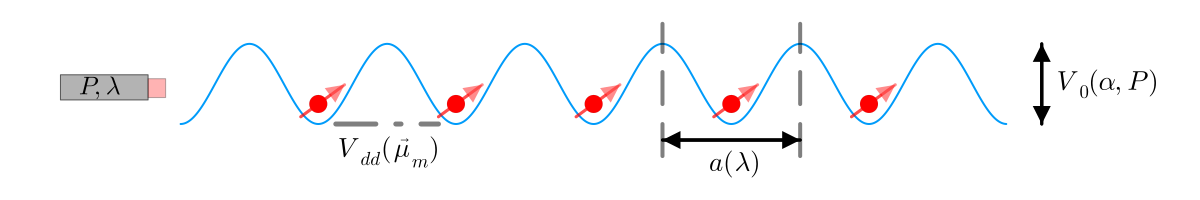
\includegraphics[width=\textwidth]{ch1/mapping.png}
    \end{subfigure}
    \caption{Pictorial representation of ultracold bosons in an optical lattice}
    \label{fig:optical_lattice}
\end{figure}
%%% FIG %%%
\FloatBarrier \!\!\!\!\!\!\!\!\!\!\!

This is, of course, an incredibly simple picture of the setup and there are many more experimentally relevant details that we do not bother with as they do not affect the explorations performed in this thesis. The interested reader may refer to Rudolf et. al. (1999)\cite{grimm1999optical} for a detailed exposition on optical dipole traps for neutral atoms.

\subsection*{Outline of the thesis}

In \autoref{ch1}, we review the basic concepts of a quantum particle trapped in a periodic potential. We introduce the ideas of quasi-momentum, Bloch waves and Wannier functions accompanied with numerical solutions for a particular periodic potential.
\\

In \autoref{ch2}, we proceed to extend our framework to describe the system of interacting bosons in a periodic lattice, thus deriving the Bose-Hubbard model. We also briefly discuss the procedure to map experimental parameters to our theoretical model.
\\

In \autoref{ch3}, we solve the Bose-Hubbard model using various numerical techniques and study the nature of its ground state phases.
\\

In \autoref{ch4}, we analyze a system of bosons with long-range interactions induced by dipole-dipole coupling. This is done by studying the extended Bose-Hubbard model at the mean-field level, thus identifying a variety of new ground state phases that can be realized in the system.
\\

In \autoref{ch5}, we consider spin-1 bosons on a lattice with contact interactions to understand the effect of the spin-degree of freedom on the ground state phases of the Bose-Hubbard model.
\\

In \autoref{ch6}, we analytically study the phenomenon of mediation through bosons by considering a simple impurity model and computing the effective interactions mediated by a conduction band of bosonic atoms on a lattice.
\\

In \autoref{ch7}, we discuss some attempts at extending our analysis beyond the mean-field level. Specifically, we motivate and present the results obtained by utilizing Quantum Monte Carlo techniques to study the finite-temperature physics of the Bose-Hubbard model.
\\

In \autoref{ch8}, we conclude by providing a summary of the results obtained and talk about future prospects for this line of research. 

\setlength{\headheight}{14.5pt}
\pagestyle{fancy}
\fancyhf{}
\renewcommand{\headrulewidth}{1pt}
\renewcommand{\footrulewidth}{0pt}
\renewcommand{\chaptermark}[1]{\markboth{#1}{#1}}
\fancyhead[R]{\thepage}
\fancyhead[L]{\chaptername\ \thechapter\ --\ \leftmark}
\thispagestyle{empty}

\chapter{Quantum mechanics of periodic systems}\label{ch1}

In this chapter, we will review the basic concepts of the physics of a particle trapped in a periodic potential. This will set the stage for extending our formalism to the many-particle system of bosons that we wish to study in this thesis. 

\section{Exploiting structure}
Consider a particle of mass $m$ trapped in a 1D periodic potential $V(x)$ with period $a$. The Hamiltonian can then be written as:
\begin{equation}
    \hat{H} = \frac{\hat{p}^2}{2m} + \hat{V}(x)  \hspace{1cm} V(x + a) = V(x)    
\end{equation}
In an attempt to uncover some structure in this system, let us draw a parallel with the special case of a free-particle where $V(x) = 0$. Such a system has a continuous translation symmetry, i.e, $V(x + a) = V(x) \hspace{0.1cm}\forall a$. As a result of Noether's theorem, the momentum $k$ is a conserved quantity and hence a good quantum number to label the eigenstates. 
\vspace{0.5cm}\\
However, in the case of a periodic potential, the system only has a discrete translation symmetry. Equivalently, the Hamiltonian commutes with the translation operator, $\hat{T}_a = e^{-i\hat{p}a/\hbar}$:
\begin{equation}
    \hat{T}_a \hat{H}\hat{T}_a^{-1} = \hat{H} \hspace{0.5cm}\Longleftrightarrow \hspace{0.5cm}[\hat{T_a}, \hat{H}] = 0
\end{equation}
We can then find the common eigenbasis of $\hat{H}$ and $\hat{T}_a$:
\begin{equation}
    \hat{H}\psi_{E, \alpha}(x) = E\psi_{E, \alpha}(x) \hspace{1cm}\hat{T}_a\psi_{E, \alpha}(x) = \psi_{E, \alpha}(x+a) = e^{i\alpha}\psi_{E, \alpha}
\end{equation}
where the eigenvalues of $\hat{T}_a$ must be pure phases since it is a unitary operator. Now consider the following function $u_{E, \alpha}(x) = e^{-iqx}\psi_{E, \alpha}(x)$ and its behaviour under the action of $\hat{T}_a$:
\begin{align*}
    \hat{T}_a u_{E, \alpha}(x) &= \hat{T}_a e^{-iqx} \psi_{E, \alpha}(x)\\    
    &= e^{-iq(x + a)}\psi_{E, \alpha}(x + a)\\
    &= e^{-iqa}e^{i\alpha}e^{-iqx} \psi_{E,\alpha}(x)\\
    u_{E, \alpha}(x + a) &= e^{i(\alpha - qa)} u_{E, \alpha}(x)
\end{align*}
If we choose to set $\alpha = qa$, $u_{E, \alpha}(x)$ becomes periodic with respect to $x$! Substituting this relation and flipping the definition of $u(x)$ gives us the following result. 
\begin{equation}
    \psi_{E, q}(x) = e^{iqx}u_{E, q}(x) \hspace{1cm}u_{E,q}(x + a) = u_{E, q}(x)
\end{equation}
This is simply a statement of Bloch's theorem, where $\psi_{E, q}$ are the Bloch wave-functions and $q$ is the quasi-momentum. It can be easily seen that $\psi_{E, q}$ is invariant under $q \to q + 2\pi/a$. This is a manifestation of the fact that $q$ belongs to the reciprocal lattice of the system, and it is sufficient to work with the values of $q$ within a single unit cell. Generally, this is chosen to be the Wigner-Seitz cell of the reciprocal lattice, i.e, the first Brillouin zone where $q \in [-\frac{\pi}{a}, \frac{\pi}{a}]$.
\vspace{0.5cm}\\
Applying the time-independant Schr\"{o}dinger equation to the Bloch wave-function, we get:
\begin{equation}
    \hat{H}_q u_q^n(x) = \left [\frac{\hbar^2}{2m}\left (-i\frac{d}{d x} + q \right )^2 + V(x)\right ] u_q^n(x) = E_q^n u_q^n(x)
\end{equation}
where we have replaced $E$ with the band index $n$. This can now be solved to obtain the energy bands and eigenstates of the system. 

\subsection{Bloch wave-functions}
We will proceed to study this system by numerically diagonalizing the Hamiltonian. Let us consider the specific case of $V(x) = V_0 \cos^2(kx)$ such that $V(x + a) = V(x)$ where $a = \pi/k$. In order to simpify the analysis, we begin by introducing some dimensionless variables $\tilde{x} = x/a$ ($\implies \tilde q = \pi q/k$):
\begin{equation}
    \hat{H}_q u_q^n(\tilde x) = \left [\frac{1}{\pi^2}\frac{\hbar^2k^2}{2m}\left (-i\frac{d}{d \tilde x} + \tilde q \right )^2 + V_0\cos^2(\pi\tilde x)\right ] u_q^n(\tilde x) = E_q^n u_q^n(\tilde x)
\end{equation}
As a result of this manipulation, a natural unit of energy has emerged, $E_r = \hbar^2k^2/2m$, which is simply the recoil energy in the context of optical lattices. We can now write the complete dimensionless Hamiltonian as follows: 
\begin{equation}\label{eq:1}
    \hat{H}_q u_q^n(\tilde x) = \left [\frac{1}{\pi^2} \left (-i\frac{d}{d \tilde x} + \tilde q \right )^2 +  \tilde V_0\cos^2(\pi\tilde x)\right ] u_q^n(\tilde x) = \tilde E_q^n u_q^n(\tilde x)
\end{equation}

We will drop the $\sim$ from the variables hereafter but it is implied that we are working with the corresponding dimensionless quantities. It is now sufficient to solve the system within a single unit cell, such that $x \in [-0.5, 0.5]$ and $q \in [-\pi, \pi]$. We now discuss two possible approaches to solve this eigenvalue problem numerically.  

\subsubsection{\large Position basis}
As the equation is already written in the position basis, it seems like a natural choice to use it to construct our Hamiltonian matrix. We start by discretizing our spatial grid $x \in [x_1, x_N]$ into $N$ equally spaced points like so, $x_k = x_1 + (k-1)\Delta x$ where $\Delta x = (x_N - x_1)/N$ and $k \in [1, N]$. 
\vspace{0.5cm}\\
The wavefunction is then represented as a vector of values $u_q^n \equiv [u_q^n(x_1), u_q^n(x_2), \dots, u_q^n(x_N)]$ instead of an analytical expression. Similarly, the potential energy term, $V(x)$, is readily seen as a diagonal matrix with the entries $[V(x_1), V(x_2), \dots, V(x_N)]$. The kinetic energy term, however, requires further consideration. 
$$\left (-i\frac{d}{d x} + q \right )^2 = -\frac{d ^2}{d x^2} - 2iq\frac{d }{d x} + q^2$$
Since our position grid is already discretized, these derivatives can be represented using finite difference schemes like so:

$$\frac{d}{dx}u_q^n(x_k) = \frac{u_q^n(x_{k+1}) - u_q^n(x_{k-1})}{2\Delta x} \hspace{1cm} \frac{d^2}{dx^2}u_q^n(x_k) = \frac{u_q^n(x_{k+1}) - 2u_q^n(x_k) + u_q^n(x_{k-1})}{(\Delta x)^2}$$

This gives us a (nearly) tridiagonal hermitian matrix for the kinetic energy term. 
\vspace{0.5cm}\\
\begin{minipage}{0.6\linewidth}
$$
\hat{H}_k =\frac{1}{\pi^2} \begin{pmatrix}
    \alpha &\beta  &.     &.&.&.&\beta^*\\
\beta^* &\alpha &\beta &.&.&.&.\\
    .      &\beta^*&\alpha&\beta&.&.&.\\
.       &.      &\ddots     &\ddots&\ddots&.&.\\
.       &.      &.     &\beta^*&\alpha&\beta&.\\
.       &.      &.     &.&\beta^*&\alpha&\beta\\
\beta      &.      &.     &.&.&\beta^*&\alpha
\end{pmatrix} 
$$ 
\end{minipage}%
\begin{minipage}{0.3\linewidth}
    \begin{align*}
        \alpha &= 2/(\Delta x)^2 + q^2 \\
        \beta &= -1/(\Delta x)^2- iq/\Delta x
    \end{align*} 
\end{minipage}
\vspace{0.5cm}\\
The elements at the corners of the matrix enforce the periodic boundary condition due to the derivatives coupling the $k = 0$ and $k=N$ position indices. In the absence of these, the matrix would encode a fixed boundary condition, i.e, $u_q^n(x_0) = u_q^n(x_k) = 0$. 
\vspace{0.5cm}\\
At this point, we have completely constructed the Hamiltonian matrix, and its eigenvalues can be obtained using standard diagonalization algorithms. However, it turns out that such a scheme is not very efficient and produces significant deviation of the energy bands near the edges of the first Brillouin zone. This can be understood by interpreting this procedure as expanding the wavefunction using a set of position basis functions, i.e, a set of Dirac deltas, $\delta(x - x_i) \hspace{0.1cm}\forall i \in [1, N]$. As a result, the co-efficient of such basis elements is simply the value of the wavefunction at that position. Such a representation is clearly a poor choice for the system since we have not leveraged its periodicity in any way.

\subsubsection{\large Fourier basis}
In order to choose a better basis, we note that $V(x)$ and $u_q^n(x)$ have the same periodicity. We can then expand them as a discrete Fourier sum using a plane-wave basis.
\begin{equation}\label{eq:2}
    V(x) = \sum_m V_m e^{2\pi imx} \hspace{1cm} u_q^n(x) = \sum_m c_m^{n,q} e^{2 \pi i mx}
\end{equation}
Note that we are still working with the dimensionless variables. Substituting Eq. \eqref{eq:2} in Eq. \eqref{eq:1}, we get an expression for the kinetic energy, which is diagonal in this basis:
\begin{equation}\label{eq:ke}
    \frac{1}{\pi^2} \left (-i\frac{d}{dx} + q\right )^2u_q^n(x) = \sum_m \left (2m + \frac{q}{\pi} \right )^2 e^{2\pi imx} c_m^{n,q}
\end{equation}
Similarly, the potential energy is given by:
\begin{equation}\label{eq:pe}
    V(x)u_q^n(x) = \sum_m \sum_{l'} V_m e^{2\pi i(m + l')x}c_{l'}^{n,q} = \sum_m \sum_l V_m e^{2\pi ilx} c_{m-l}^{n,q}
\end{equation}
It is also readily seen that our specific choice of the lattice potential only results in three non-zero coefficients of the Fourier sum.
\begin{equation}\label{eq:pef}
    V(x) = V_0 \cos^2(\pi x) = \frac{V_0}{4}(e^{2\pi ix} + e^{-2\pi ix} + 2)
\end{equation}
Putting together Eq. \eqref{eq:ke}, Eq. \eqref{eq:pe} and Eq. \eqref{eq:pef}, we can write the Schr\"{o}dinger equation as a matrix equation:
\begin{equation}
    \sum_{m'} H_{m, m'} \cdot c_{m'}^{n,q} =\epsilon_q^n c_m^{n,q}
\end{equation}
where the matrix form of the Hamiltonian is determined as follows:
\begin{equation}
    H_{m,m'}  = \begin{cases} 
        \left (2m + \frac{q}{\pi} \right )^2 + V_0/2 & \text{if } |m - m'| = 0 \\
        V_0/4 & \text{if } |m - m'| = 1 \\
        0 & \text{otherwise} 
     \end{cases}
\end{equation}
Since this basis set implicitly takes the periodicity of the system into account, we do not have to restrict our analysis within a particular unit cell. At this point, the Fourier expansion runs over infinite terms, so we will have to truncate it at an arbitrary $m_{max}$ such that $m \in [-m_{max}, m_{max}]$ resulting in a matrix of dimension $(2m_{max} + 1) \cross (2m_{max} + 1)$. It turns out that a very small value of $m_{max}$ $(\sim 10)$ is sufficient to study the lowest energy bands. In comparison, we required $N \sim 100$ when we used the position basis.
\newpage
\subsection{Results}
%%% FIG %%%
\begin{figure}[!htb]
    \centering
    \begin{subfigure}[b]{\textwidth}  %keep total sum <1 to show in same line
        \centering
        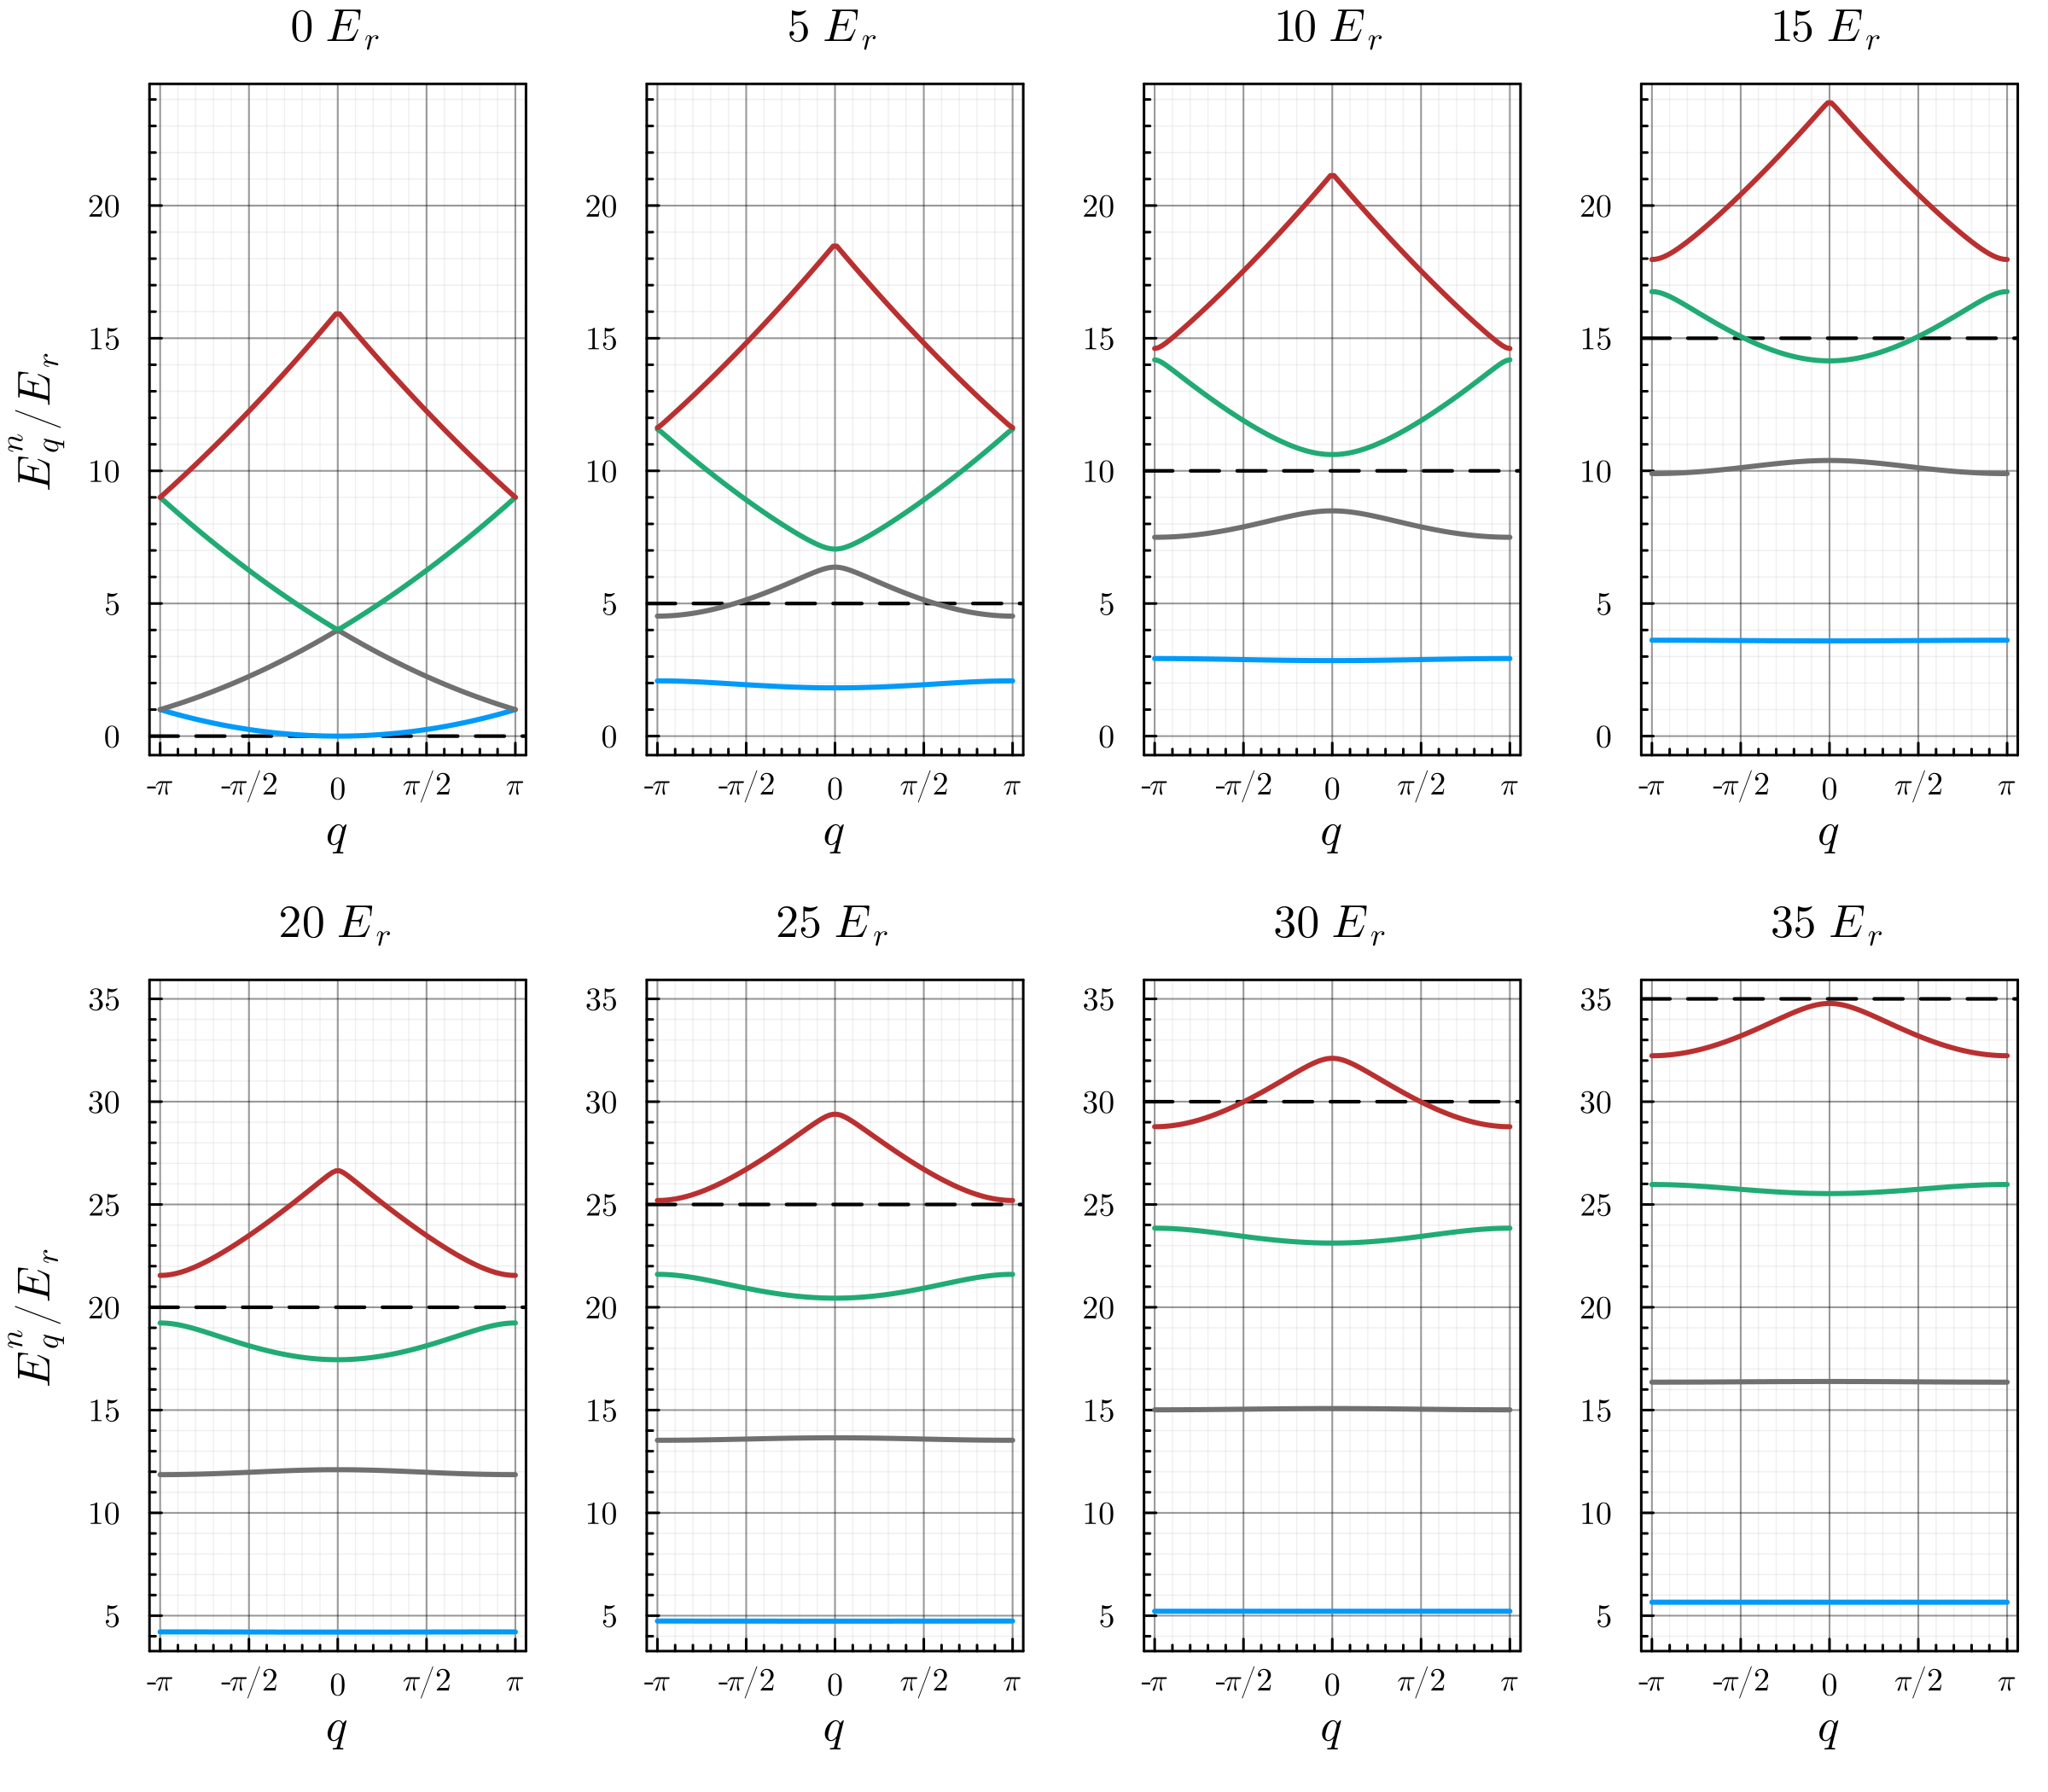
\includegraphics[width=\textwidth]{ch2/energy_bands.png}
    \end{subfigure}
    \caption{First four energy bands of a 1D lattice for various lattice potentials. The black dashed line indicates the lattice depth.}
    \label{fig:bands}
\end{figure}
%%% FIG %%%
\FloatBarrier \!\!\!\!\!\!\!\!\!\!\!

In Fig. \ref{fig:bands} we have plotted the energy bands for the 1D system by diagonalizing the Hamiltonian in the Fourier basis. We see that for the free particle case $(V=0)$, we have the usual parabolic band structure. However, as the lattice potential is increased, band gaps emerge and the widths of the lower bands become smaller, resulting in equally spaced flat bands. This is expected since we can approximate the minima of the periodic potential as a harmonic oscillator for large $V$. 
%%% FIG %%%
\begin{figure}[!htb]
    \centering
    \begin{subfigure}[b]{\textwidth}  %keep total sum <1 to show in same line
        \centering
        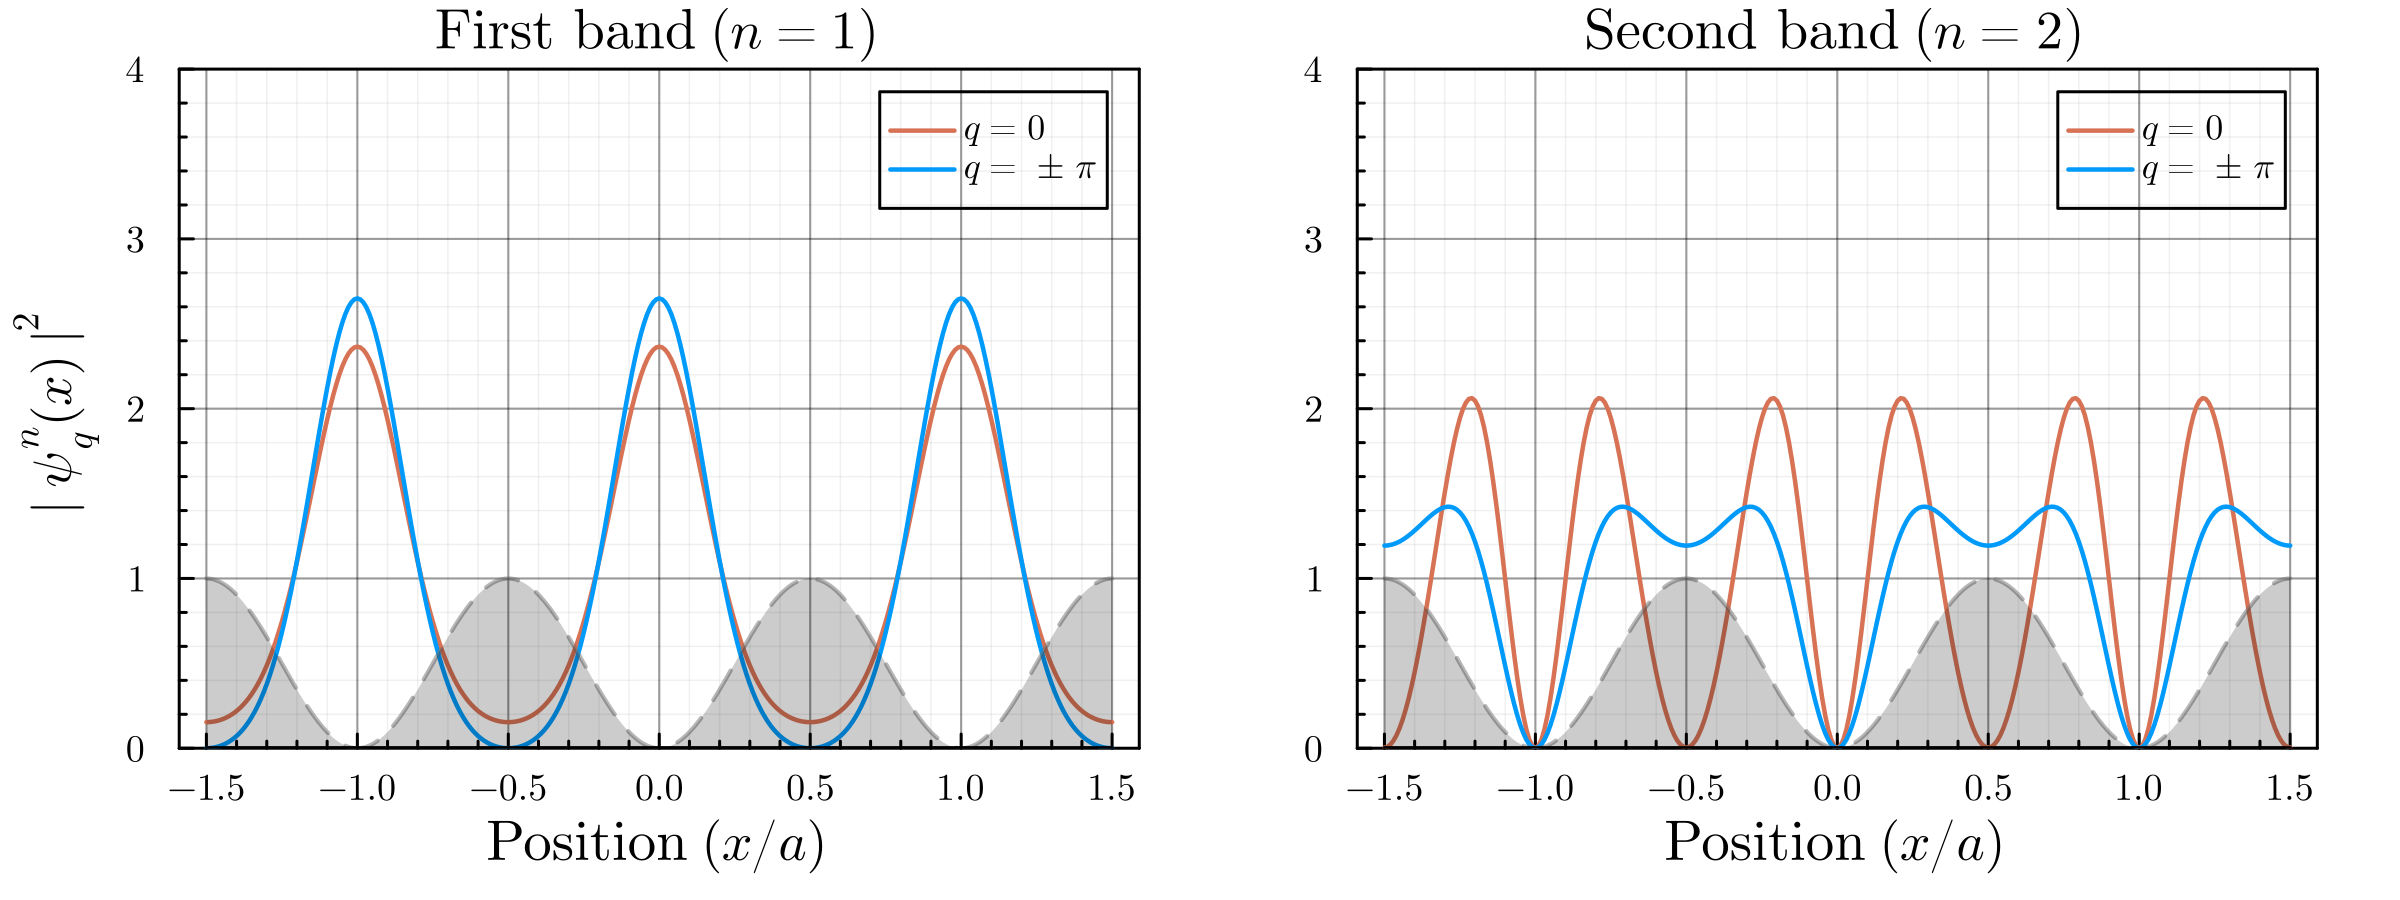
\includegraphics[width=\textwidth]{ch2/bloch_wf.png}
    \end{subfigure}
    \caption{Probability distribution of Bloch wave-functions for $V_0 = 5E_r$. The lattice potential (black) is plotted to indicate the periodicity of the system.}
    \label{fig:bloch}    
\end{figure}
%%% FIG %%%
\FloatBarrier \!\!\!\!\!\!\!\!\!\!\!

\section{Constructing a localized basis}
While the Bloch wavefunctions form a perfectly valid basis set for a periodic system, they are also delocalized across the entire lattice as seen in Fig. \ref{fig:bloch}. Such a situation is rather cumbersome to work with, as will become clear in the next chapter when we discuss the formalism to describe many-particle physics. Instead, we look for a localized basis set.  
\vspace{0.5cm}\\
A simple recipe can be obtained by drawing a parallel with the free-particle case once again. We know that the energy eigenstates are plane waves which are delocalized across all space, and performing a Fourier transformation from $k \to x$ gives us Dirac delta functions, which are highly localized. Similarly, the quasi-momentum $q$ plays the role of $k$ here and by performing a Fourier transform over the first Brillouin zone, we can construct a new basis by introducing a conjugate variable $R$ that is analogous to $x$. 
\begin{equation}
    \phi^n_R(x) = \frac{1}{N}\sum_{q \in BZ} e^{-iqR} \psi_q^n(x)
\end{equation}
where $\psi_q^n(x)$ are the Bloch wave-functions of the $n$th band, $N$ is the number of unit cells in the lattice and $\phi_R^n(x)$ are the so-called \textit{Wannier} functions. An immediate consequence of this procedure is that the Wannier functions are no longer energy eigenstates, but that is a fair price to pay for a localized basis. Also note that $R$ can take the values $na$ where $a$ is the lattice spacing, and $n \in \mathbb{Z}$.
%%% FIG %%%
\begin{figure}[!htb]
    \centering
    \begin{subfigure}[b]{\textwidth}  %keep total sum <1 to show in same line
        \centering
        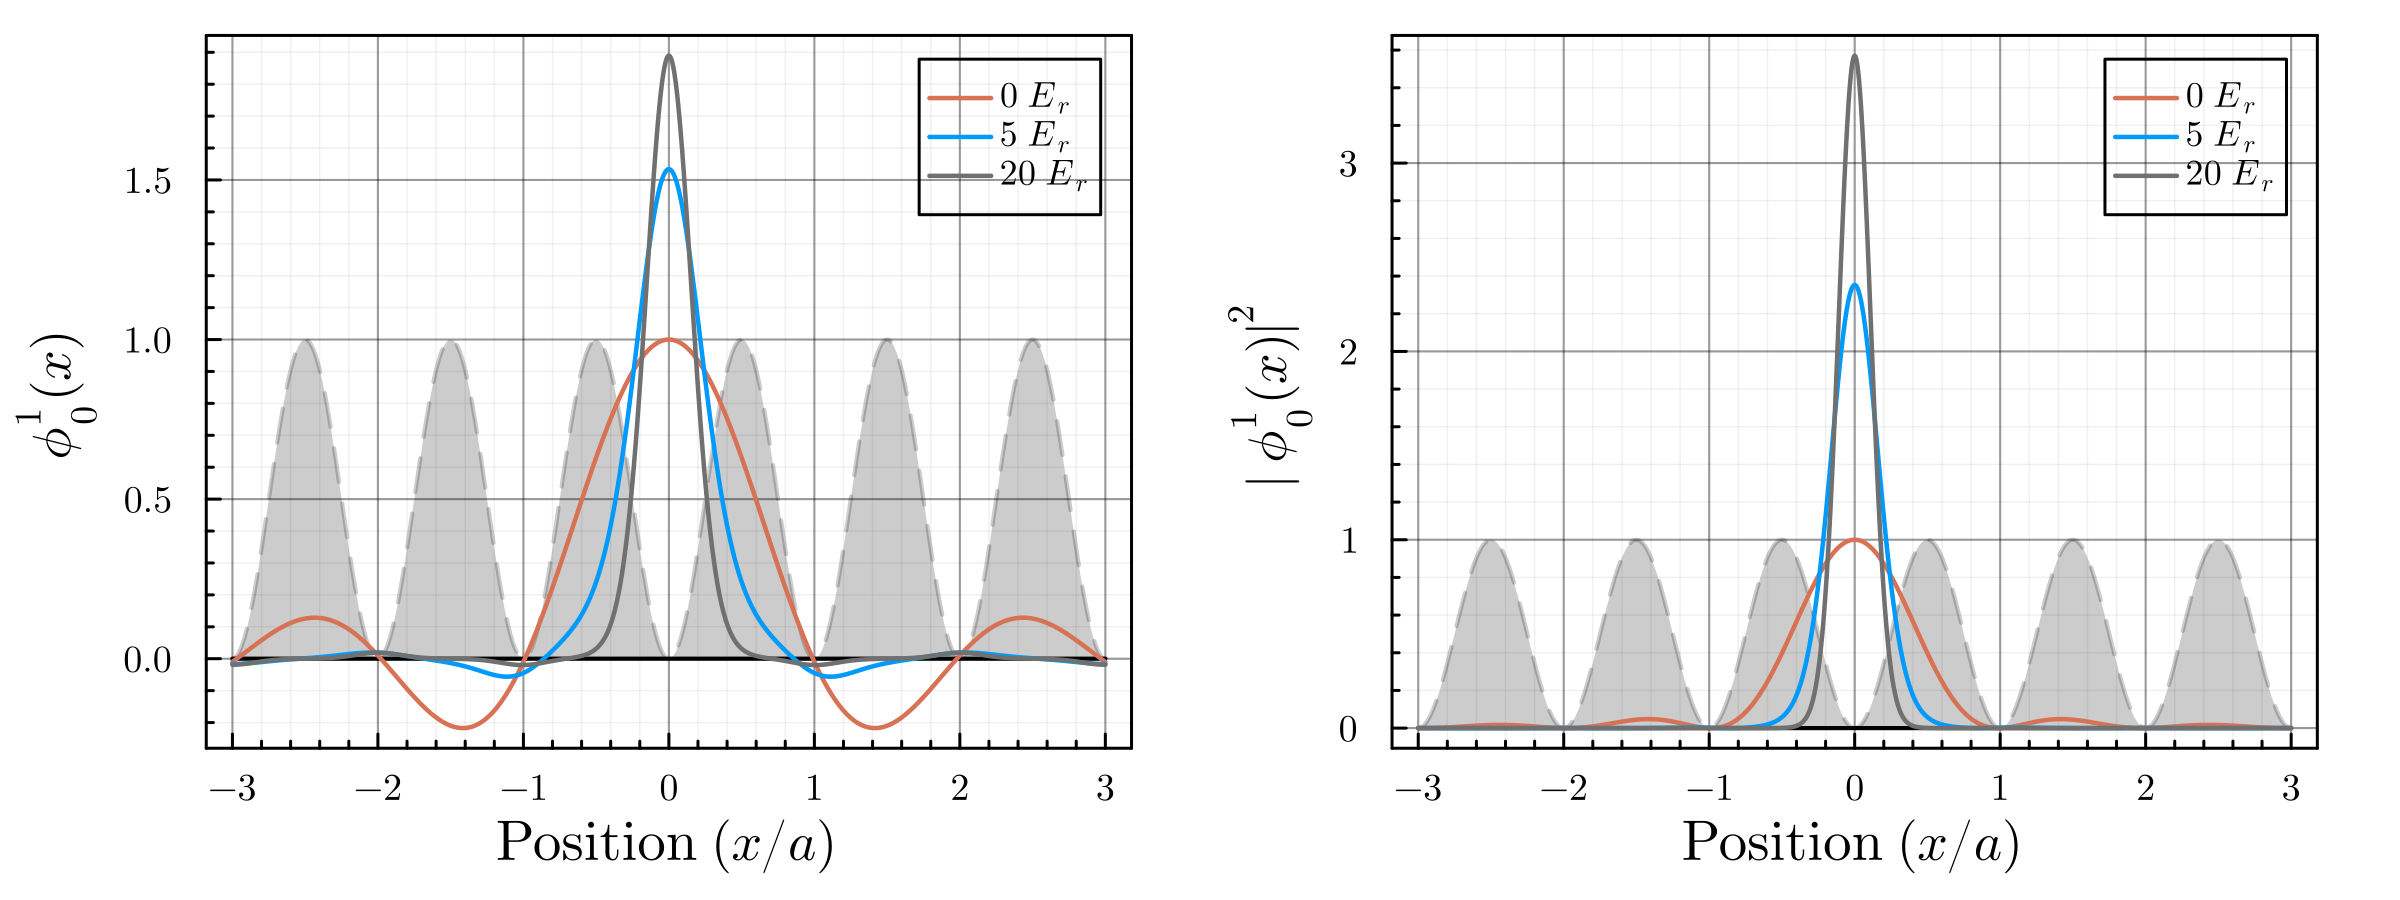
\includegraphics[width=\textwidth]{ch2/wannier_wf.png}
    \end{subfigure}
    \caption{Probability amplitude and density of Wannier wave-functions for Wannier functions of the lowest band. The lattice potential (black) is plotted to indicate the periodicity of the system.}
    \label{fig:wannier}
\end{figure}
%%% FIG %%%
\FloatBarrier \!\!\!\!\!\!\!\!\!\!\!

We see from Fig. \ref{fig:wannier} that as the lattice depth is increased, the Wannier function becomes more localized. In fact, as mentioned earlier, a deep lattice potential can be approximated as a harmonic well and the corresponding Wannier function approaches a gaussian. Let us now try to ascribe meaning to the conjugate index $R$, by considering the following expression for some $m \in \mathbb{Z}$.
\begin{align*}
    \phi_{R+ma}^n(x) &= \frac{1}{N}\sum_{q \in BZ} e^{-iqR} e^{-iqma} \psi_q^n(x)\\    
    &= \frac{1}{N}\sum_{q \in BZ} e^{-iqR} \psi_q^n(x - ma)\\
    &= \phi_{R}^n(x - ma)
\end{align*}
We see that translation in $R$ corresponds to simply shifting the Wannier function in real space by the same amount! This motivates the fact that $R$ is simply an index to label the lattice site on which the Wannier function is localized. 

\subsection{Gauge freedom and non-uniqueness}
At this point, we must bring up a peculiar feature of the Bloch wavefunctions, namely that there exists a gauge freedom in its definition.
\begin{equation}
    \tilde \psi_q^n(x) \equiv e^{i\chi_n(q)} \psi_q^n(x)
\end{equation}
where $\chi_n(q)$ can be any arbitrary function over the reciprocal lattice vectors and cannot be determined from the Schr\"{o}dinger equation. More generally we can describe it in terms of a unitary operation, $U$, like so:
\begin{align}
    \tilde \psi_q^n(x) &= \sum_{m =1}^N U_{mn}^{(q)} \psi_q^n(x)\\
    \phi^n_R(x) &= \frac{1}{N}\sum_{q \in BZ} e^{-iqR} \tilde\psi_q^n(x)
\end{align}
This gauge freedom clearly carries over to the Wannier functions, rendering them non-unique! Luckily, this does not change the fact that any choice of Wannier functions will still be localized, just that they may have different 'shapes'. This motivates the existence of a possibly unique set of Wannier functions that are \textit{maximally localized}\cite{Pavarini2011TheLA}. For instance, such a set may be determined by minimizing the variance of the position operator.
\begin{equation}
    \Omega = \sum_n \langle x^2 \rangle_n  - \langle x \rangle^2_n
\end{equation}
Things can get even more complicated when the energy bands are close enough to intersect, in which case we must allow mixing of the Wannier functions with respect to the $n$ index as well\cite{Marzari_2012, Walters_2013}. However, for the purpose of this thesis, we do not take these complexities into account and simply proceed with the choice of $\chi_n(q) = 0$. This suffices for a rough order of magnitude calculation to motivate the discussions in the following chapters.

\chapter{The Bose-Hubbard model}\label{ch2}
Now that we have set up the basic framework to describe the physics of a single particle trapped in a periodical potential, we will proceed to use it to develop a description of a system of interacting bosons in an optical lattice.

\section{Derivation}\label{sec:bhmderiv}
Consider a system of spinless bosons of mass $m$ trapped in an optical lattice potential, $V_{\text{lat}}(r)$ with $M$ sites. The physics of the system is described by the following second-quantized Hamiltonian\cite{Fetter}.
\begin{equation}\label{eq:tise_second}
    H = \int d^3r \cdot \Psi(r) \left [ -\frac{\hbar^2}{2m}\nabla^2 + V_{\text{lat}}(r) \right ] \Psi(r) + \frac{1}{2}\int d^3r \int d^3r' \Psi^{\dagger}(r)\Psi^{\dagger}(r')U_{int}(r, r')\Psi(r)\Psi(r')
\end{equation}
where $U_{int}(r,r')$ describes the interaction between the bosons, and $\Psi(r)$, $\Psi^{\dagger}(r)$ are the bosonic field operators, fulfilling the bosonic commutation relations:
\begin{equation}
    [\Psi(r), \Psi^{\dagger}(r')] = \delta(r -r') \hspace{1cm} [\Psi(r), \Psi(r')] = 0 \hspace{1cm} [\Psi^{\dagger}(r), \Psi^{\dagger}(r')] = 0
\end{equation}
Our first approximation can be motivated by observing the energy band gaps in Fig. \ref{fig:bands}. As long as the interaction energies of the trapped bosons are much smaller than the first energy gap, we can assume that the physics are mostly dominated by the lowest energy band. We can then expand the field operators in terms of a basis of Wannier functions of the first band.
\begin{equation}
    \Psi(r) = \sum_j \phi_j(r) \cdot a_j    
\end{equation}
where $a_j$ ($a_j^{\dagger}$) creates (annihilates) a particle localized at the $j$-th lattice site in the lowest band. The bosonic operators $a_j$, $a_j^{\dagger}$ satisfy the following commutation relations:
\begin{equation}\label{eq:ccr}
    [a_j, a_l^{\dagger}] = \delta_{j, l} \hspace{1cm} [a_j, a_l] = 0 \hspace{1cm} [a_j^{\dagger}, a_l^{\dagger}] = 0
\end{equation}
Upon making this substitution, we arrive at the following Hamiltonian:
\begin{equation}
    H = -\sum_{i, j} t_{i, j} a_i^{\dagger}a_j + \frac{1}{2}\sum_{i, j, k, l} U_{i, j, k, l} a_i^{\dagger} a_j^{\dagger}a_l a_k
\end{equation}
where $t_{i, j}$ and $V_{i, j, k, l}$ are defined as follows:
\begin{equation}\label{eq:hopping_param}
    t_{i, j} = \int d^3r \cdot \phi_i(r) \left [ -\frac{\hbar^2}{2m}\nabla^2 + V_{\text{lat}}(r)\right ] \phi_j(r)
\end{equation}

\begin{equation}\label{eq:interact_param}
    U_{i, j, k, l} = \frac{1}{2}\int d^3r\int d^3r' \cdot \phi_i(r)\phi_j(r') U_{int}(r, r')\phi_k(r)\phi_l(r')    
\end{equation}
For sufficiently deep optical lattices, only the nearest neighbour tunnelling amplitudes are significant ($t_{i, i+1} \gg t_{i, i+2}$) precisely because the Wannier functions are highly localized. This motivates the tight-binding approximation where we neglect all the coupling terms beyond the nearest neighbors. Note that we use $\langle i, j\rangle$ to indicate a sum over nearest neighbour indices including $(i, j)$ and $(j, i)$.
\begin{equation}
    H = -\sum_{\langle i, j \rangle}t_{i, j} a_i^{\dagger}a_j + \frac{1}{2}\sum_{i, j, k, l} U_{i, j, k, l} a_i^{\dagger} a_j^{\dagger}a_l a_k
\end{equation}
At this point, based on the type of interaction between the bosons, we can obtain various flavours of the model\cite{Dutta_2015}. For now, we will consider the simplest case of contact interaction, which is a pseudo-potential that we can introduce to model the low energy scattering physics\cite{reichl}.
\begin{equation}
    U_{int}(r,r') = \frac{4\pi\hbar^2 a_s}{m} \delta(r - r') = g\delta(r - r')
\end{equation}
where $a_s$ is the s-wave scattering length of the bosons. As a result of the short range nature of this interaction, there is only one non-zero matrix element from the interaction term, namely, that of on-site repulsion, $U = U_{iiii}$. Upon considering an isotropic lattice ($t_{i j} \equiv t$, $U_{iiii} \equiv U$), we obtain the central theme of this thesis, the Bose-Hubbard Hamiltonian.
\begin{equation}\label{eq:bhm}
    H = -t\sum_{\langle i, j \rangle} a_i^{\dagger}a_j + \frac{U}{2}\sum_{i} n_i(n_i - 1)    
\end{equation}
\section{Ground state phases}
To begin understanding the physics of this system, we note that it has two competing terms. The interplay between them gives rise to two distinct quantum phases that can be classified by analyzing the limiting cases of the Hamiltonian. For simplicity, we will work in the grand-canonical ensemble with the Hamiltonian, $H_{GCE} = H-\mu\sum_i n_i$.

\subsection{Mott Insulator}
Let us consider the limit $t \ll U$ of Eq. \eqref{eq:bhm}.
\begin{equation}\label{eq:tlim}
    H = \frac{U}{2}\sum_i n_i(n_i - 1) - \mu \sum_i n_i
\end{equation}
Such a Hamiltonian only contains the pairwise on-site interaction energy of bosons occupying the same lattice site. We can think of $n_i(n_i - 1)/2$ as arising from ${}^n C_ 2$ which counts the pairs of bosons on each site. This term tends to minimize the fluctuation of the occupation number by localizing the bosons onto the lattice sites.
\vspace{0.5cm}\\
Since Eq. \eqref{eq:tlim} is simply a sum over single-site Hamiltonians which are all equivalent, the ground state solution is a pure Fock state. 
\begin{equation}
    \ket{\Psi} = \bigotimes_{i = 1}^{M} \ket{n} = \underbrace{\ket{n, n, \dots, n}}_{\text{M sites}}
\end{equation}
with ground state energy $E_{gs} = \sum_i E_i$ such that:
\begin{equation}
    E_i = \frac{U}{2}n(n - 1) - \mu n \hspace{1cm} n = \left \lfloor{\frac{\mu}{U}}\right \rfloor  + 1
\end{equation}
Thus, the Mott insulator phase is described by a state with integer occupation on each lattice site. Further, it is a gapped phase  as it requires finite energy to generate excitations (i.e. remove a boson from one site and add it to another), and it is characterized by zero compressibility ($\partial N/\partial \mu = 0$)\cite{Bloch_2008}.

\subsection{Superfluid}
Let us now consider the other limit, $t \gg U$ of Eq. \eqref{eq:bhm}. 
\begin{equation}
    H = -t\sum_{\langle i, j \rangle} a_i^{\dagger}a_j - \mu \sum_i n_i
\end{equation}
This is simply a non-interacting tight-binding model in the second quantized notation. The 'hopping' term $a_i^{\dagger}a_j$ annihilates a particle at the $j$th site and creates a particle at the $i$th site. Such a Hamiltonian tends to maximize the fluctuations of the occupation number by delocalizing the bosons across the entire lattice.
\vspace{0.5cm}\\
It is trivially diagonalizable by switching to the Bloch basis ($\{\tilde{a}_k\}$):
\begin{equation}
    a_i = \frac{1}{\sqrt{M}}\sum_k e^{-ikr_i} \tilde{a}_k
\end{equation}
\begin{equation}
    H = \sum_k (\epsilon_k - \mu) \tilde{a}_k^{\dagger}\tilde{a}_k
\end{equation}
where $\epsilon_k$ is the dispersion relation determined based on the lattice geometry. The ground state is then simply a condensate in the $k=0$ state:
\begin{equation}
    \ket{\Psi} = (\tilde{a}_0^{\dagger})^N \ket{0} = \left (\frac{1}{\sqrt{M}}\sum_{i = 1}^M a_i \right )^N \ket{0}
\end{equation}
Although it is not strictly true\cite{schmets2008teaching}, we will consider a non-ideal Bose-Einstein condensate to be equivalent to a superfluid in this thesis. Such a phase is gapless and only requires arbitrarily small energy to generate excitations\cite{Bloch_2008}.

\subsection{Quantum phase transition}
From the above discussion, we see that the Mott insulator and Superfluid phases are quite distinct in their properties. Although this characterization was performed in the extreme limits, we expect that in the complete Hamiltonian, Eq. \eqref{eq:bhm}, the true phases would broadly have the same properties. The true ground states, however, may be different due to the presence of particle-hole excitations.
\vspace{0.5cm}\\
As a result, even at $T=0$, we expect a transition to occur between the Mott insulator and Superfluid phases. Such a transition is facilitated by quantum fluctuations rather than thermal ones. In the next chapter, we will try to generate the corresponding phase diagram using various numerical techniques.

\section{Connecting theory and experiment}\label{sec:calc_params}
Before we proceed further, it is prudent to note that the Bose-Hubbard parameters, $t$ and $U$ are not independant as is apparent from the derivation in Sec. \ref{sec:bhmderiv}. We will explore this fact by explicitly computing these parameters for a 1D lattice. 
\vspace{0.5cm}\\
Let us begin with the hopping parameter as defined in Eq. \eqref{eq:hopping_param} and perform some manipulations to recast it into a surprisingly succinct form.
\begin{align}
    t_{ij} &= -\int d^3r \ \phi_i^* \left [ -\frac{\hbar^2}{2m}\nabla^2 + V_{\text{lat}}(r) \right ] \phi_j \nonumber\\ 
    &= -\int d^3r \left (\frac{1}{\sqrt{N}} \sum_{q} e^{iq\cdot r_i} \psi_q^* \right ) \left [ -\frac{\hbar^2}{2m}\nabla^2 + V_{\text{lat}}(r) \right ] \left (\frac{1}{\sqrt{N}} \sum_{q'} e^{iq'\cdot r_i} \psi_{q'}\right ) \nonumber\\ 
    &= -\frac{1}{N}\sum_{q q'} e^{iq \cdot r_i} \cdot e^{iq' \cdot r_j} \int d^3r \ \psi_q^* \left [ -\frac{\hbar^2}{2m}\nabla^2 + V_{\text{lat}}(r)\right ] \psi_{q'} \nonumber\\
    &=  -\frac{1}{N}\sum_{q q'} e^{iq \cdot r_i} \cdot e^{iq' \cdot r_j} \cdot \delta_{q q'} \epsilon_{q} \nonumber \\
    t_{ij}&= -\frac{1}{N}\sum_{q} \epsilon_{q} \cdot e^{i q \cdot (r_i - r_j)}
\end{align}
where $\epsilon_q$ is the disperson relation. This tells us that the tunneling amplitude is simply a Fourier transform of the energy dispersion of the system. On the other hand, the on-site interaction parameter is computed quite directly from Eq. \eqref{eq:interact_param} as follows.
\begin{equation}
    U = g\int d^3r |w(r)|^4    
\end{equation}

%%% FIG %%%
\begin{figure}[!htb]
    \centering
    \begin{subfigure}[b]{\textwidth}  %keep total sum <1 to show in same line
        \centering
        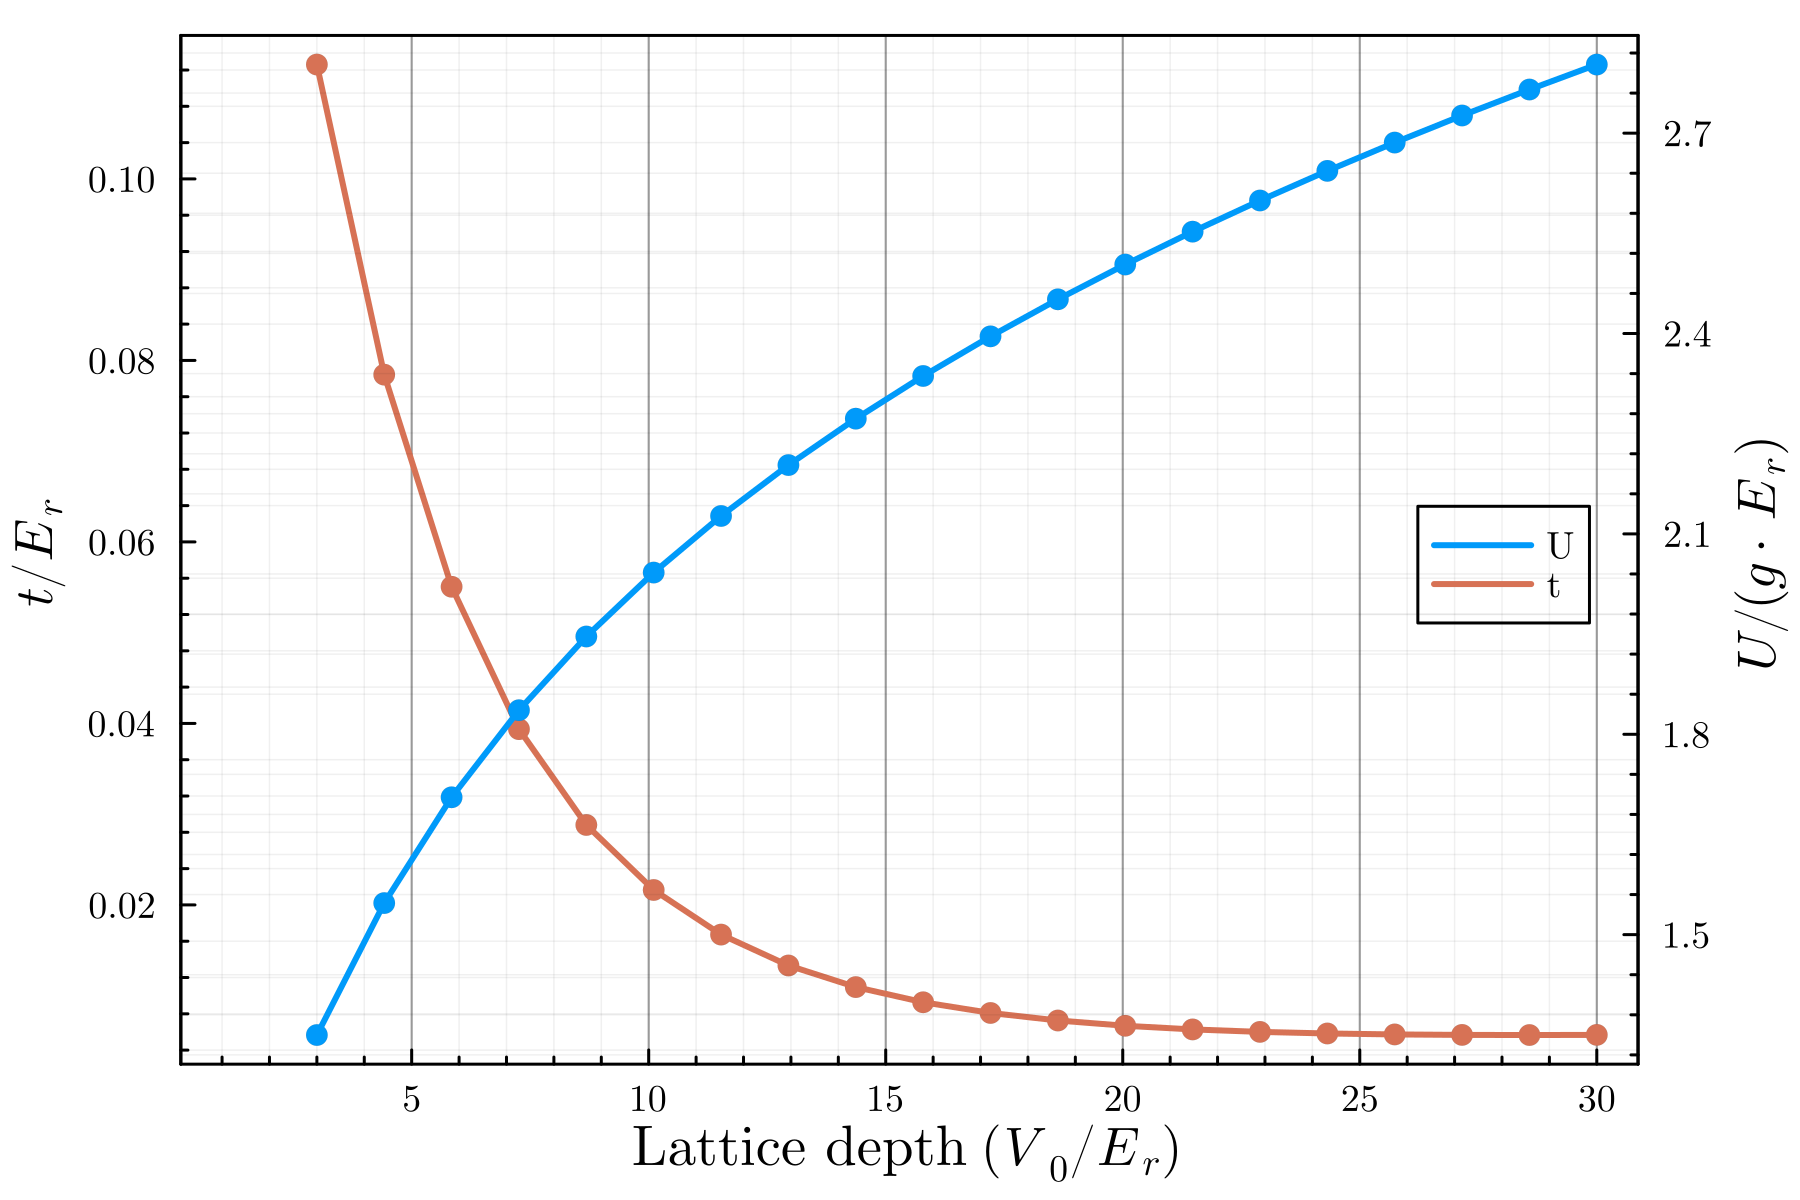
\includegraphics[width=0.75\textwidth]{ch3/bhm_parameters.png}
    \end{subfigure}
    \caption{Bose-Hubbard parameters in a 1D system for various lattice depths.}
    \label{fig:bhm_param}
\end{figure}
%%% FIG %%%
\FloatBarrier \!\!\!\!\!\!\!\!\!\!\!

We see that the parameters are dependant in Fig. \ref{fig:bhm_param}. At this point, it seems that once we have fixed the lattice potential (and hence, the Wannier functions upto a gauge), the parameters $t$ and $U$ are uniquely determined. This would severely restrict the regimes of the Bose-Hubbard model that are experimentally accessible. However, we have not taken into the account the co-efficient $g$ in the interaction parameter. Particularly, the s-wave scattering length $a_s$ can be tuned using Feshbach resonances\cite{Chin_2010}, thus restoring our ability to explore the parameter space. 
\vspace{0.5cm}\\
For the rest of this thesis, we will study the phase diagram of the Bose-Hubbard model as if $t$ and $U$ are independant, in order to gain a complete understanding of the various phases hosted by it. However, experimentally traversing these diagrams would require the construction of paths by taking their dependance into account.


\chapter{Solving the Bose-Hubbard model}\label{ch3}
Consider the 1D Bose-Hubbard Hamiltonian, with $N$ bosons and $M$ lattice sites:
\begin{equation}\label{eq:bhm1}
    H = -t\sum_{\langle i, j\rangle} a_i^{\dagger}a_j + \frac{U}{2}\sum_i n_i(n_i - 1) - \mu \sum_i n_i
\end{equation}
In this chapter, we will review some numerical techniques to study the phases exhibited in this model. Although the 1D model is exactly solvable using a Bethe ansatz\cite{Fabio11}, these techniques are easily extended to higher dimensions and other lattice geometries where an exact solution might not exist.

\section{Exact Diagonalization}
We begin with the most naive approach of exactly diagonalizing the Hamiltonian. A natural basis to construct the many-body Hamiltonian is the set of Fock states, $\{\ket{n_1, n_2, \dots, n_M}\}$ defined as the simultaneous eigenstates of the site-wise number operators.
\begin{equation}
    \hat{n}_i \ket{n_1, n_2, \dots, n_M} = n_i \ket{n_1, n_2, \dots, n_M}
\end{equation}
such that $\sum_{i = 1}^{M} n_i = N$ and $n_i \geq 0$. 
\vspace{0.5cm}\\
Constructing this basis is equivalent to the combinatorics problem of enumerating all the ways of distributing $N$ objects in $M$ boxes. It follows that the dimensionality of the Hilbert space is given by $d = (M+N-1)!/N!(M-1)!$. We can now compute the matrix elements of the Hamiltonian, $\bra{u}H\ket{v}$, using the following relations that follow from the bosonic commutation relations in Eq. \eqref{eq:ccr}.
\begin{align}
&\hat{a}_i \ket{n_1, n_2, \dots, n_i, \dots, n_M} = \sqrt{n_i} \ket{n_1, n_2,  \dots, n_i - 1, \dots, n_M}\\
&\hat{a}_i^{\dagger} \ket{n_1, n_2, \dots, n_i, \dots, n_M} = \sqrt{n_i + 1} \ket{n_1, n_2,  \dots, n_i + 1, \dots, n_M}
\end{align}
Due to the large dimension of such a matrix, a complete diagonalization would be computationally expensive and wasteful since we only aim to study the ground state properties. As a result, an iterative procedure such as the Lanczos algorithm \cite{Pavarini2011TheLA} would be a better choice since it only computes the extreme eigenvalues and eigenvectors of large matrices. We now proceed to discuss some observables that can be used to track the phase transition.

\subsection{Observables}
Consider the single particle density matrix, $n^{(1)}(r, r') = \langle \Psi(r)^{\dagger} \Psi(r') \rangle$ where $\Psi(r), \Psi(r')$ are the bosonic field operators introduced in Eq. \eqref{eq:tise_second}. This is a matrix with respect to ($r$, $r'$) and can be used to formulate a rigorous definition of a BEC by writing it in its diagonal form.
\begin{align}
    n^{(1)}(r, r') &= \sum_i n_i \cdot \psi_i^*(r)\psi_i(r') \nonumber \\
    &= n_0 \cdot \psi_0(r)^*\psi_0(r') + \sum_{i\neq 0}  n_i \cdot \psi_i^*(r)\psi_i(r')
\end{align}
where $n_i$ and $\{\psi_i(r)\}$ are the eigenvalues and single-particle eigenstates of $n^{(1)}(r, r')$, respectively. These states $\{\psi_i(r)\}$ are not necessarily eigenstates of the single-particle Hamiltonian.
\\
\\
Note that we have separated the term with the largest eigenvalue $(n_0)$ from the sum. We can now define a condensate fraction, $f = n_0/N$, which will be macroscopic $(f \sim 1)$ when the system is in a BEC phase and vanishes otherwise. As a result, when we consider the limit $|r - r'| \to \infty$ in the BEC phase, while most of the sum will interfere destructively and cancel out, the first term may have a non-zero contribution\cite{leggett2008}.
\begin{equation}\label{eq:odlro}
    \lim_{|r-r'|\to \infty}  n^{(1)}(r, r') \neq 0
\end{equation}
This condition is known as Off-Diagonal Long-Range Order (ODLRO), and will be useful in deriving the order parameter in the mean-field analysis.

\subsection{Results}
%%% FIG %%%
\begin{figure}[!htb]
    \centering
    \begin{subfigure}[b]{0.45\textwidth}  %keep total sum <1 to show in same line
        \centering
        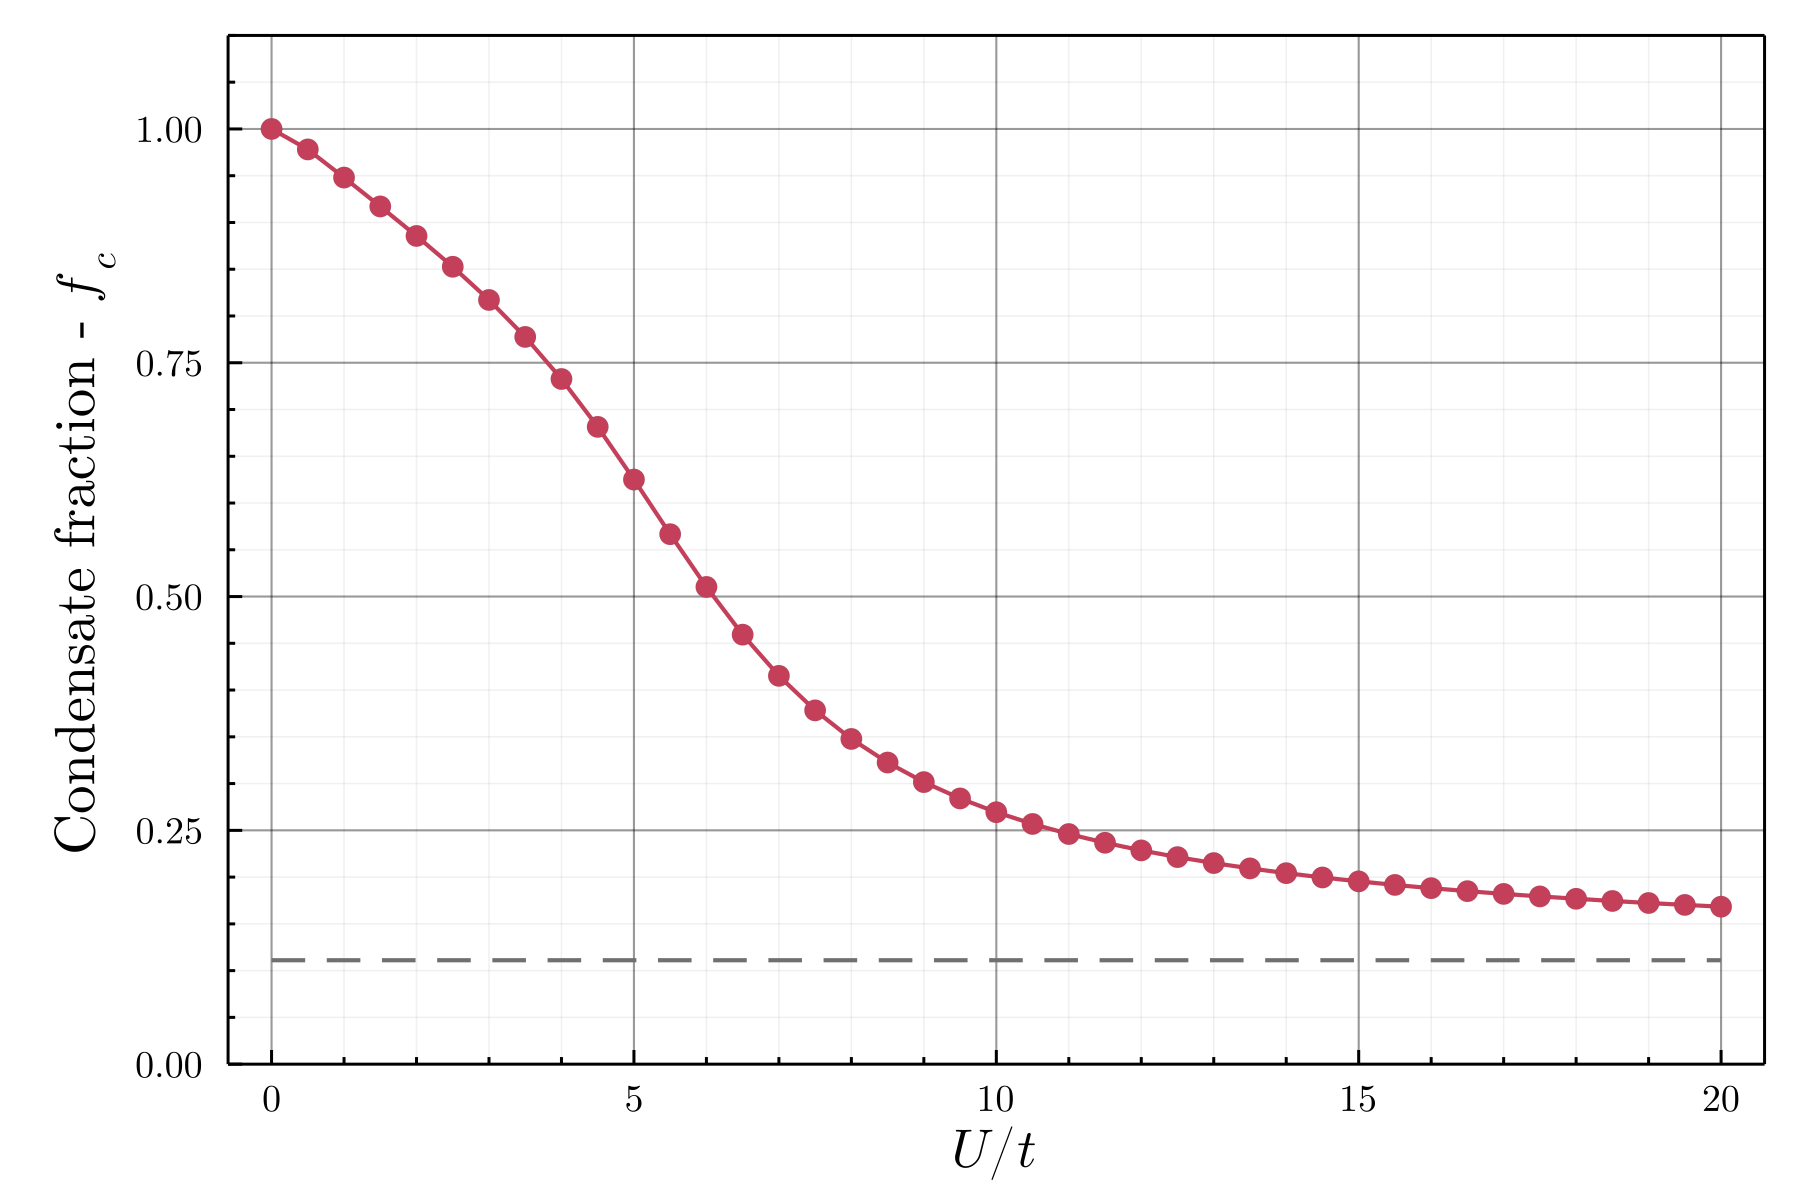
\includegraphics[width=\textwidth]{ch4/condensate_fraction.png}
        \caption{Condensate fraction}
        \label{fig:cond_frac}
    \end{subfigure}
    \hspace{1em}  %\hfill
    \begin{subfigure}[b]{0.45\textwidth}
        \centering
        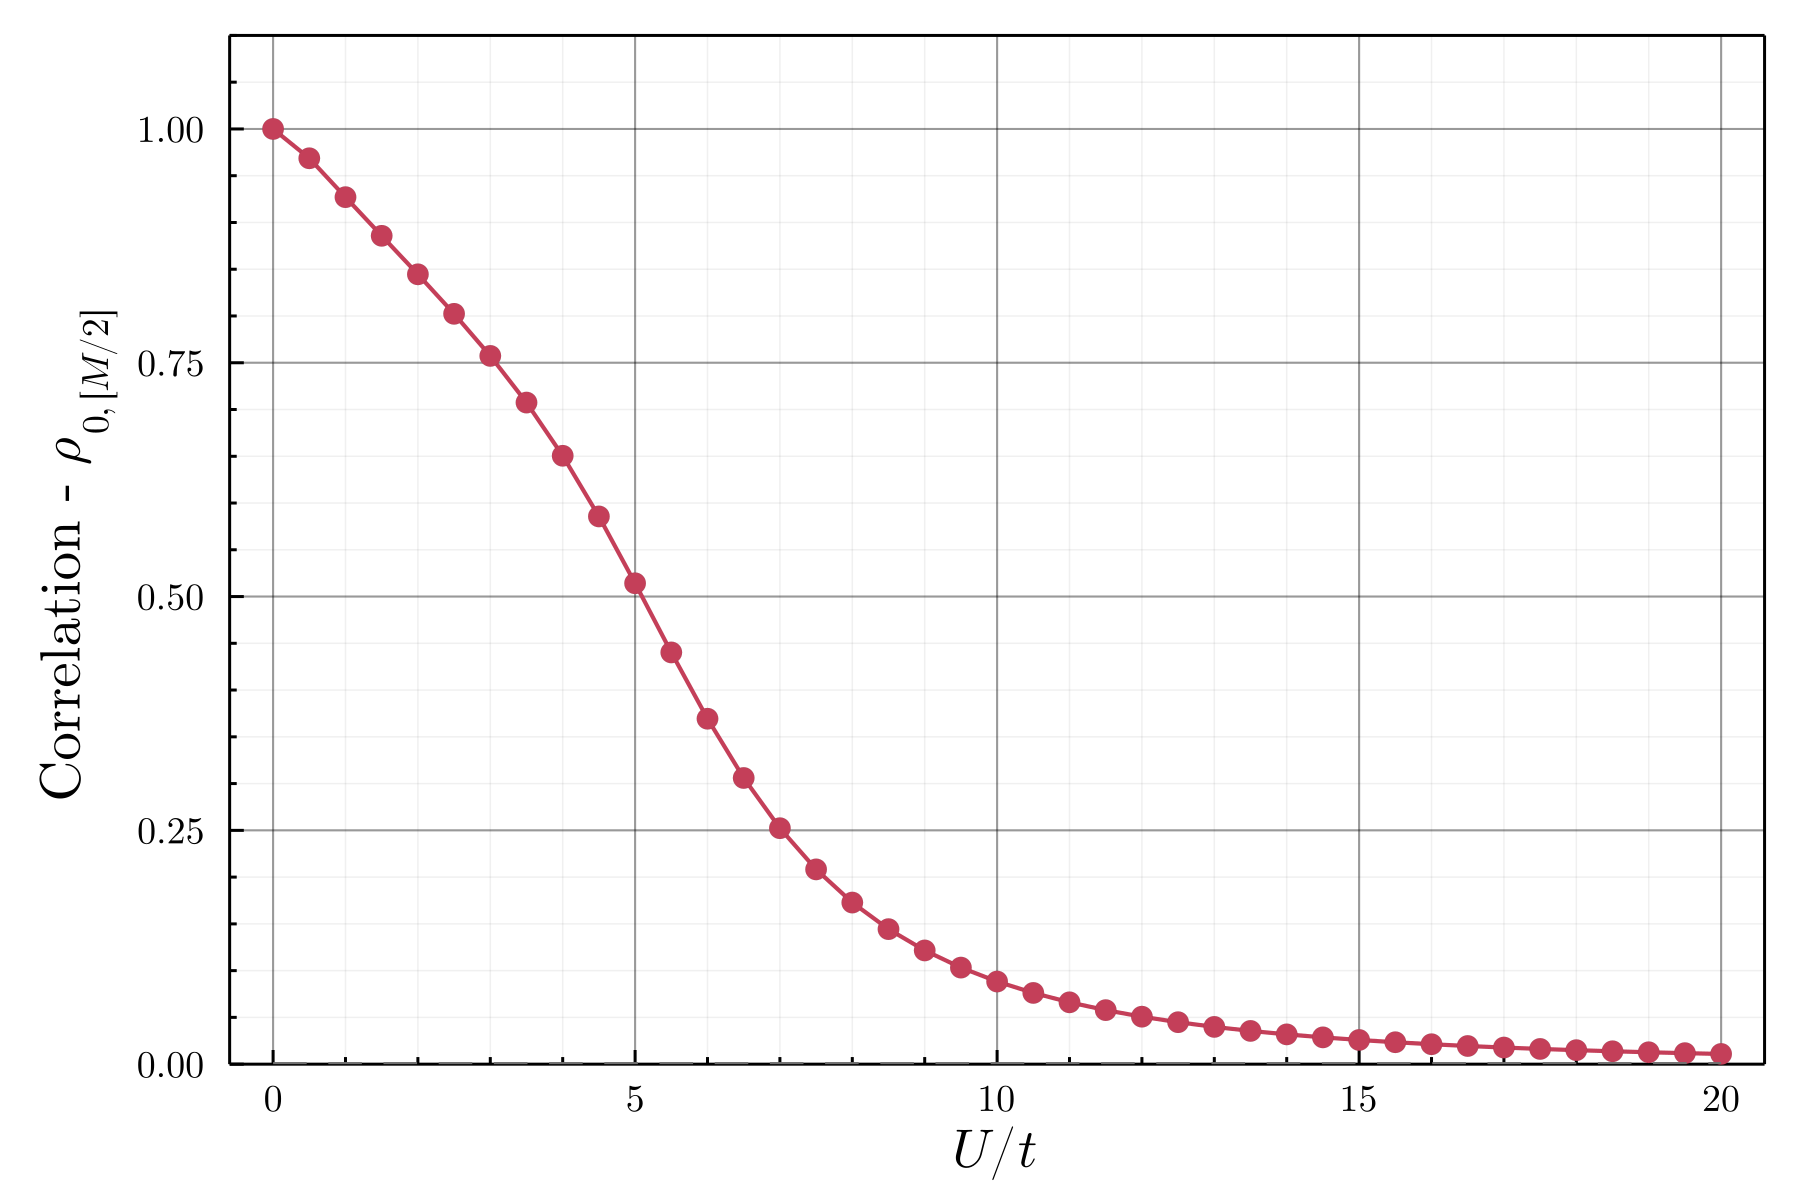
\includegraphics[width=\textwidth]{ch4/odlro.png}
        \caption{Off-diagonal Long-range order}
        \label{fig:odlro}
    \end{subfigure}
    \caption{Tracking the phase transition using various observables ($N = M = 9$)}
    \label{fig:ed_track}
\end{figure}
%%% FIG %%%
\FloatBarrier \!\!\!\!\!\!\!\!\!\!\!

We see in Fig. \ref{fig:cond_frac} that the condensate fraction, $f$, quickly drops from $1$ as $U/t$ is increased. However, note that it never vanishes even for arbitrarily small $U/t$, against our expectations for the Mott insulator phase. This turns out to be an artifact of the finite size of the system. Since the eigenvalues of the SPDM must satisfy $n_0 \geq 1$, we have $f \geq 1/M$ which would vanish for large $M$. 
\vspace{0.5cm}\\
On the other hand, in Fig. \ref{fig:odlro} we have plotted the matrix element of the SPDM with the farthest indices, in an attempt to capture the ODLRO condition. Surprisingly, we do see that the element starts off at $1$ and quickly vanishes in the Mott insulator regime, even though the condition of $|i-j| \to \infty$ cannot really be achieved in such a small system.
\vspace{0.5cm}\\
There is also another observable that is worth tracking, namely, the average variance of the number operator on an arbitrary lattice site, $\langle \delta n^2\rangle$. Since the Mott insulator phase is expected to be a pure Fock state, the occupation variance must vanish. 

%%% FIG %%%
\begin{figure}[!htb]
    \centering
    \begin{subfigure}[b]{0.52\textwidth}  %keep total sum <1 to show in same line
        \centering
        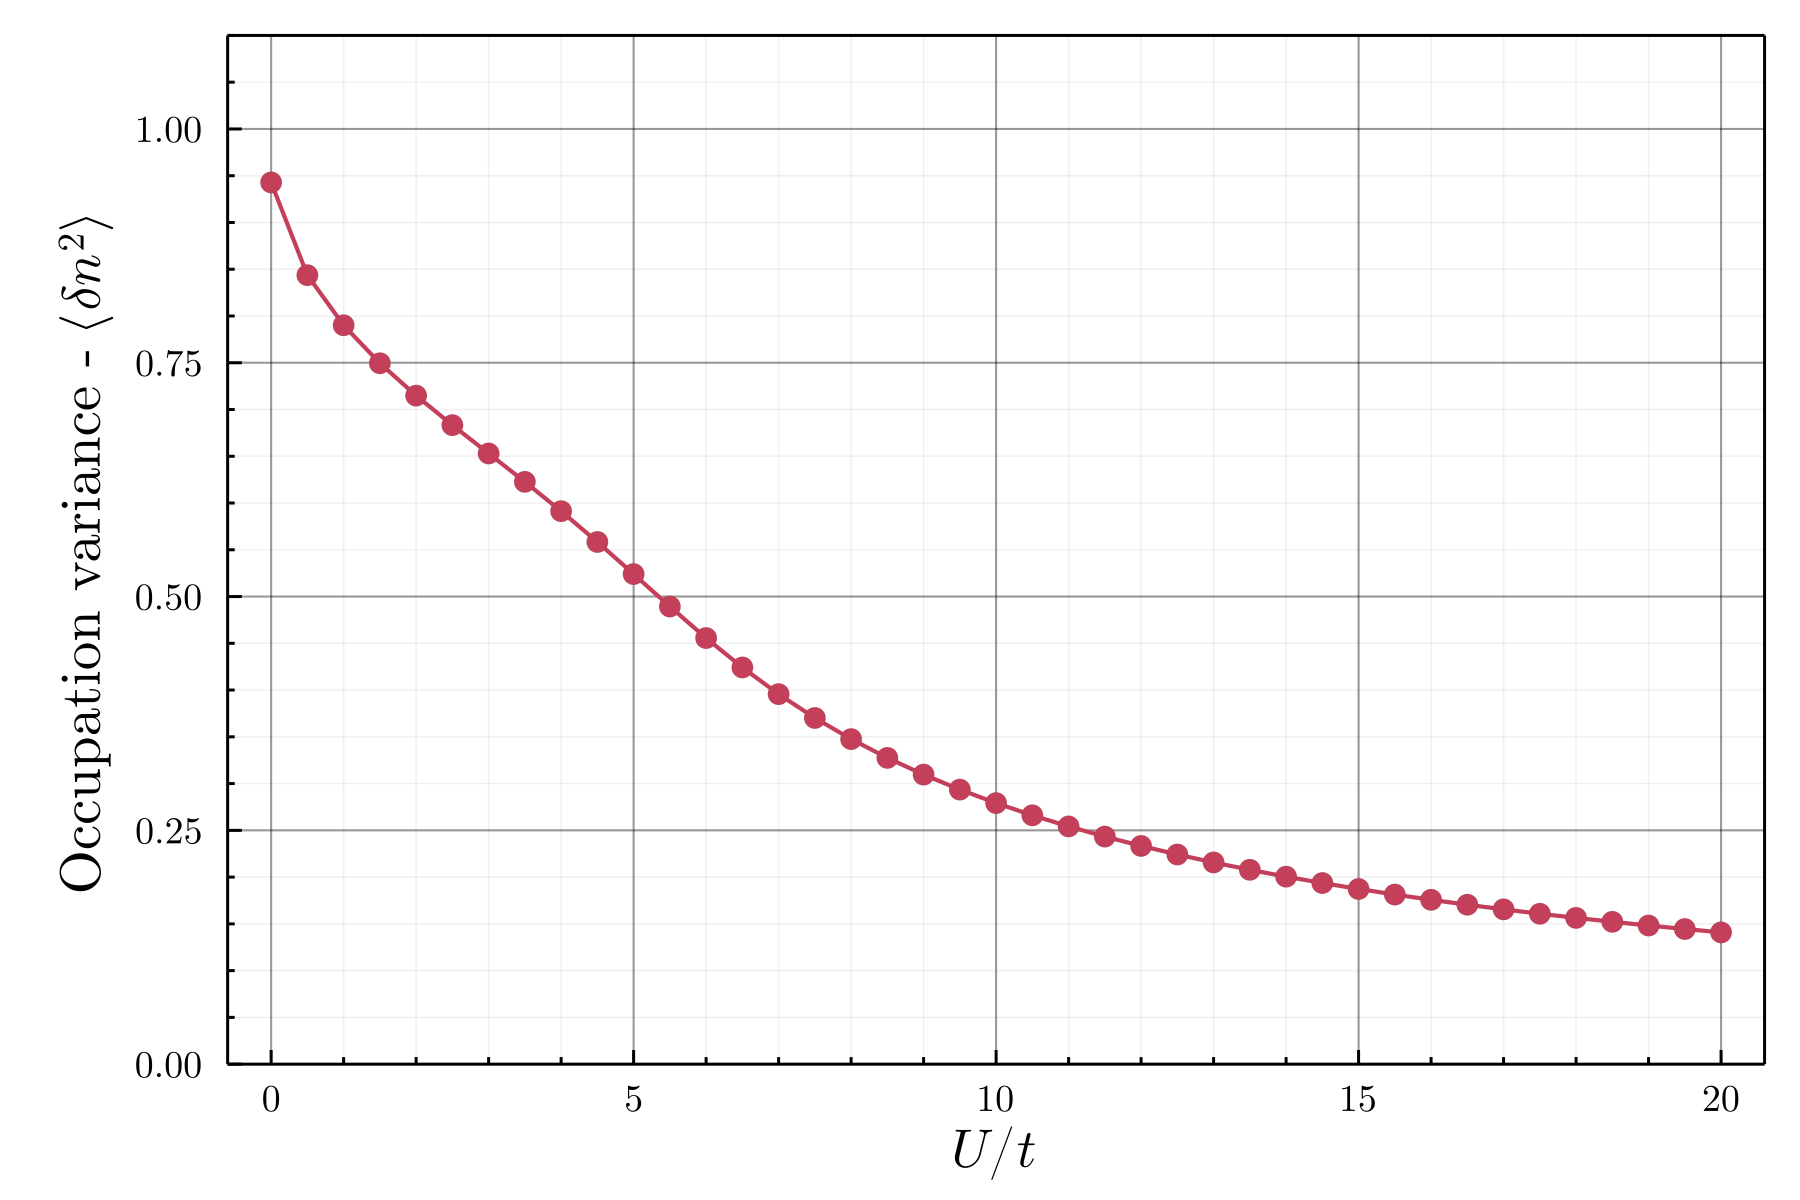
\includegraphics[width=\textwidth]{ch4/occupation_var.png}
        \caption{Canonical ensemble $(N=9, M=9)$}
        \label{fig:occ_var}
    \end{subfigure}
    \hspace{1em}  %\hfill
    \begin{subfigure}[b]{0.38\textwidth}
        \centering
        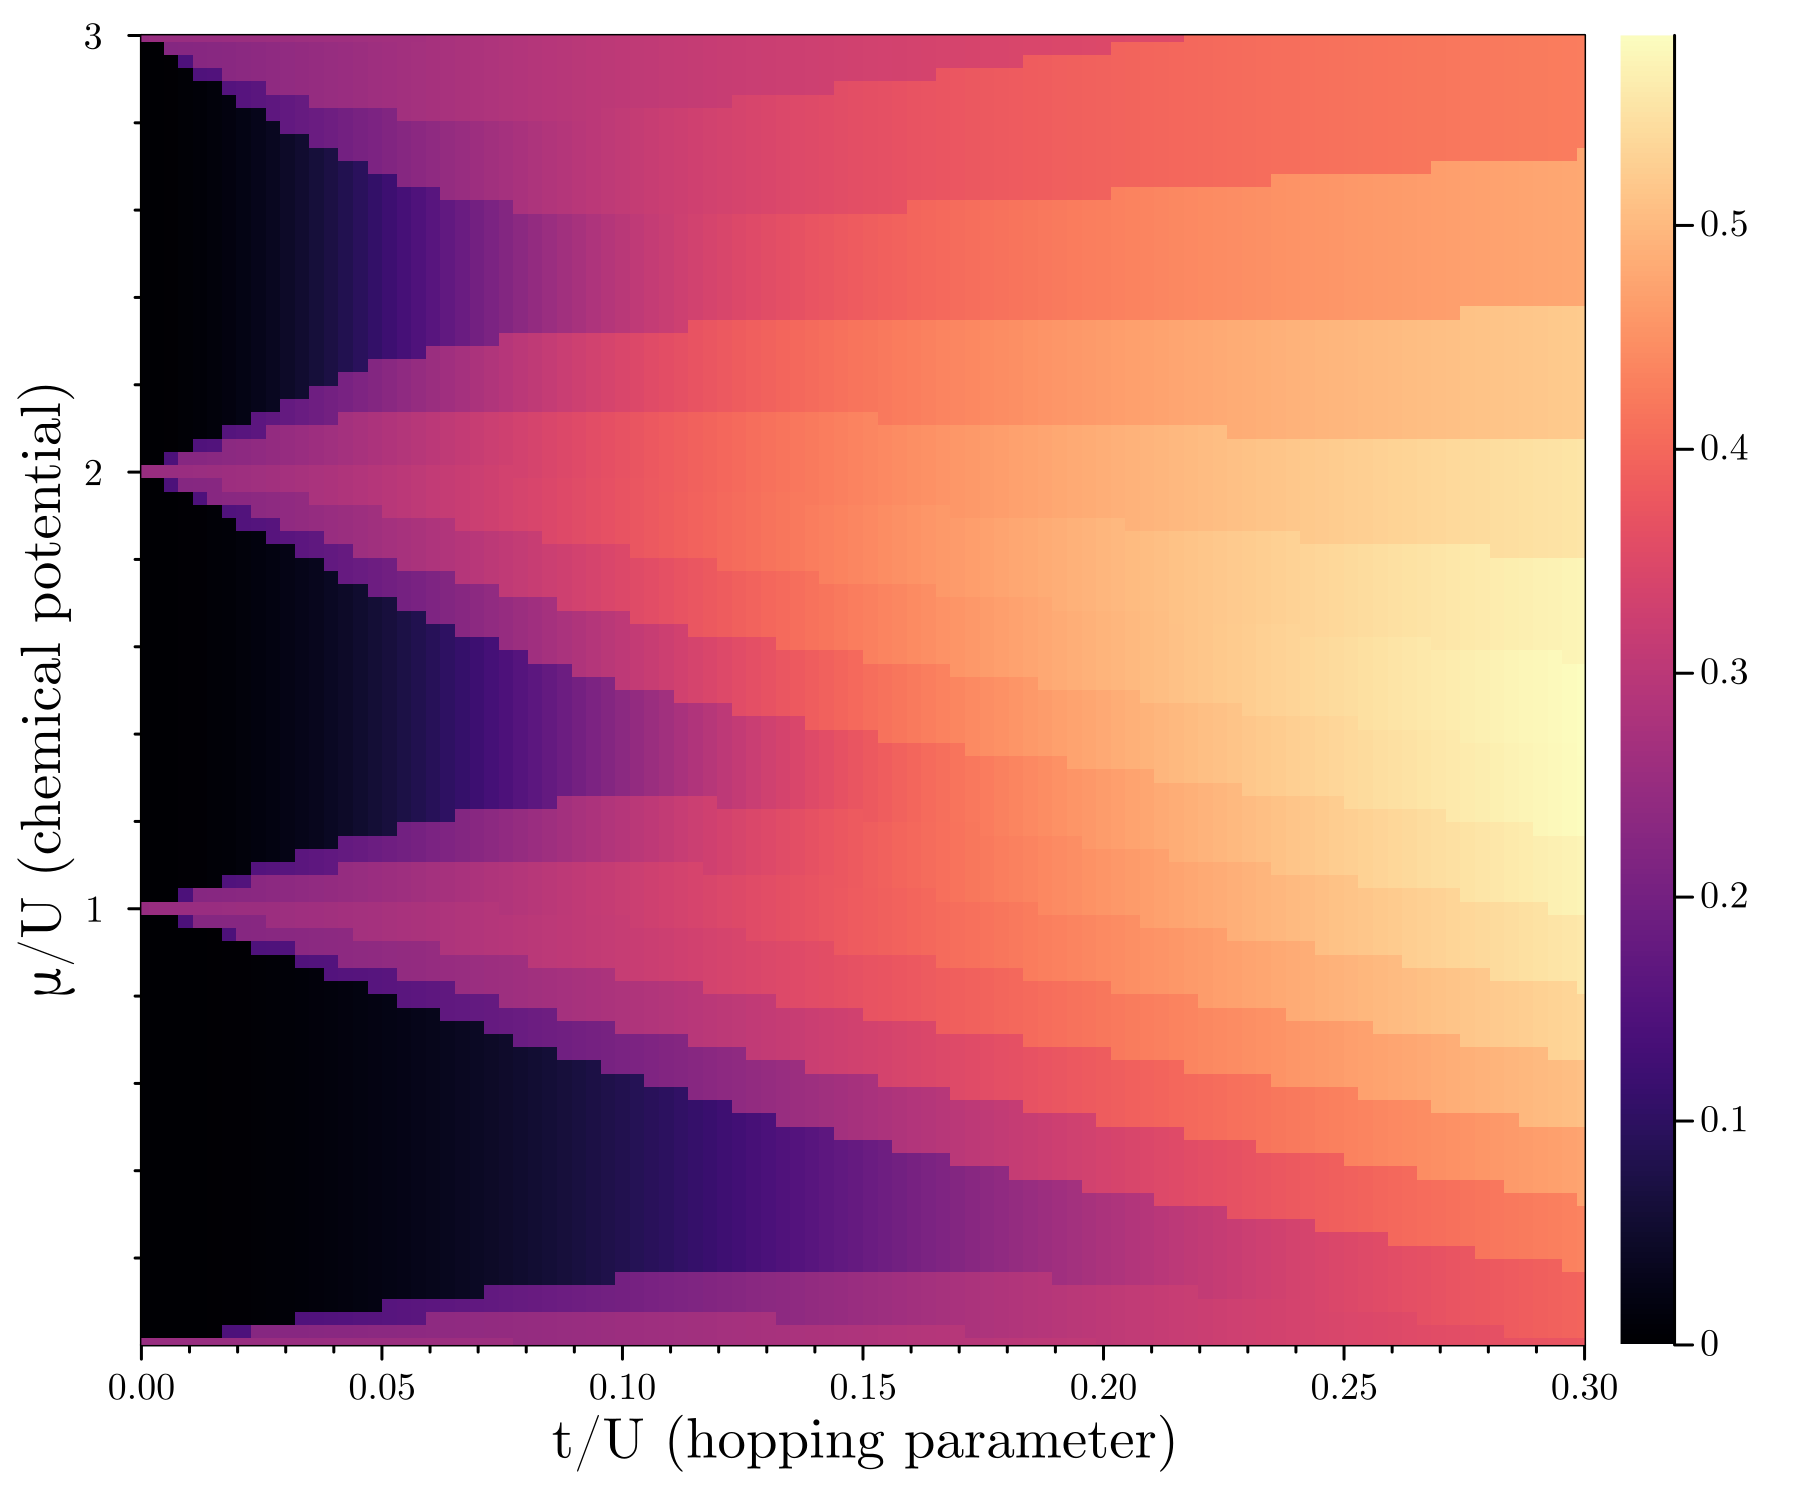
\includegraphics[width=\textwidth]{ch4/phase_diagram_ed.png}
        \caption{ Grand canonical ensemble $(N_{max} = 4, M = 6)$}
        \label{fig:phasediagram_ed}
    \end{subfigure}
    \caption{Tracking the phase transition using average variance of occupation number}
    \label{}
\end{figure}
%%% FIG %%%
\FloatBarrier \!\!\!\!\!\!\!\!\!\!\!

Unsurprisingly, Fig. \ref{fig:occ_var}, also demonstrates a curve with a similar trend as the ones in Fig. \ref{fig:ed_track}. Although there seems to be some signatures of the quantum phase transition, it seems that the Mott insulator phase strictly only exists for $U/t \to \infty$  ($\implies t/U = 0$). However, note that these results were obtained from an exact diagonalization over a fixed-$N$ subspace of the Fock space. If we allow variable particle number (upto an arbitrary cut-off, $N \in [0, N_{max}]$) by considering a grand canonical ensemble instead, we can gain some more insight. We see that this is indeed the case, as the phase diagram obtained in Fig. \ref{fig:phasediagram_ed} suggests that the Mott insulator phase could exist in an extended region away from $t/U = 0$.
\vspace{0.5cm}\\
However, it is dubious to make this claim rigorously since all of our possible order parameters are muddled by the finite (and small!) lattice size that we have considered. One could extend this analysis by exactly diagonalizing a larger system, however, the computational cost increases exponentially and quickly becomes unfeasible after $\sim 20$ sites. Instead, we will proceed to explore some approximate methods that allow us to get more qualitative but well-defined results. 

\section{Mean Field Theory}\label{sec:bhm_mft}
The motivation for this technique is the fact that diagonalizing the BHM in either of the extreme limits is trivial, however the dimensionality of the Hilbert space blows up in the general case, Eq. \eqref{eq:bhm1}. Note that we will continue working exclusively in the grand canonical ensemble. 
%%% FIG %%%
\begin{figure}[!htb]
    \centering
    \begin{subfigure}[b]{\textwidth}  %keep total sum <1 to show in same line
        \centering
        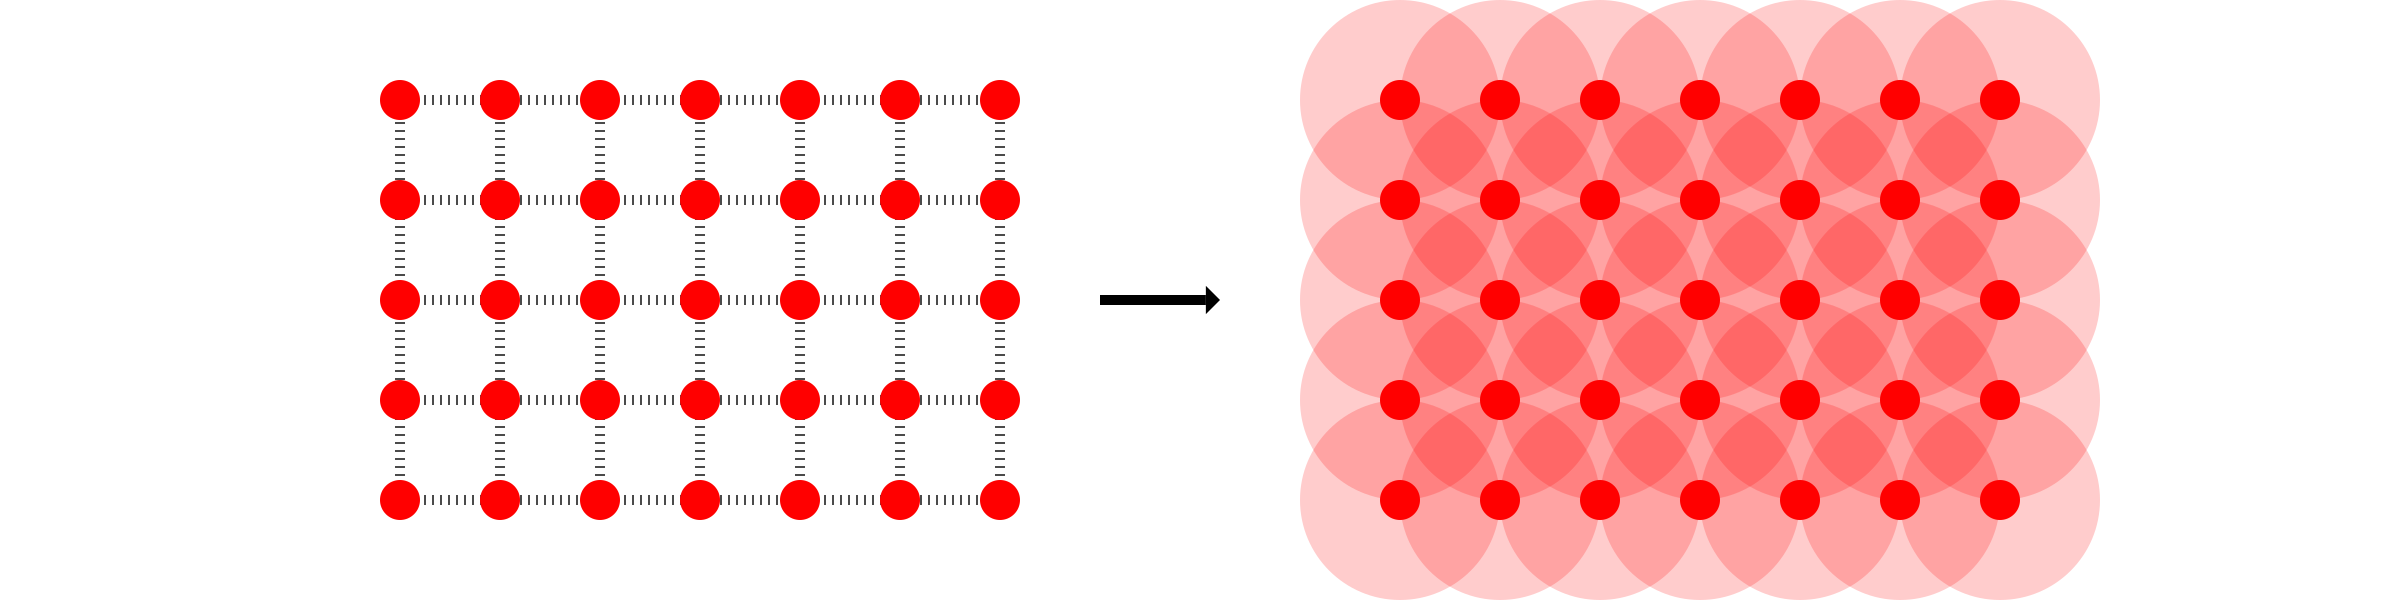
\includegraphics[width=\textwidth]{ch4/MFTdiagram.png}
    \end{subfigure}
    \caption{Pictorial representation of MFT in 2D}
    \label{}
\end{figure}
%%% FIG %%%
\FloatBarrier \!\!\!\!\!\!\!\!\!\!\!

In order to extract some qualitative features of the model, we attempt a de-coupling which results in a system with a smaller Hilbert space. To facilitate this, we will replace the site operators with their expectation values and ignore the higher order fluctations.
\begin{align}\label{eq:decoupling_scheme}
    &\hspace{1.2cm}\hat{a}_i = \Psi_i + \delta \hat{a}_i \nonumber \\
    &\implies \delta a_i^{\dagger} \delta a_j = (a_i^{\dagger} - \Psi_i^*)(a_j - \Psi_j) \approx 0 \nonumber \\
    &\implies a_i^{\dagger}a_j \approx \Psi_ja_i^{\dagger} + \Psi_i^*a_j - \Psi_i^*\Psi_j
\end{align}

We can now de-couple the hopping term like so:
\begin{align}
    -H_{hop}/t &= \sum_{\langle i, j\rangle} a_i^{\dagger}a_j \nonumber \\
    &= \sum_{\langle i, j\rangle} (\Psi_ja_i^{\dagger} + \Psi_i^*a_j - \Psi_i^*\Psi_j)\nonumber \\
    &= \sum_i \big (\sum_{j \in N_i} \Psi_j\big ) a_i^{\dagger} + \sum_i \big (\sum_{j \in N_i} \Psi_j^*\big ) a_i - \sum_i \big (\sum_{j \in N_i} \Psi_j\big) \Psi_i^*
\end{align}

where $N_i$ is the set of nearest neighbour indices for the lattice site $i$. Defining the mean order parameter, $\overline{\Psi}_i = \frac{1}{z}\sum_{j \in N_i} \Psi_j$,  where $z$ is the coordination number of the lattice, we obtain:
\begin{align}\label{eq:mft_hop}
    -H_{hop}/zt = \sum_i (\overline{\Psi}_i a_i^{\dagger} + \overline{\Psi}_i^* a_i - \overline{\Psi}_i\Psi_i^*)
\end{align}
We can then write the entire site-decoupled Hamiltonian which depends on a set of $M$ mean-field parameters, $\{\Psi_i\}$ as follows.
\begin{equation}
    H_{MF}\{\Psi_i\} = \sum_i H_i\{\Psi_i\}
\end{equation}
\begin{equation}\label{eq:mft}
    H_i\{\Psi_i\} = -zt(\overline{\Psi}_i a_i^{\dagger} + \overline{\Psi}_i^* a_i - \overline{\Psi}_i\Psi_i^*) + \frac{U}{2}n_i(n_i - 1) - \mu n_i
\end{equation}

The complexity of the problem is drastically reduced now that we only have to solve $M$ single-site Hamiltonians. Such a mean-field decoupling effectively proposes the following product ansatz for the wavefunction:
\begin{equation}
    \ket{\Psi} = \bigotimes_{i = 1}^M (\sum_{n = 0}^{\infty} f_{i, n} \ket{n})
\end{equation}
This is in-fact equivalent to the Gutzwiller Mean-field approach\cite{Jaksch_1998}, wherein the co-efficients $f_{i, n}$ are obtained such that the free energy is minimized. We will however utilize a self-consistent scheme to obtain the ground state solution.
\vspace{0.5cm}\\
We can further simplify the Hamiltonian by setting $\Psi_i = \Psi$ due to the translational symmetry of the system. It then follows that $\overline{\Psi} = \Psi$. Further, due to the $U(1)$ symmetry (invariance under a global phase shift, $\hat{a}_i \rightarrow e^{i\theta}\hat{a}_i$) of the BHM, we can assume that $\Psi \in \mathbb{R}$ without loss of generality.
\begin{equation}\label{eq:bhm_mft}
      H_i\{\Psi\} = -zt\Psi (a_i + a_i^{\dagger}) + \frac{U}{2} n_i(n_i -1) - \mu n_i + zt|\Psi|^2
\end{equation}


\subsection{Numerical solution}
Since all the single-site Hamiltonians are equivalent, it is sufficient to solve any one of them and we will drop the index $i$ henceforth. It now seems that we can trivially diagonalize $H\{\Psi\}$ to study the system. However, there are still a few considerations to be made. 
\vspace{0.5cm}\\
Firstly, in order to construct the matrix form of $H\{\Psi\}$, the local number basis $(\{\ket{n}\}|_{n = 0}^{\infty})$ seems to be an obvious choice. However, this would give rise to an infinite dimensional matrix, so we must choose to truncate the basis at some $n_{max}$. We will discuss this further in Sec. \ref{sec:nmax}.
\vspace{0.5cm}\\
Secondly, $H\{\Psi\}$ is parametrized by the mean-field parameter, $\Psi$, which is required to construct the matrix. But by definition, we have $\Psi = \bra{\psi_{gs}}\hat{a}\ket{\psi_{gs}}$ which can only be computed by diagonalizing the Hamiltonian. Thus, the parameter $\Psi$ must be determined in a self-consistent manner. This can be described formally by wrapping this procedure into a function.
\begin{equation}\label{eq:self_fn}
    f(\Psi) \rightarrow \text{Diagonalize } H\{\Psi\} \text{ and compute } \psi_{gs} \rightarrow \bra{\psi_{gs}}\hat{a}\ket{\psi_{gs}}
\end{equation}
Solving the self-consistency loop is equivalent to finding the fixed point $\Psi^*$ such that $f(\Psi^*) = \Psi^*$. One can now utilize the machinery of non-linear dynamics and root-finding techniques to solve this problem.
\vspace{0.5cm}\\
The most direct (and ubiquitous) method to proceed with is Fixed Point Iteration. This involves starting with an initial guess $\Psi^{(0)}$, and computing $\Psi^{(n)} = f(\Psi^{(n-1)})$ repeatedly until it converges within a specified tolerance. Such a method can be highly sensitive to the choice of initial guess, and there is no guarantee of convergence nor a bound on how fast it happens. However, these issues can be ignored for now and do not crop up until a later point (see Sec. \ref{sec:caveats}).

\subsection{Plotting the phase diagram}
Before we proceed, it is important to note that the mean-field Hamiltonian clearly changes certain features of the original Hamiltonian. A striking example of this is that while Eq. \ref{eq:bhm1} conserves the particle number, Eq. \ref{eq:mft} does not! It seems then that our 'choice' of working in the grand canonical ensemble is strictly necessary at the mean-field level. At this point, we must ask whether such a Hamiltonian can still admit phases that can be classified as a Mott insulator or a superfluid.

\begin{figure}[!htb]
    \centering
    \begin{subfigure}[b]{0.48\textwidth}  %keep total sum <1 to show in same line
        \centering
        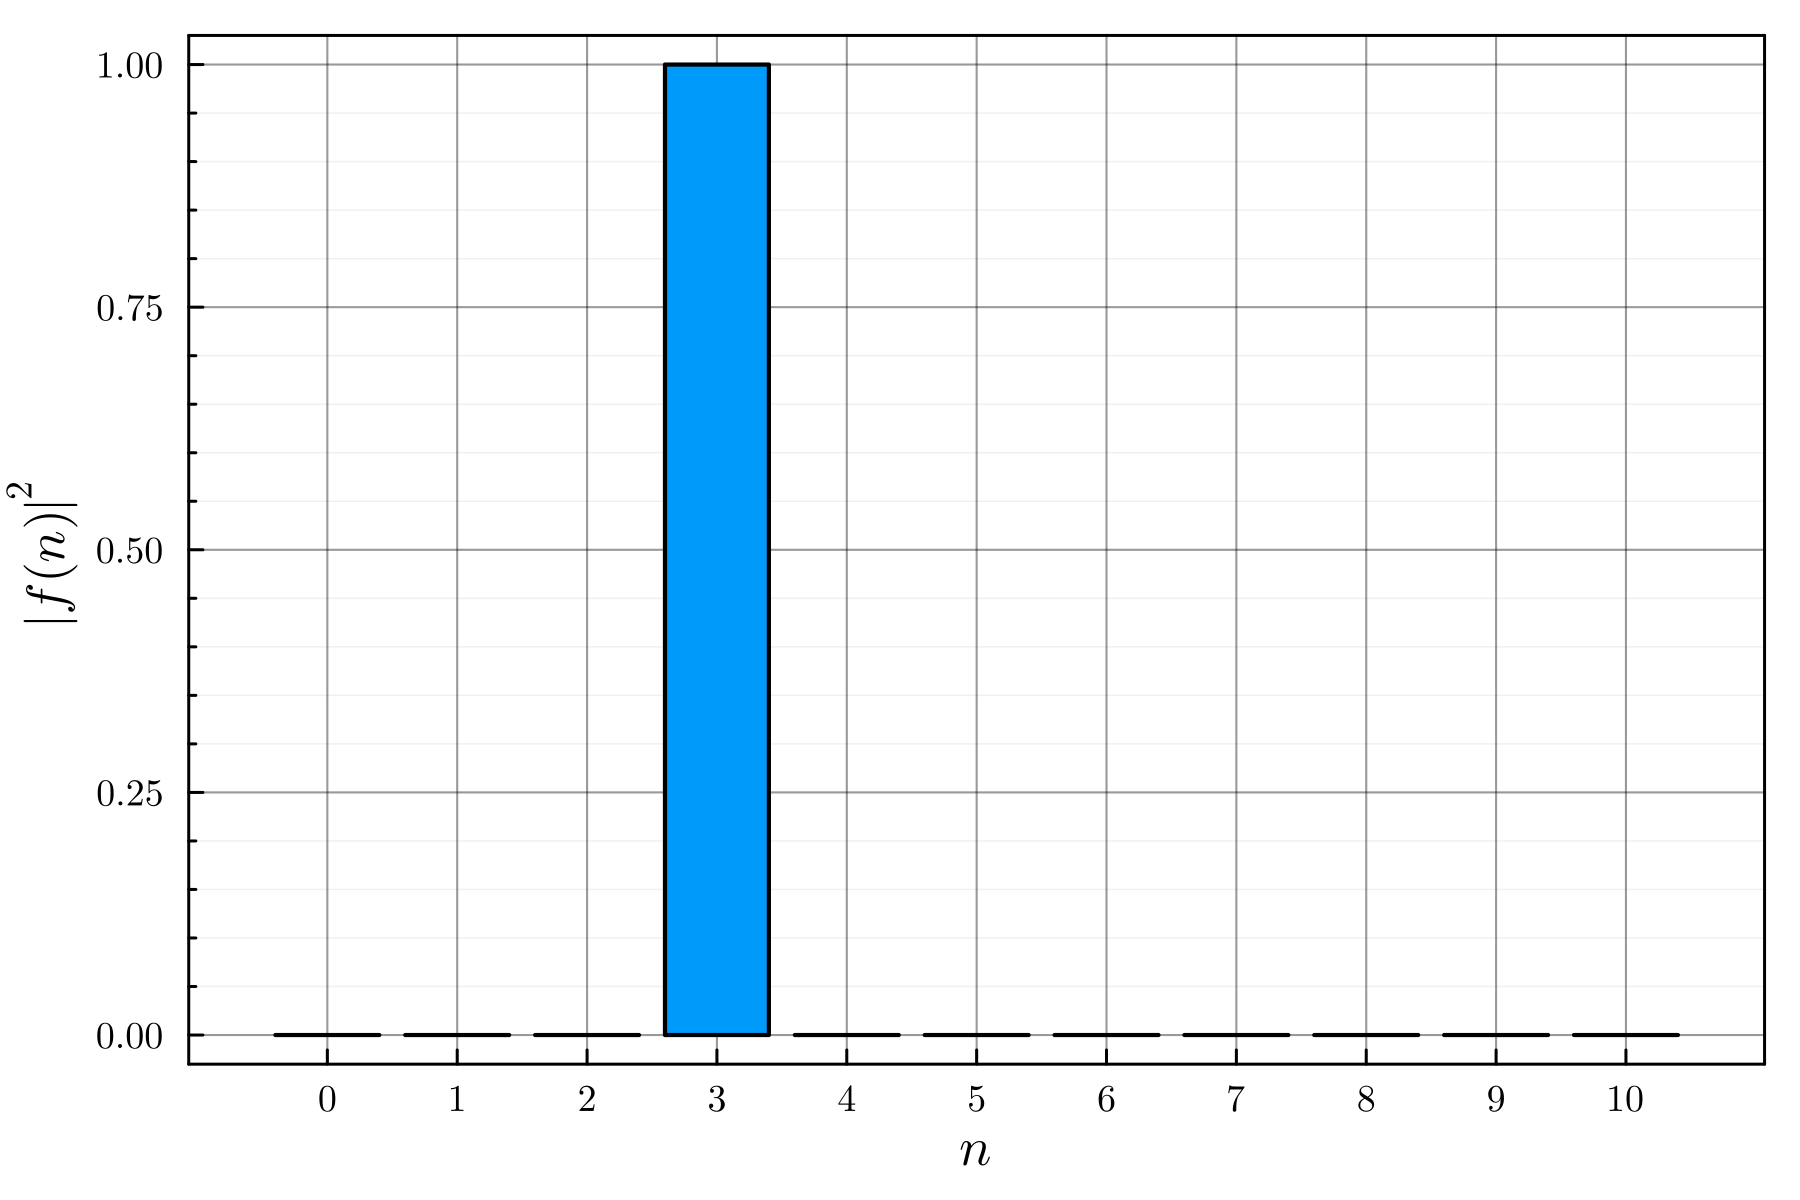
\includegraphics[width=\textwidth]{ch4/MI_dist.png}
        \caption{Mott insulator; $t = 0.01, \mu = 2.5$, $U = 1$}
        \label{fig:mi_dist}
    \end{subfigure}
    \hspace{1em}  %\hfill
    \begin{subfigure}[b]{0.48\textwidth}
        \centering
        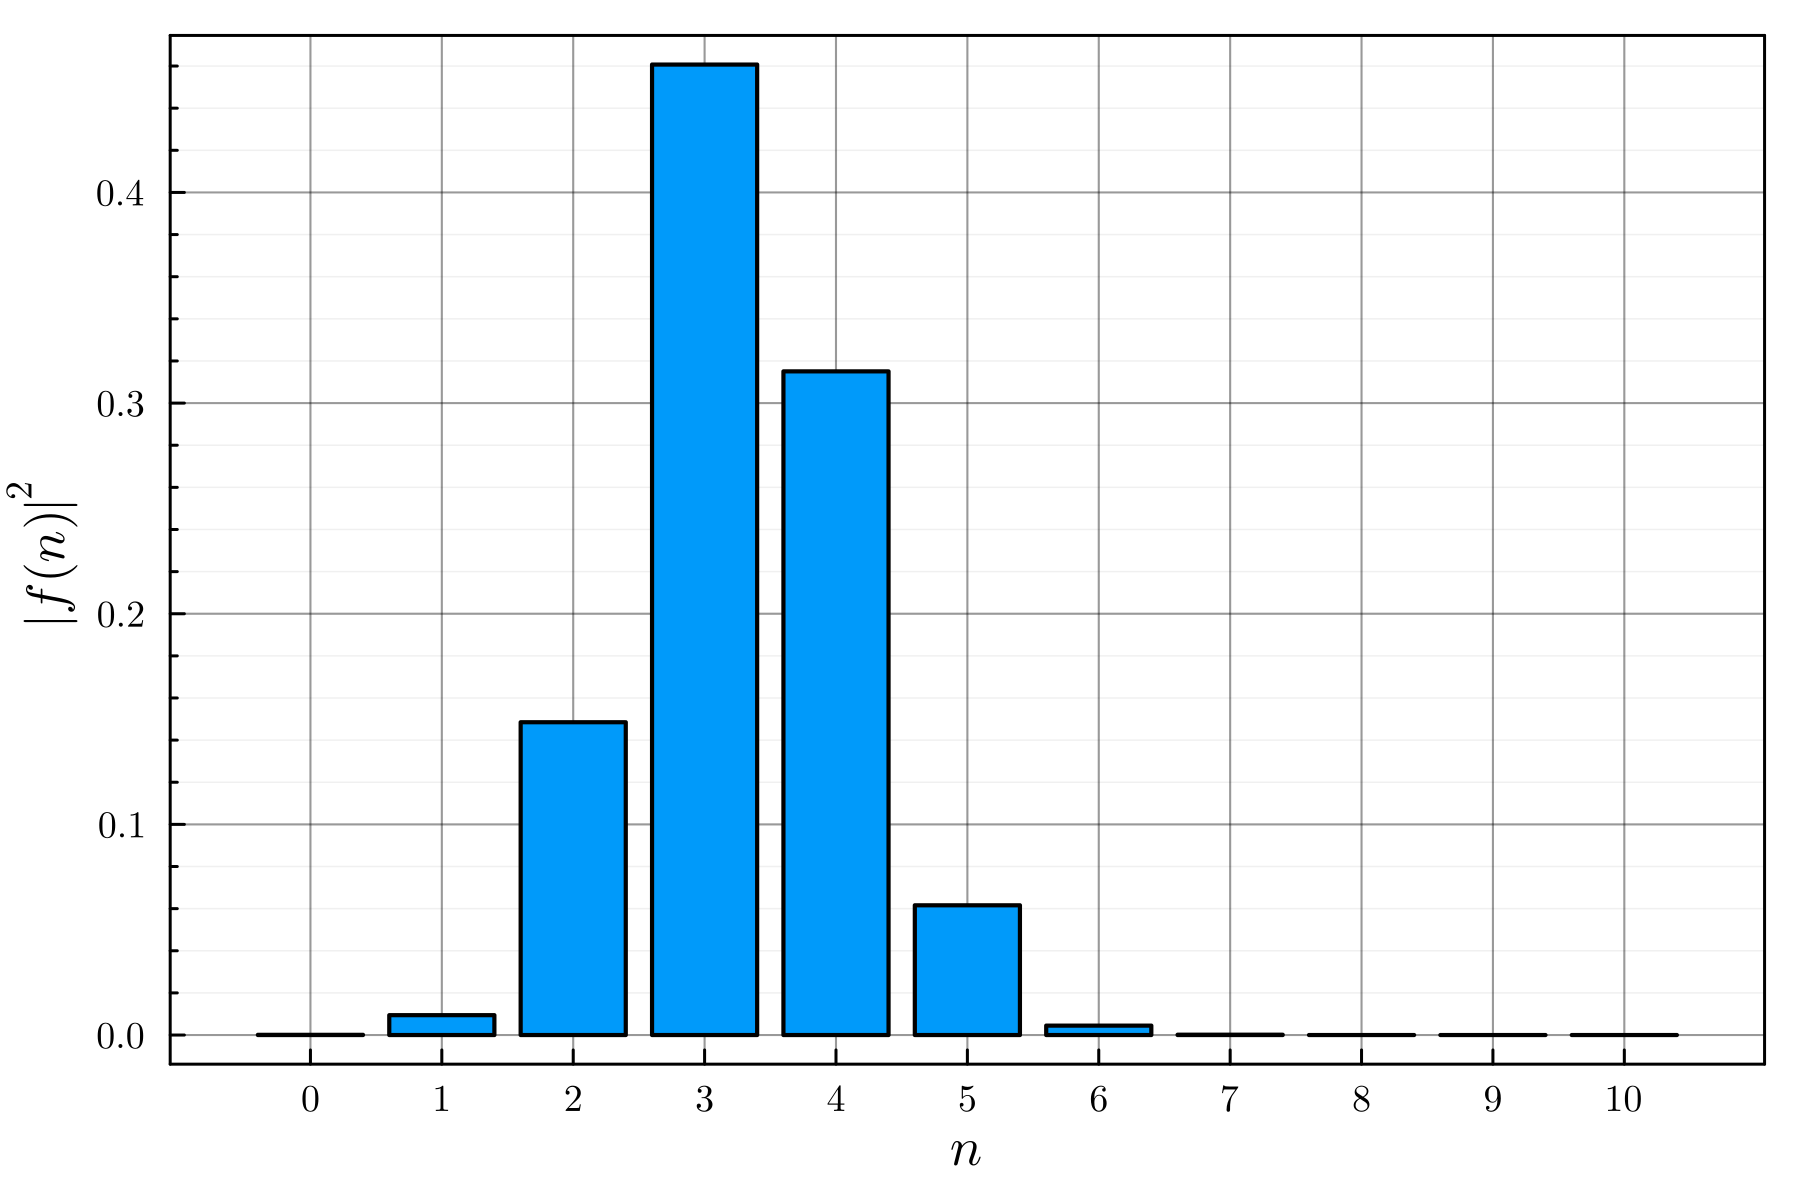
\includegraphics[width=\textwidth]{ch4/SF_dist.png}
        \caption{Superfluid; $t = 0.2, \mu = 2.5$, $U = 1$}
        \label{fig:sf_dist}
    \end{subfigure}
    \caption{Distribution of co-efficients in Fock basis}
    \label{fig:dists}
\end{figure}
%%% FIG %%%
\FloatBarrier \!\!\!\!\!\!\!\!\!\!\!

Solving the mean-field Hamiltonian for various parameter choices results in two distinct phases as seen in Fig. \ref{fig:dists}. The Mott insulator phase is captured as a pure Fock state with fixed occupation number on each lattice site. On the other hand, the superfluid phase is captured as a product of coherent states, which is a well-known means of describing BECs\cite{leggett2008, annett2003}. This can also be understood as the ground state picking up a random phase, $e^{i\theta}$, due to spontaneous breaking of the $U(1)$ symmetry. Further, the idea of particle number conservation can be loosely recovered by considering the thermodynamic limit wherein $\sqrt{\langle \delta n^2 \rangle}/\langle n \rangle \to 0$ as $N, M \to \infty$. In case this explanation is unsatisfactory, there is a way to formulate this scheme without breaking number conservation\cite{leggett2008}, but the analysis becomes far more cumbersome.
\vspace{0.5cm}\\
Now that we have confirmed that the ground state can admit these phases, we require an order parameter to distinguish them. A simple quantity presents itself by considering the definition of off-diagonal long-range order from Eq. \eqref{eq:odlro} as a means of identifying BECs.
\begin{equation}
    \lim_{|i-j| \to \infty} \langle a_i^{\dagger}a_j\rangle = \lim_{|i-j| \to \infty} \langle a_i^{\dagger}\rangle \langle a_j\rangle = \Psi_i^* \Psi_j = |\Psi|^2 \neq 0
\end{equation}
Note that such a decoupling is only valid at the mean-field level. We can clearly see now that the idea of spontaneous $U(1)$ symmetry breaking is captured by this result. Thus, we can use the mean-field parameter $\Psi$ as the superfluid order parameter as well.
\vspace{0.5cm}\\
The phase diagram can now be naively generated by computing the ground-state solution and hence the order parameter over a grid of $\mu/U$ and $t/U$ values.

\begin{figure}[!htb]
    \centering
    \begin{subfigure}[b]{0.45\textwidth}  %keep total sum <1 to show in same line
        \centering
        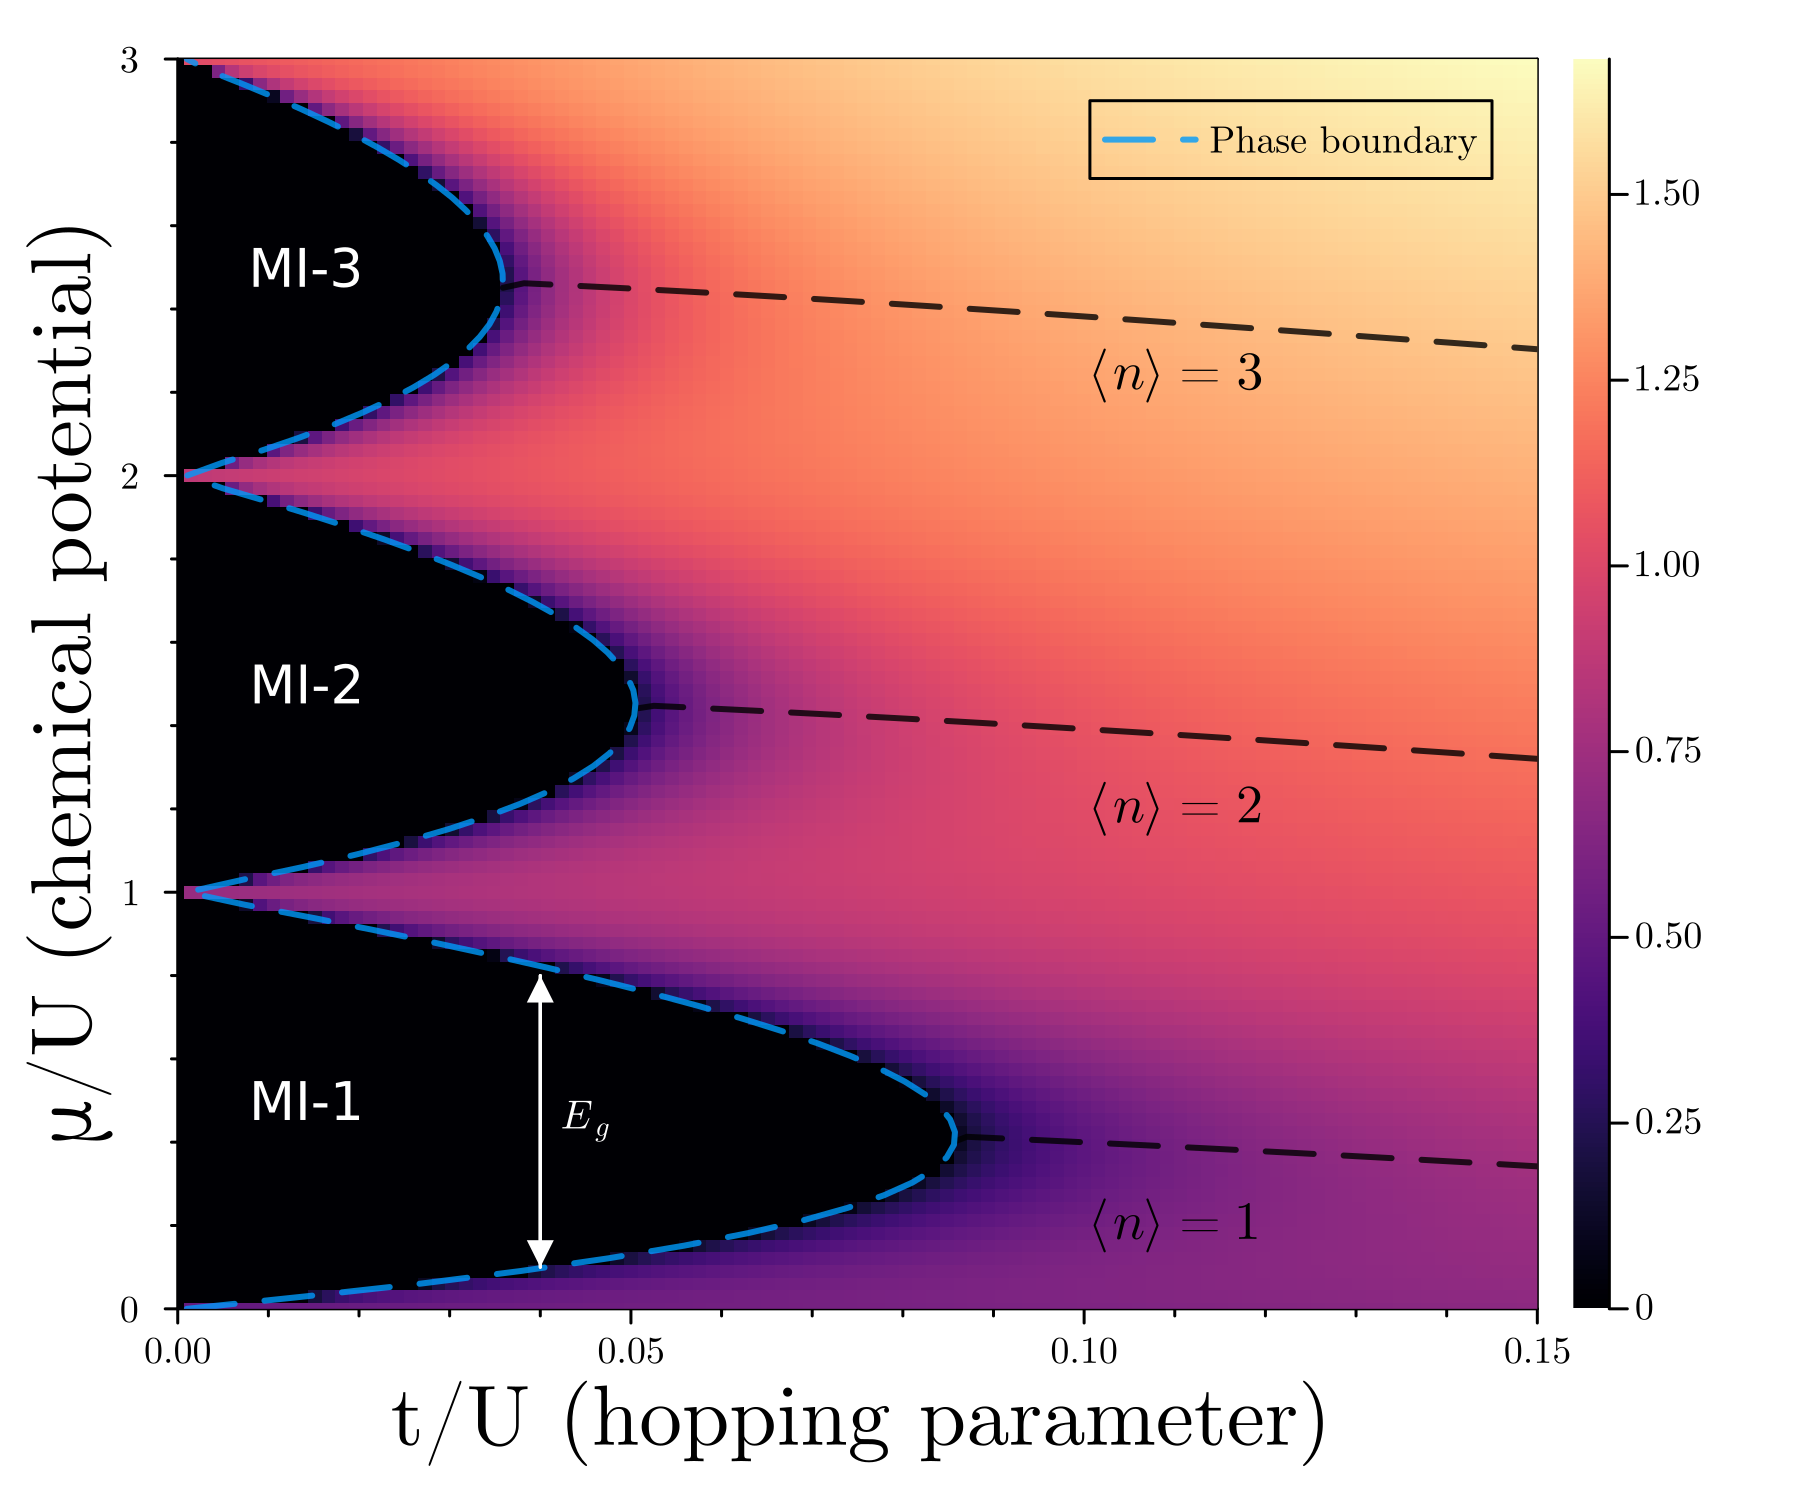
\includegraphics[width=\textwidth]{ch4/phase_diagram_op.png}
        \caption{Order parameter, $\langle a \rangle$}
        \label{fig:mft_pd}
    \end{subfigure}
    \hspace{1em}  %\hfill
    \begin{subfigure}[b]{0.45\textwidth}
        \centering
        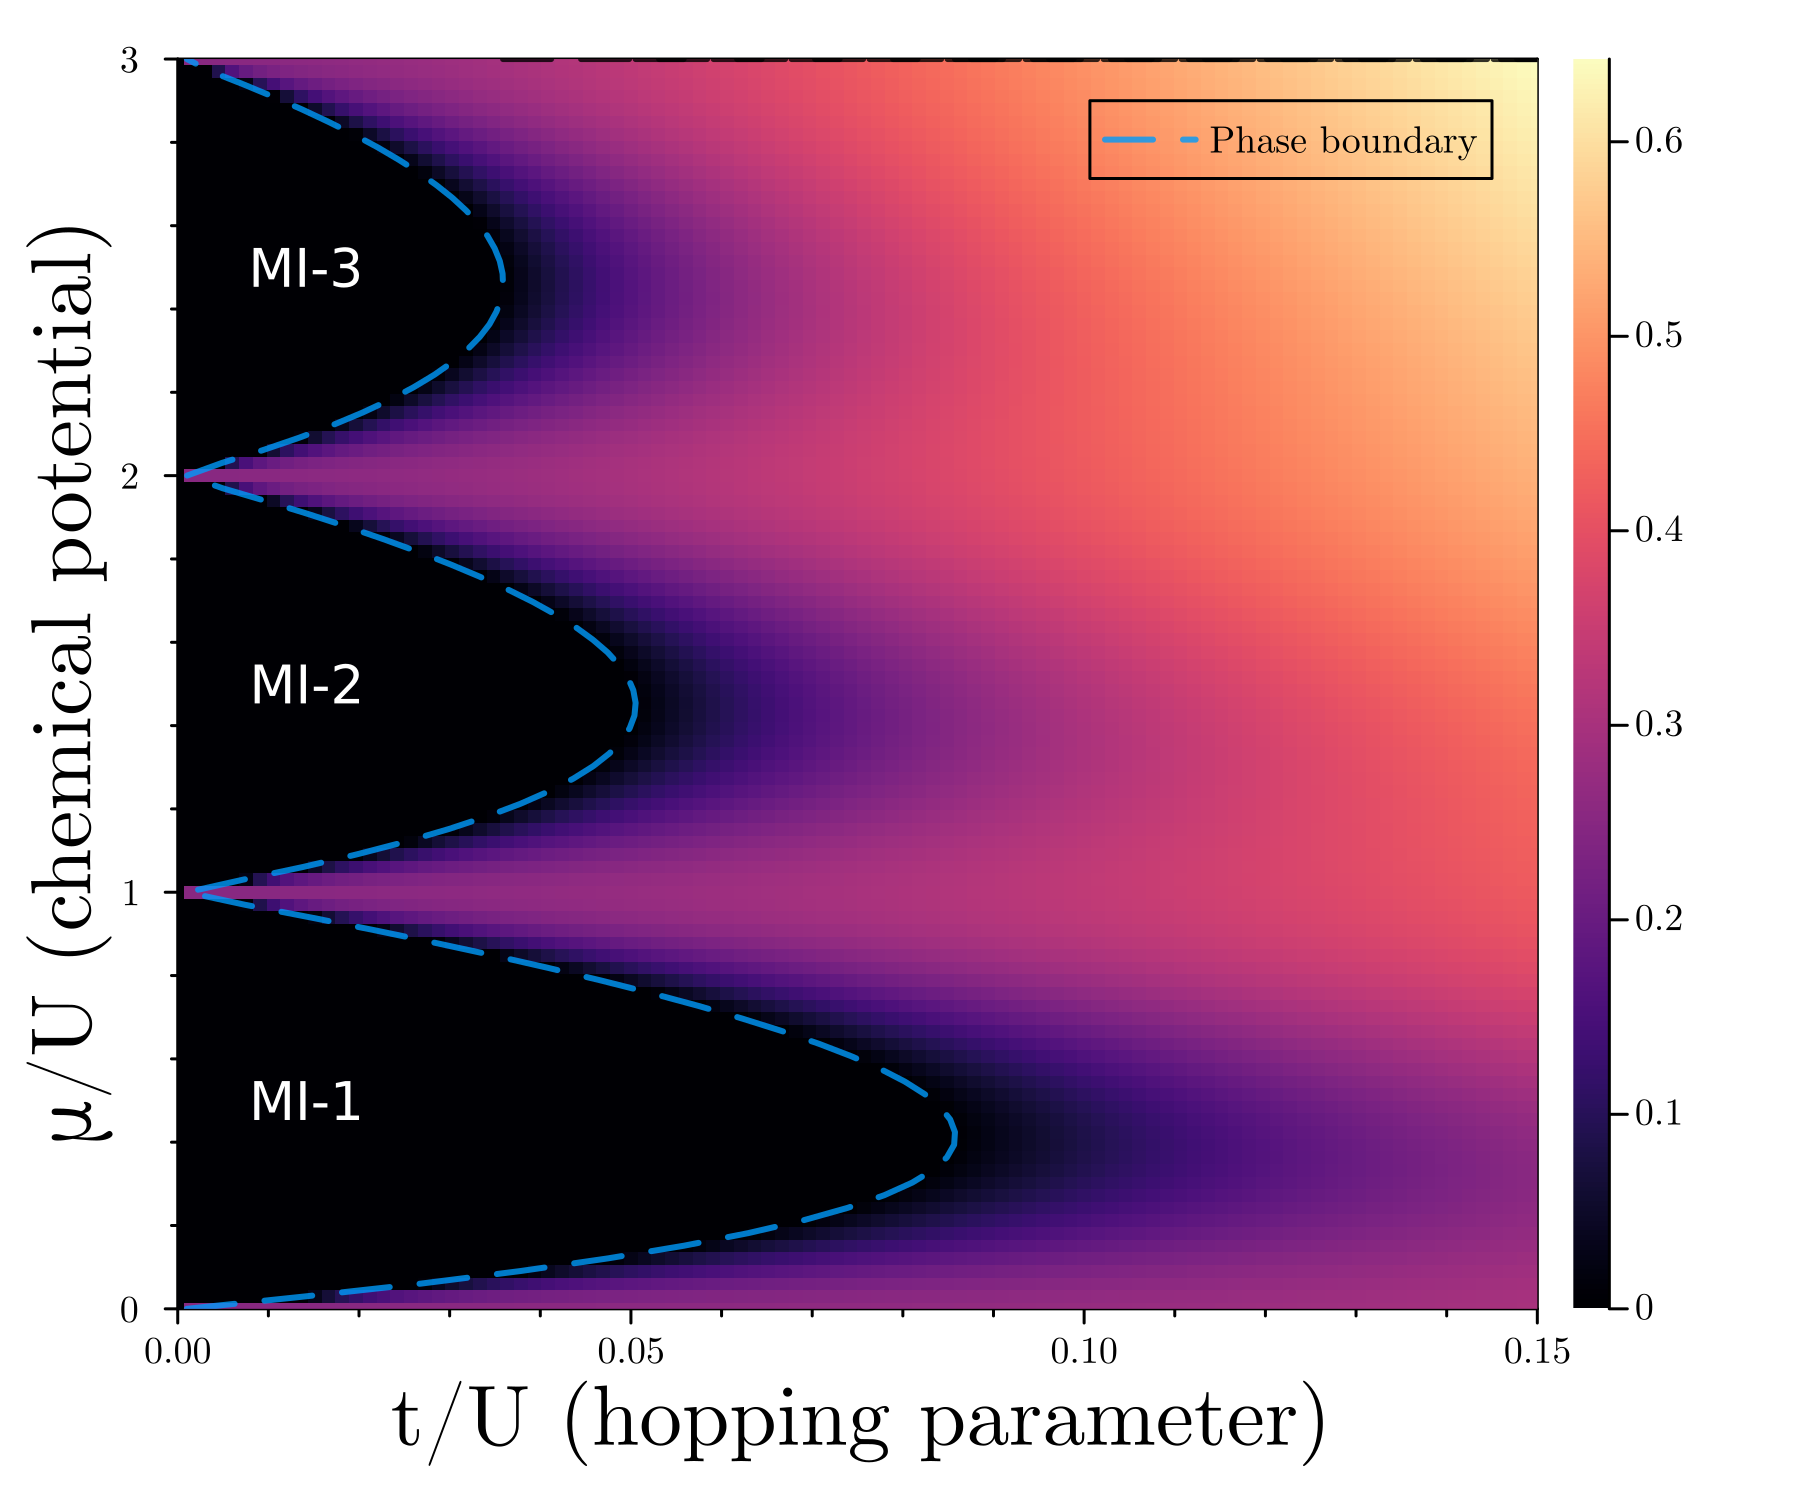
\includegraphics[width=\textwidth]{ch4/phase_diagram_nvar.png}
        \caption{Occupation number variance, $\langle \delta n^2 \rangle$}
        \label{fig:mft_occvar}
    \end{subfigure}
    \caption{1D Mean-field phase diagram}
    \label{}
\end{figure}
%%% FIG %%%
\FloatBarrier \!\!\!\!\!\!\!\!\!\!\!

A clean phase diagram is obtained in Fig \ref{fig:mft_pd}, where the Mott insulator phase manifests as lobes in the $t-\mu$ plane. We also note from Fig. \ref{fig:mft_occvar} that the occupation number variance serves as an equally valid order parameter, giving us the same phase boundary (although the heatmap is a bit misleading). We can now get further insight into the nature of the Mott lobes by plotting the average occupation number.
%%% FIG %%%
\begin{figure}[!htb]
    \centering
    \begin{subfigure}[b]{0.43\textwidth}  %keep total sum <1 to show in same line
        \centering
        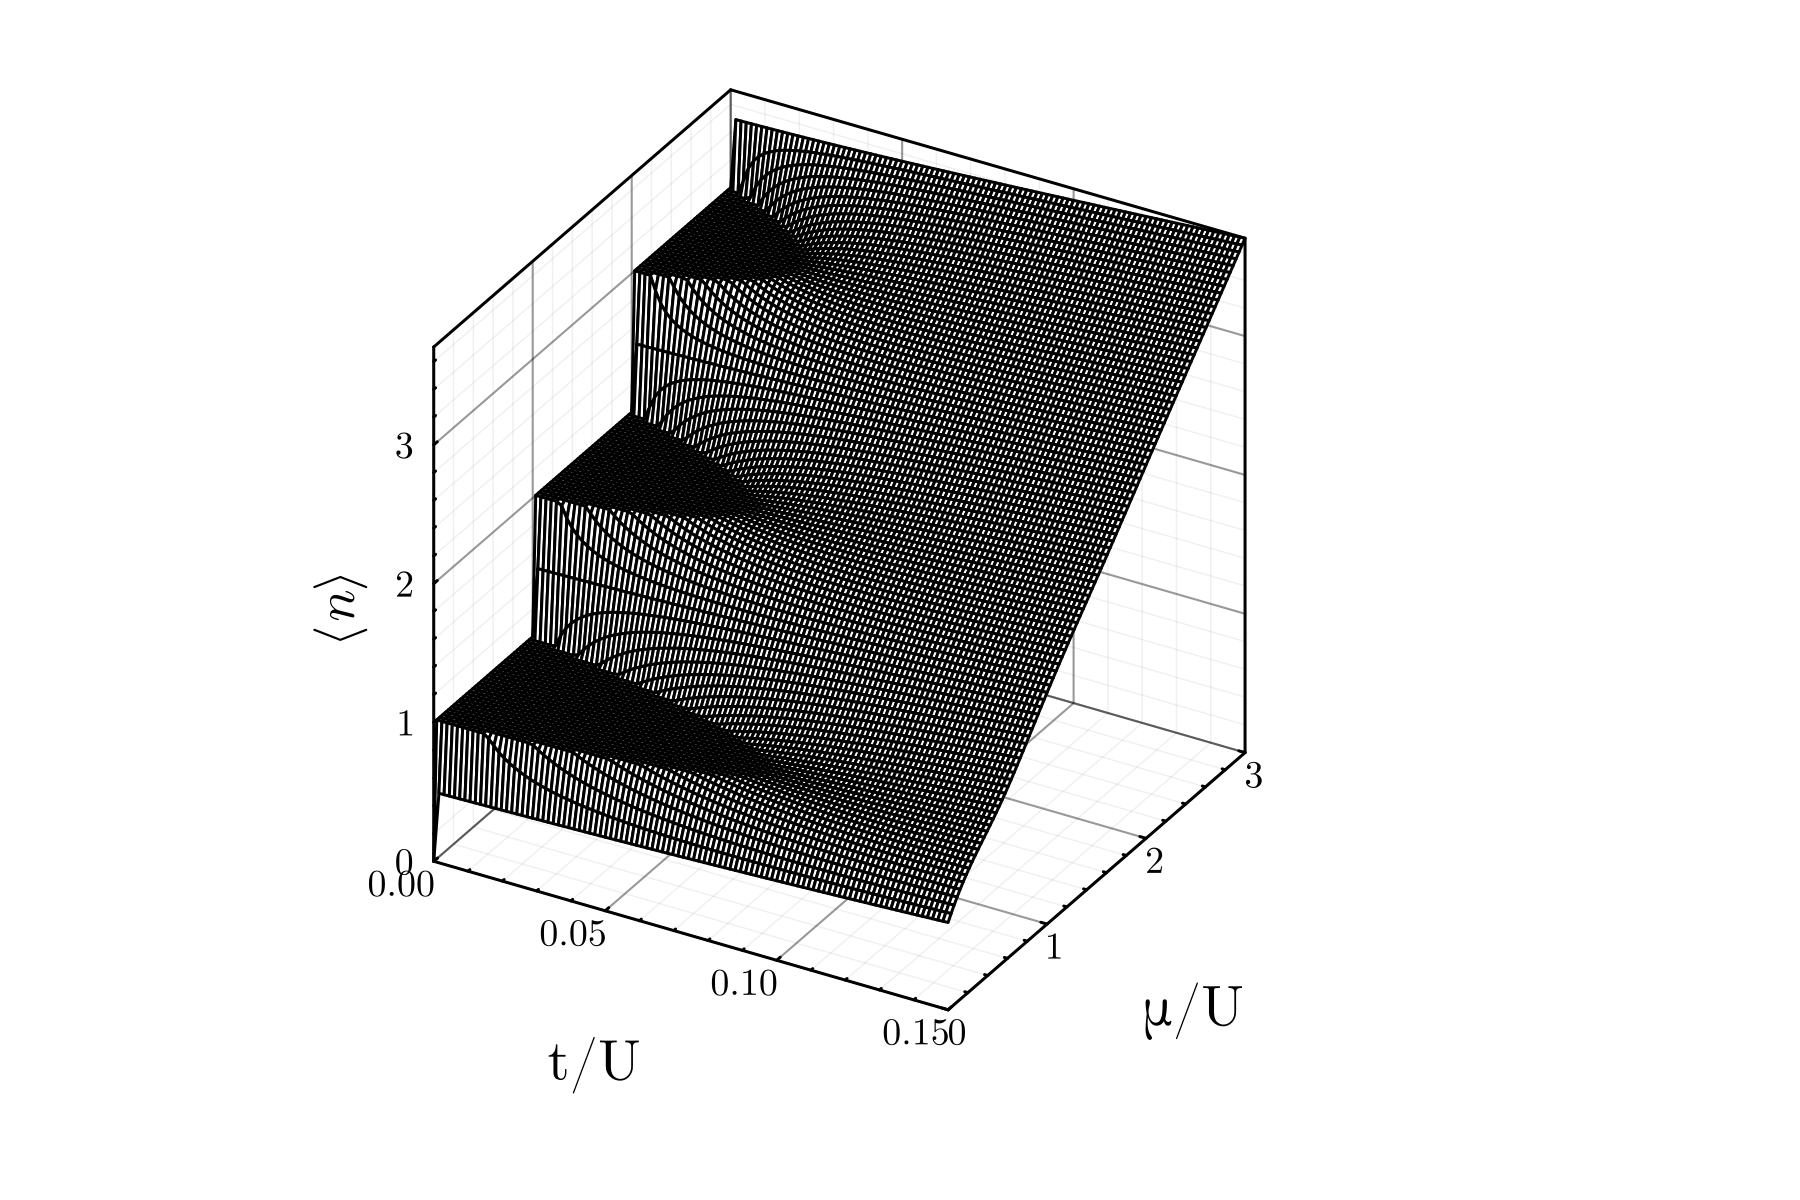
\includegraphics[width=\textwidth]{ch4/num_particles.png}
        \caption{Average occupation number}
    \end{subfigure}
    \hspace{1em}  %\hfill
    \begin{subfigure}[b]{0.4\textwidth}
        \centering
        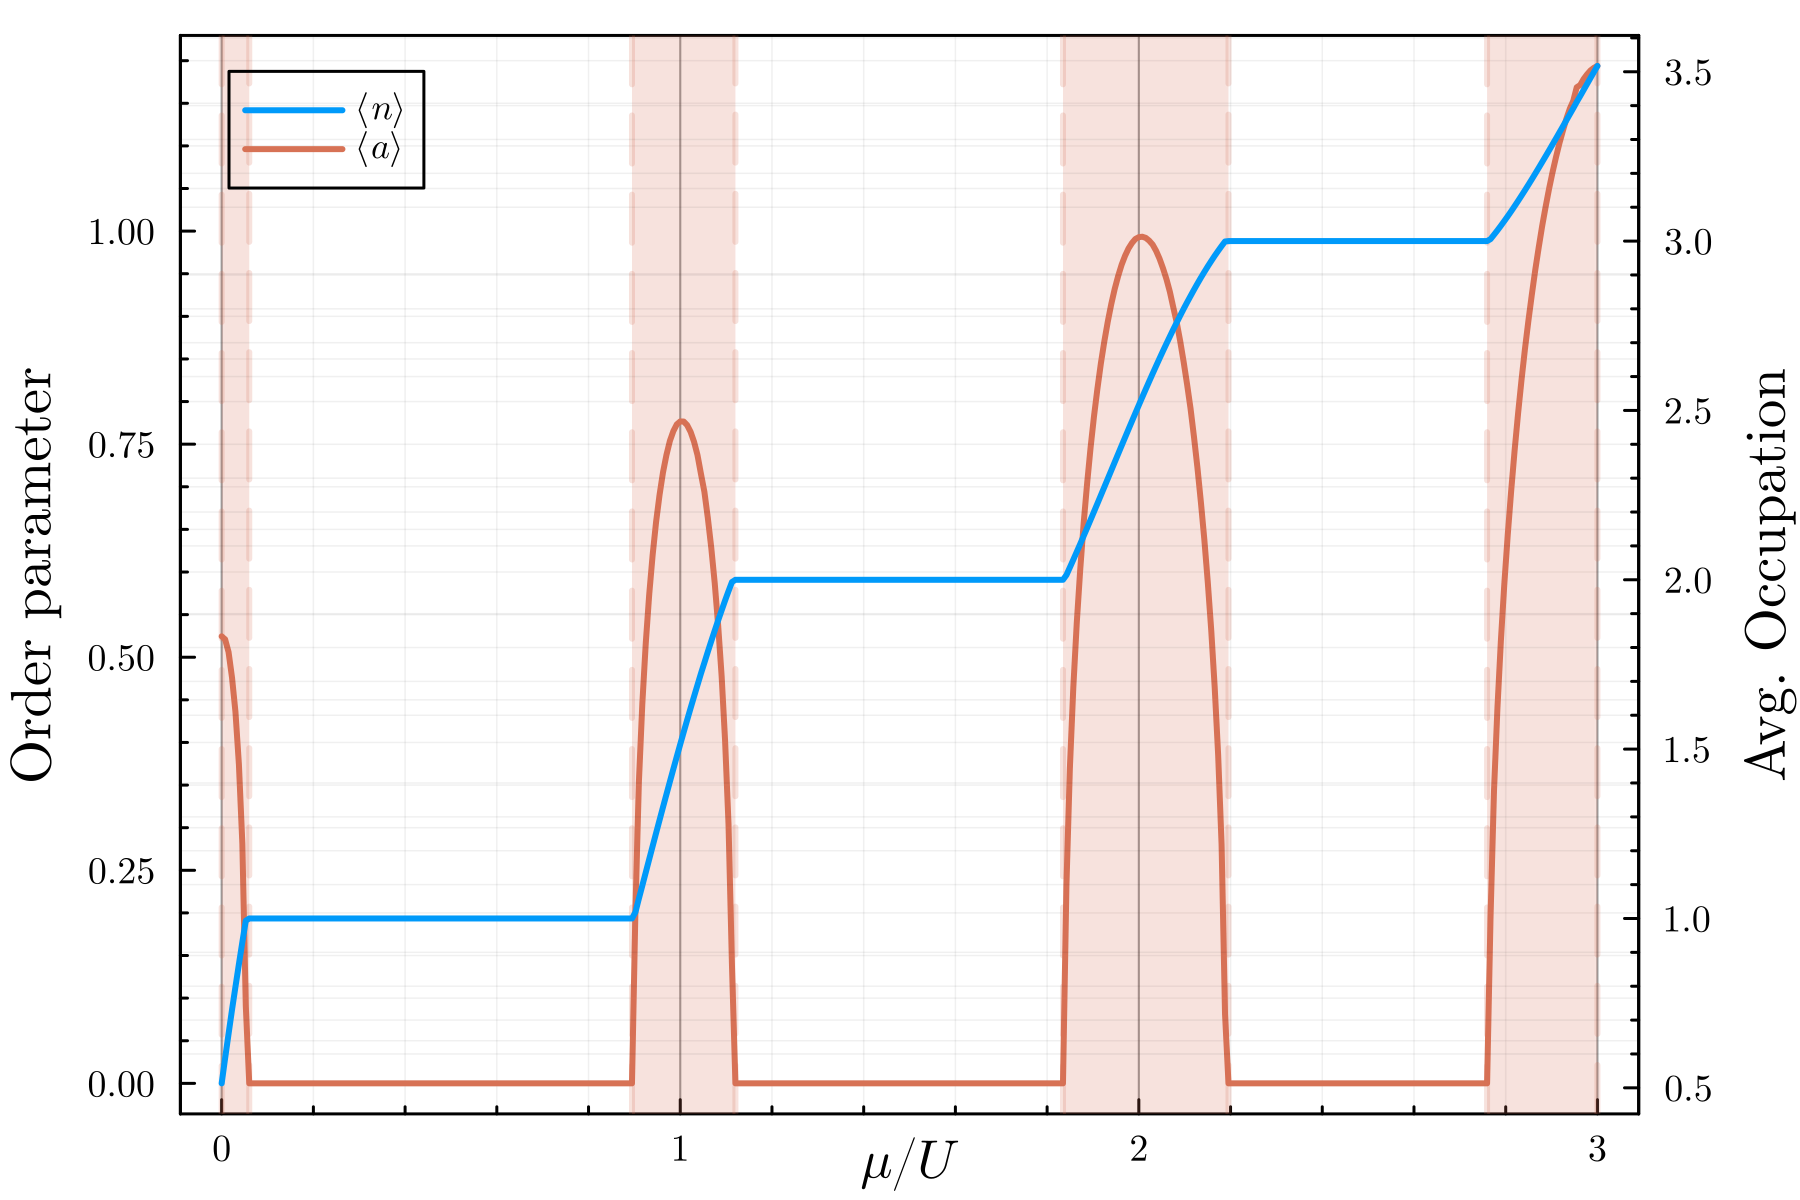
\includegraphics[width=\textwidth]{ch4/MFT_section.png}
        \caption{Cross-section at $t = 0.024$}
    \end{subfigure}
    \caption{Distinguishing phases using the average occupation}
    \label{fig:mft_avg_occ}
\end{figure}
%%% FIG %%%
\FloatBarrier \!\!\!\!\!\!\!\!\!\!\!

As expected, Fig. \ref{fig:mft_avg_occ} shows the existence of integer occupation plateaus corresponding to the points where the order parameter vanishes in the phase diagram. As the chemical potential is increased, there is a sudden jump to the next Mott lobe admitting one more boson per lattice site. Further, for a given point inside a Mott lobe, the vertical distance to the lower (upper) arm denotes the energy required to excite a hole (particle), thus supporting the fact that the Mott insulator is indeed a gapped phase. 
\vspace{0.5cm}\\
We also note that the MI-SF transition is second order since the order parameter changes continuously across the boundary. As a result, one can also perturbatively treat the hopping term in Eq. \ref{eq:mft} to directly obtain an analytic expression for the phase boundary\cite{Cubela19}. This matches exactly with our numerical results since the perturbative term is proportional to $\Psi$, which can be chosen to be arbitrarily small near the phase boundary. 

\subsection{A better technique}
Although the grid-based approach gives us a qualitative idea of the phase diagram, the accuracy of the phase boundary is limited by the discretization of the grid. However, the fact that there is only a single transition along $t$ for a fixed value of $\mu$ lets us utilize a bisection method to determine the transition point, $t_c$. Performing this for a grid of values of $\mu$ gives us the phase boundary such that the error falls as $1/2^n$ for $n$ bisections.
\vspace{0.5cm}\\
But we can do even better! To utilize the bisection method, at any given point we only require the information of the ground state phase, i.e, the rest of the information contained in the ground-state is unnecessary. One approach could be to directly check if $\Psi = 0$ is a fixed point of the self-consistency function in Eq. \ref{eq:self_fn}. However, it turns out that $\Psi=0$ is \textit{always} a fixed point, but is unstable for the superfluid phase. In order to find another approach, let us analyze the nature of convergence of the self-consistent procedure.
%%% FIG %%%
\begin{figure}[!htb]
    \centering
    \begin{subfigure}[b]{0.45\textwidth}  %keep total sum <1 to show in same line
        \centering
        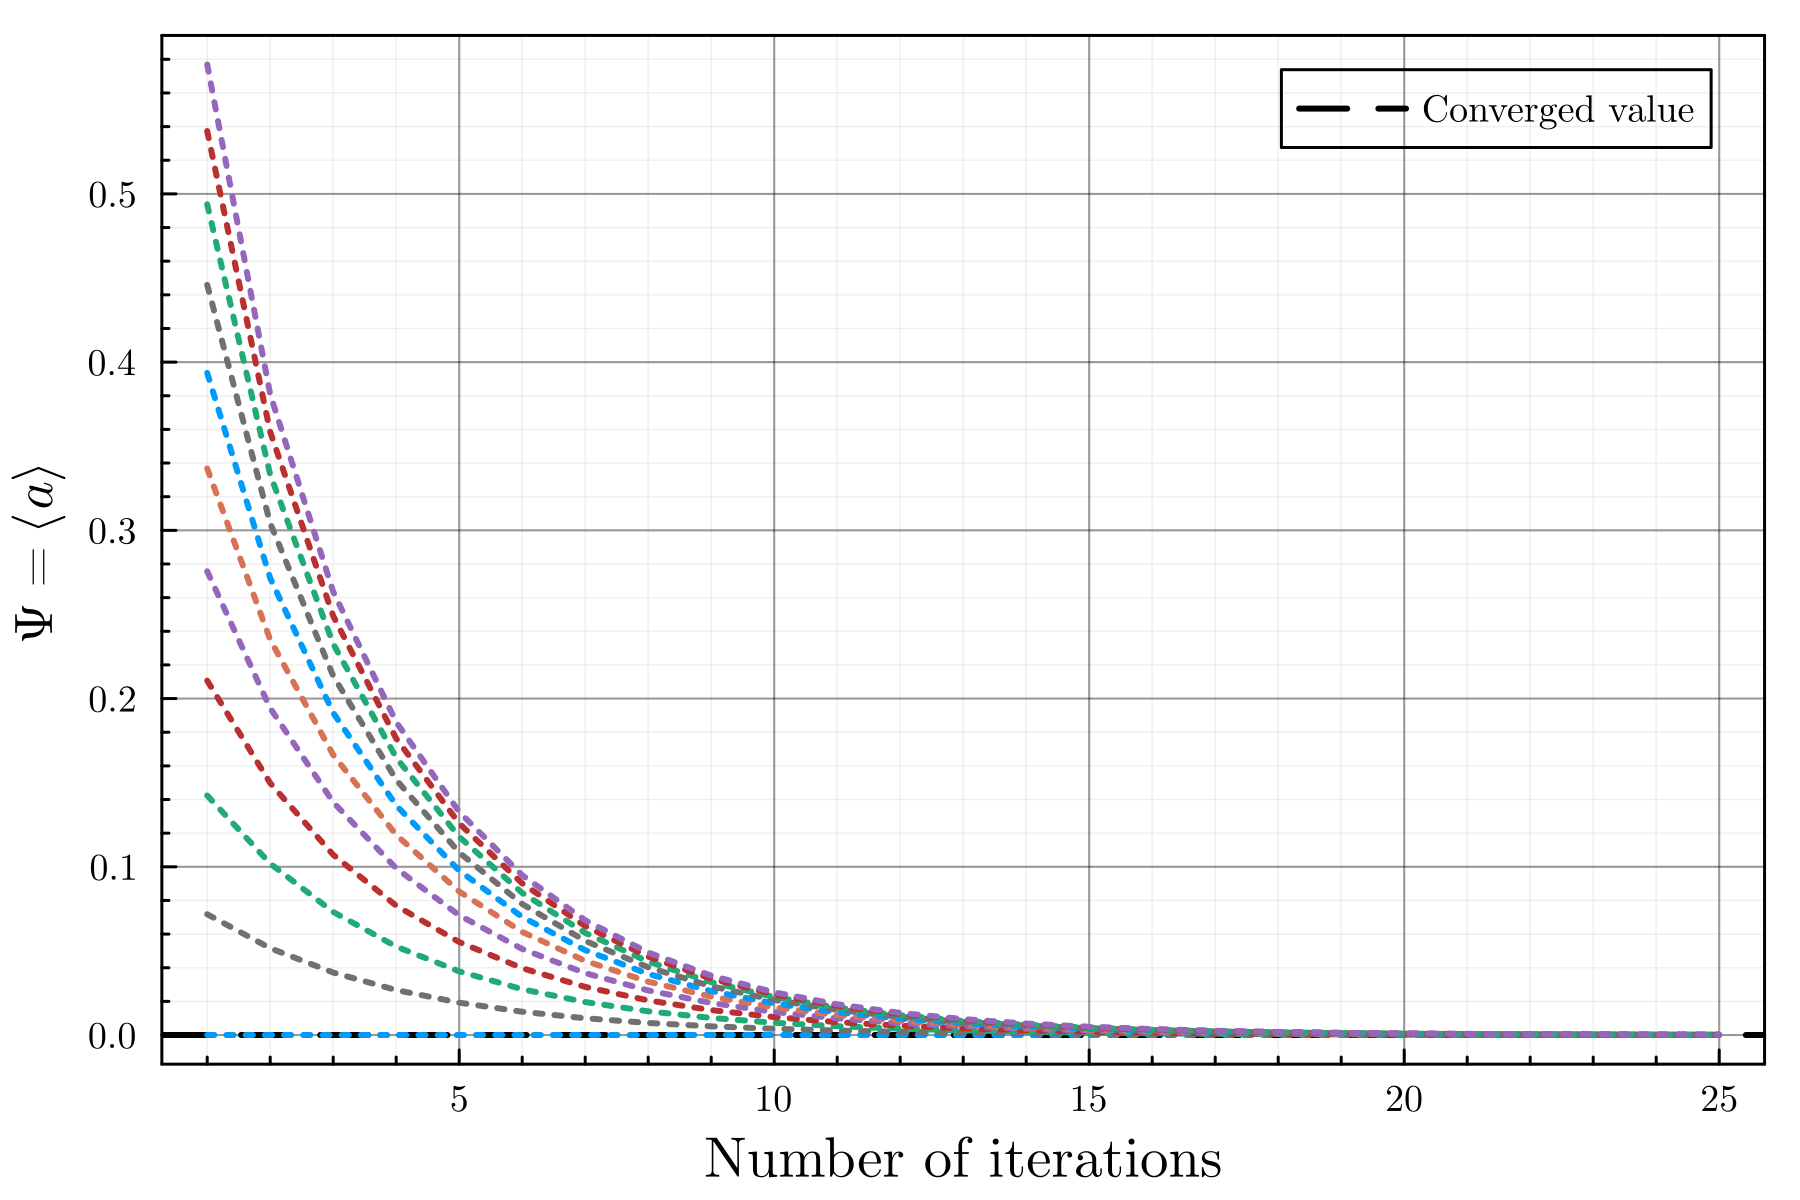
\includegraphics[width=\textwidth]{ch4/MI_converge.png}
        \caption{$t = 0.06, \mu = 0.5$}
    \end{subfigure}
    \hspace{1em}  %\hfill
    \begin{subfigure}[b]{0.45\textwidth}
        \centering
        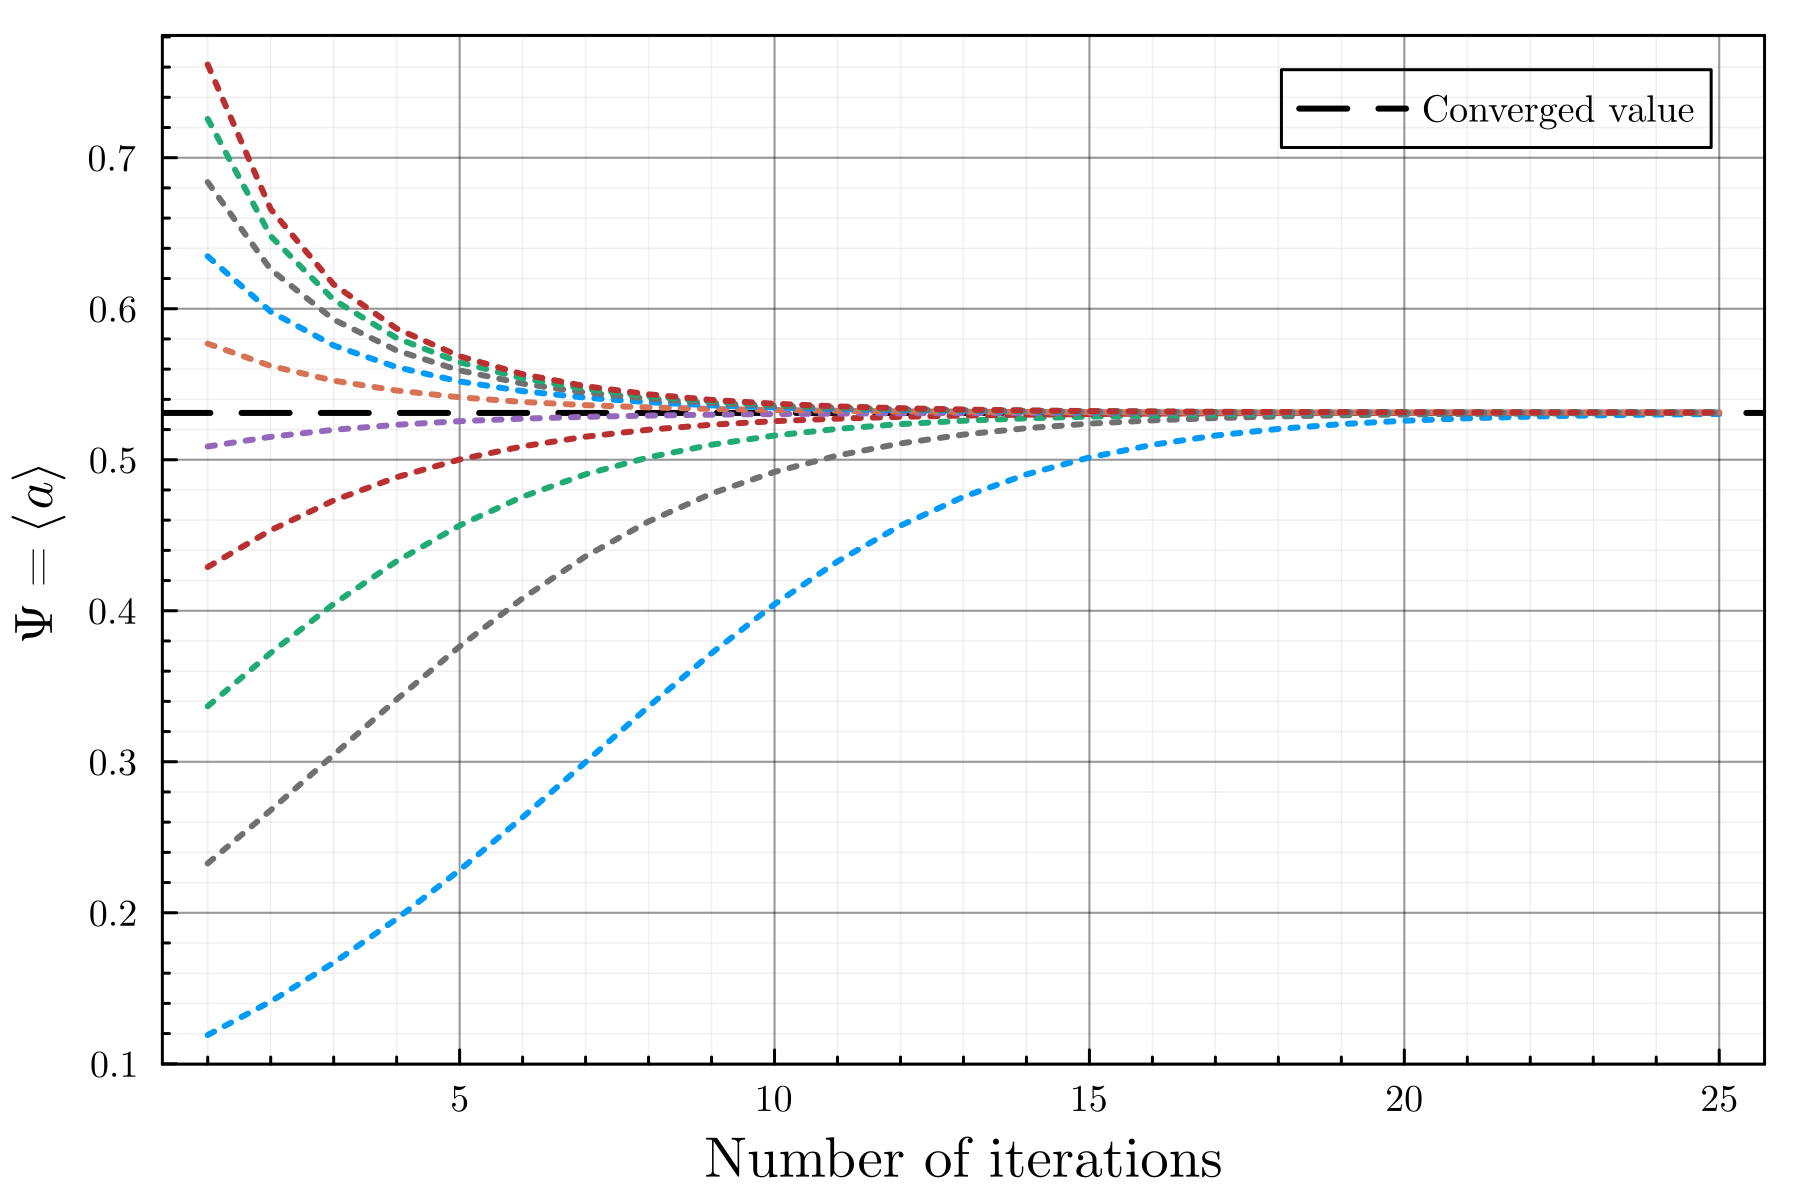
\includegraphics[width=\textwidth]{ch4/SF_converge.png}
        \caption{$t = 0.1, \mu = 0.5$}
    \end{subfigure}
    \caption{Monotonic convergence of self-consistency loop}
    \label{fig:self_consistent_converge}
\end{figure}
%%% FIG %%%
\FloatBarrier \!\!\!\!\!\!\!\!\!\!\!

It is apparent from Fig. \ref{fig:self_consistent_converge} that fixed-point iteration always monotonically converges to the stable fixed point for this system. This means that using a small initial guess such as $\Psi^{(0)} = 1\mathrm{e}{-9}$, we can determine whether $\Psi=0$ is a stable fixed point with a single iteration of the self-consistency loop\cite{Luhmann2013, Kho16}! 

%%% FIG %%%
\begin{figure}[!htb]
    \centering
    \begin{subfigure}[b]{0.75\textwidth}  %keep total sum <1 to show in same line
        \centering
        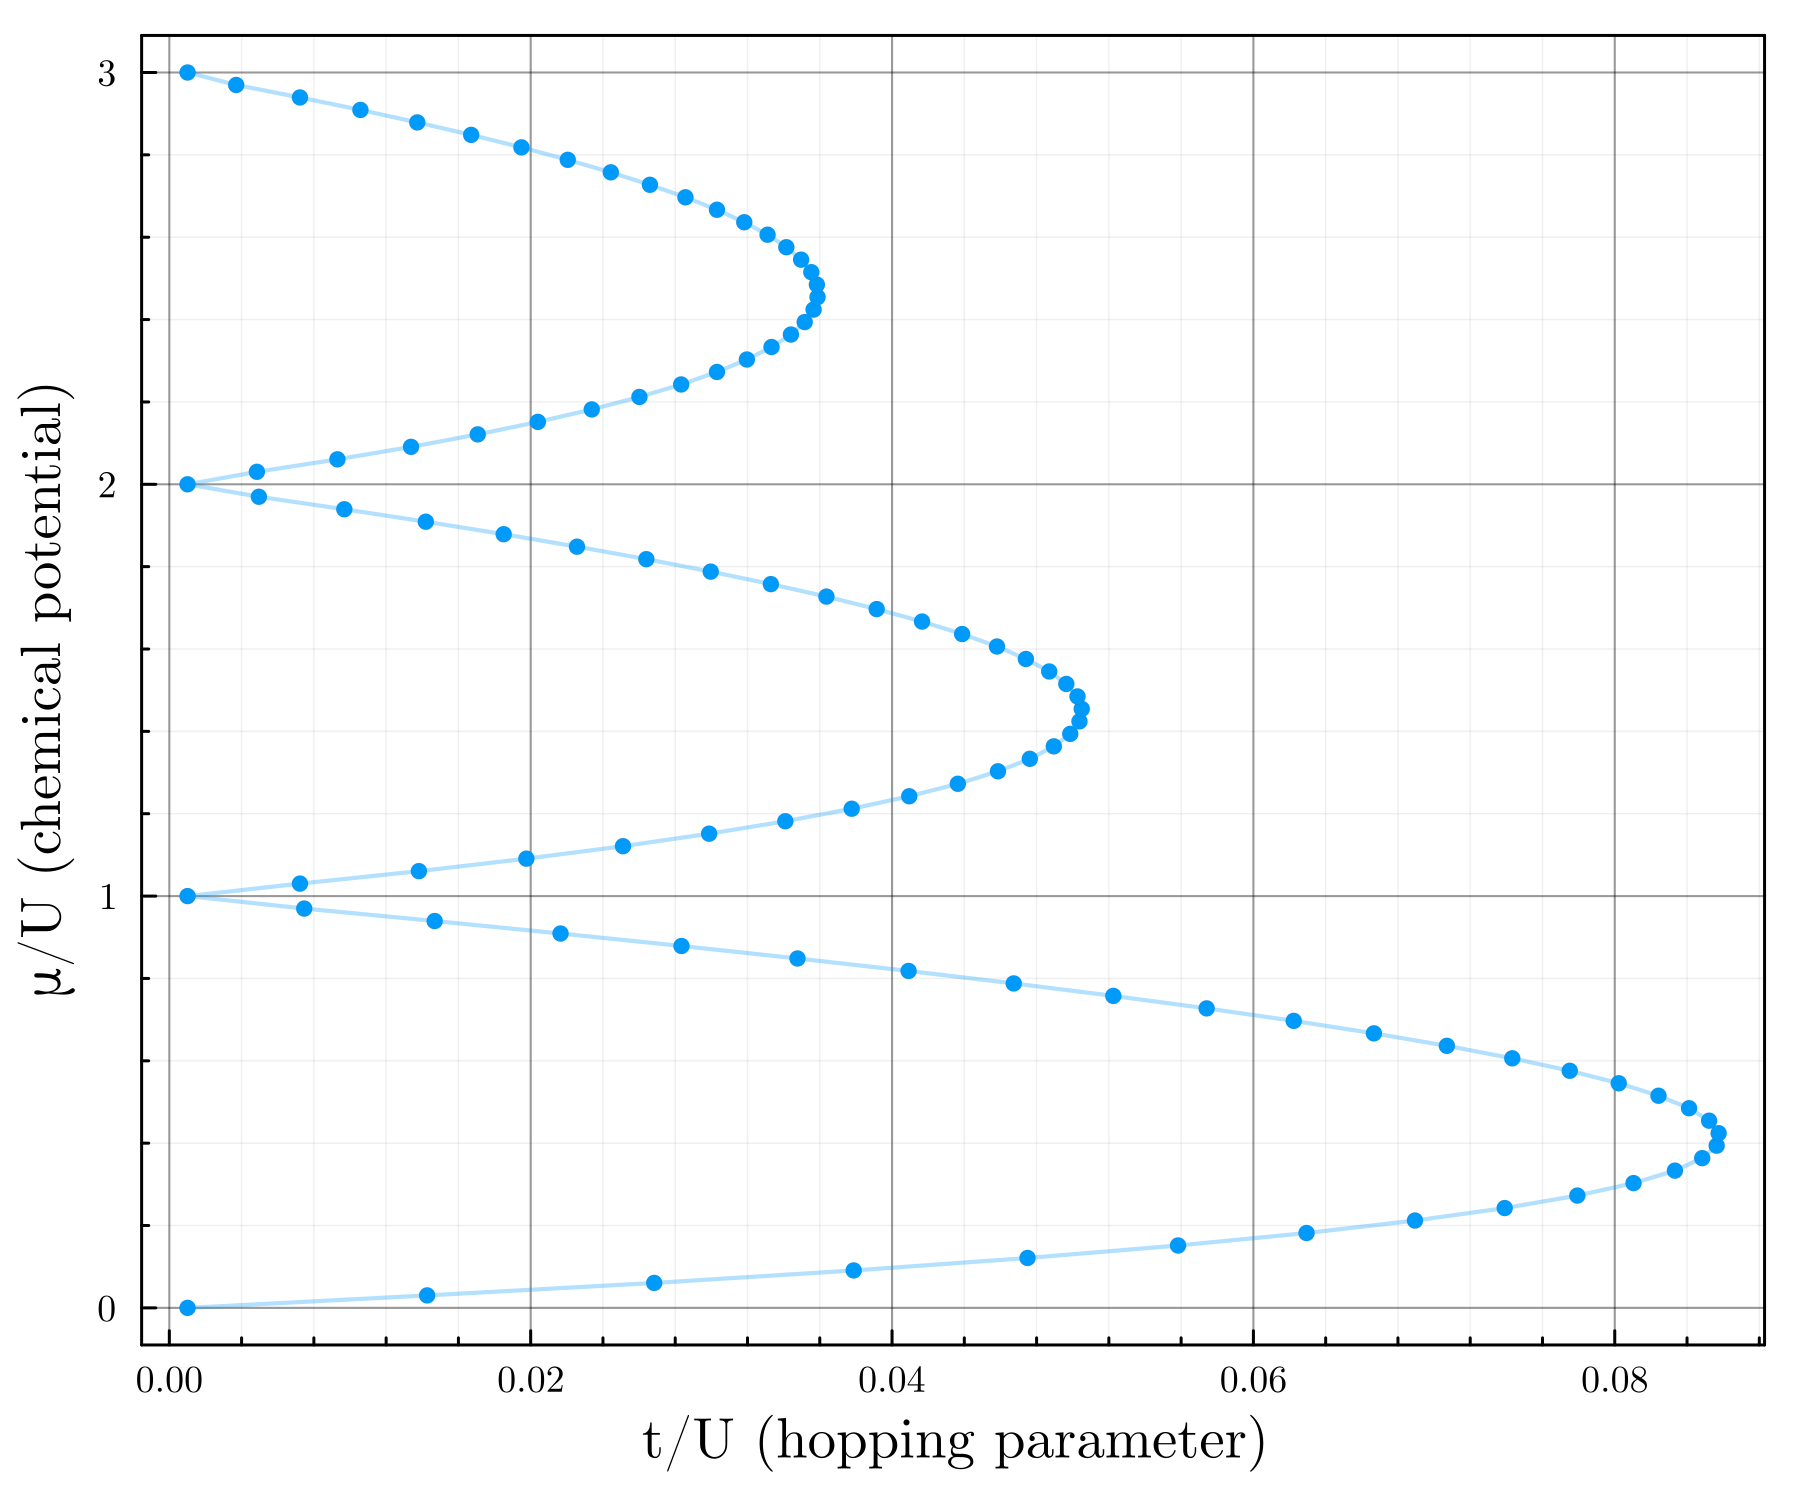
\includegraphics[width=\textwidth]{ch4/phase_diagram_bisection.png}
    \end{subfigure}
    \caption{1D Mean-field phase boundary determined by the bisection technique}
    \label{}
\end{figure}
%%% FIG %%%
\FloatBarrier \!\!\!\!\!\!\!\!\!\!\!

\subsection{Determining $n_{max}$}\label{sec:nmax}
Before wrapping up, we must tackle the issue of dealing with an infinite dimensional Hamiltonian. Truncating the Fock space at an arbitrary occupation number might seem like it fundamentally changes the model under consideration. The extreme limit of this is setting $n_{max} = 1$ corresponding to a system of hard-core bosons, and any higher truncation amounts to considering semi-hardcore bosons of sorts.
%%% FIG %%%
\begin{figure}[!htb]
    \centering
    \begin{subfigure}[b]{0.75\textwidth}  %keep total sum <1 to show in same line
        \centering
        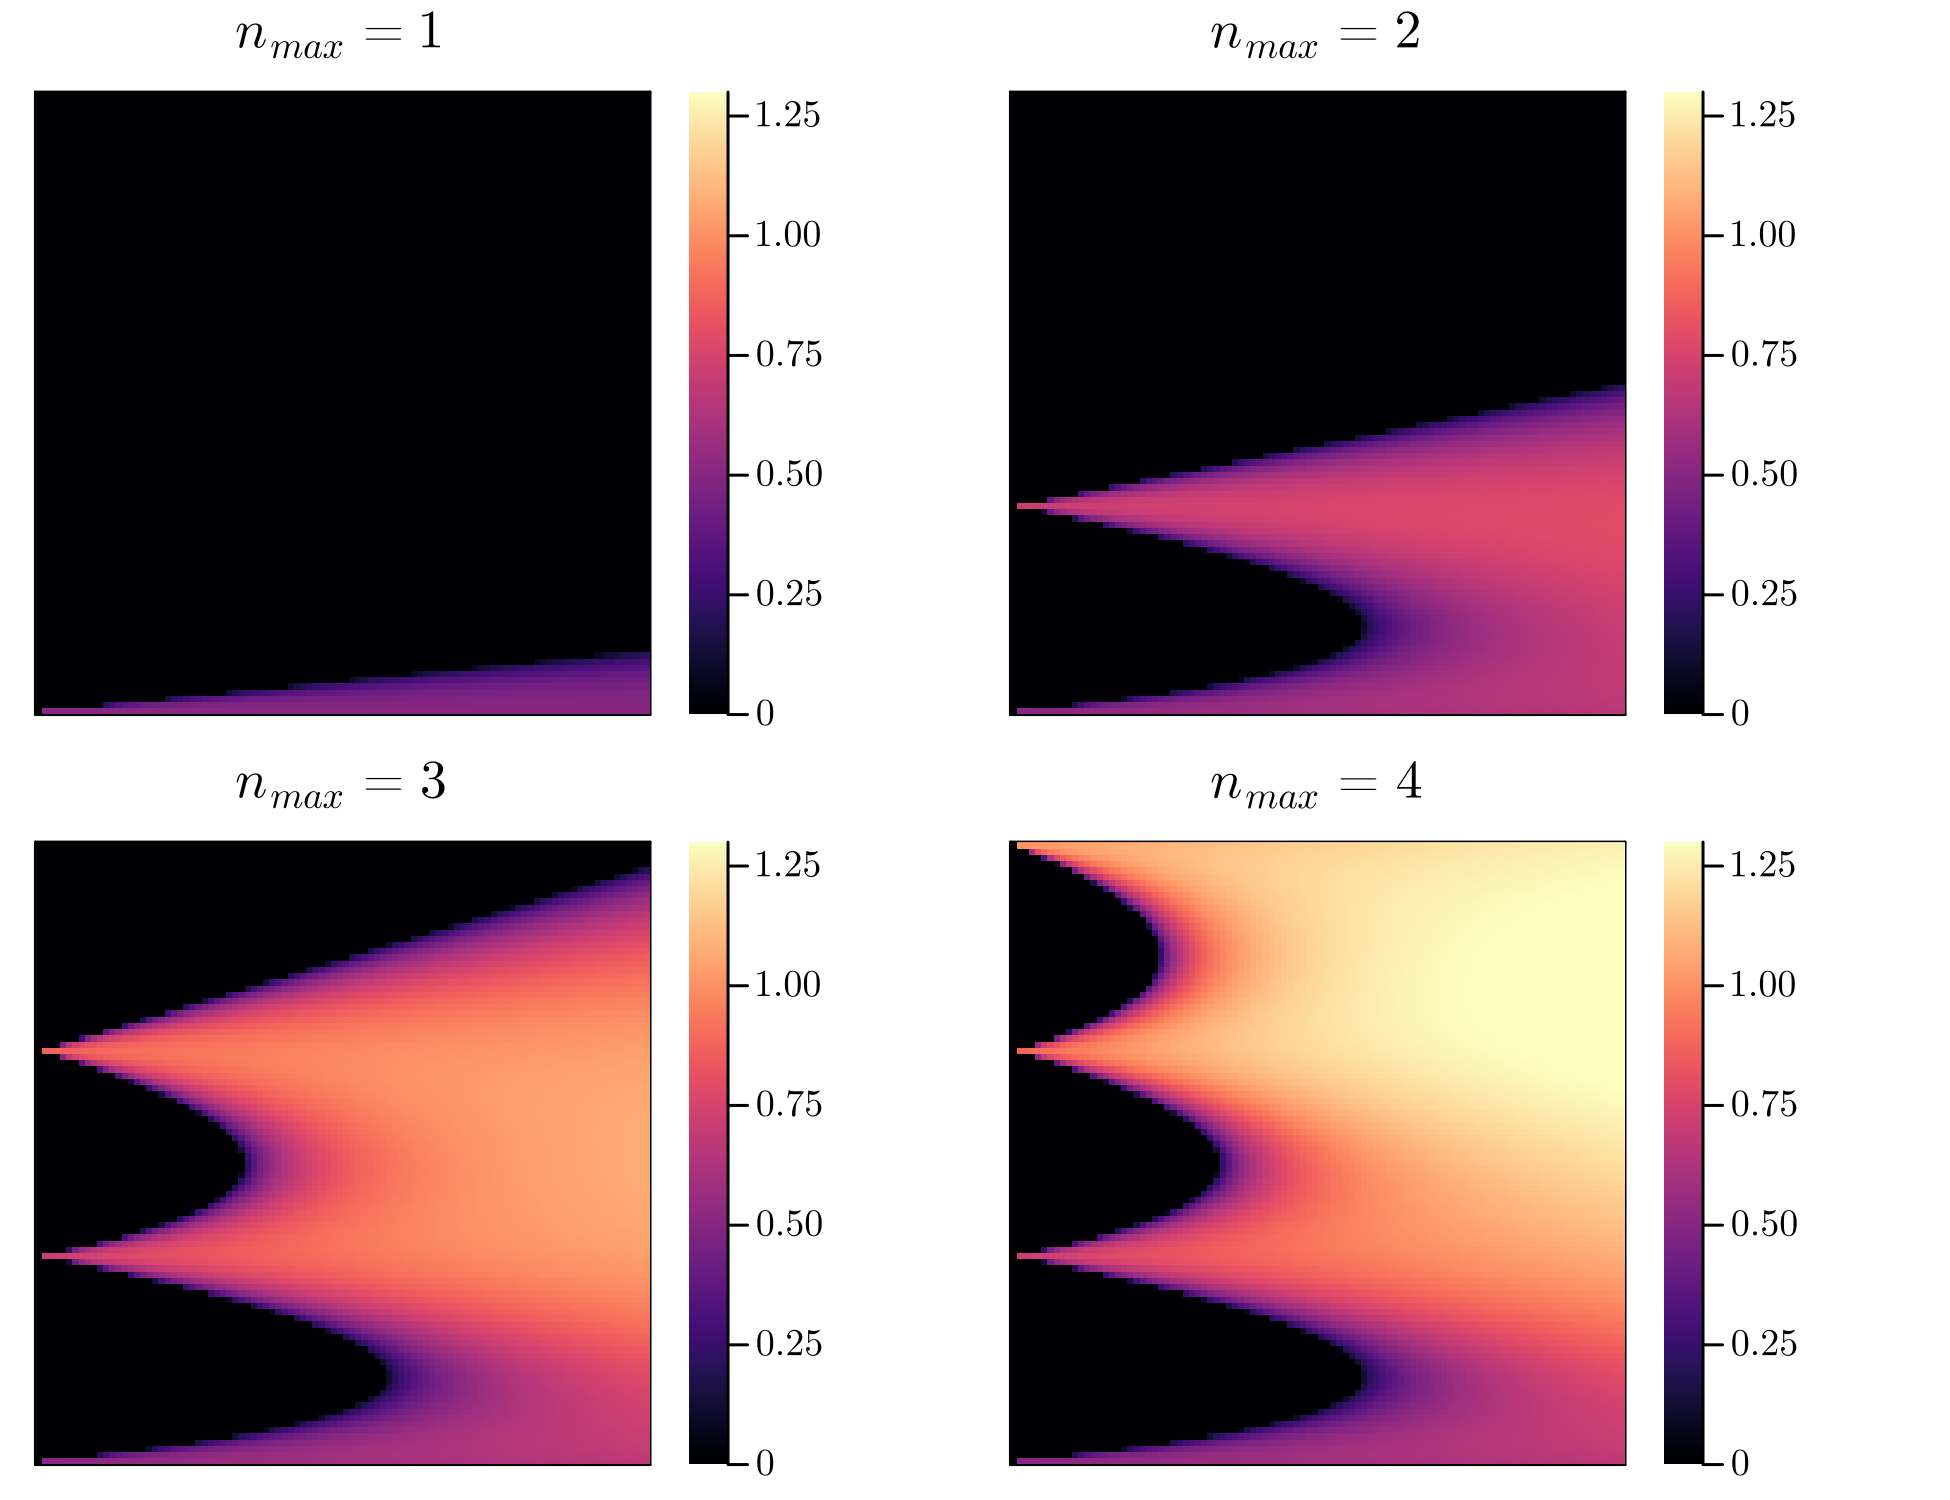
\includegraphics[width=\textwidth]{ch4/cutoff.png}
    \end{subfigure}
    \caption{Qualitative variation of phase diagram as the occupation cutoff is increased.}
    \label{fig:nmax}
\end{figure}
%%% FIG %%%
\FloatBarrier \!\!\!\!\!\!\!\!\!\!\!

Most notably, there will only be $n_{max}$ Mott lobes and for larger chemical potential, the entire parameter space will remain a Mott insulator since the maximum number of bosons is capped. However, we can see that this is a minor issue upon realizing that the physics of the low-energy lobes remain largely unaffected by the truncation and discrepancies only arise closer to the high-energy lobes. This is demonstrated in Fig. \ref{fig:nmax} and can be checked rigorously by quantifying the convergence of the phase boundaries as $n_{max}$ is increased.
\vspace{0.5cm}\\
In this thesis, we mostly focus on the first three Mott lobes, and the corresponding phase boundaries are found to converge quickly as $n_{max}$ is increased upto a value of 10.

\subsection{Extending to finite temperature}
In this section, we demonstrate that the mean-field approach is capable of handling finite temperature calculations as well. The only change required is to compute the expectation values as thermal expectations, by working with density matrices instead of the ground state. The self-consistency relation $\Psi = \langle \hat{a} \rangle_T = \Tr{\hat{a}\rho}/\Tr{\rho}$ can be recovered as well by imposing minimization of the free energy. 
%%% FIG %%%
\begin{figure}[!htb]
    \centering
    \begin{subfigure}[b]{\textwidth}  %keep total sum <1 to show in same line
        \centering
        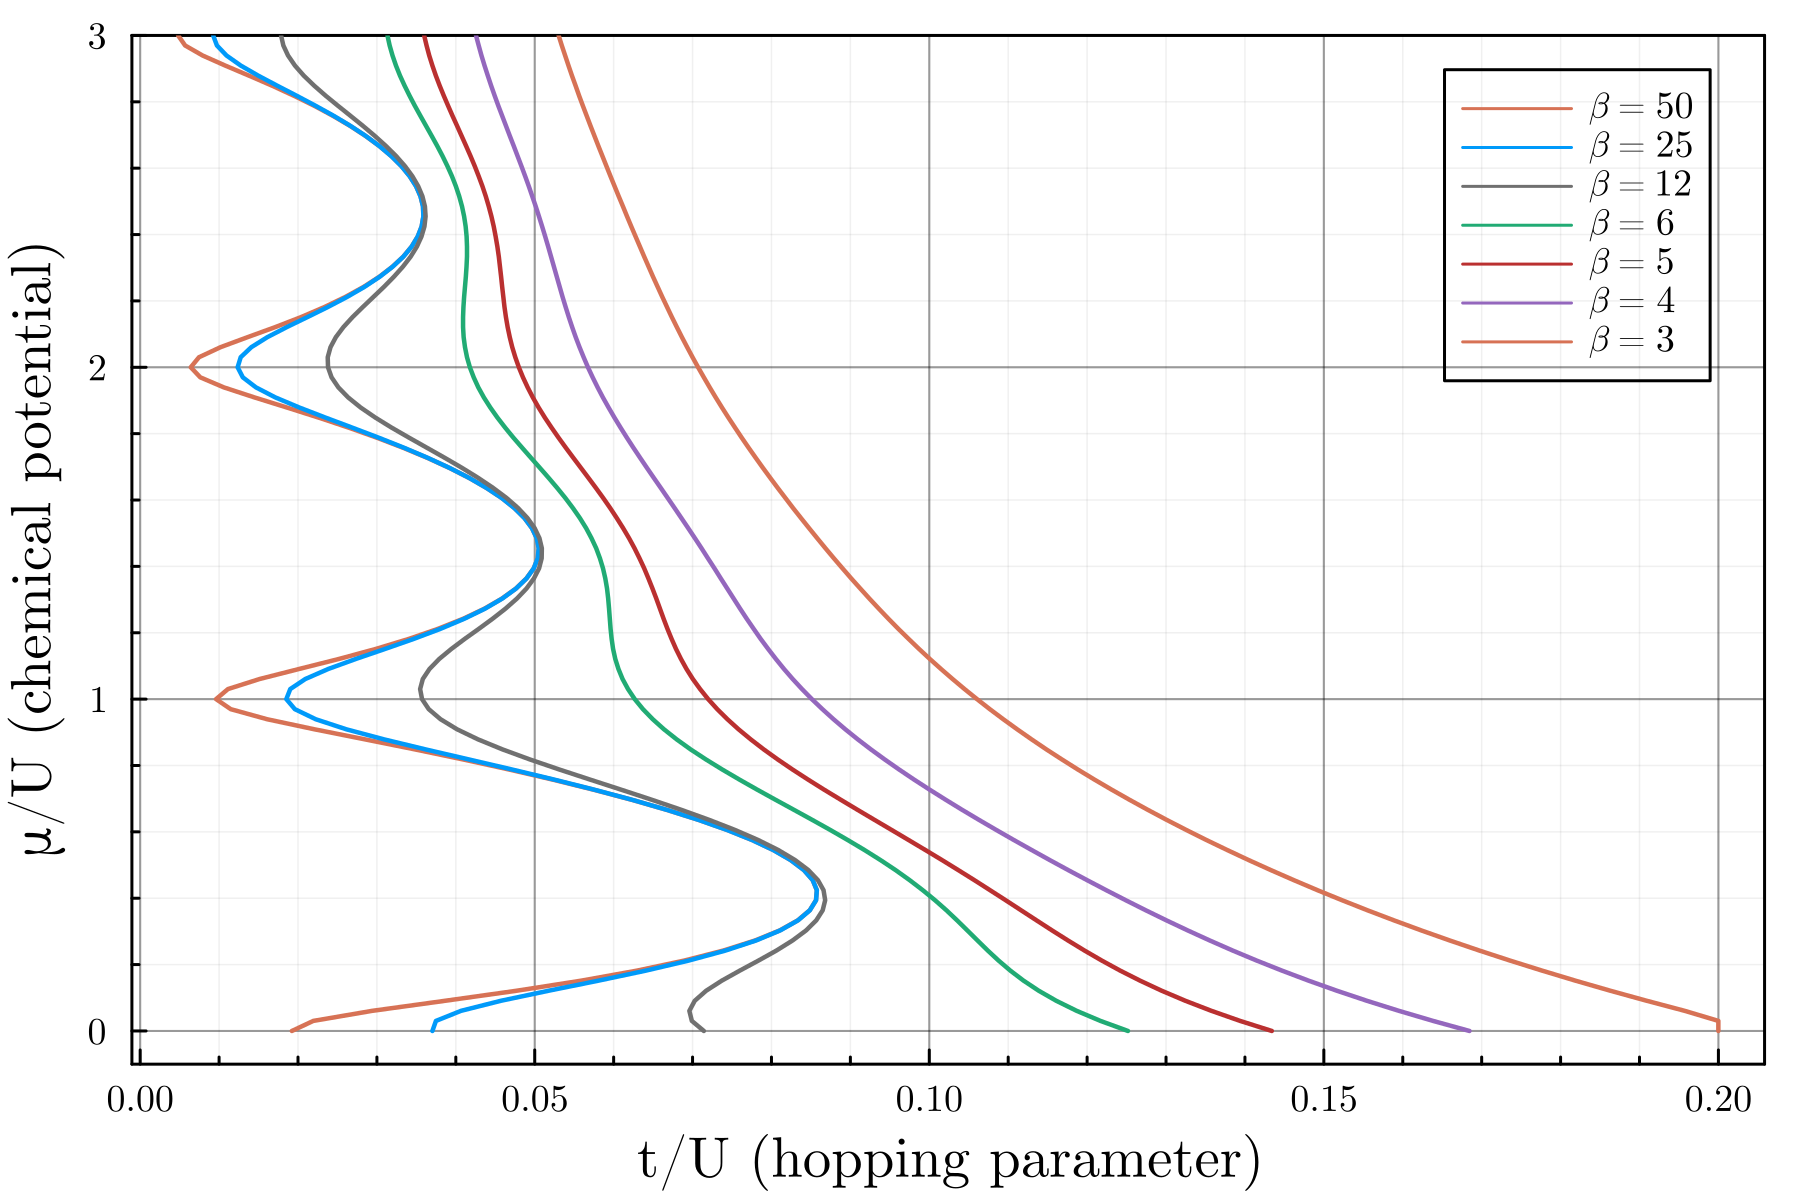
\includegraphics[width=\textwidth]{ch4/finite_temp.png}
    \end{subfigure}
    \caption{1D Mean-field phase boundaries at finite temperatures.}
    \label{fig:mft_temp}
\end{figure}
%%% FIG %%%
\FloatBarrier \!\!\!\!\!\!\!\!\!\!\!

At a finite temperature, Fig. \ref{fig:mft_temp} seemingly shows that the Mott insulator lobes coalesce into a single region as the temperature is increased. However, this is infact due to the formation of a thermally disordered phase, namely, the normal fluid. At the mean field level, it seems similar to the superfluid since it has finite compressibility and variance of occupation number. However, such a phase does not does not break the $U(1)$ symmetry and its formation is not driven by quantum fluctuations. 
\vspace{0.5cm}\\
As the temperature is increased, the Mott insulator lobes start vanishing and the extent of the superfluid region decreases as the normal fluid becomes the most stable phase throughout the parameter space. 

\subsection{An alternative de-coupling}
Decoupling the hopping term ($a_i^{\dagger}a_j$) seems ubiquitous in literature when trying to simplify the Bose-Hubbard model. Strangely, the standard scheme for the mean-field study of the (fermionic) Hubbard model involves decoupling the interaction term instead. Nothing stops us apriori from utilizing a similar scheme as well. 
\begin{align}
    &\hspace{1.2cm}\hat{n}_i = \rho_i + \delta \hat{n}_i \nonumber\\
    &\implies \delta n_i^2 = (n_i - \rho_i)(n_i - \rho_i) \approx 0 \nonumber\\
    &\implies n_i^2 \approx 2\rho_i n_i - \rho_i^2
\end{align}
The Hamiltonian can then be written as:
\begin{equation}
    H_{MF} = -t\sum_{\langle i, j \rangle} a_i^{\dagger} a_j + \sum_i \left( \mu - \frac{U}{2} + U\rho_i\right) n_i - \frac{U}{2}\sum_i \rho_i^2
\end{equation}
If we utilize translational symmetry to set $\rho_i = \rho$ and switch to the Bloch basis, we get:
\begin{equation}
    H_{MF} = -t\sum_{k} \left(\epsilon_k + \mu - \frac{U}{2} + U\rho\right) \tilde{a}_k^{\dagger} \tilde{a}_k - \frac{U}{2}M\rho^2
\end{equation}
Since this is already diagonal, the ground state would simply be a condensate in the $k$-mode with lowest energy. Note that such a decoupling still preserves the conservation of particle number and as a result, $\langle a \rangle$ can no longer serve as an order parameter for the superfluid phase. Regardless, we see that a Mott insulator can never be admitted as a ground state by such a Hamiltonian since it is always a condensate. This exercise brings to light an apparent subjectivity involved in choosing an appropriate decoupling. However, although the choice may be guided by considering the limiting behaviour of the system, the right choice is the one that generates the lowest ground state energy. Such a claim can be made rigorous if we view the mean field treatment as a variational method\cite{sachdev_2011}.

\subsection{Pitfalls}
Although the mean-field approach has allowed us to gain some insight on the BHM, it is only reliable for qualitative results. Particularly, since we have ignored higher order quantum fluctuations, we tend to over-estimate the extent of the ordered phase. Further, most of the information about the lattice geometry and dimensionality is lost as we only take into account the co-ordination number of each lattice site. Such a treatment only becomes exact in the limit of an infinite-dimensional lattice geometry. We will now proceed to formulate a numerical technique that tackles these issues.

\section{Cluster Mean Field Theory}
This technique can be seen a middle ground between exact diagonalization and single-site mean field theory as portrayed in Fig. \ref{fig:cmft_diagram}.
%%% FIG %%%
\begin{figure}[!htb]
    \centering
    \begin{subfigure}[b]{\textwidth}  %keep total sum <1 to show in same line
        \centering
        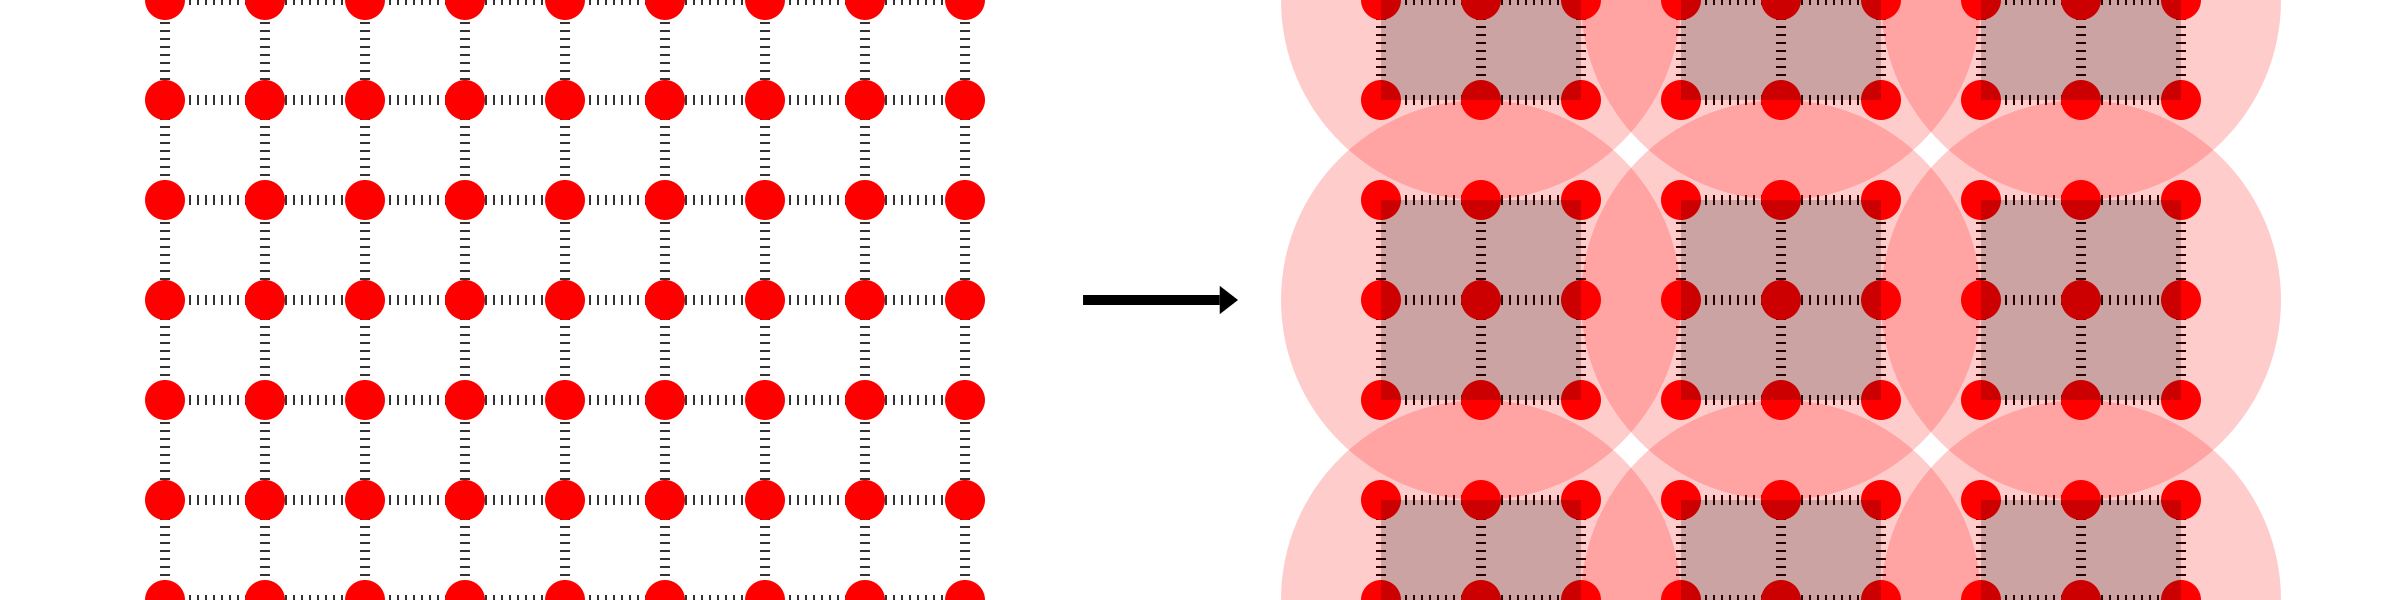
\includegraphics[width=\textwidth]{ch4/CMFTdiagram.png}
    \end{subfigure}
    \caption{Pictorial representation of CMFT in 2D}
    \label{fig:cmft_diagram}
\end{figure}
%%% FIG %%%
\FloatBarrier \!\!\!\!\!\!\!\!\!\!\!

 We demonstrate the idea by considering a 1D lattice with $M$ sites. The chain can then be divided into $N_c$ clusters, each of length $L$ such that $M = LN_c$. The hopping term of the BHM can now be written as follows.
 \begin{equation}
    H_{hop} = -t\sum_{j=0}^{N_c - 1}\sum_{l = 1}^{L-1} (a_{Lj+l}^{\dagger}a_{Lj+l+1} + a_{Lj+l + 1}^{\dagger}a_{Lj+l}) - t\sum_{j=0}^{N_c-1}(a_{Lj+L}^{\dagger}a_{Lj+L+1} + a_{Lj+L+1}^{\dagger}a_{Lj+L})
 \end{equation}
where the first term, $H_{\text{intra}}$ couples the sites within each cluster, and the second term, $H_{\text{inter}}$ couples the different clusters. The main idea of CMFT is to treat the intra-cluster coupling exactly and the inter-cluster coupling at a mean-field level. Following the same de-coupling we used in Eq. \eqref{eq:decoupling_scheme}, we obtain:
\begin{equation}
    H_{\text{intra}} = -t \sum_{j=0}^{N-1}[(a_{Lj+L}^{\dagger} + a_{Lj+L+1}^{\dagger})\Psi + (a_{Lj+L} + a_{Lj+L+1})\Psi^*] + 2tN_c|\Psi|^2
\end{equation}
where $\Psi = \langle a_i \rangle$ is the mean-field order parameter. Putting all this together, we arrive at the cluster-decoupled Hamiltonian.
\begin{equation}
    H_{MF}\{\Psi\} = \sum_{j=0}^{N_c-1} H_{MF}^L\{\Psi\} = \sum_{j=0}^{N_c-1} (H_j^L + V_j^L\{\Psi\})
\end{equation}
\begin{equation}
    H_j^L = -t\sum_{l=1}^{L-1}(a_{Lj + l}^{\dagger}a_{Lj + l+1} + a_{Lj + l+1}^{\dagger}a_{Lj + l}) + \frac{U}{2}\sum_{l=1}^L n_{Lj + l}(n_{Lj + l} - 1) - \mu \sum_{l=1}^L n_{Lj + l}
\end{equation}
\begin{equation}
    V^L_j\{\Psi\} = -t(\Psi(a_{Lj + 1}^{\dagger} + a_{Lj + L}^{\dagger}) + \Psi^*(a_{Lj + 1} + a_{Lj + L})) + 2t|\Psi|^2    
\end{equation}
Again, without loss of generality one can assume $\Psi \in \mathbb{R}$ and solve the system in a self-consistent manner. This procedure mostly remains the same for higher dimensions\cite{McIntosh_2012} and other lattice geometries\cite{Malakar_2020, Malakar_2023} but requires more book-keeping as we are forced to include more mean-field parameters (one for each distinct kind of boundary site in the cluster). 
\newpage
\subsection{Results}

%%% FIG %%%
\begin{figure}[!htb]
    \centering
    \begin{subfigure}[b]{0.6\textwidth}  %keep total sum <1 to show in same line
        \centering
        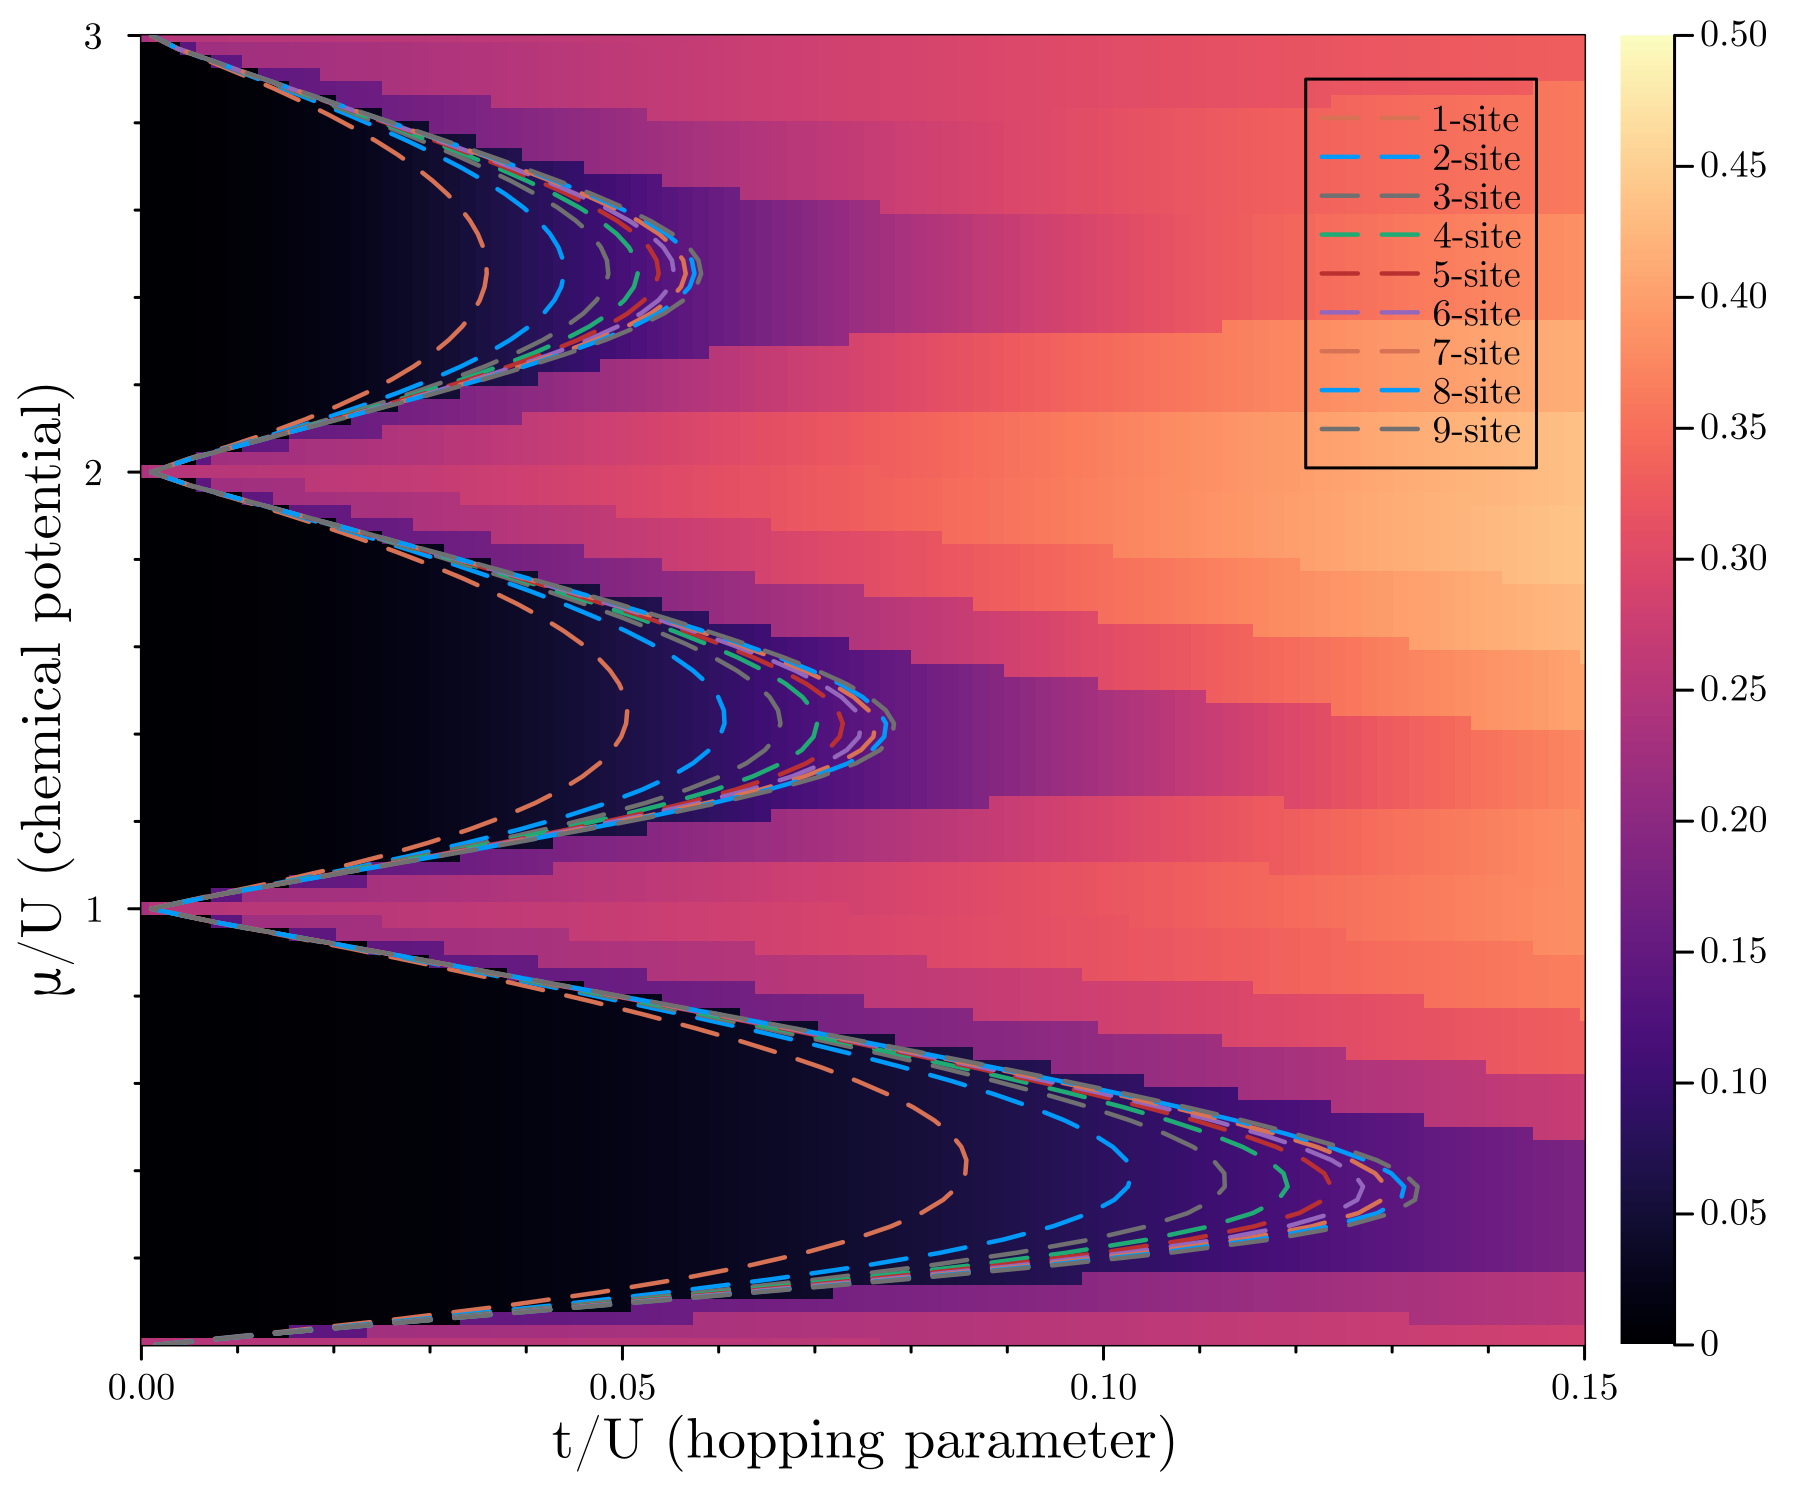
\includegraphics[width=\textwidth]{ch4/phase_diagram_cmft.png}
        \caption{Phase boundary}
    \end{subfigure}
    \hspace{1em}  %\hfill
    \begin{subfigure}[b]{0.3\textwidth}
        \centering
        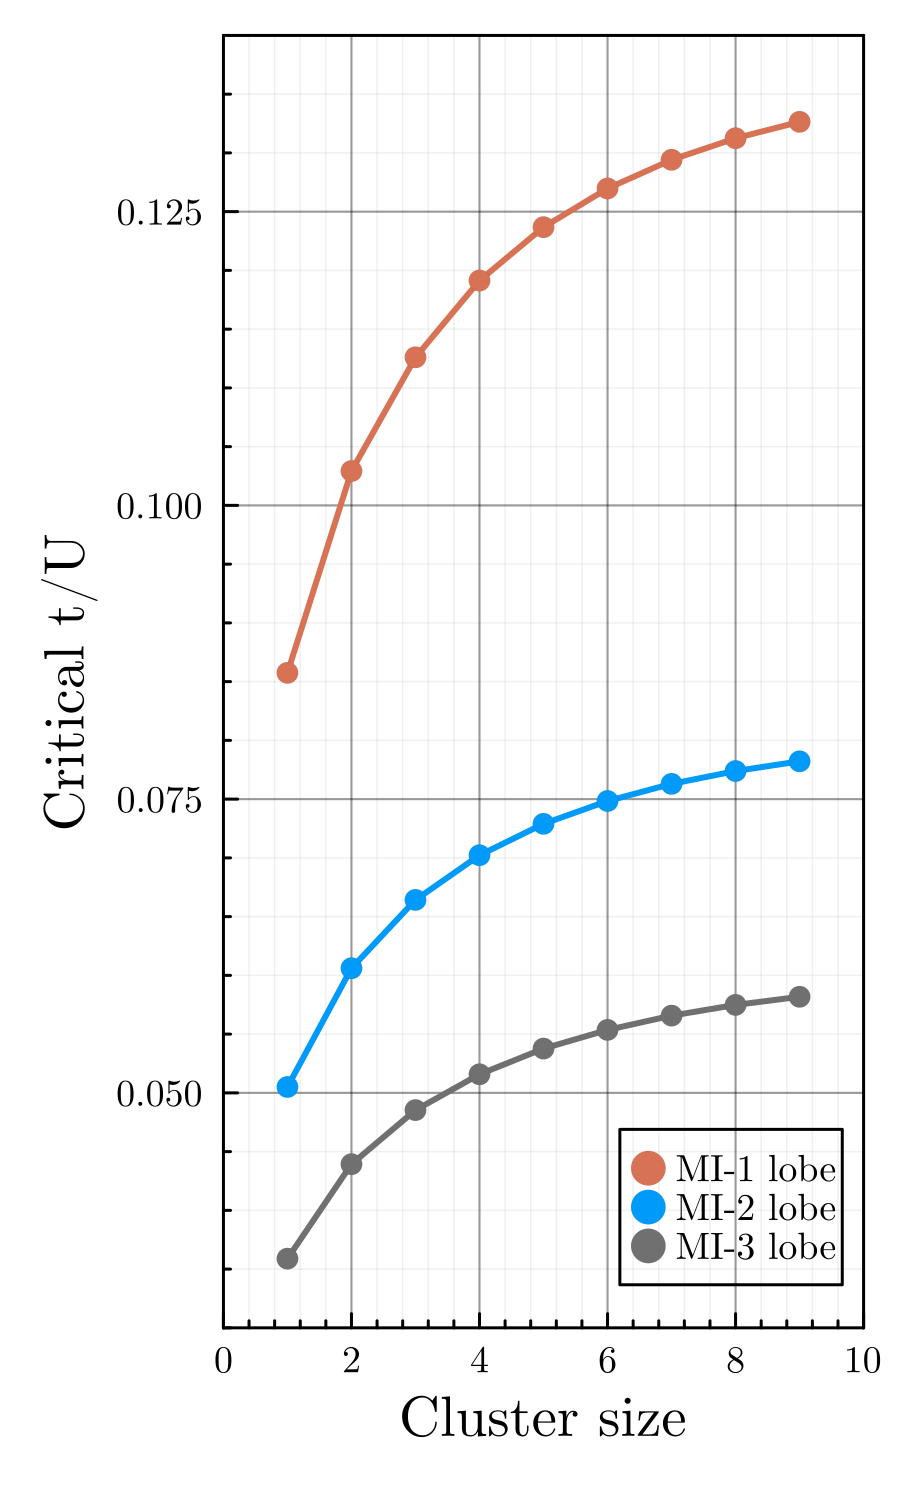
\includegraphics[width=\textwidth]{ch4/cmft_crit.png}
        \caption{Critical point of Mott lobes}
    \end{subfigure}
    \caption{Comparison of 1D CMFT results for various cluster sizes. The heatmap indicates the variance of occupation number obtained through exact diagonalization of the system with $M=6$ and $N_{max}=4$.}
    \label{}
\end{figure}
%%% FIG %%%
\FloatBarrier \!\!\!\!\!\!\!\!\!\!\!

We see that the estimation of the phase boundaries improves as we increase the size of the cluster. However, while the computational cost still grows exponentially, the marginal improvement of the boundary estimate diminishes for larger cluster sizes. Although this might only be the case for 1D systems, we decide not to employ this technique for further analysis due to the complexity involved in an implementation for arbitrary lattice geometries. 

\chapter{Dipolar bosons in a lattice}\label{ch4}
In this chapter, we consider spinless bosons that have a permanent dipole moment and are trapped in an optical lattice. Since dipole-dipole interactions fall off as $V(r) \sim 1/r^3$, the contact interaction alone results in a poor description of the system. To remedy this, we take into account the nearest neighbour interactions as well.
\begin{equation}
    H = -t\sum_{\langle i, j\rangle} a_i^{\dagger}a_j + \frac{U}{2}\sum_i n_i(n_i - 1) + \frac{V}{2}\sum_{\langle i, j \rangle} n_i n_j - \mu \sum_i n_i
\end{equation}
Such a Hamiltonian is generally called the Extended Bose-Hubbard model (eBHM)\cite{Baier16}. The analysis that follows will apply for any microscopic interactions that are long-range in nature to justify considering the nearest neighbour interactions, and not just those that have a dipolar origin. The details only become relevant if we wish to compute experimentally achievable values of $V$\cite{Zhang_2021} (as in Sec. \ref{sec:calc_params}). However, we will not be dealing with this in the thesis.
\vspace{0.5cm}\\
We are specifically interested in the case when $U, V > 0$. In such a situation, the on-site and nearest neighbour interactions compete with each other, introducing the possibility of breaking the translational symmetry. We proceed now to study how this affects the ground-state phases through a mean-field analysis. 

\section{Mean Field Theory}
The mean-field decoupling of the eBHM largely proceeds the same way as with the BHM. The key difference is that we also need to decouple the $n_in_j$ term by introducing another set of mean-field parameters, $\{\rho_i\}$. 

\begin{minipage}{0.5\linewidth}
    \begin{align}
        &\hspace{1.2cm}\hat{a}_i = \Psi_i + \delta \hat{a}_i \nonumber\\
        &\implies \delta a_i^{\dagger} \delta a_j = (a_i^{\dagger} - \Psi_i^*)(a_j - \Psi_j) \approx 0 \nonumber\\
        &\implies a_i^{\dagger}a_j \approx \Psi_ja_i^{\dagger} + \Psi_i^*a_j - \Psi_i^*\Psi_j \nonumber
    \end{align}
\end{minipage}%
\begin{minipage}{0.5\linewidth}
    \begin{align}
        &\hspace{1.2cm}\hat{n}_i = \rho_i + \delta \hat{n}_i \nonumber\\
        &\implies \delta n_i \delta n_j = (n_i - \rho_i)(n_j - \rho_j) \approx 0 \nonumber\\
        &\implies n_i n_j \approx \rho_j n_i + \rho_i n_j - \rho_i\rho_j
    \end{align}
\end{minipage}
\vspace{0.5cm}\\
Note here that since $n_i = a_i^{\dagger}a_i$, we could have simply used the first decoupling for the $n_i n_j$ term as well. However, the resulting mean-field Hamiltonian turns out to be incapable of hosting the phases we are interested in. In any case, neglecting the terms of $\mathcal{O}(\delta a_i^2)$ is a lower order approximation than neglecting $\mathcal{O}(\delta n_i^2)$.
\vspace{0.5cm}\\
Proceeding with the derivation, we already know the decoupling for the hopping term from Eq. \eqref{eq:mft_hop}. The decoupling for the interaction term proceeds in a similar way. 
\begin{align}
    H_{int}/(V/2) &= \sum_{\langle i, j\rangle} n_i n_j \nonumber\\
    &= \sum_{\langle i, j\rangle} (\rho_jn_i + \rho_in_j - \rho_i\rho_j) \nonumber\\
    &= \sum_i \big (\sum_{j \in N_i} \rho_j\big ) n_i + \sum_i \big (\sum_{j \in N_i} \rho_j\big ) n_i - \sum_i \big (\sum_{j \in N_i} \rho_j\big) \rho_i
\end{align}

Defining the mean order parameter, $\overline{\rho}_i = \frac{1}{z}\sum_{j \in N_i} \rho_j$, we obtain the interaction term at the mean-field level.
\begin{align}
    H_{int}/(zV/2) = \sum_i (2\overline{\rho}_i n_i - \overline{\rho}_i\rho_i)
\end{align}
We can then write the entire site-decoupled Hamiltonian which depends on a set of $2M$
mean-field parameters, $\{\Psi_i, \rho_i\}$.
\begin{equation}
    H_i\{\Psi_i, \rho_i\} = -zt (\overline{\Psi}_i a_i^{\dagger} + \overline{\Psi}_i^* a_i - \overline{\Psi}_i\Psi_i^*) + \frac{zV}{2} (2\overline{\rho}_i n_i - \overline{\rho}_i\rho_i) + \frac{U}{2}n_i(n_i - 1) - \mu n_i
\end{equation}

Following the derivation in Sec. \ref{sec:bhm_mft}, we might now be tempted to set $\Psi_i = \Psi \text{ and } \rho_i = \rho$. However, this is a bad choice to make for the eBHM, because as mentioned earlier, the interplay of the interaction terms allows the possibility of breaking the translational symmetry. Making this assumption would incorrectly ignore the existence of certain phases and misrepresent the extents of others. Instead, we can consider arbitrary periodic patterns across the lattice and write the mean-field Hamiltonian for a single unit-cell\cite{Gheeraert2011} as follows.
\begin{align}\label{eq:ebhm_mft}
    H_{MF, UC} = &\sum_{X \in UC} \left [-zt(\overline{\Psi}_X a_X^{\dagger} + \overline{\Psi}_X^* a_X) + (zV\overline{\rho}_X - \mu)n_X + \frac{U}{2}n_X(n_X - 1)\right ] \nonumber\\
    - &\sum_{X \in UC} \left [zt\overline{\Psi}_i\Psi_i^* -  \frac{zV}{2} \overline{\rho}_X\rho_X \right ]
\end{align}


\section{Results}

\subsection{1D lattice}
Since the interaction term only acts between nearest neighbour pairs, there is only one periodic pattern that is possible for the 1D lattice. This simply comprises of a unit cell with two sites $A$ and $B$ that repeat through the lattice. It is prudent now to introduce the notion of a connectivity matrix that uniquely specifies the unit cell.

\begin{minipage}{0.4\linewidth}
    \begin{equation*}
        M_{UC} =  \bordermatrix{ & A & B \cr
        A & 0 & 2 \cr
        B & 2 & 0 }
    \end{equation*}
\end{minipage}%
\begin{minipage}{0.5\linewidth}
%%% FIG %%%
\centering
\vspace{0.2cm}
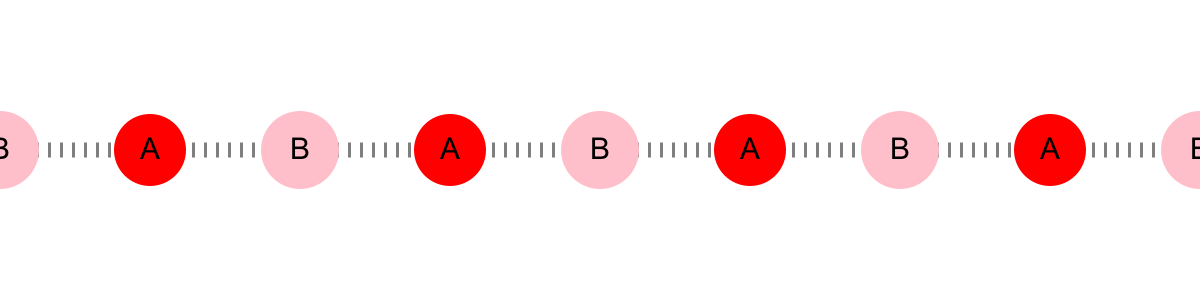
\includegraphics[width = 0.8\textwidth]{ch5/1d_sublattice.png}
%%% FIG %%%
\end{minipage}
\vspace{0.5cm}\\
Such a matrix is always symmetric and is equivalent to representing the lattice as an undirected graph. Although this is not strictly required for the 1D chain, we will find it useful to distinguish different patterns in more complicated lattice geometries. The connectivity matrix also gives us a succinct way to compute the mean-field parameters.
\begin{equation}\label{eq:unit_cell}
    \begin{pmatrix}
        \overline{\Psi}_A \\
        \overline{\Psi}_B
    \end{pmatrix} = M_{UC}  \begin{pmatrix}
        \Psi_A \\
        \Psi_B
    \end{pmatrix}
\end{equation}
which in this case simply gives us $\overline{\Psi}_A = 2\Psi_B$ and $\overline{\Psi}_B = 2\Psi_A$. The same relation also holds for $\overline{\rho}_X$ and $\rho_X$. We can now construct the Hamiltonian and self-consistently diagonalize it to obtain the ground state solution.

\subsubsection{\large Classifying the phases}
Note that we now have four mean-field parameters, $\{\Psi_A, \Psi_B, \rho_A, \rho_B\}$ and the various phases can be classified using them as follows.
\begin{itemize}
    \item When $\rho_A = \rho_B = \rho$ and $\Psi_A = \Psi_B = \Psi$, this effectively restores translational invariance and describes a Mott Insulator when $\Psi = 0$ and a Superfluid otherwise.
\end{itemize}
%%% FIG %%%
\begin{figure}[!htb]
    \centering
    \begin{subfigure}[b]{0.45\textwidth}  %keep total sum <1 to show in same line
        \centering
        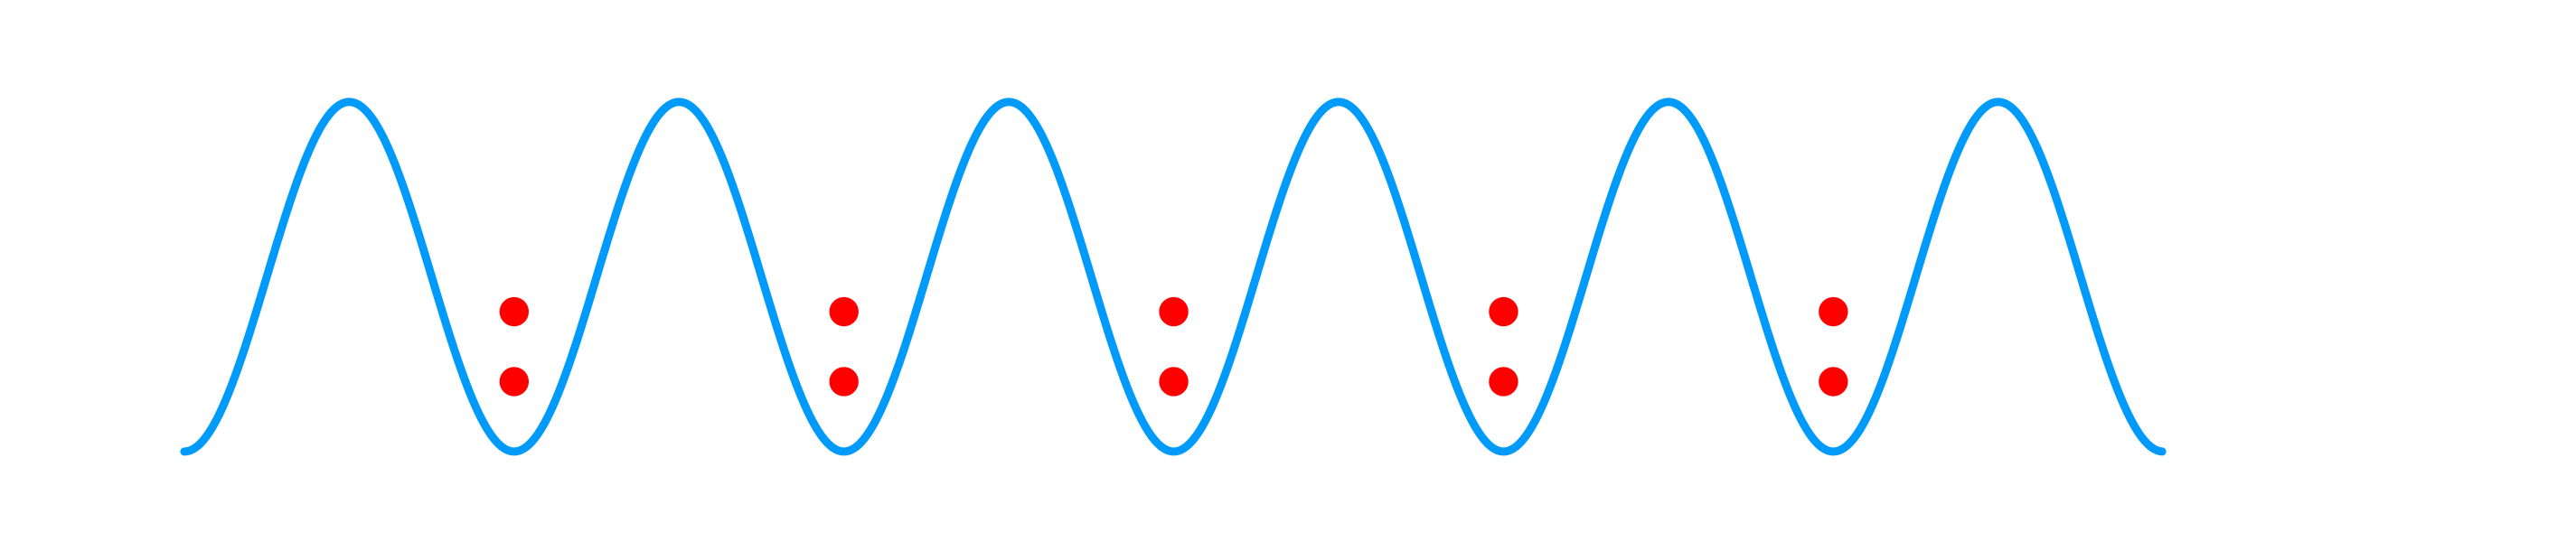
\includegraphics[width=\textwidth]{ch5/MIdiagram.png}
        \caption{Mott insulator}
    \end{subfigure}
    \hspace{1em}  %\hfill
    \begin{subfigure}[b]{0.45\textwidth}
        \centering
        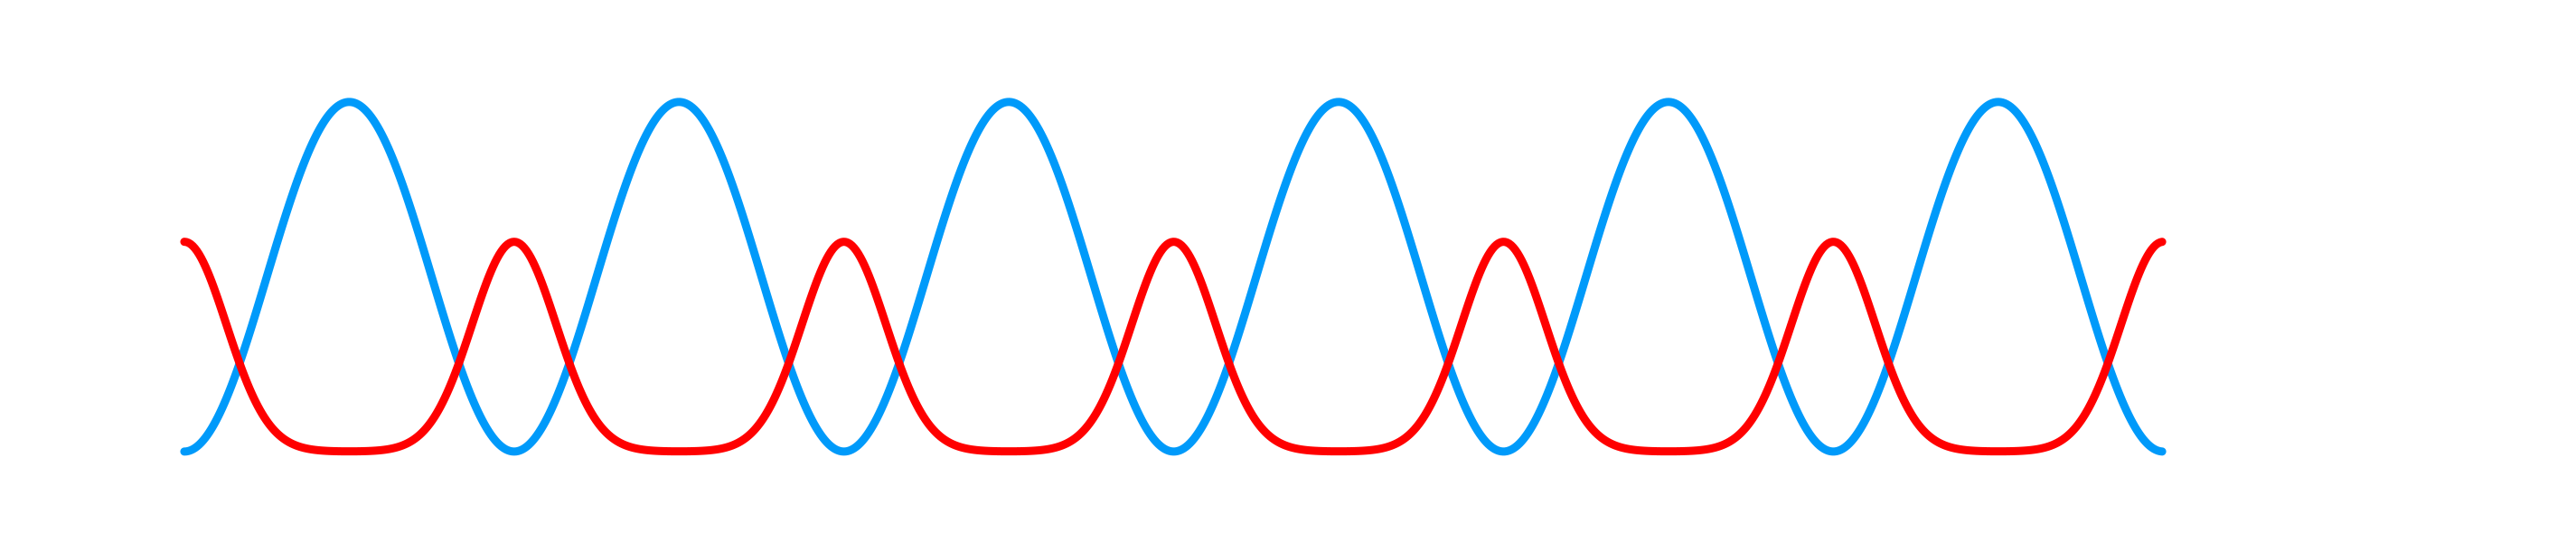
\includegraphics[width=\textwidth]{ch5/SFdiagram.png}
        \caption{Super-fluid}
    \end{subfigure}
    \caption{Pictorial representation of the BHM phases}
    \label{}
\end{figure}
%%% FIG %%%
\FloatBarrier \!\!\!\!\!\!\!\!\!\!\!
\vspace{-0.3cm}
\begin{itemize}
    \item When $\rho_A \neq \rho_B$, this indicates a modulation of the average density of particles over the lattice and describes a Density Wave when $\Psi_A = \Psi_B = 0$ and a Supersolid otherwise.
\end{itemize}

%%% FIG %%%
\begin{figure}[!htb]
    \centering
    \begin{subfigure}[b]{0.45\textwidth}  %keep total sum <1 to show in same line
        \centering
        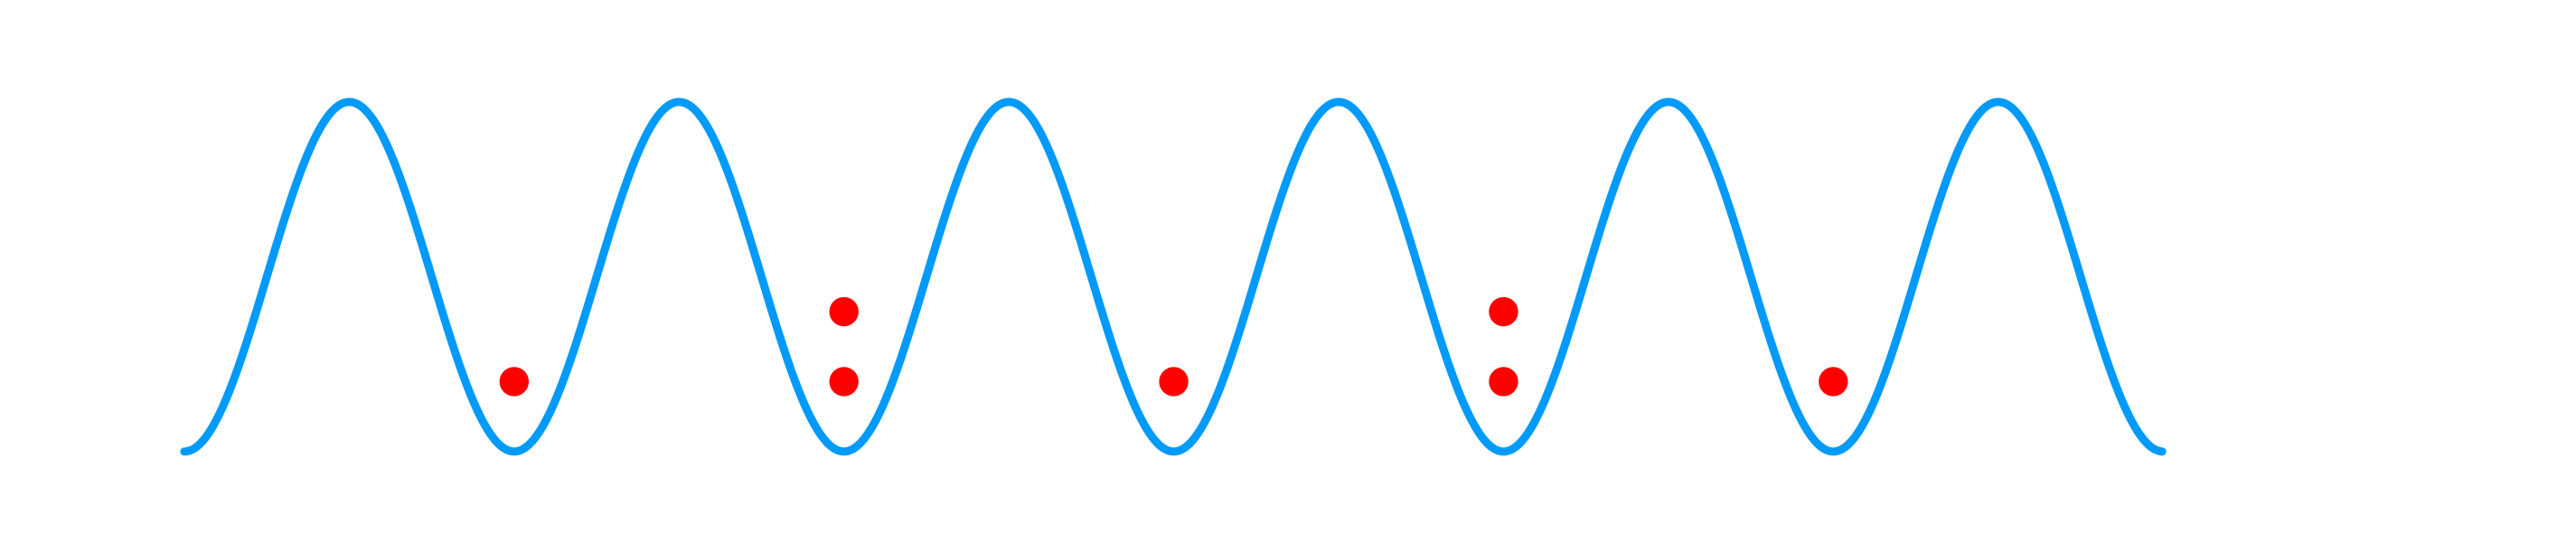
\includegraphics[width=\textwidth]{ch5/DWdiagram.png}
        \caption{Density Wave}
    \end{subfigure}
    \hspace{1em}  %\hfill
    \begin{subfigure}[b]{0.45\textwidth}
        \centering
        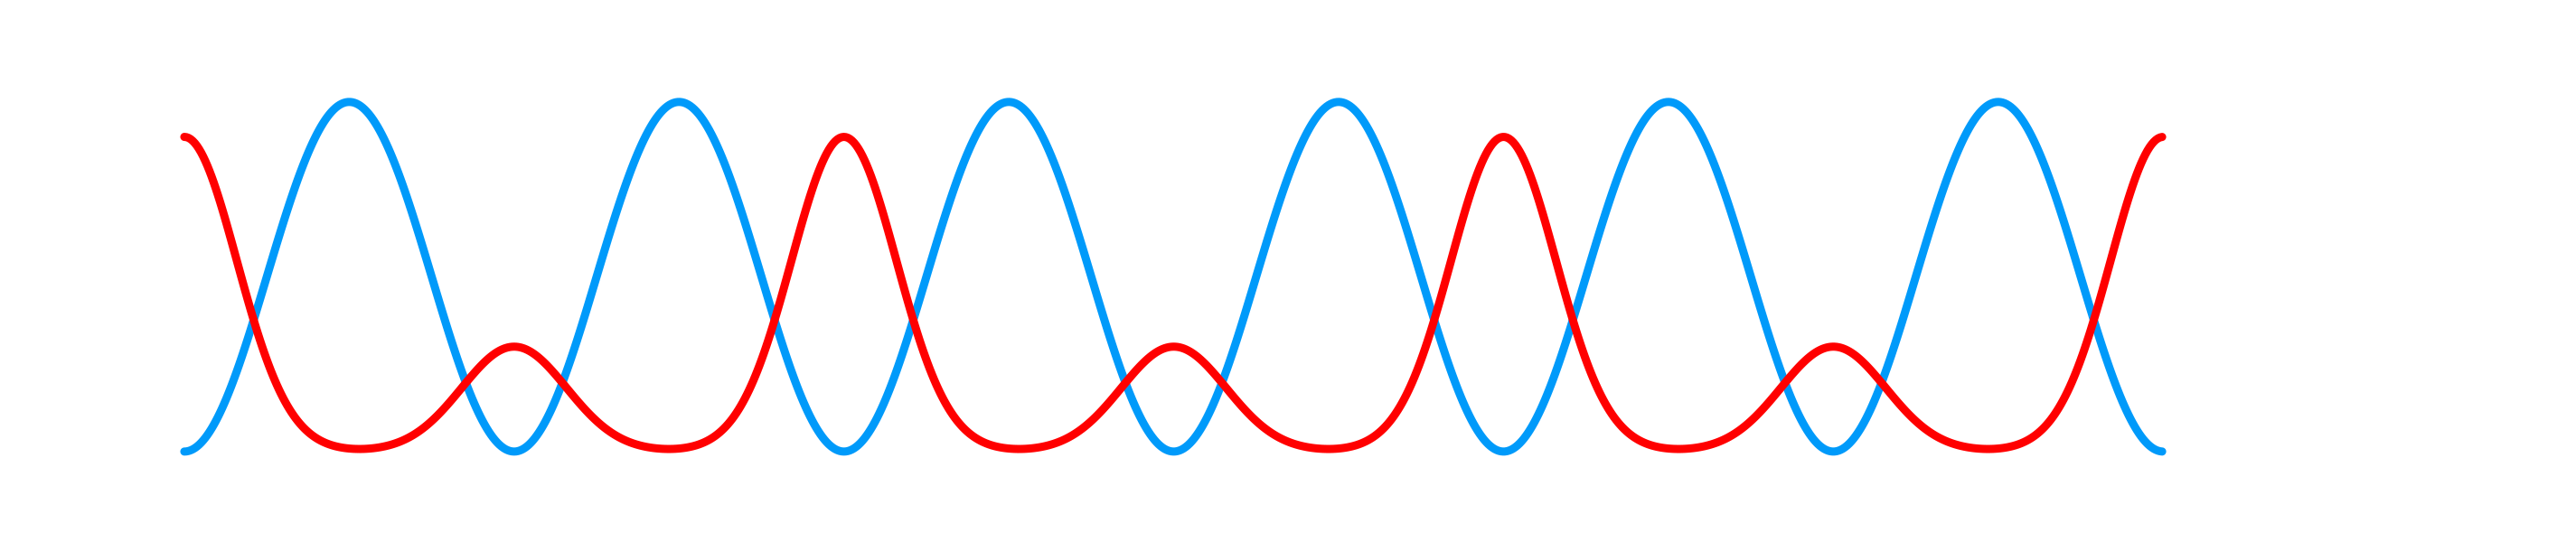
\includegraphics[width=\textwidth]{ch5/SSdiagram.png}
        \caption{Super-solid}
    \end{subfigure}
    \caption{Pictorial representation of the eBHM phases}
    \label{}
\end{figure}
%%% FIG %%%
\FloatBarrier \!\!\!\!\!\!\!\!\!\!\!

It is not surprising that the eBHM also hosts Mott insulator and superfluid phases since the BHM can be recovered in the limit $V\to 0$. When we have $zV \sim U$, however, two new analogous phases are introduced due to density modulations. The density wave phase can simply be interpreted as two inter-weaving Mott insulators with different occupation numbers. On the other hand, the supersolid can naively be described as a phase that exhibits superflow while also having some kind of crystalline order due to the periodic density modulations. Such an interpretation is rather imprecise\cite{Boninsegni_2012}, but the characterization of the phase is unambiguous atleast at the mean-field level.

%%% FIG %%%
\begin{figure}[!htb]
    \centering
    \begin{subfigure}[b]{\textwidth}  %keep total sum <1 to show in same line
        \centering
        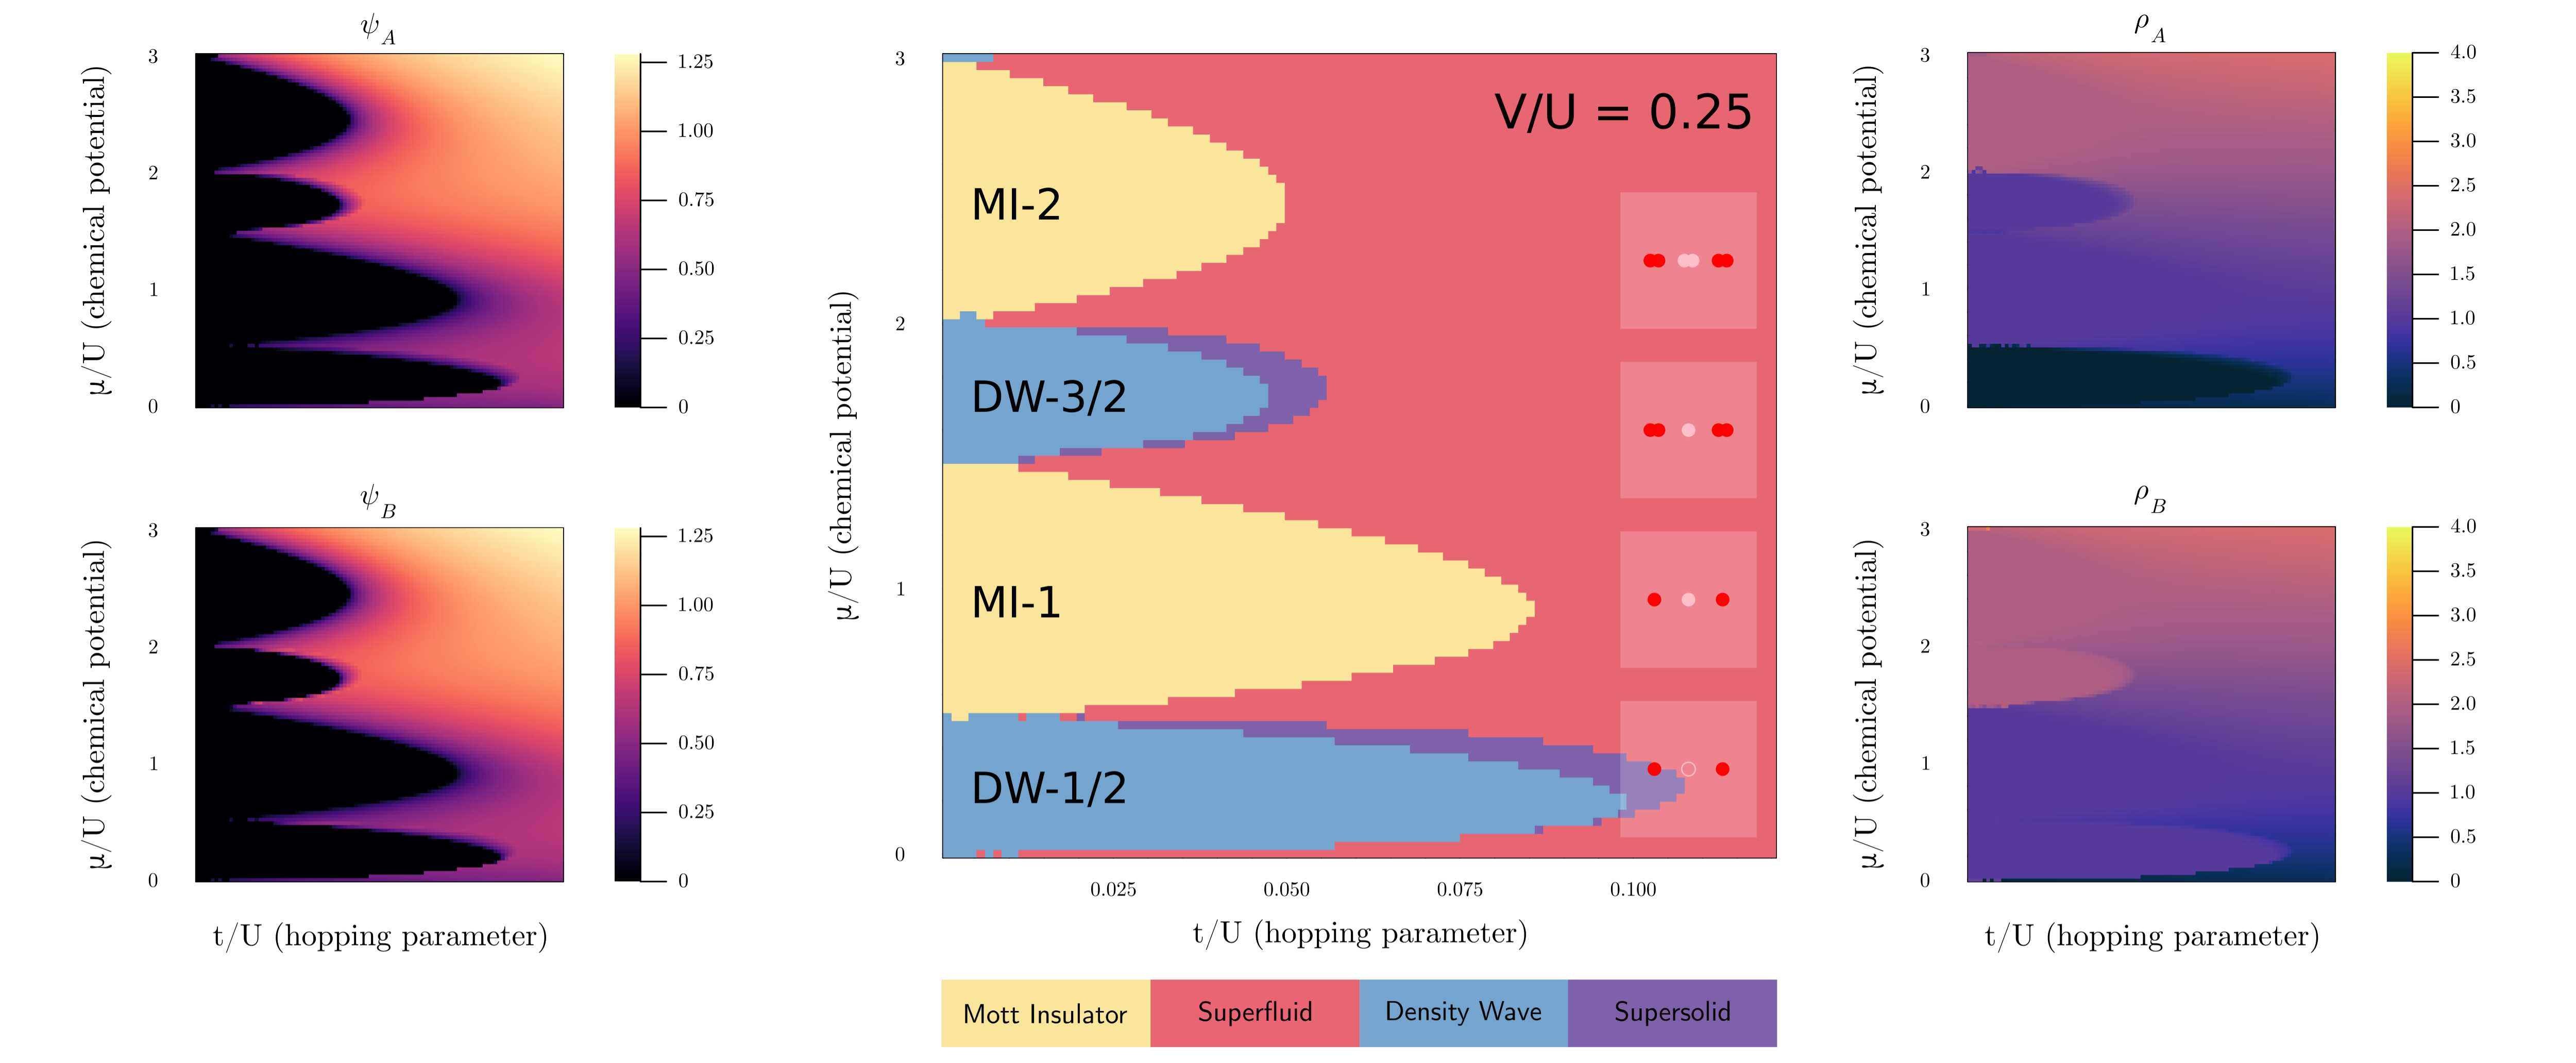
\includegraphics[width=\textwidth]{ch5/1dnew.png}
    \end{subfigure}
    \caption{Mean-field phase diagram of 1D lattice}
    \label{fig:ebhm_1d}
\end{figure}
%%% FIG %%%
\FloatBarrier \!\!\!\!\!\!\!\!\!\!\!

We can see from Fig. \ref{fig:ebhm_1d} that for an intermediate value of $V/U$, all four phases can exist in the $t-\mu$ plane. The density wave seems to appear as lobes in a similar manner to the Mott insulator. Peculiarly, the supersolid phase is only ever observed at the 'edges' of these density wave lobes. Consequently, there is no possibility of finding a phase transition directly from the density wave to the superfluid phase. Similarly, there is no direct transition from a Mott insulator to a supersolid. This seems to support the fact that a quantum phase transition can only occur if it involves breaking a single symmetry of the system.
\vspace{0.5cm}\\
We also note that we can label the density wave lobes with their average filling just as we differentiated Mott insulator lobes with their occupation number. However, this does not uniquely identify them, since a density wave having a filling of $(1, 2)$ and $(0, 3)$ will both have an average occupation of $3/2$ as seen in Fig. \ref{fig:ebhm_sq}.

\newpage
\subsection{2D square lattice}
For a square lattice, we can come up with more than one possible repeating unit cell that breaks translational symmetry. In such a case, we must find the solution in either case and only admit the one having lowest ground state energy.

\begin{minipage}{0.4\linewidth}
    \begin{equation*}
        M_{UC} =  \bordermatrix{ & A & B \cr
        A & 0 & 4 \cr
        B & 4 & 0 }
    \end{equation*}
\end{minipage}%
\hfill
\begin{minipage}{0.5\linewidth}
%%% FIG %%%
\centering
\vspace{0.2cm}
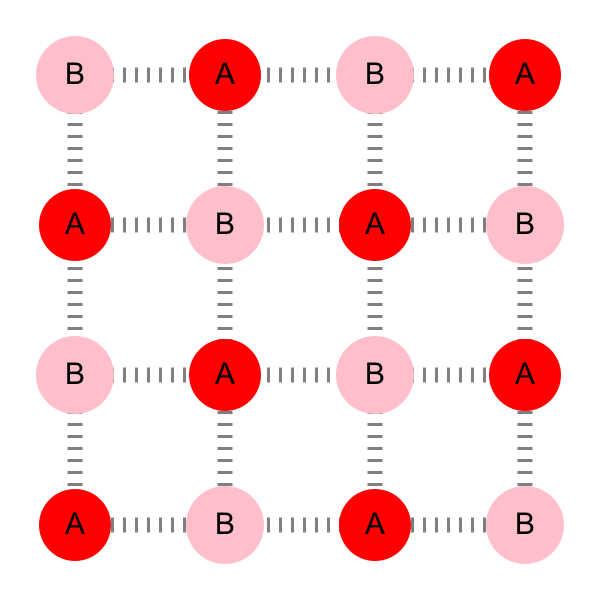
\includegraphics[width = 0.5\textwidth]{ch5/sq_sublattice1.png}
%%% FIG %%%
\end{minipage}
\vspace{0.5cm}\\
\begin{minipage}{0.4\linewidth}
    \begin{equation*}
        M_{UC} =  \bordermatrix{ & A & B \cr
        A & 2 & 2 \cr
        B & 2 & 2 }
    \end{equation*}
\end{minipage}%
\hfill
\begin{minipage}{0.5\linewidth}
%%% FIG %%%
\centering
\vspace{0.2cm}
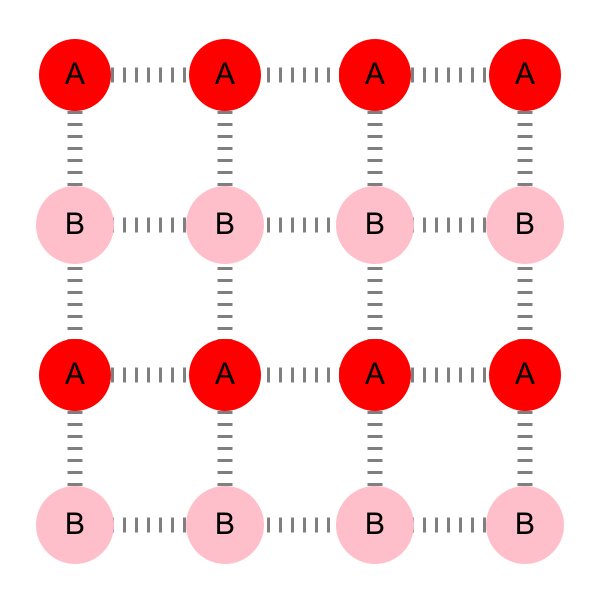
\includegraphics[width = 0.5\textwidth]{ch5/sq_sublattice2.png}
%%% FIG %%%
\end{minipage}
\vspace{0.3cm}\\
It turns out that the first pattern satisfies this condition for all parameter regimes of interest. 
\vspace{-0.4cm}
%%% FIG %%%
\begin{figure}[!htb]
    \centering
    \begin{subfigure}[b]{0.77\textwidth}  %keep total sum <1 to show in same line
        \centering
        \includegraphics[width=\textwidth]{ch5/sq_2dnew.png}
    \end{subfigure}
    \caption{Mean-field phase diagrams of 2D square lattice}
    \label{fig:ebhm_sq}
\end{figure}
%%% FIG %%%
\FloatBarrier \!\!\!\!\!\!\!\!\!\!\!

We see in Fig. \ref{fig:ebhm_sq} that the phase diagram for a 2D square lattice qualitatively looks similar to that of the 1D lattice in Fig. \ref{fig:ebhm_1d}. This is because the connectivity matrix of the dominant pattern in either case is only different by a scaling factor of two. We also see that as $V/U$ is increased, the density wave lobes arise between Mott insulator lobes and increase in extent until the latter becomes unstable throughout the $t-\mu$ plane. Also note that the density waves become the dominant phase in the diagram roughly when $zV \sim U$ as one would expect. As a result, the phase diagram is quite rich since it not only involves transitions between different phases but also between different orders (filling fractions) of density waves.

\subsection{2D triangular lattice}
We consider the following sub-lattice pattern for our analysis of the triangular lattice.

\begin{minipage}{0.4\linewidth}
    \begin{equation*}
        M_{UC} =  \bordermatrix{ & A & B & C \cr
        A & 0 & 3 & 3 \cr
        B & 3 & 0 & 3 \cr
        C & 3 & 3 & 0 }
    \end{equation*}
\end{minipage}%
\hfill
\begin{minipage}{0.5\linewidth}
%%% FIG %%%
\centering
\vspace{0.2cm}
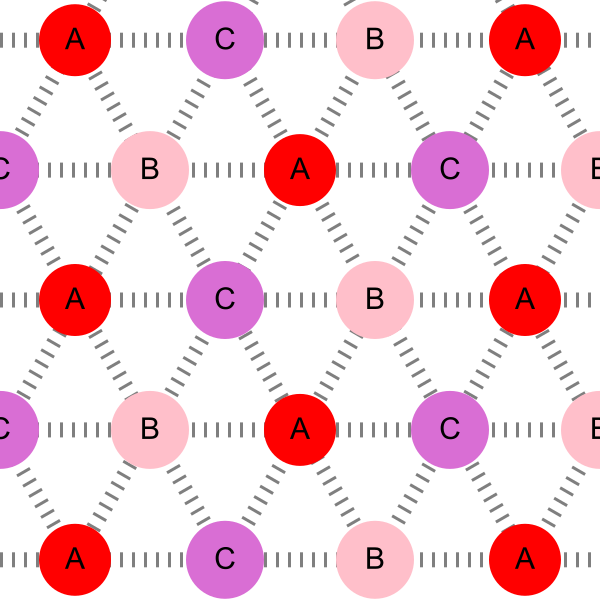
\includegraphics[width = 0.5\textwidth]{ch5/tri_sublattice1.png}
%%% FIG %%%
\end{minipage}
\vspace{0.5cm}\\

We can see in Fig. \ref{fig:ebhm_tri} that the phase diagram is quite similar to that of the square lattice except for one qualitative difference. There are now two density wave lobes between each pair of Mott insulator lobes due to possibility of additional fractional fillings in the triangular lattice (i.e, $1/3$, $2/3$, etc). 

%%% FIG %%%
\begin{figure}[!htb]
    \centering
    \begin{subfigure}[b]{0.81\textwidth}  %keep total sum <1 to show in same line
        \centering
        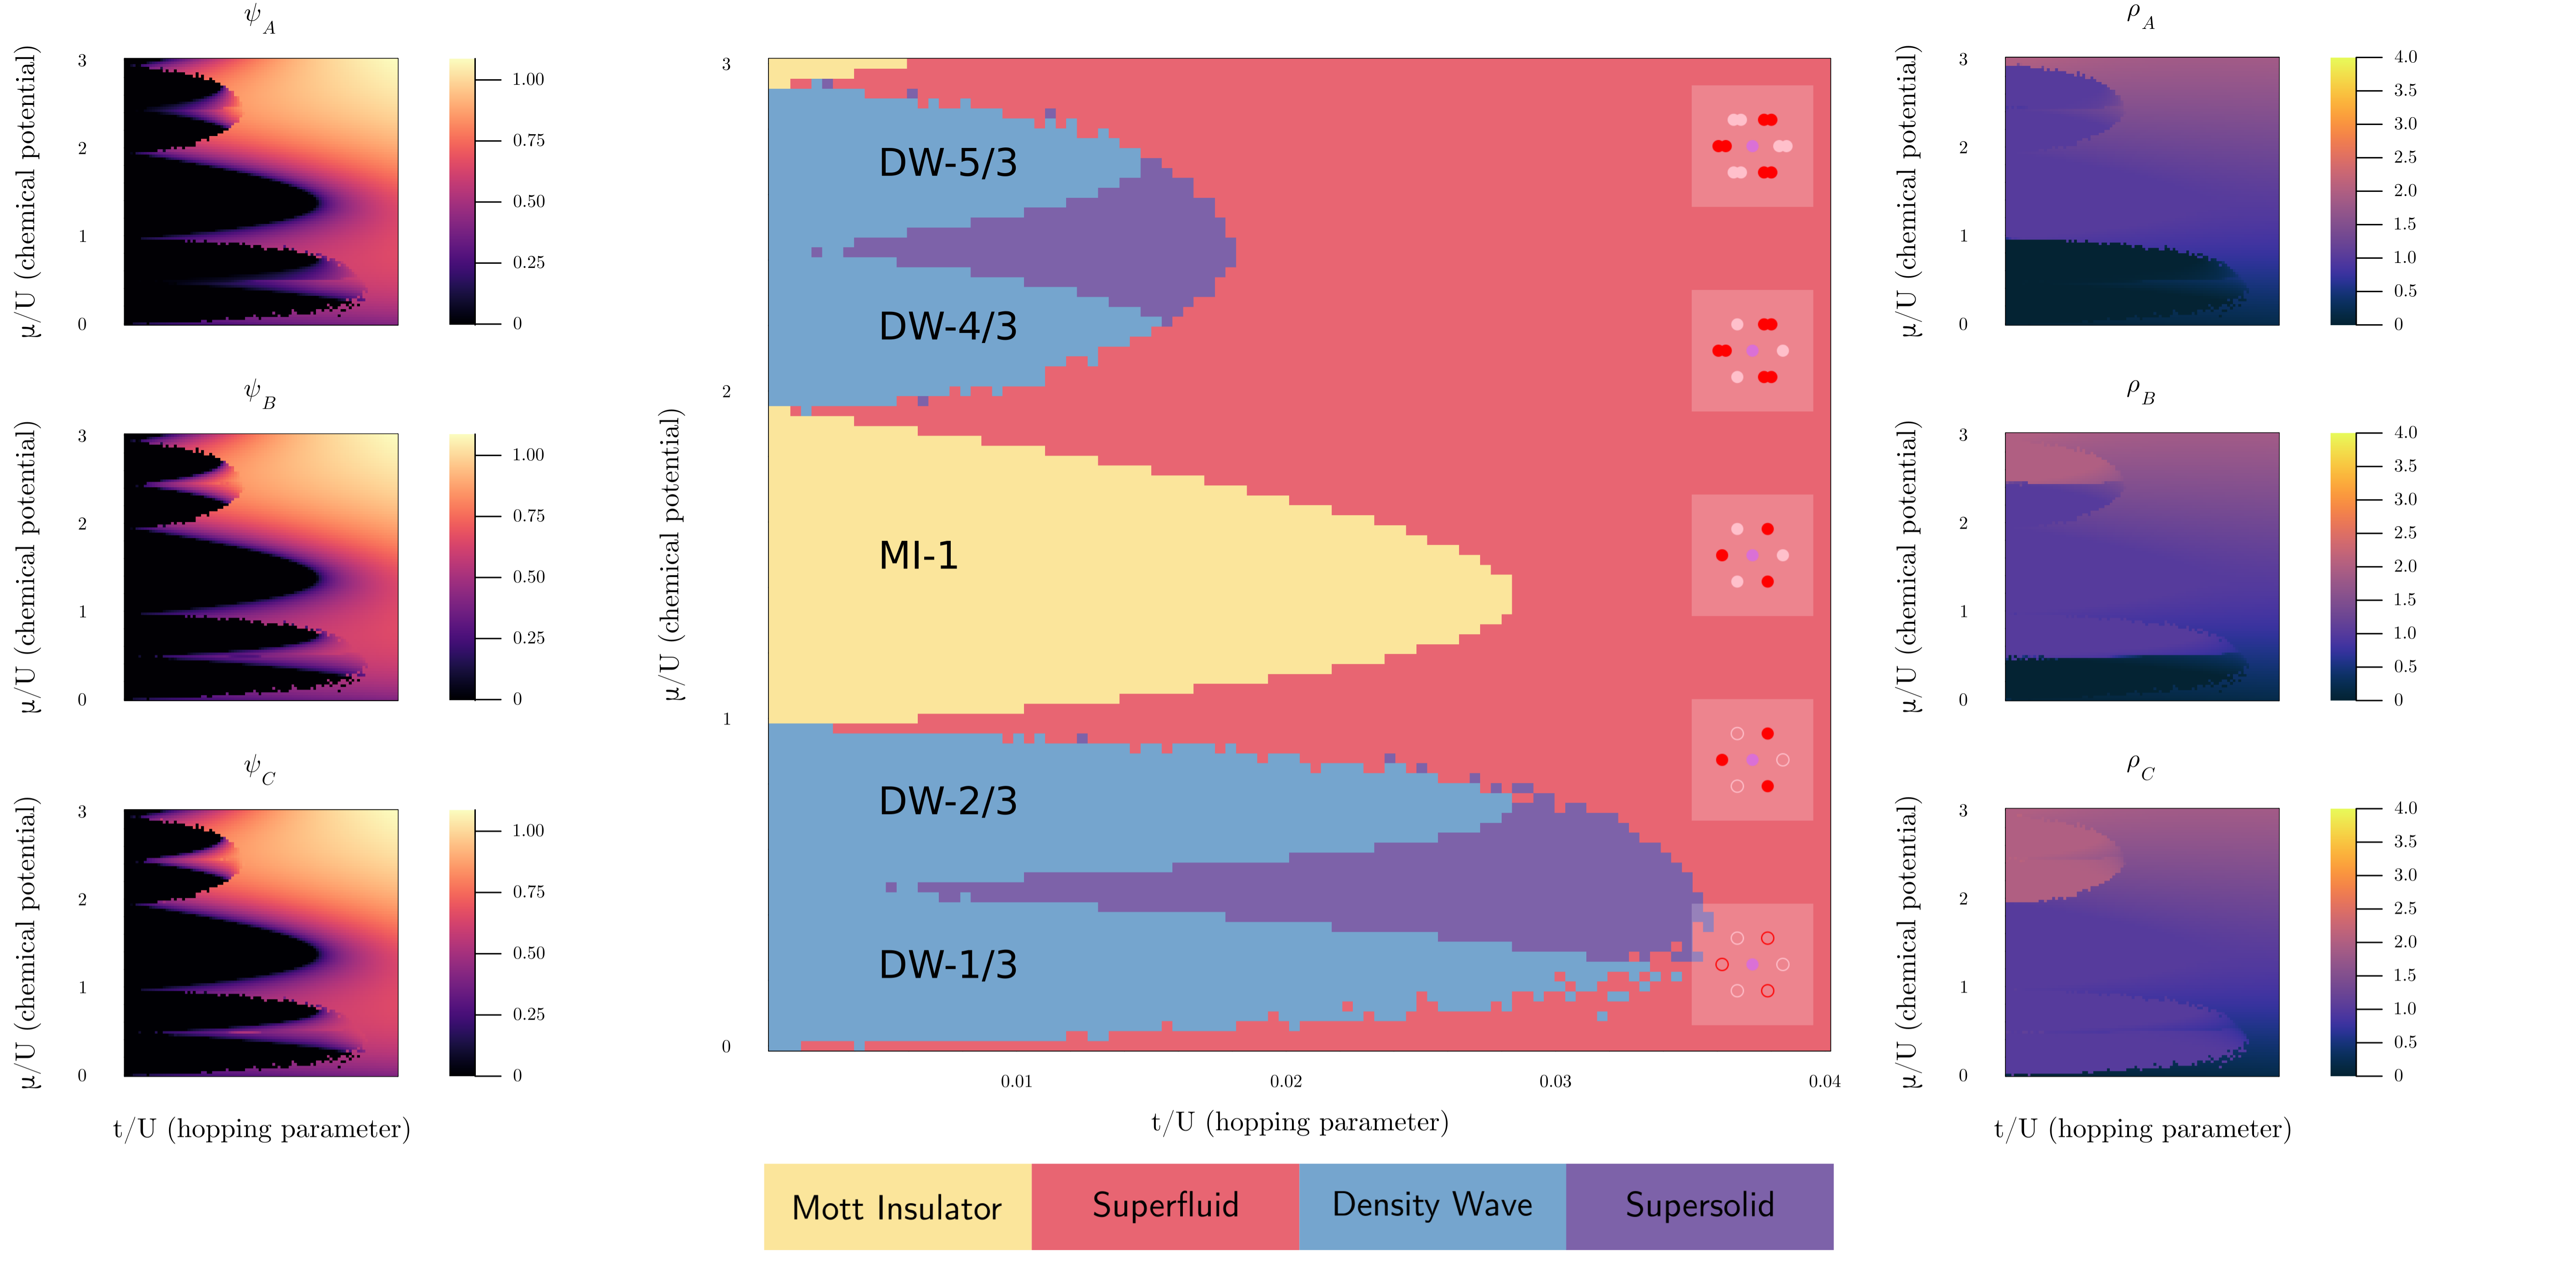
\includegraphics[width=\textwidth]{ch5/tri_2dnew.png}
    \end{subfigure}
    \caption{Mean-field phase diagram of triangular lattice (V/U = 0.34)}
    \label{fig:ebhm_tri}
\end{figure}
%%% FIG %%%
\FloatBarrier \!\!\!\!\!\!\!\!\!\!\!

\section{Issues with self-consistency}\label{sec:caveats}
When we introduced the idea of self-consistency in Chapter 4, we also described the procedure in terms of finding the fixed point of a function. This holds true for the eBHM as well, except the function is now multi-variate which significantly complicates things. For instance, our naive decision to utilize Fixed Point iteration without evaluating the conditions required for convergence has finally caught up with us. 
\vspace{0.5cm}\\
Unfortunately, the order parameters are generally related in a highly non-linear way which makes it hard to determine these conditions analytically. Instead, below are the problems that were encountered while numerically solving the system, along with possible solutions to mitigate them.

%%% FIG %%%
\begin{figure}[!htb]
    \centering
    \begin{subfigure}[b]{0.45\textwidth}  %keep total sum <1 to show in same line
        \centering
        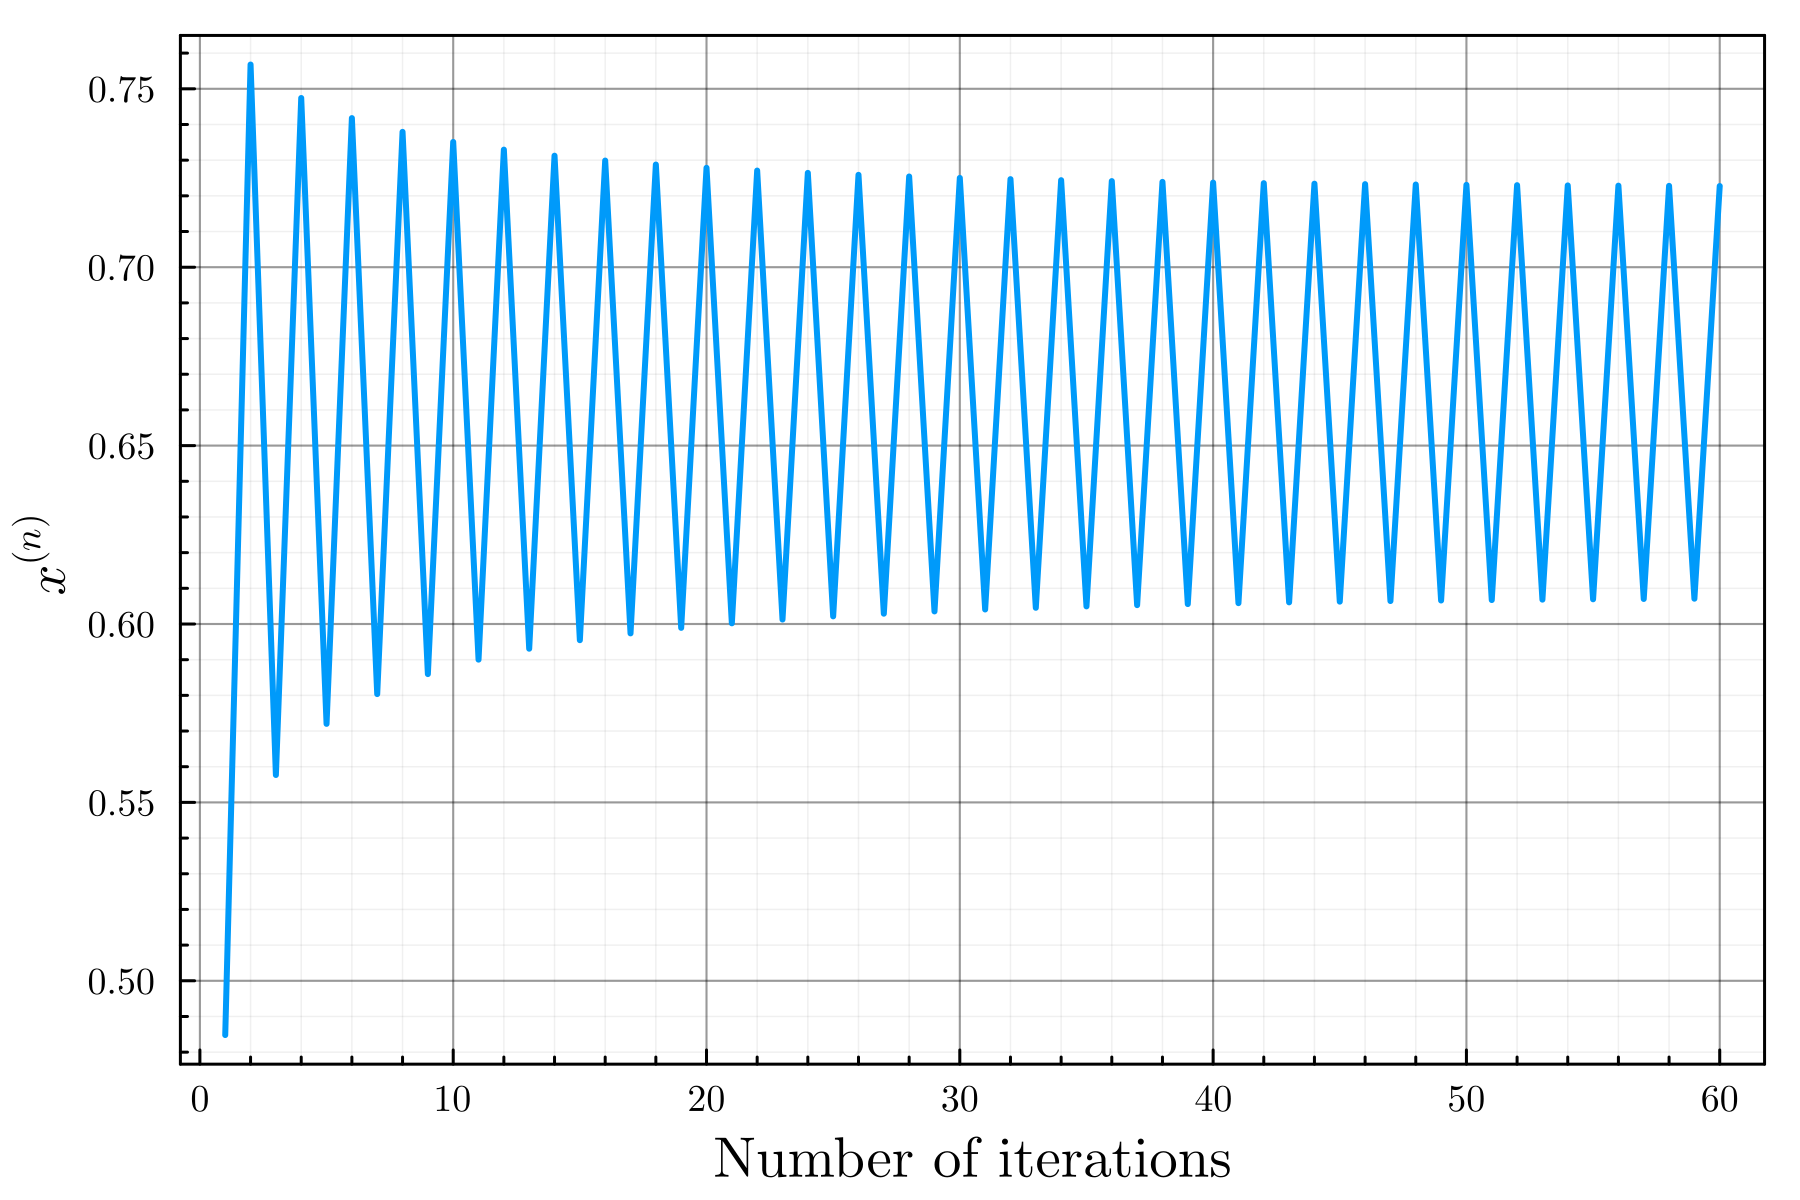
\includegraphics[width=\textwidth]{ch5/convergence_2cycle.png}
        \caption{2-cycle: $r = 3.03$}
    \end{subfigure}
    \hspace{1em}  %\hfill
    \begin{subfigure}[b]{0.45\textwidth}
        \centering
        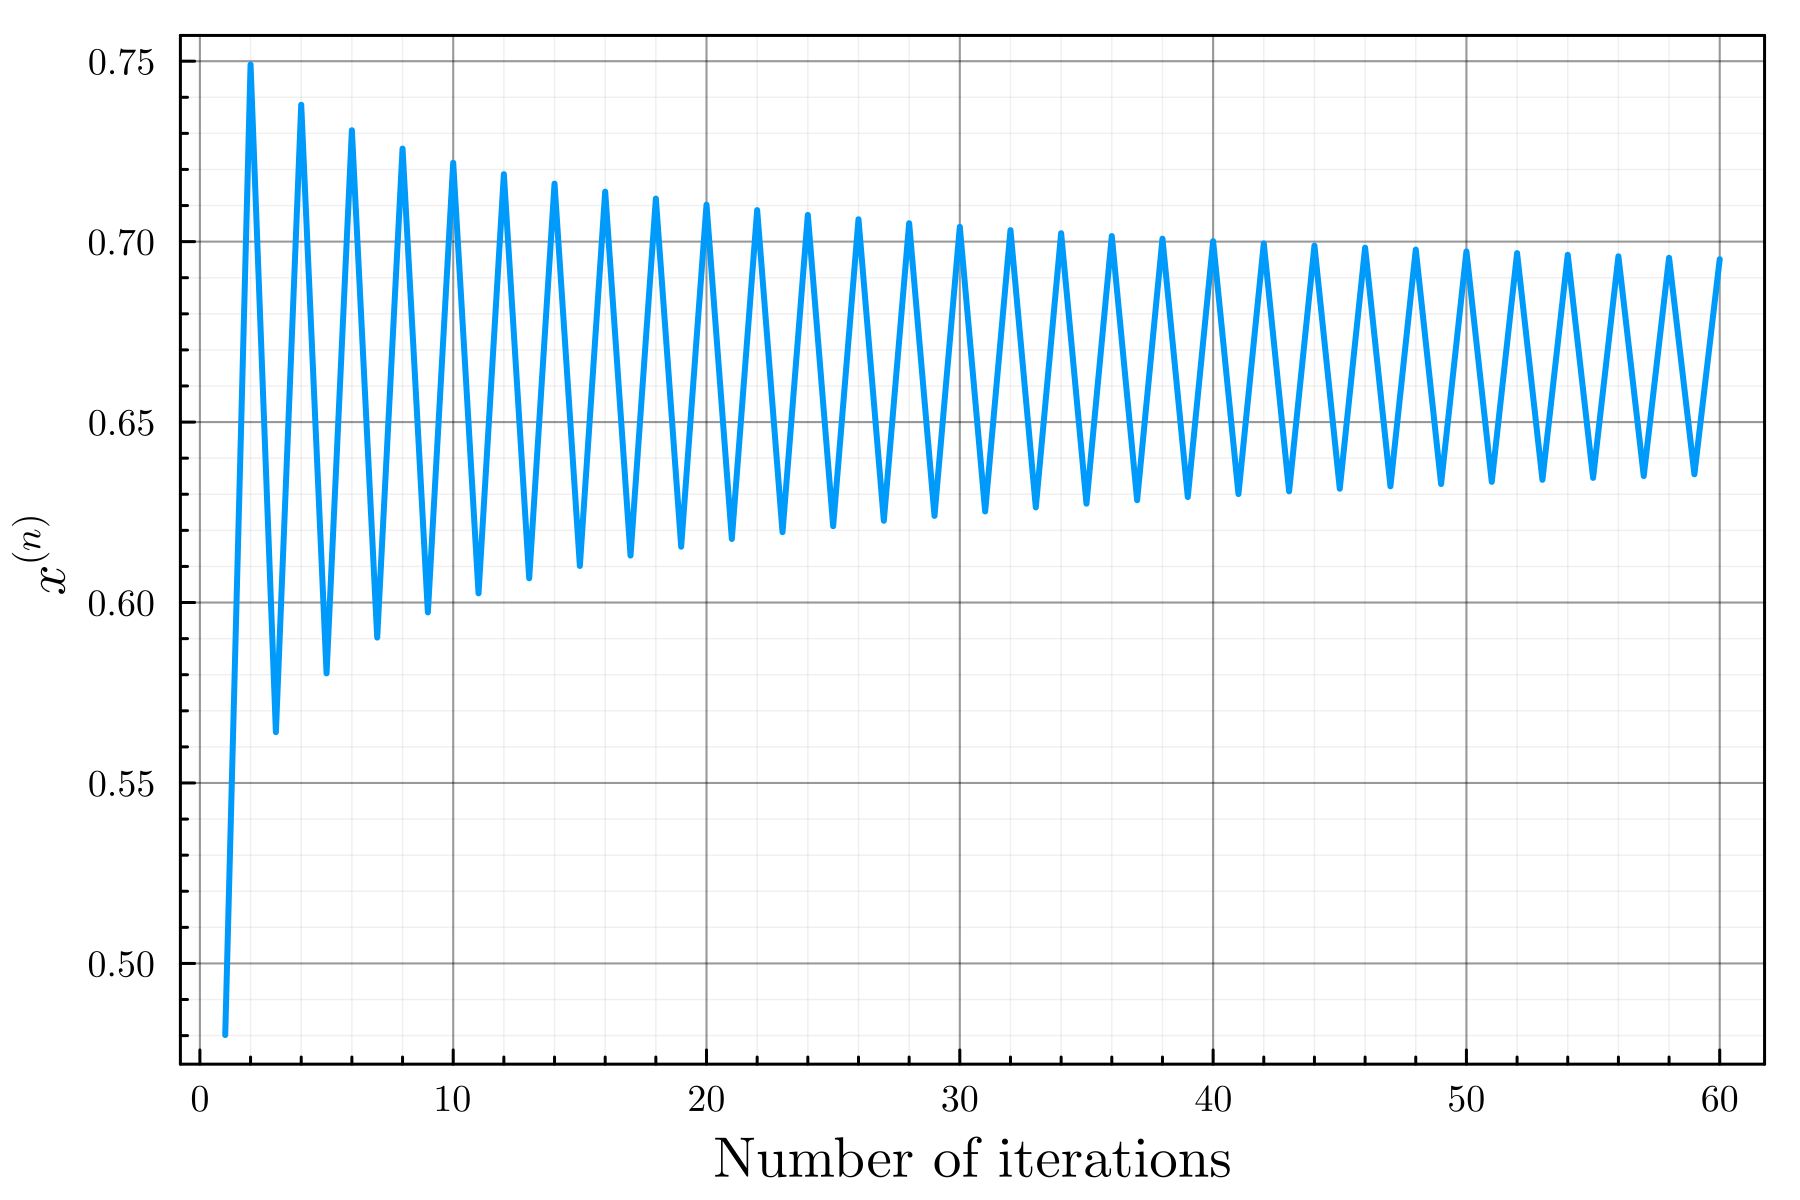
\includegraphics[width=\textwidth]{ch5/convergence_sublinear.png}
        \caption{Sub-linear convergence: $r = 3.001$}
    \end{subfigure}
    \caption{Convergence issues demonstrated using logistic map, $x^{(n+1)} = rx^{(n)}(1 - x^{(n)})$}
    \label{}
\end{figure}
%%% FIG %%%
\FloatBarrier \!\!\!\!\!\!\!\!\!\!\!

\subsection{No convergence}
This generally manifests in the form of 2-cycles. 
\begin{align*}
    f(\{\Psi_A, \Psi_B, \rho_A, \rho_B\}) = \{\Psi_A', \Psi_B', \rho_A', \rho_B'\}\\
    f(\{\Psi_A', \Psi_B', \rho_A', \rho_B'\}) = \{\Psi_A, \Psi_B, \rho_A, \rho_B\}    
\end{align*}

Every 2-cycle encountered also seems to have a pattern that can be exploited to guess the actual fixed point. For example:
\begin{align*}
    &\textbf{2-cycle: }(\Psi_A, \Psi_B, \rho_1, \rho_2) \rightarrow (\Psi_A, \Psi_B, \rho_2, \rho_1)\\
    &\textbf{Fixed point: } (\Psi_A, \Psi_B, (\rho_1 + \rho_2)/2, (\rho_1 + \rho_2)/2)        
\end{align*}

Several patterns like this can emerge, and one solution is to hard-code the guesses for fixed points for each case. This is unfortunately not scalable to arbitrary lattice geometries and parameter regimes. This problem arises from the strong dependancy on the initial guess for the self-consistency loop, and can be remedied by taking several initial guesses till one of them converges.

\subsection{Sub-linear convergence}
This manifests in a form that is decievingly similar to a 2-cycle.
$$f(\{\Psi_A, \Psi_B, \rho_A, \rho_B\}) \approx \{\Psi_A', \Psi_B', \rho_A', \rho_B'\}$$
$$f(\{\Psi_A', \Psi_B', \rho_A', \rho_B'\}) \approx \{\Psi_A, \Psi_B, \rho_A, \rho_B\}$$
The convergence happens at a very slow rate, especially close to the phase boundaries as seen in Fig. \ref{fig:converge_boundary}. This can be handled by utilizing more sophisticated techniques to locate the fixed point such as Nesterov's acceleration. 

%%% FIG %%%
\begin{figure}[!htb]
    \centering
    \begin{subfigure}[b]{0.45\textwidth}  %keep total sum <1 to show in same line
        \centering
        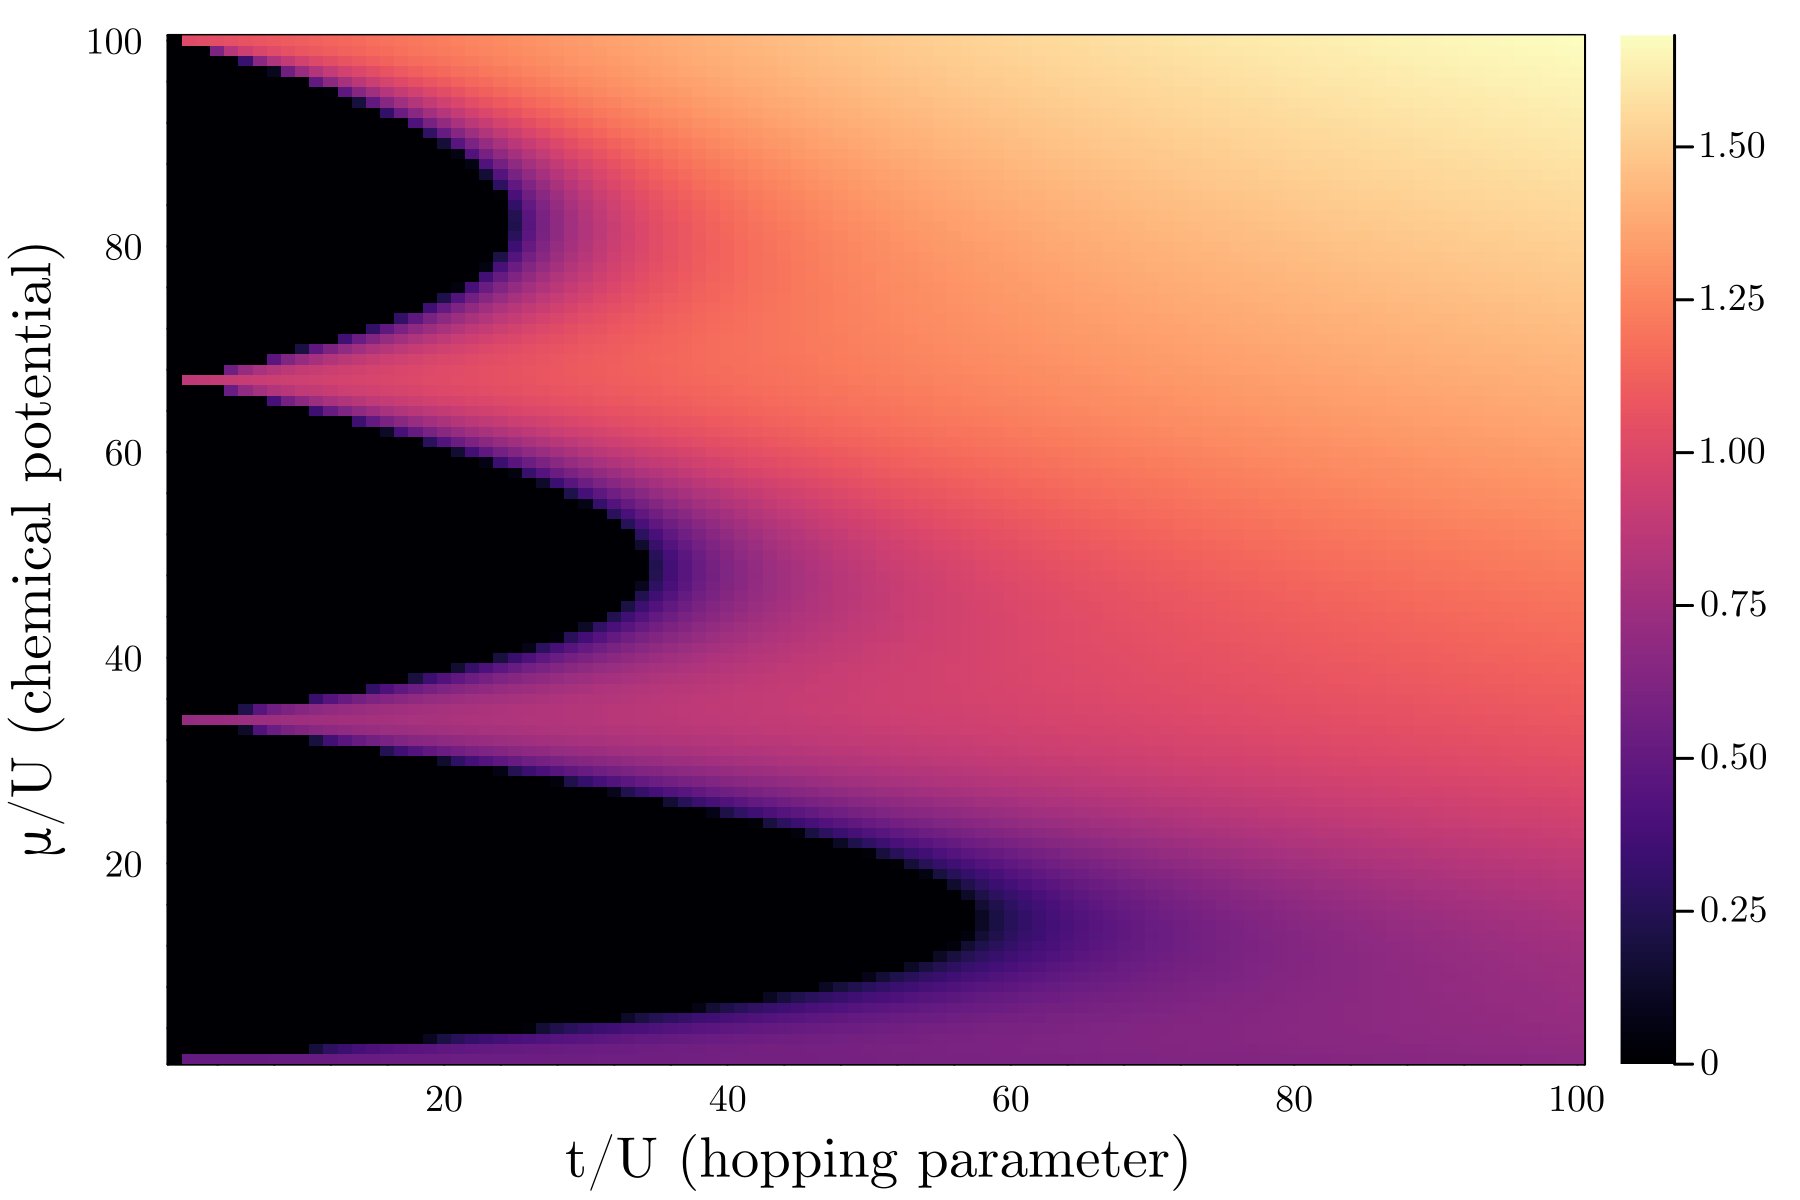
\includegraphics[width=\textwidth]{ch5/bhm_phasediagram.png}
        \caption{Order parameter}
    \end{subfigure}
    \hspace{1em}  %\hfill
    \begin{subfigure}[b]{0.45\textwidth}
        \centering
        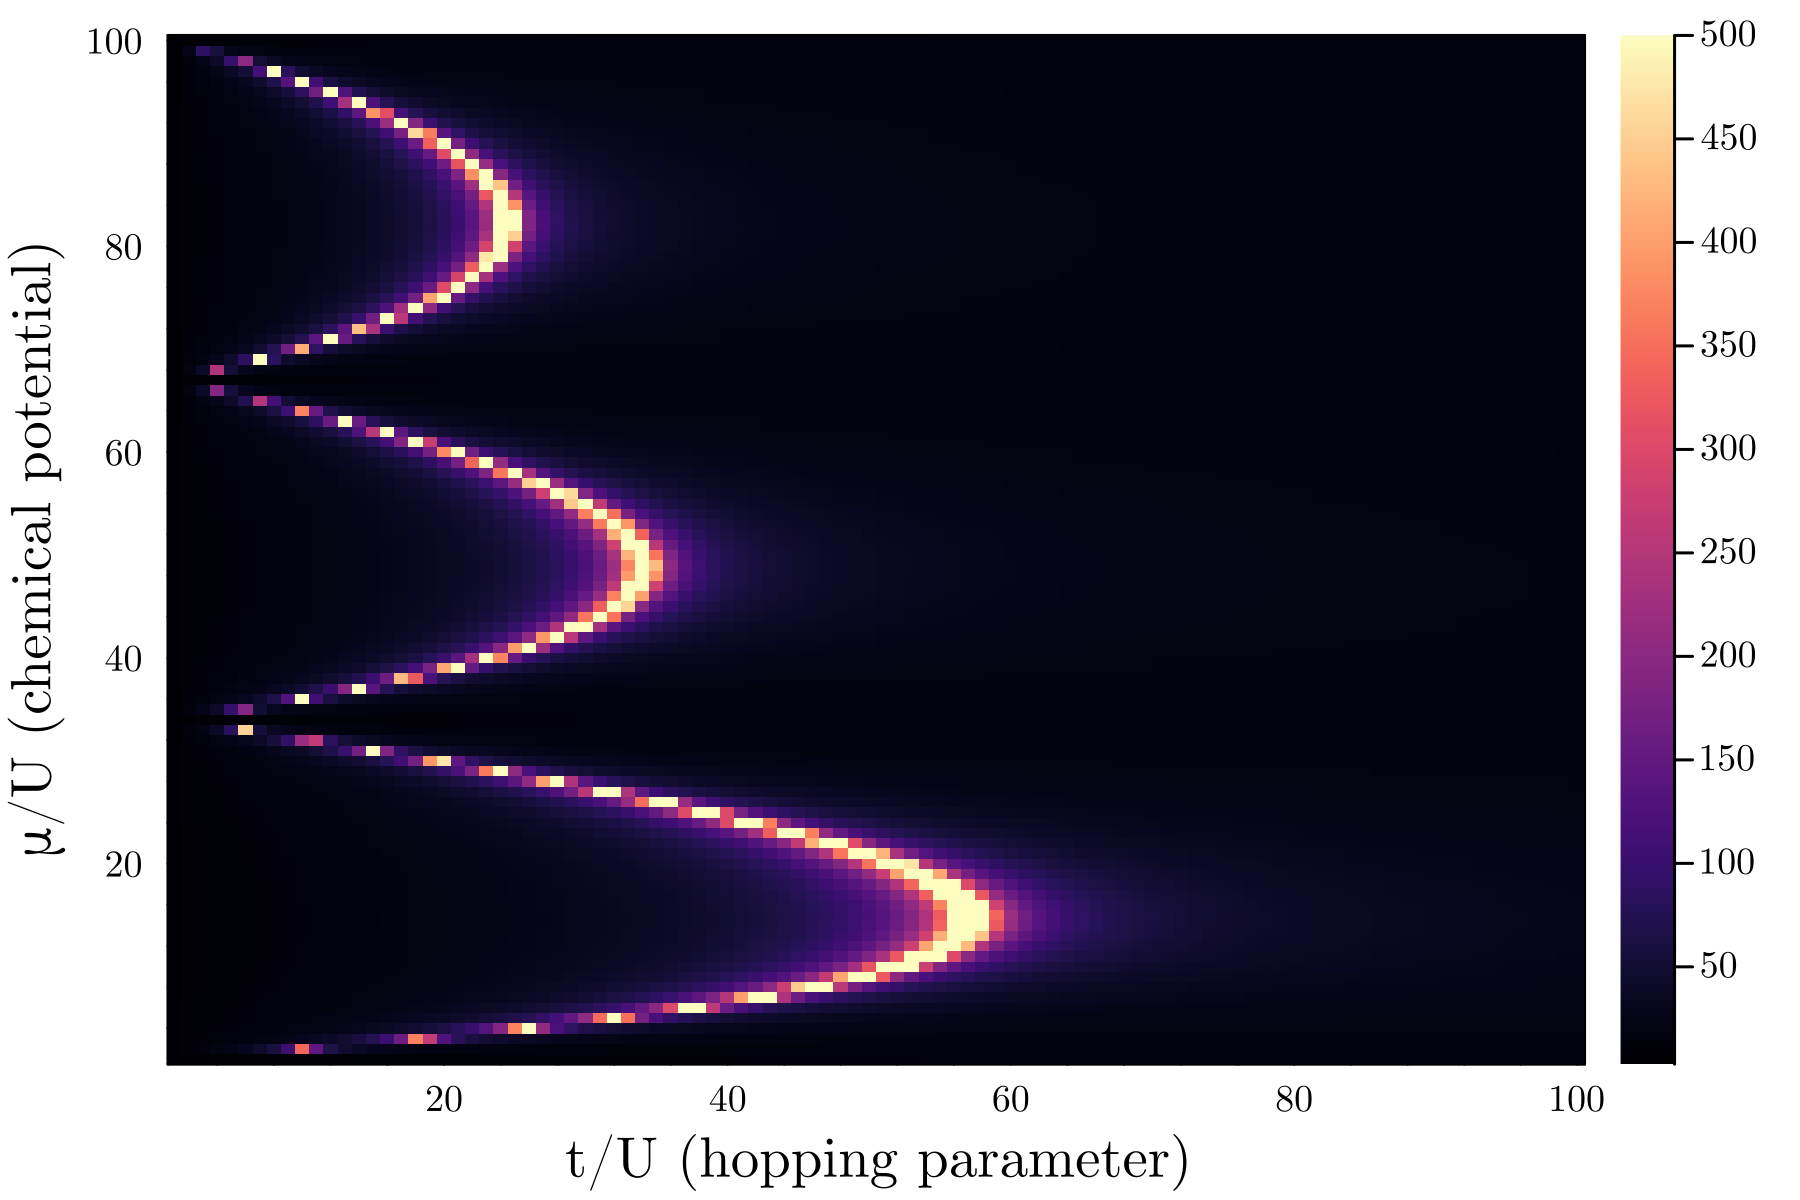
\includegraphics[width=\textwidth]{ch5/bhm_converge.png}
        \caption{Number of iterations}
    \end{subfigure}
    \caption{Nature of convergence near phase boundaries in the BHM}
    \label{fig:converge_boundary}
\end{figure}
%%% FIG %%%
\FloatBarrier \!\!\!\!\!\!\!\!\!\!\!

\subsection{Local minima}
Finally, we come to the important point that there may be several stable fixed points for the same system. By nature of the formulation of the mean-field technique, the true solution is the one with the lowest ground state energy. As a result, we are forced to perform self-consistency starting with a variety of initial guesses to avoid falling into local minima. There does not seem to be a simple way to sample the parameter space in an efficient manner to generate initial guesses. So, an arbitrarily chosen uniform grid was utilized for the results presented in this thesis, but this solution is hardly satisfactory.

\chapter{Spinful bosons in a lattice}\label{ch5}
In this chapter, we explore another form of short-ranged interaction, this time induced by spin-spin coupling. For this purpose, we will consider the simplest modification of the spinless case, which is the spin-1 Bose Hubbard model\cite{Tsuchiya_2004}. 
\begin{equation}
    H = -t\sum_{\langle i, j\rangle \sigma} a_{i\sigma}^{\dagger}a_{j\sigma} + \frac{U}{2}\sum_i n_i(n_i - 1) + V_s \sum_i (S_i^2 - 2n_i) - \mu \sum_i n_i
\end{equation}
The spin operators are determined as shown below, using the spin-1 matrices, $\{J_x, J_y, J_z\}$. 
\begin{equation}
    J_x = \frac{1}{\sqrt{2}}
    \begin{pmatrix}
    0 & 1 & 0 \\
    1 & 0 & 1 \\
    0 & 1 & 0
    \end{pmatrix}
    \hspace{0.5cm}
    J_y = \frac{i}{\sqrt{2}}\begin{pmatrix}
    0 & -1 & 0 \\
    1 & 0 & -1 \\
    0 & 1 & 0
    \end{pmatrix}
    \hspace{0.5cm}
    J_z = \begin{pmatrix}
    1 & 0 & 0 \\
    0 & 0 & 0 \\
    0 & 0 & -1
    \end{pmatrix}
\end{equation}
\begin{equation}
    \vec{S_i} = \sum_{\alpha \beta}a_{i\alpha}^{\dagger}\vec{J}_{\alpha \beta}a_{i\beta}
\end{equation}
Note that we have only taken into account the on-site interactions (due to contact scattering and spin-spin coupling). As a result, we do not expect to observe any fundamentally new phases besides the Mott insulator and superfluid. However, now that the bosons have an extra degree of freedom due to their spin ($S = 1, m_s \in \{1, 0, -1\}$), we expect some qualitative differences in the nature of these phases.

\section{Mean Field Theory}
The mean-field decoupling for the spin-1 BHM is is quite similar as for the spinless BHM since we have only introduced additional on-site interaction terms. However, we are now forced to introduce three mean-field parameters for each lattice site, one for each spin projection, $\hat{a}_{i\sigma} = \Psi_{i\sigma} + \delta \hat{a}_{i\sigma}$, where $\sigma \in \{1, 0, -1\}$. This gives us the decomposition of the hopping Hamiltonian as follows.
\begin{align}
    -H_{hop}/zt = \sum_{i\sigma} (\overline{\Psi}_{i\sigma} a_{i\sigma}^{\dagger} + \overline{\Psi}_{i\sigma}^* a_{i\sigma} - \overline{\Psi}_{i\sigma}\Psi_{i\sigma}^*)
\end{align}
As usual, we can assume translational invariance in the ground state and set $\Psi_{i\sigma} = \Psi_{\sigma} \hspace{0.1cm} \forall i$. We will also set $\Psi_{\sigma} \in \mathbb{R}$ for now, but will revisit this assumption further below. The spin-1 BHM can now be written as a sum over single-site Hamiltonians.
\begin{equation}
    H_i\{\Psi_{i\sigma}\} = -zt\sum_{\sigma}(\Psi_{i\sigma} a_{i\sigma}^{\dagger} + \Psi_{i\sigma}^* a_{i\sigma} - \Psi_{i\sigma}\Psi_{i\sigma}^*) + \frac{U_s}{2}(S_i^2 - 2n_i) + \frac{U}{2}n_i(n_i - 1) - \mu n_i
\end{equation}

The spin interaction term can be explicitly computed in terms of the creation/annihilation operators as shown below (where we have introduced the spin index $\overline{1}$ instead of $-1$ for notational clarity).
\begin{equation}
    \begingroup
    \renewcommand*{\arraystretch}{1.5}
    \begin{pmatrix}
        S_x \\
        S_y \\ 
        S_z
    \end{pmatrix}
    \endgroup = 
    \begingroup
    \renewcommand*{\arraystretch}{1.5}
    \begin{pmatrix}
        \frac{1}{\sqrt{2}}(a_{i1}^{\dagger}a_{i0} + a_{i0}^{\dagger}a_{i1} +a_{i\overline{1}}^{\dagger}a_{i0} + a_{i0}^{\dagger}a_{i\overline{1}}) \\ 
        \frac{i}{\sqrt{2}}(-a_{i1}^{\dagger}a_{i0} + a_{i0}^{\dagger}a_{i1} + a_{i\overline{1}}^{\dagger}a_{i0} - a_{i0}^{\dagger}a_{i\overline{1}})\\
        n_{i1} - n_{i\overline{1}}
    \end{pmatrix}
    \endgroup
\end{equation}
\begin{equation}
    S_i^2 = 2n_{i1}n_{i0} + 2n_{i0}n_{i\overline{1}} - 2n_{i1}n_{i\overline{1}} + n_{i1} + 2n_{i0} + n_{i\overline{1}} + n_{i1}^2 + n_{i\overline{1}}^2 + 2a_{i1}^{\dagger}a_{i\overline{1}}^{\dagger}a_{i0}^2 + 2(a_{i0}^{\dagger})^2a_{i1}a_{i\overline{1}}
\end{equation}
Note that most of the terms in the $S_i^2$ operator are block-diagonal in the spin subspaces except for the last two terms which mix the spin components. We can now construct the mean-field Hamiltonian in the occupation basis, $\ket{n_1, n_0, n_{\overline{1}}}$ resulting in the following ansatz for the wavefunction.
\begin{equation}
    \ket{\Psi} = \bigotimes_{i = 1}^M \left (\sum_{n_1, n_0, n_{\overline{1}}} f_{i, n_1, n_0, n_{\overline{1}}} \ket{n_1, n_0, n_{\overline{1}}} \right )
\end{equation}

\subsection{Mott insulator phase}\label{sec:mi_constraint}
When the order parameters satisfy $\Psi_1 = \Psi_0 = \Psi_{\overline{1}} = 0$, the ground state is a Mott insulator. In this section, we will try to understand the nature of the Mott insulator lobes due to the introduction of the spin degree of freedom, by considering the Hamiltonian in the limit $t \ll U$. 
\begin{equation}
    H_i = \frac{U_s}{2}(S_i^2 - 2n_i) + \frac{U}{2}n_i(n_i - 1) - \mu n_i
\end{equation}
The ground state would clearly be a Fock state with a fixed total occupation number, $n_i$ such that it is a superposition of spin states ($\sum_{\sigma}n_{i\sigma} = n_i$). However, note that $S_i^2$, $S_{iz}$ and $n_i$ commute with each other. As a result, a better basis for our analysis is the combined spin basis, $\ket{n_i; S_i, m_i}$ which is defined by the following eigenvalue equations.
\begin{align}
    \hat{S}_i^2 \ket{n_i; S_i, m_i} &= S_i(S_i + 1)\ket{n_i; S_i, m_i} \\  
    \hat{S}_{iz}\ket{n_i; S_i, m_i} &= m_i \ket{n_i; S_i, m_i} \\ 
    \hat{n}_i \ket{n_i; S_i, m_i} &= n_i \ket{n_i; S_i, m_i}
\end{align}
We can then write the ground state energy for the state $\ket{n; S, m}$ as follows.
\begin{equation}
    E(S, n) = \frac{U_s}{2}(S(S+1) - 2n) + \frac{U}{2}n(n+1) - \mu n
\end{equation}
Before we can determine the state $\ket{n;S, m}$, we must discuss the constraints on these quantum numbers. We will loosely follow the arguments presented in Ying (1996)\cite{ying96}. To begin with, we write the form of the spin ladder operators.
\begin{equation}
    S_+ = S_x + iS_y = \sqrt{2}(a_{1}^{\dagger}a_{0} + a_{0}^{\dagger}a_{\overline{1}}) \hspace{1cm} S_- = S_x - iS_y = \sqrt{2}(a_{0}^{\dagger}a_{1} + a_{\overline{1}}^{\dagger}a_{0})
\end{equation}
Since the spin operators obey the $SU(2)$ commutation relations, $[S_{i\alpha}, S_{i\beta}] = i \epsilon_{\alpha\beta\gamma}S_{i\gamma}$, the ladder structure follows and we have $m \in \{0, \pm 1, \pm 2, \dots \pm S\}$, generating $2S+1$ states for a given value of $n$ and $S$. Let us now consider the state $\ket{n;S, -S}$ to determine the allowed values of $S$. Applying $S_z$ on this state gives us the following relations:
\begin{align}
    2n_1 &= (n - S) - n_0 \\
    2n_{\overline{1}} &= (n + S) - n_{0}
\end{align}
This tells us that $S \leq n$ and further, $(n+S)$ and $n_0$ must both either be even or odd. If we assume that they are odd, we can expand the state $\ket{n; S, -S}$ in the following way.
\begin{equation}
    \ket{\Psi} = \ket{n; S, -S} = \sum_{n_0} c_{n_0} \ket{n_0, \frac{n -n_0 +S}{2}, \frac{n - n_0 - S}{2}} = \sum_{n_0} c_{n_0} \ket{\Psi_{n_0}}   
\end{equation}
By construction, we know that $S_-\Psi = 0$. However, note that the first term $S_-\ket{\Psi_1}$ gives rise to a state having $n_0 = 0$ since $S_- \sim a_{\overline{1}}^{\dagger}a_0$. No other term arising from $S_-\Psi_i$ for odd $i\geq 3$ can generate such a state with $n_0 = 0$. Since the overall result must vanish, we conclude that $c_{1} = 0$. Similarly, by considering the subsequent terms, we can argue that $c_{i} = 0 \hspace{0.1cm} \forall i$.  As a result, $S_-\ket{\Psi} = 0 \implies \ket{\Psi} = 0$, but we know that $\ket{n;S, -S} \neq 0$ so $(N+L)$ cannot be odd. Such an argument fails when $n_0$ is even, since we can conclude $c_i = 0 \hspace{0.1cm} \forall  i \geq 2$ but the lowest order term vanishes under annihilation, so $c_0$ can be non-zero. Thus, we have the constraint that $(n+S)$ must be even. This means that if $n$ is even, $S \in \{0, 2, 4, \dots, n\}$ and if $n$ is odd, $S \in \{1, 3, 5, \dots, n\}$. We will see in the subsequent sections that this constraint directly affects the ground state and hence the phase diagram. 



\subsection{Superfluid phase}
To characterize the superfluid phase, we turn our attention to the set of mean-field parameters which can be grouped like so, $\Psi = (\Psi_1, \Psi_0, \Psi_{\overline{1}}) = \sqrt{n_s}(\eta_1, \eta_0, \eta_{\overline{1}})$, where $n_s = |\Psi|$ is the superfluid density and $\vec{\eta}$ is a normalized spinor. Naturally, when $n_s$ does not vanish, we observe a superfluid phase and can understand its magnetic properties using the average spin given by $\langle \vec{S} \rangle = \sum_{\alpha\beta}\eta_{\alpha}^* \vec{J}_{\alpha\beta}\eta_{\beta}$. Writing out the components, we get:
\begin{equation}
    \begingroup
\renewcommand*{\arraystretch}{1.5}
\begin{pmatrix}
    \langle S_x \rangle \\
    \langle S_y \rangle \\ 
    \langle S_z \rangle
\end{pmatrix}
\endgroup = 
\begingroup
\renewcommand*{\arraystretch}{1.5}
\begin{pmatrix}
    \sqrt{2}(\eta_1\eta_0 + \eta_{\overline{1}}\eta_0) \\ 
    0 \\
    \eta_1^2 - \eta_{\overline{1}}^2
\end{pmatrix}
\endgroup
\end{equation}
Notice that the $y$-component of the average spin vanishes. At this point, we must review our assumption that $\Psi_\sigma \in \mathbb{R}$. Generally, this is valid because the BHM is invariant under the $U(1)$ transformation, $a_i \to e^{i\theta}a_i$ and any phase carried by the order parameter, $\Psi$, can be shifted onto the operators. However, in the spin-1 case, we would like to set all three order parameters, $\Psi_{\sigma}$, to be real. 
\vspace{0.5cm}\\
This creates an issue since the BHM is only invariant under \textit{global} gauge transformations, whereas our order parameters might carry different phases for each spin component, resulting in the transformation $a_{i\sigma} \to e^{i\theta_{\sigma}} a_{i\sigma}$. It can be seen that the spin-1 BHM is invariant under such a transformation only if $\theta_1 + \theta_{\overline{1}} - 2\theta_0 = m\pi$ where $m \in \mathbb{Z}$, precisely due to the spin mixing components of $S^2$. We can still set $\Psi_{\sigma} \in \mathbb{R}$ but this manifests in constraining the spin components of the superfluid strictly to the $x-z$ plane. While this means that we have lost generality, the physics of the system still remains the same and we will continue with this assumption for the sake of simplicity.
\vspace{0.5cm}\\
Getting back to the average spin, a nicer quantity to work with is its magnitude squared.
\begin{align}
    |\langle S \rangle|^2 &= 2(\eta_1\eta_0 + \eta_{-1}\eta_0)^2 + (\eta_1^2 - \eta_{-1}^2)^2 \nonumber\\
    &= 2(\eta_1^2 \eta_0^2 + \eta_{-1}^2 \eta_0^2 + 2 \eta_0^2\eta_1\eta_{-1}) + \eta_1^4 + \eta_{-1}^4 - 2\eta_1^2 \eta_{-1}^2 \nonumber\\ 
    &= (1 - \eta_0^2)\eta_0^2 + (1 - (\eta_1^2 + \eta_{-1}^2))(\eta_1^2 + \eta_{-1}^2) + 4z^2\eta_1\eta_{-1} + \eta_1^4 + \eta_{-1}^4 - 2\eta_1^2 \eta_{-1}^2 \nonumber\\
    &= \eta_0^2 - \eta_0^4 + \eta_1^2 + \eta_{-1}^2 - (\eta_1^2 + \eta_{-1}^2)^2 + 4 \eta_0^2\eta_1\eta_{-1} + \eta_1^4 + \eta_{-1}^4 - 2\eta_1^2 \eta_{-1}^2 \nonumber\\
    &= 1 - \eta_0^4 + 4 \eta_0^2\eta_1\eta_{-1} - 4\eta_1^2\eta_{-1}^2 \nonumber\\
    &= (1 - (\eta_0^2 - \eta_1\eta_{-1})^2)
\end{align}
If we define the singlet operator as $\Theta_i = (a_{i0}^2 - 2a_{i1}a_{i\overline{1}})$, we can directly relate its expectation value to the average spin like so $|\langle S\rangle|^2 = 1 - |\langle \Theta \rangle|^2/n_s^2$. In the ground state, based on the sign of $U_s$, the energy is minimized by $|\langle S \rangle|^2 = 0$ or $|\langle S \rangle|^2 = 1$ corresponding to a 'polar' or 'ferro' superfluid respectively\cite{Tsuchiya_2004}.


\section{Results}
\subsection{Ferromagnetic interactions ($U_s < 0$)}
In this case, the energy is minimized when the net spin of the bosons is maximised. As a result, the superfluid is of 'ferro' nature and exhibits average spin $|\langle S \rangle|^2 = 1$. Similarly, in the Mott insulator phase, each site has a net spin of $S = N$, where $N$ is the number of bosons occupying the site in that Mott lobe. This is allowed by the constraint we obtained in Sec. \ref{sec:mi_constraint}. As a result, there is no qualitative difference in the phase boundaries as compared to the spinless case. Note that whenever we mention 'spin', we mean the quantum number $S$ and not the projection $m_s$. As a result, in the absence of an external magnetic field, the system is actually magnetically unordered. We see that the observations discussed here are in agreement with Fig. \ref{fig:ferro}.
%%% FIG %%%
\begin{figure}[!htb]
    \centering
    \begin{subfigure}[b]{0.49\textwidth}  %keep total sum <1 to show in same line
        \centering
        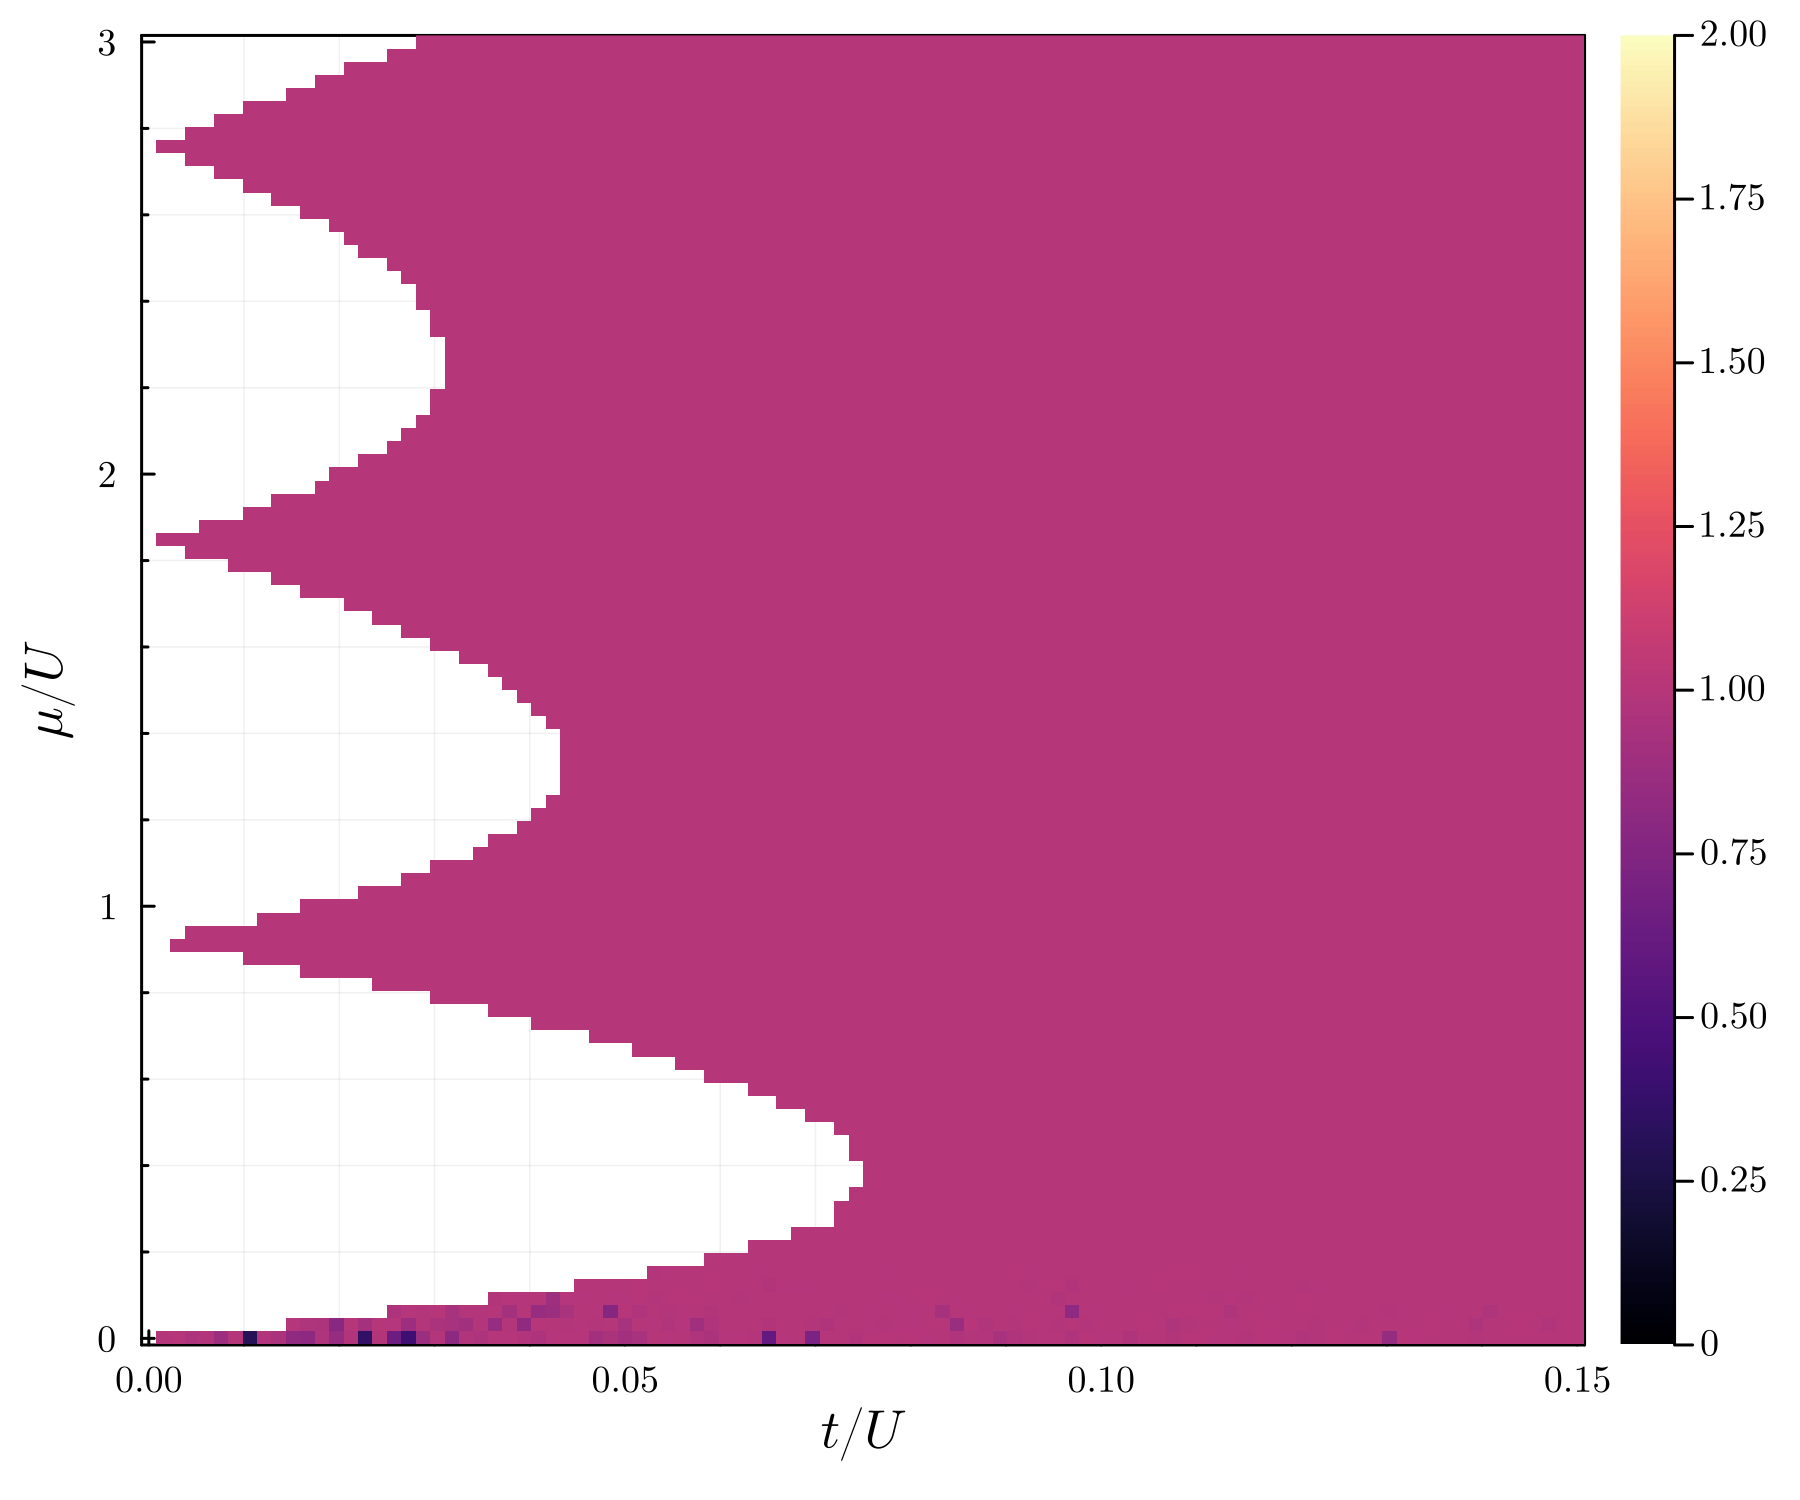
\includegraphics[width=\textwidth]{ch6/ferro_f.png}
        \caption{Average spin, $\langle \mathbf{S} \rangle$}
    \end{subfigure}
    \hspace{1em}  %\hfill
    \begin{subfigure}[b]{0.45\textwidth}
        \centering
        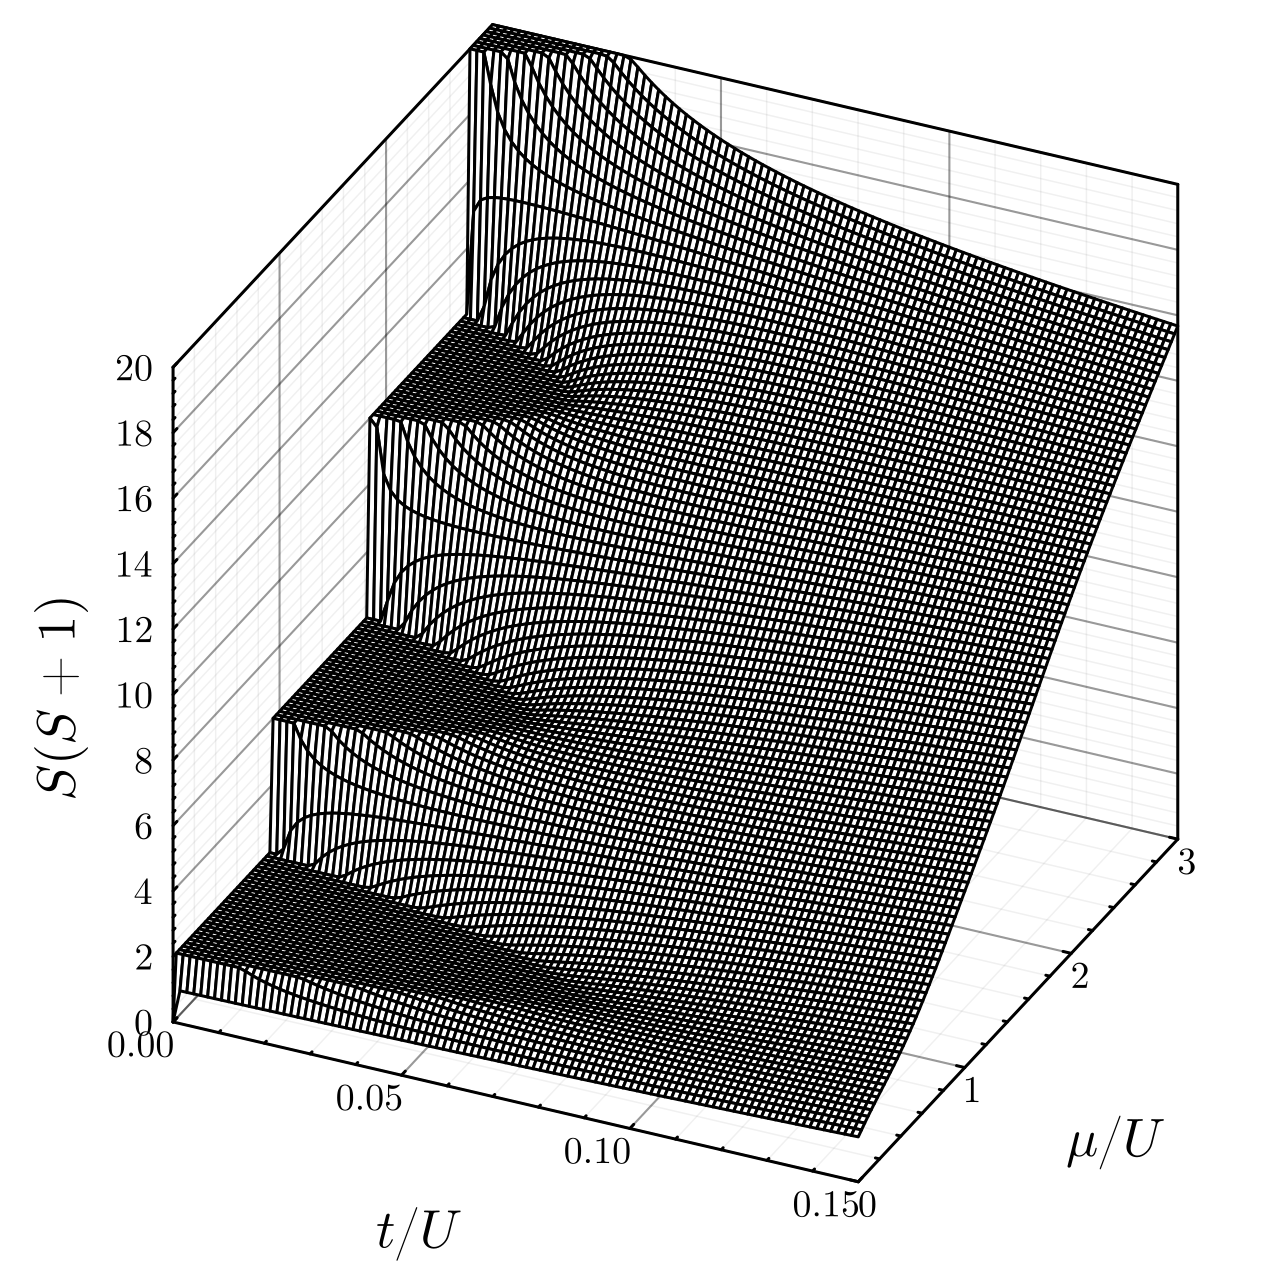
\includegraphics[width=\textwidth]{ch6/ferro_spin.png}
        \caption{Net spin eigenvalue, $\langle S^2 \rangle$}
    \end{subfigure}
    \hspace{1em}
    \vspace{0.5cm}  %\hfill
    \centering
    \begin{subfigure}[b]{0.75\textwidth}  %keep total sum <1 to show in same line
        \centering
        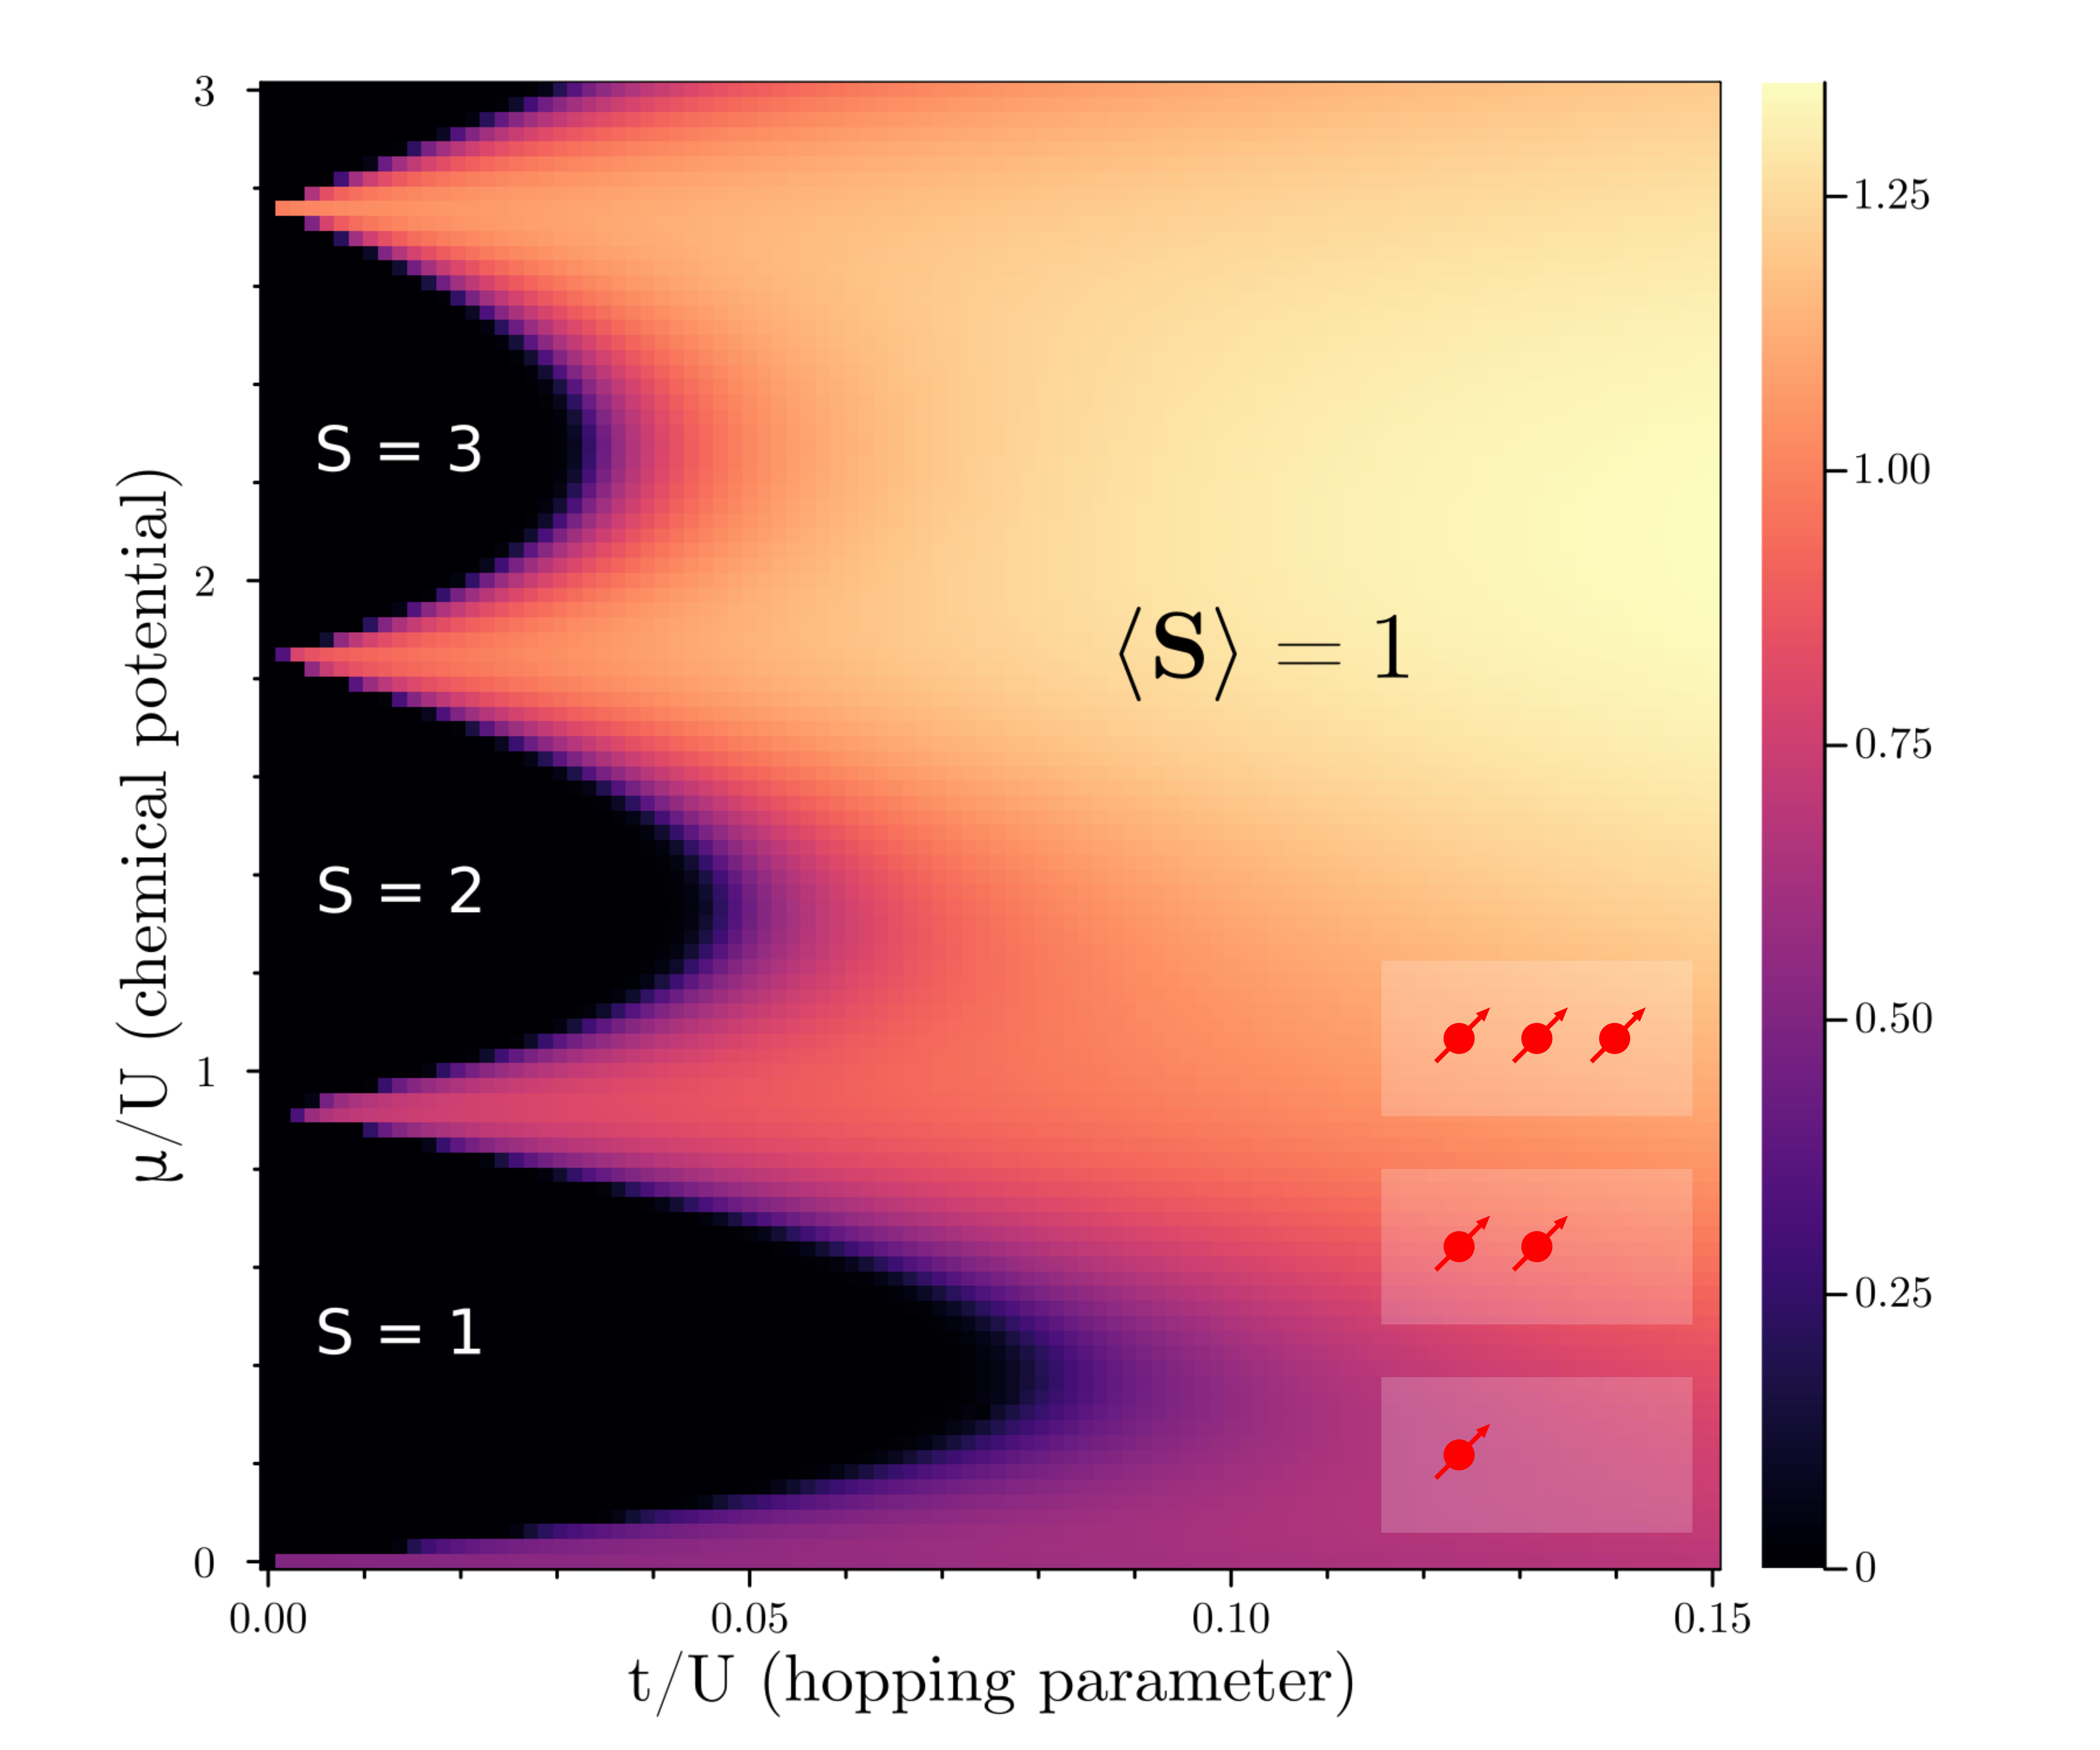
\includegraphics[width=\textwidth]{ch6/ferro_phases.png}
        \caption{Phase diagram}
    \end{subfigure}
    \caption{Ferromagnetic interactions, $U_s = -0.08U$}
    \label{fig:ferro}
\end{figure}
%%% FIG %%%
\FloatBarrier \!\!\!\!\!\!\!\!\!\!\!

\subsection{Anti-ferromagnetic interactions ($U_s > 0$)}

In this case, the energy is minimized when the net spin of the bosons is minimized. As a result, the superfluid is of 'polar' nature and exhibits average spin $|\langle S \rangle|^2 = 0$. Things get interesting in the Mott insulator phase, however, since the constraint from Sec. \ref{sec:mi_constraint} plays a bigger role now as we can see in Fig. \ref{fig:antiferro}. 
\vspace{0.5cm}\\
The Mott lobes with even $N$ is described by the state $\ket{N; 0, 0}$ with $N/2$ pairs of spin singlets, whereas the Mott lobes with odd $N$ is described by the state $\ket{N;1, m}$ such that there is one boson that cannot form a singlet. This has a direct effect on the phase boundaries since singlet formation stabilizes the Mott insulator against the superfluid transition\cite{Tsuchiya_2004}. As a result, there is significant difference in the phase boundary of this system as compared to the spinless case. Further, note that the SF-MI transition is generally second order in nature. However, in this case, only the SF-(odd) MI transitions are second order, while the SF-(even) MI transitions are first order in nature.  

\section{Effective spin-spin interactions}
While the mean-field decoupling allowed us to study the effect of the spin degree of freedom in the ordered phases of the BHM, it also threw away any correlations across the lattice. In the pure Mott insulator limit when $t \ll U$, such a treatment is accurate since the orientations of spins in different lattice sites are genuinely uncorrelated. However, as we introduce finite hopping, the bosons can mediate an interaction between the spins on different sites, thus introducing spin-spin correlations that can give rise to singlet and nematic ordering within the Mott lobes. 
\vspace{0.5cm}\\
In general, one can write an effective spin Hamiltonian for such a case\cite{Tsuchiya_2004}.
\begin{equation}
    H_{\text{eff}} = \sum_{\langle i, j\rangle} (-J_{i, j}^{(0)} - J_{i, j}^{(1)} S_i \cdot S_j - J_{i, j}^{(2)} (S_i \cdot S_j)^2)
\end{equation}
where the coefficients are determined by a perturbative treatment of the hopping term. However, we will not pursue this exercise here since the phenomenon of mediation is complicated by the presence of other terms in the spin-1 BHM. Instead, we study a simpler situation that demonstrates mediation more clearly in the next chapter.   

%%% FIG %%%
\begin{figure}[!htb]
    \centering
    \begin{subfigure}[b]{0.49\textwidth}  %keep total sum <1 to show in same line
        \centering
        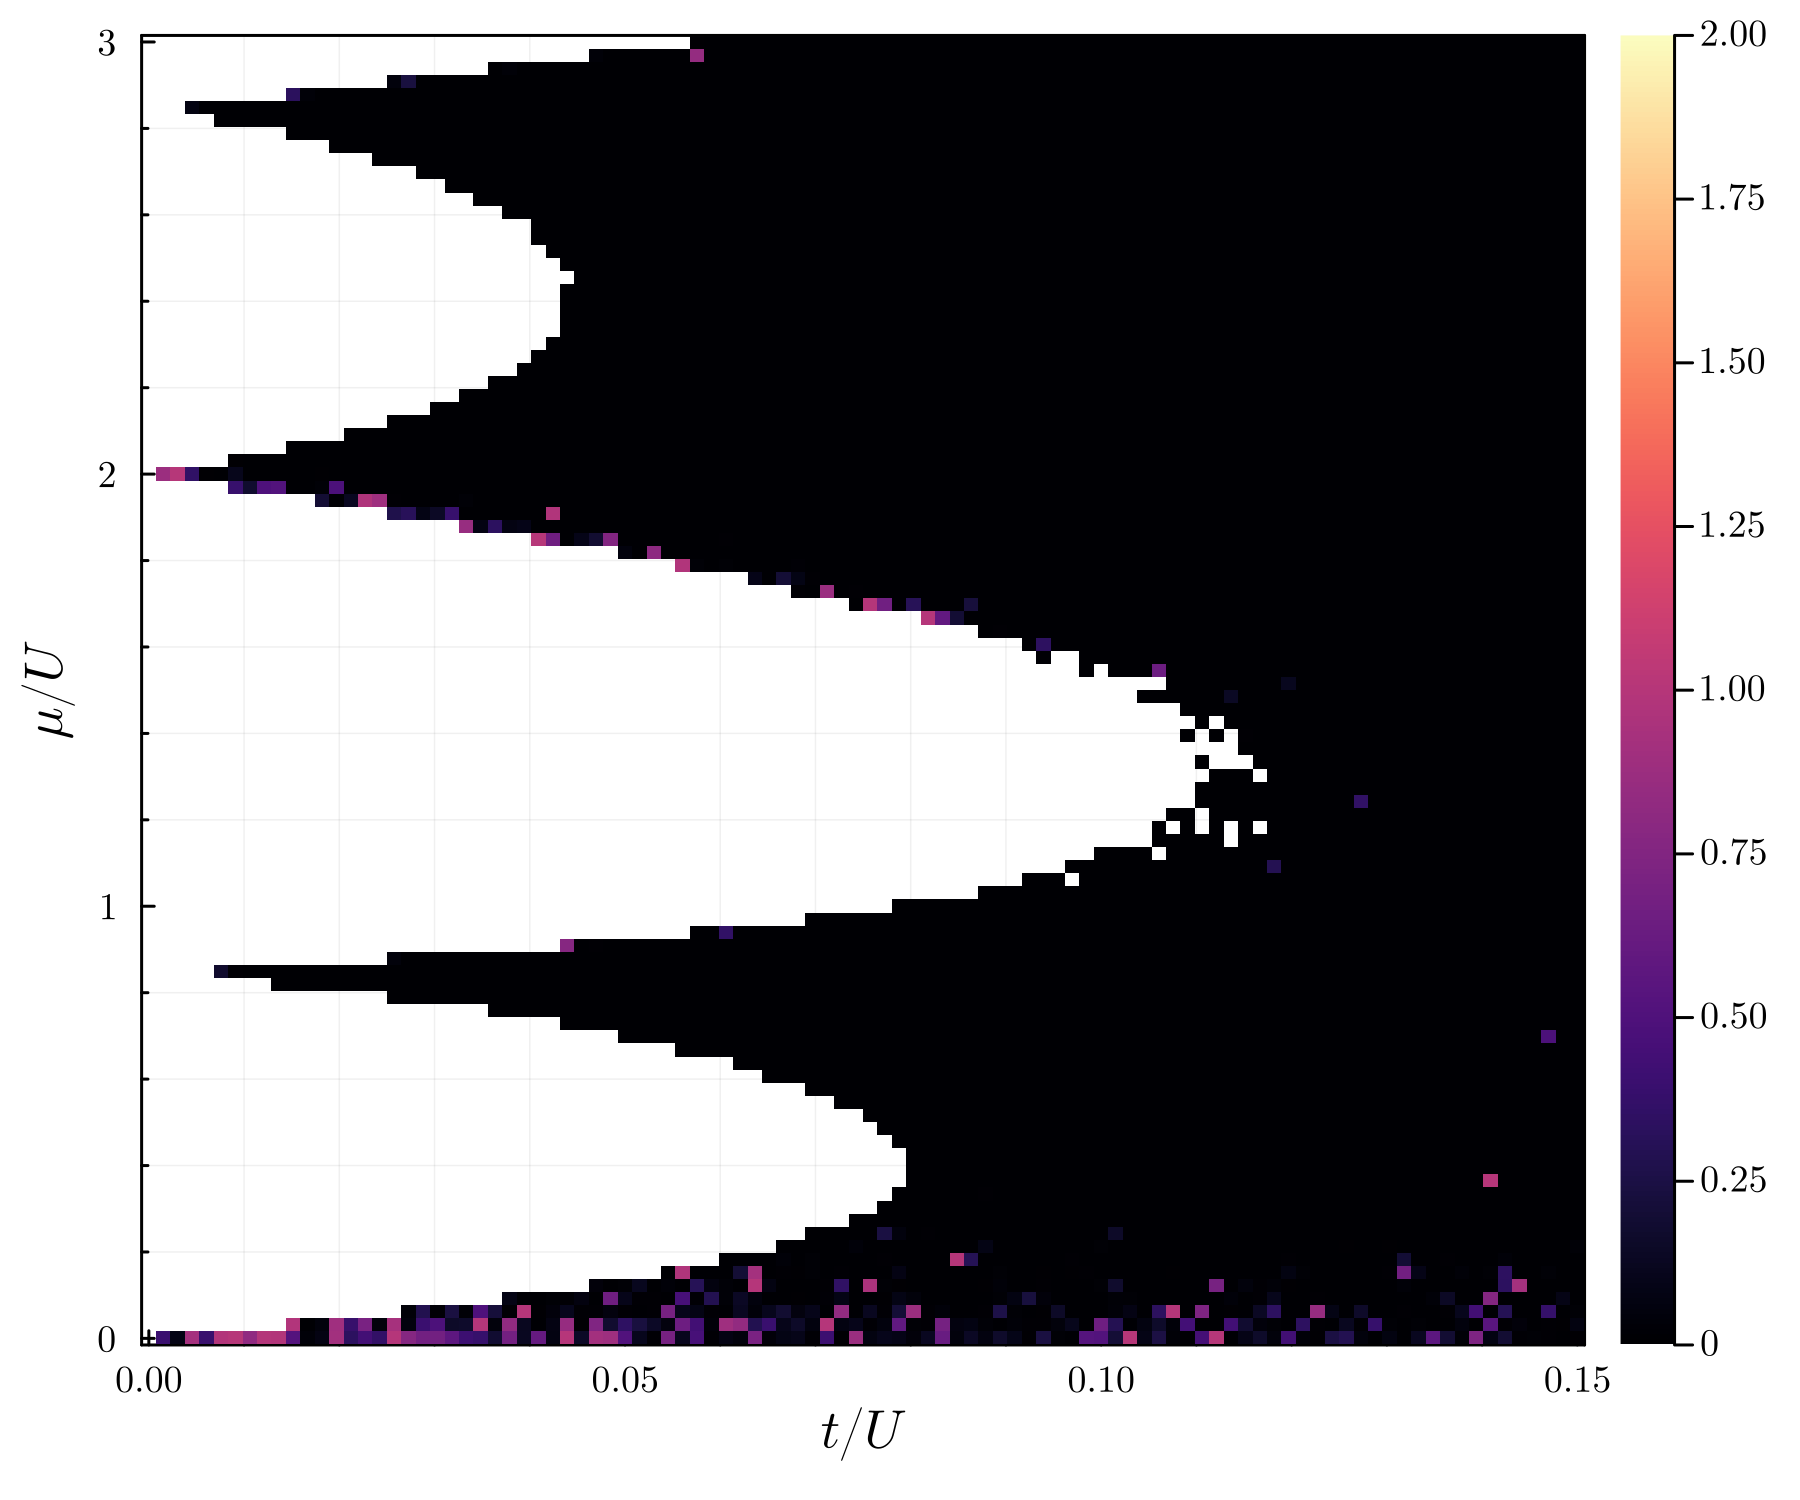
\includegraphics[width=\textwidth]{ch6/antiferro_f.png}
        \caption{Average spin, $\langle \mathbf{S} \rangle$}
    \end{subfigure}
    \hspace{1em}  %\hfill
    \begin{subfigure}[b]{0.45\textwidth}
        \centering
        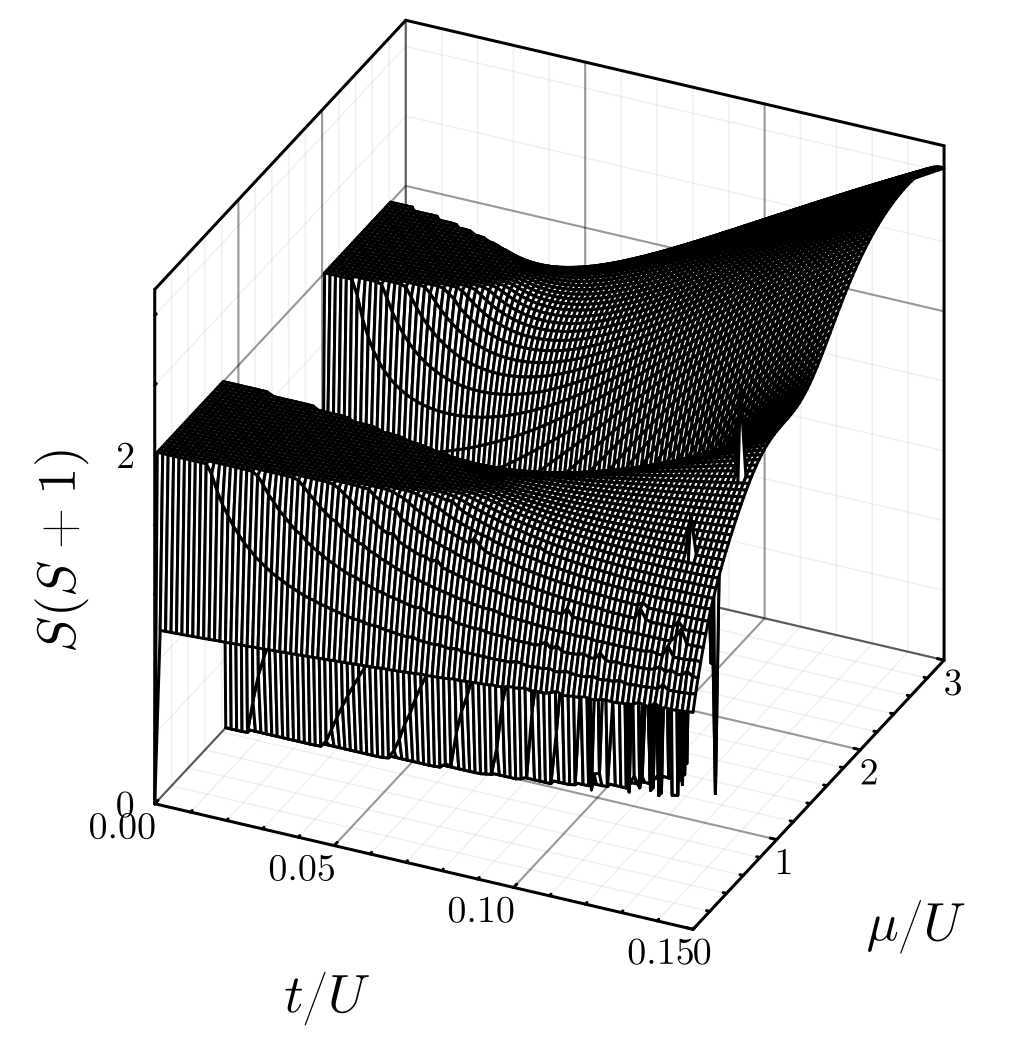
\includegraphics[width=\textwidth]{ch6/antiferro_spin.png}
        \caption{Net spin eigenvalue, $\langle S^2 \rangle$}
    \end{subfigure}
    \hspace{1em}
    \vspace{0.5cm}  %\hfill
    \centering
    \begin{subfigure}[b]{0.75\textwidth}  %keep total sum <1 to show in same line
        \centering
        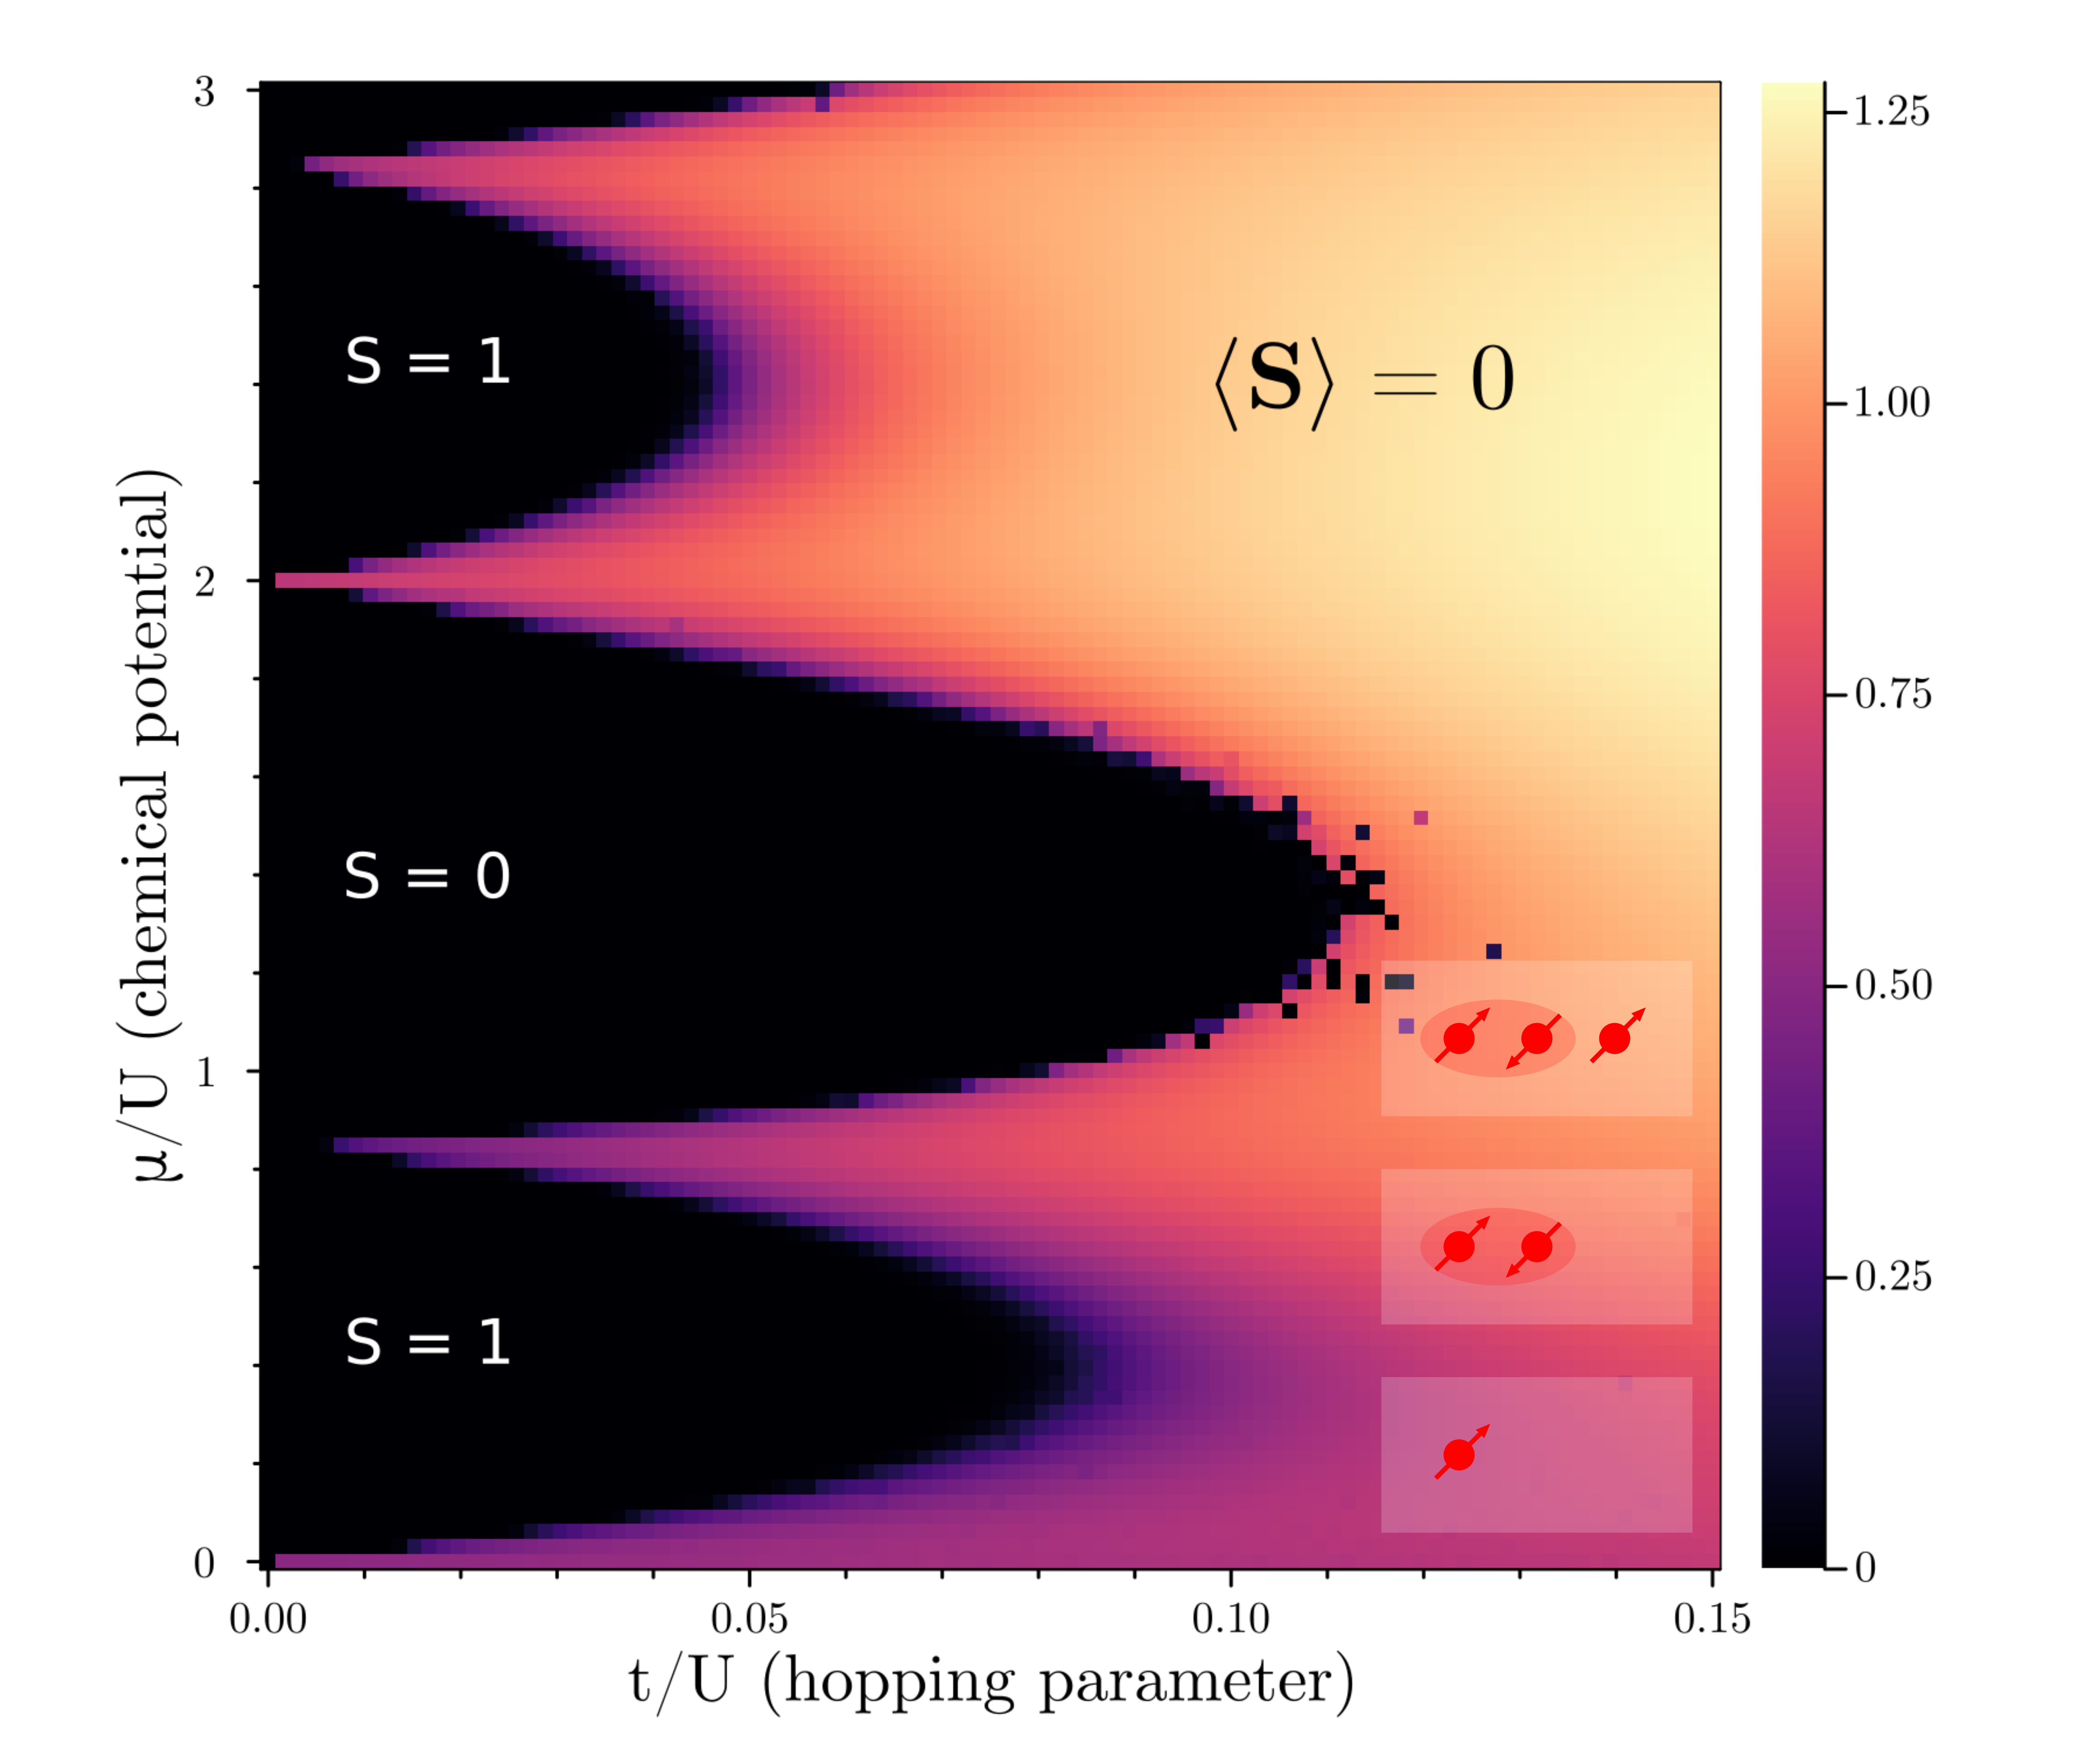
\includegraphics[width=\textwidth]{ch6/antiferro_phases.png}
        \caption{Phase diagram}
    \end{subfigure}
    \caption{Anti-ferromagnetic interaction, $U_s = 0.08U$}
    \label{fig:antiferro}
\end{figure}
%%% FIG %%%
% \FloatBarrier \!\!\!\!\!\!\!\!\!\!\!


\chapter{Boson-mediated interactions}\label{ch6}
In this chapter, we consider a simple model of non-interacting spin-1 bosons on a lattice coupled with a lattice of localized spin-1 bosonic 'impurities'. This can be seen as analogue of the fermionic lattice kondo model. Our goal is to explore the nature boson-mediated interactions. 
\begin{equation}
    H = -t\sum_{\langle i, j\rangle, \sigma} a_{i\sigma}^{\dagger}a_{j\sigma} - J_h \sum_i S_i \cdot s_i
\end{equation}
This model can be thought of arising from a more general one involving coupling between the lattice and impurity bosons, in the low-energy limit of single particle occupation in the impurity sites. As a result, the localized spins can be treated as classical spins such that $|\vec{S}_i| = 1$, parametrized like so $\vec{S}_i = (\cos\phi_i\sin\theta_i, \sin\phi_i\sin\theta_i, \cos\theta_i)$. Note that the localized spins do not directly interact with each other in this system.

\section{Strong-coupling limit}
%%% FIG %%%
\begin{figure}[!htb]
    \centering
    \begin{subfigure}[b]{\textwidth}  %keep total sum <1 to show in same line
        \centering
        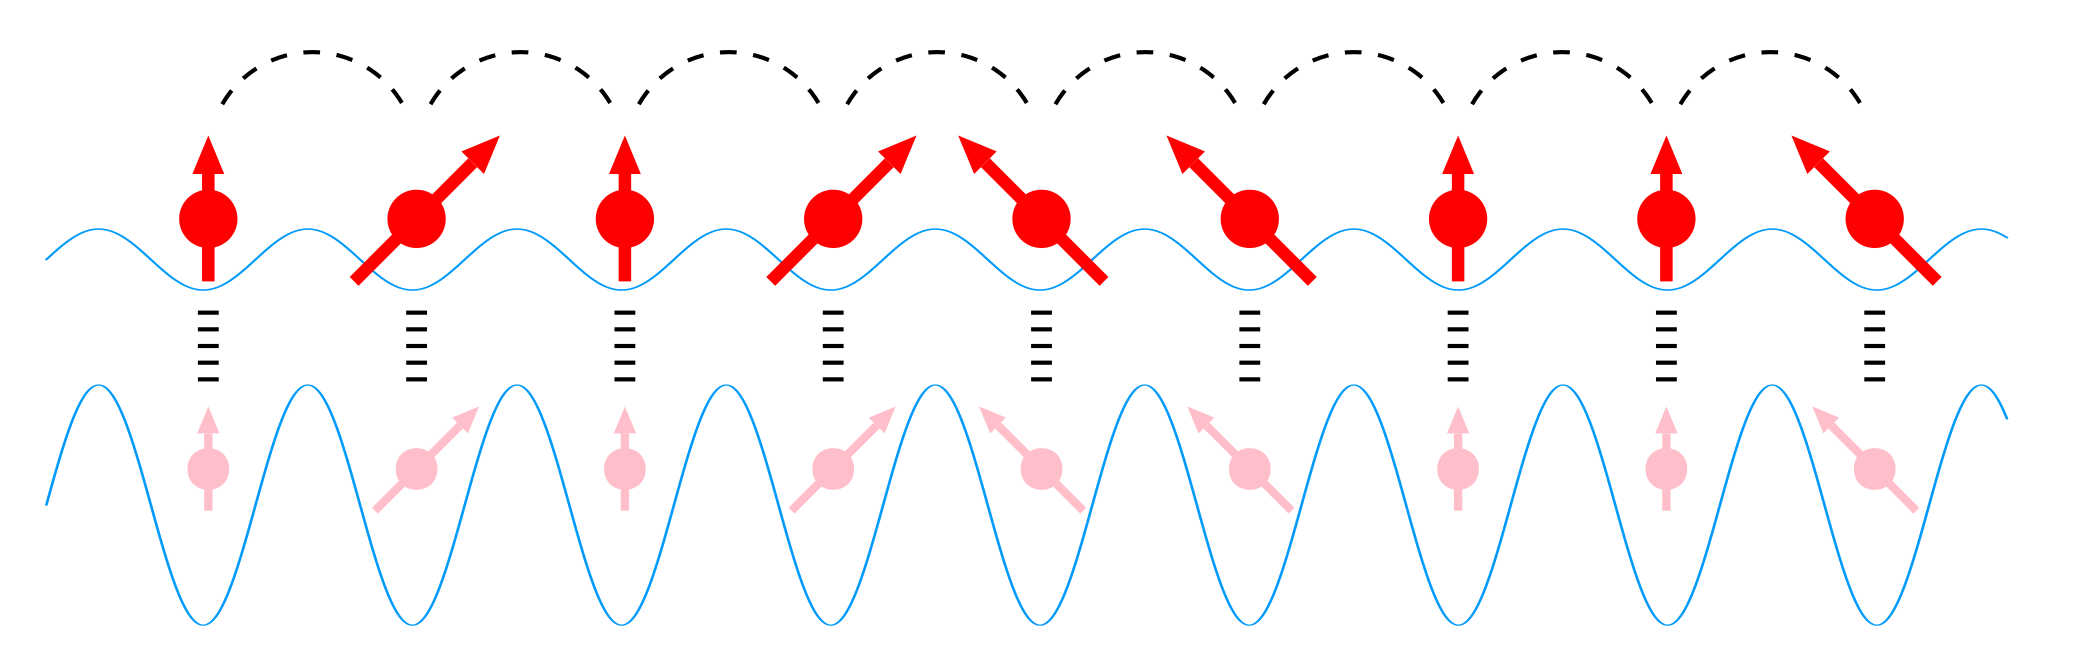
\includegraphics[width=\textwidth]{ch7/mediation.png}
    \end{subfigure}
    \caption{Conduction bosons (red) and impurity bosons (pink) confined in a lattice}
    \label{}
\end{figure}
%%% FIG %%%
\FloatBarrier \!\!\!\!\!\!\!\!\!\!\!

Let us consider the limit $J_h \gg t$ wherein the bosons have a strong tendency to align with the classical spins. This motivates us to change our basis by applying a site-dependant $SU(2)$ rotation (see Appendix \ref{app:rotation}).

\begin{equation}
    \begin{bmatrix}
        a_{i, 1} \\
        a_{i, 0} \\ 
        a_{i, \overline{1}}
    \end{bmatrix} = 
    \begin{bmatrix}
        \cos^2\frac{\theta_i}{2} & -\frac{1}{\sqrt{2}} \sin\theta_i e^{-i\phi_i} & \sin^2\frac{\theta_i}{2}e^{-2i\phi_i} \\ 
        \frac{1}{\sqrt{2}} \sin\theta_i e^{i\phi_i} & \cos\theta_i & -\frac{1}{\sqrt{2}} \sin\theta_i e^{-i\phi_i} \\
        \sin^2\frac{\theta_i}{2}e^{2i\phi_i} & \frac{1}{\sqrt{2}} \sin\theta_i e^{i\phi_i} & \cos^2\frac{\theta_i}{2}
    \end{bmatrix}
    \begin{bmatrix}
        d_{i, 1} \\
        d_{i, 0} \\ 
        d_{i, \overline{1}}  
    \end{bmatrix}
\end{equation}
The new operator, $d_{i, \sigma}$, annihilates a boson at site $i$ with the spin $\sigma \in [1, 0, \overline{1}]$ such that the quantization axis is now parallel to the localized spin. The transformed Hamiltonian can then be written as follows.
\begin{equation}
    H = \underbrace{\sum_{\langle i, j\rangle \sigma \sigma'}g_{ij}^{\sigma \sigma'} d_{i\sigma}^{\dagger} d_{j\sigma'}}_{V} - \underbrace{J_H\sum_i (n_{i,1} - n_{i, \overline{1}})}_{H_0}
\end{equation}
where $n_{i, \sigma}$ are the defined by $d_{i, \sigma}^{\dagger} d_{i, \sigma}$. Note that this transformation effectively diagonalizes the spin coupling term, which allows us to treat the hopping term in a perturbative manner. Although the elements of the new hopping matrix are not particularly insightful, they are listed below (as a multiple of $t_{i, j}$) for completeness.

\begin{align*}
    g_{i, j}^{1, 1} &= \cos^2 \frac{\theta_i}{2} \cos ^2  \frac{\theta_j}{2}  + \frac{1}{2}e^{-i(\phi_i - \phi_j)}\sin\theta_i\sin\theta_j + e^{-2i(\phi_i - \phi_j)}\sin^2 \frac{\theta_i}{2} \sin^2 \frac{\theta_j}{2}\\
%
    g_{i, j}^{1, 0} &= \frac{1}{\sqrt{2}}e^{-i\phi_i}\sin\theta_i\cos\theta_j - \frac{1}{\sqrt{2}}e^{-i\phi_j}\cos^2\frac{\theta_i}{2}  \sin\theta_j + \frac{1}{\sqrt{2}}e^{-i(2\phi_i - \phi_j)} \sin ^2  \frac{\theta_i}{2} \sin\theta_j\\
%    
    g_{i, j}^{1, \overline{1}} &=  e^{-2i\phi_i} \cos^2\frac{\theta_j}{2}\sin^2\frac{\theta_i}{2} + e^{-2i\phi_j}\cos^2\frac{\theta_i}{2}\sin^2\frac{\theta_j}{2} - \frac{1}{2}e^{-i(\phi_i + \phi_j)}\sin\theta_i\sin\theta_j\\
%   
    g_{i, j}^{0, 0} &=  \cos\theta_i\cos\theta_j + \frac{1}{2}e^{i(\phi_i - \phi_j)}\sin\theta_i\sin\theta_j + \frac{1}{2}e^{-i(\phi_i - \phi_j)}\sin\theta_i\sin\theta_j \\
%    
    g_{i, j}^{0, \overline{1}} &=  \frac{1}{\sqrt{2}}e^{-i\phi_i}\cos^2\frac{\theta_j}{2}\sin\theta_i - \frac{1}{\sqrt{2}}e^{-i\phi_j}\cos\theta_i\sin\theta_j - \frac{1}{\sqrt{2}}e^{-i(-\phi_i + 2\phi_j)}\sin\theta_i\sin^2\frac{\theta_j}{2}\\
%    
    g_{i, j}^{\overline{1}, \overline{1}} &= \cos^2\frac{\theta_i}{2}\cos^2\frac{\theta_j}{2} + \frac{1}{2}e^{i(\phi_i - \phi_j)}\sin\theta_i\sin\theta_j + e^{2i(\phi_i - \phi_j)}\sin^2\frac{\theta_i}{2}\sin^2\frac{\theta_j}{2}
\end{align*}

The remaining elements can be computed by using the property $g_{i, j}^{\sigma, \sigma'} = (g_{j, i}^{\sigma', \sigma})^*$. These coefficients can be understood as the spin-spin coupling resulting in an effective (reduced) hopping term. Let us now consider a simple case of unit occupation on the lattice, and further, we restrict the analysis to a two-site problem. The ground state for the unperturbed system is then triply degenerate.
$$\ket{0, 2} = d_{2, 1}^{\dagger}d_{2, 1}^{\dagger}\ket{0} \hspace{1cm} \ket{2, 0} = d_{1, 1}^{\dagger}d_{1, 1}^{\dagger}\ket{0}\hspace{1cm}\ket{1, 1} = d_{2, 1}^{\dagger}d_{1, 1}^{\dagger}\ket{0}$$

with energy $E_0^{(0)} = -2J_h$. Since the ground state is degenerate, we must diagonalize $V$ within this subspace to calculate the first order correction to the ground state energy. The details to compute the vacuum expectation values can be found in Appendix \ref{app:wick}. We can then write the matrix elements of $V$ in this subspace as follows.
\begin{equation}
    \bra{l, l'}V\ket{m,m'} = g_{m'l'}^{1,1} \delta_{lm} + g_{m'l}^{1,1}\delta_{l'm} + g_{ml'}^{1,1}\delta_{lm'} + g_{ml}^{1,1} \delta_{l'm'}
\end{equation}

\begin{equation}
    V = 2\Re
\begingroup
\renewcommand*{\arraystretch}{1.5}
\begin{pmatrix}
    g_{1,1}^{1,1} + g_{2, 2}^{1, 1} & 2 g_{1, 2}^{1, 1} & 2g_{2, 1}^{1, 1}\\
    2 g_{1, 2}^{1, 1} & 4t_{1, 1}^{1, 1} & 0 \\
    2g_{2, 1}^{1, 1} & 0 & 4g_{2,2}^{1, 1}
\end{pmatrix}
\endgroup
= 4
\begingroup
\renewcommand*{\arraystretch}{1.5}
\begin{pmatrix}
    0 & \Re(g_{1, 2}^{1, 1}) & \Re((g_{1, 2}^{1, 1})^*)\\
    \Re(g_{1, 2}^{1, 1}) & 0 & 0 \\
    \Re((g_{1, 2}^{1, 1})^*) & 0 & 0
\end{pmatrix}
\endgroup
\end{equation}
The smallest eigenvalue is the first order correction, $E_0^{(1)}=-4\sqrt{2}\Re(g_{1, 2}^{1, 1})$, giving us the following expression.
\begin{align}
E_0^{(1)}(\theta_i, \phi_i, \theta_j, \phi_i) = -4\sqrt{2}t_{i, j}&\left [ \cos^2\frac{\theta_i}{2}\cos^2\frac{\theta_j}{2} + \frac{1}{2}\cos(\phi_i - \phi_j)\sin\theta_i \sin\theta_j \right . \nonumber\\
&\left .+ \cos(2(\phi_i - \phi_j))\sin^2\frac{\theta_i}{2}\sin^2\frac{\theta_j}{2}\right ]    
\end{align}

Note that we have 'integrated out' the bosonic part of the system and ended up with an expression for the corrected energy purely in terms of the components of the localized spins. Thus, we have $H_{\text{eff}}({\theta_i, \phi_i, \theta_j, \phi_j}) = E_0^{(1)}(\theta_i, \phi_i, \theta_j, \phi_j) + E_0^{(0)}$ as an effective Hamiltonian governing the physics of the localized spins. We can also clearly see that the two spin variables are coupled in a non-trivial manner, thereby acting as an effective interaction that is mediated by the lattice bosons! 
\vspace{0.5cm}\\
Such a claim can be seen more clearly if we recast the effective Hamiltonian by inverting the spherical coordinates to the (cartesian) components of the localized spins.
\begin{equation}
    S_i^x = \cos\phi_i\sin\theta_i \hspace{1cm} S_i^y = \sin\phi_i\sin\theta_i \hspace{1cm} S_i^z = \cos\theta_i
\end{equation}
Unfortunately, it turns out that the first order correction cannot be neatly inverted in this manner. However, such a structure does emerge in the second order correction which roughly has the following form:
$$\sum_{\dots}(...) \cdot \frac{|g_{i, j}^{\sigma,\sigma'}|^2}{E - E_0}$$
Below is the matrix of these mod squared values that have been inverted in terms of the cartesian spin components.
\begin{equation}
    |g_{ij}^{\sigma\sigma'}|^2 = 
\begingroup
\renewcommand*{\arraystretch}{1.5}
\frac{t_{i, j}^2}{4}\begin{bmatrix}
    (1 + \vec{S}_i \cdot \vec{S}_j)^2 & 2(1 - (\vec{S}_i \cdot \vec{S}_j)^2) & (1 - \vec{S}_i \cdot \vec{S}_j)^2 \\ 
    2(1 - (\vec{S}_i \cdot \vec{S}_j)^2) & 4(\vec{S}_i \cdot \vec{S}_j)^2 & 2(1 - (\vec{S}_i \cdot \vec{S}_j)^2) \\
    (1 - \vec{S}_i \cdot \vec{S}_j)^2 & 2(1 - (\vec{S}_i \cdot \vec{S}_j)^2) & (1 + \vec{S}_i \cdot \vec{S}_j)^2
\end{bmatrix}
\endgroup
\end{equation}   
We can clearly see a much nicer interpretation of the mediated interaction since these represent Heisenberg-like couplings between the localized spins. However, we do not pursue the complete calculation since the leading order correction is non-zero.

% \begin{equation}
% \wick{
% \c1 a \c2 b \c3 c \c1 a \c4 d \c1 e
% \c1 e \c1 a \c2 b \c3 c \c1 a
% }
% \end{equation}

\chapter{Going beyond the Mean Field}\label{ch7}
All the analysis in this thesis so far have been restricted to the mean-field level. While this is sufficient for qualitative results, it generates very poor quantitative estimates of phase boundaries. In some cases, it can result in entirely incorrect prediction of the existence of certain phases as well. This motivates us to look for better numerical techniques that can allow us to study the system beyond the mean-field level. In this chapter, we will discuss some of these techniques and the difficulties that arise due to the complexity involved in them.

\section{Variational Monte Carlo}
One of the issues with exact diagonalization is that the basis set scales exponentially with the system size. As a result, the memory required simply to represent the wavefunction on a computer quickly grows beyond bounds. This motivates us to look for ways to exploit structure in the wavefunction and find a more compact representation. 
\vspace{0.5cm}\\
The standard scheme in such a case is to guess an ansatz for the wavefunction by leveraging the variational principle. The ground state can then be obtained by tuning the free parameters to minimize the energy.
$$\Psi \equiv \Psi\{\alpha_i\}$$
$$\text{min}_{\alpha_i} \bra{\Psi\{\alpha_i\}}H\ket{\Psi\{\alpha_i\}} \geq E_0$$
\vspace{0.1cm}\\
However, the accuracy of the results strongly depend on how well the ansatz approximates the true wave-function. For example, the mean-field approach effectively introduces a site-decoupled ansatz which is a poor one as it ignores all long-range correlations. On the other hand, we have more sophisticated approaches like tensor networks and DMRG\cite{Ors2014, Ors2019} that exploit entanglement structure to construct an ansatz.

%%% FIG %%%
\begin{figure}[!htb]
    \centering
    \begin{subfigure}[b]{0.75\textwidth}  %keep total sum <1 to show in same line
        \centering
        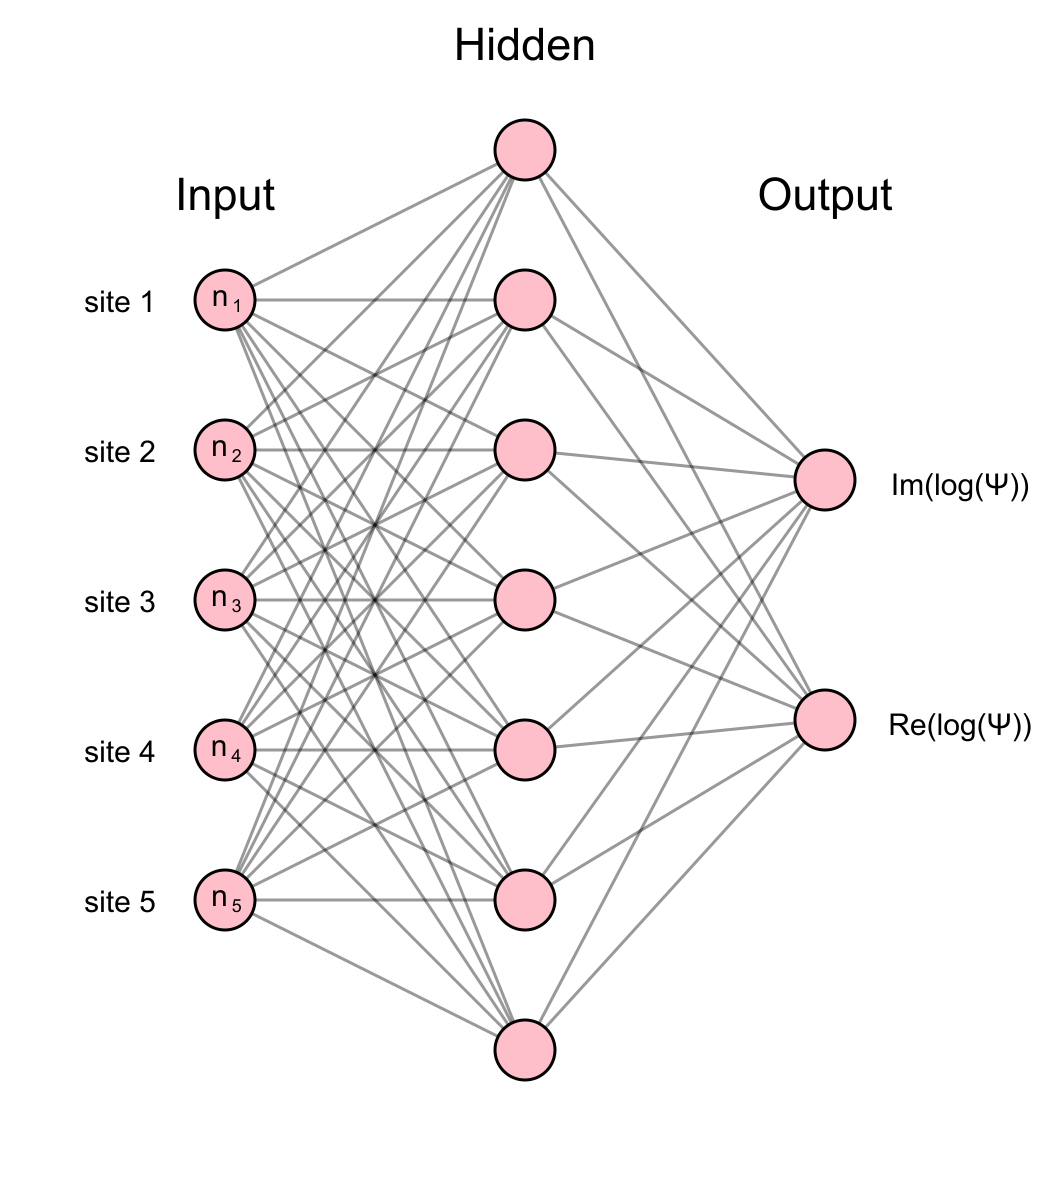
\includegraphics[width=\textwidth]{ch8/ANN.png}
    \end{subfigure}
    \caption{Pictorial representation of the neural network}
    \label{fig:ann}
\end{figure}
%%% FIG %%%
\FloatBarrier \!\!\!\!\!\!\!\!\!\!\!

We take a different approach here by utilizing a universal function approximator instead of any particular form of ansatz. In principle, a feed-forward neural network with sufficient hidden layers and nodes is capable of serving this purpose\cite{lu2020universal} such that the variational parameters are simply the network weights. Let us now consider the wavefunction of the Bose-Hubbard model with $N$ particles and $M$ lattice sites in the occupation basis.

\begin{equation}
    \ket{\Psi} = \sum_{\sum_i n_i = N }\psi(n_1, n_2, ..., n_M)\ket{n_1, n_2, \dots, n_M} = \sum \psi(\mathbf{n})\ket{\textbf{n}}
\end{equation}
The input layer of the network will have $M$ nodes, such that the basis state $\ket{\mathbf{n}} \equiv \ket{n_1, n_2, \dots, n_M}$ can be set as an input as shown in Fig. \ref{fig:ann}. The values of the nodes on the hidden layers are computed as usual, using a hyperbolic tangent activation function:
\begin{equation}
    u_j^{(0)} = n_j \hspace{1cm}; u_m^{(i+1)} = \sum_{k = 1}^{N_H^{(i)}}W_{mk}^{(i+1)}\tanh u_k^{(i)}(\mathbf{n}) + h_m^{(i+1)}
\end{equation}
The output layer will have 2 nodes such that we can get the co-efficient of the input basis state like so:
\begin{equation}
    \psi(\mathbf{n}) = \exp[u_1^{N_l}(\mathbf{n}) + iu_2^{N_l}(\mathbf{n})]
\end{equation}
The wavefunction can now be represented in this compact neural network once we tune the parameters, $\{W^{\mathbf{n}}, h^{\mathbf{n}}\}|_1^{N_l}$ by minimizing the energy. Generally, the expectation value of an operator, $\hat{A}$ is calculated using the expression:
\begin{equation}
    \langle A \rangle = \frac{\sum_{\mathbf{n}, \mathbf{n}'} \psi^*(\mathbf{n})\bra{\mathbf{n}}\hat{A}\ket{\mathbf{n}'}\psi(\mathbf{n}')}{\sum_\mathbf{n} |\psi(\mathbf{n})|^2}
\end{equation}
However, if we compute every element of the sum by retrieving the coefficients from our neural network, we effectively lose the benefit of having a compact representation. Instead, we utilize the standard Monte Carlo scheme, where the basis states are importance sampled, using the Metropolis algorithm. Since our goal is to sample states $\{n\}$ following the distribution $|\psi(\mathbf{n})|^2/\sum_{\mathbf{n}'}|\psi(\mathbf{n}')|^2$, we accept the proposal $\mathbf{n_1} \rightarrow \mathbf{n_2}$ with probability $|\psi(\mathbf{n_2})|^2/|\psi(\mathbf{n_1})|^2$ and compute the expectation value as follows.
\begin{equation}
    \left \langle \bra{\mathbf{n}}\hat{H}\ket{\mathbf{n}} \frac{\psi(\mathbf{n}')}{\psi(\mathbf{n})} \right \rangle_M \equiv \langle H \rangle_M    
\end{equation}
where $\langle\dots\rangle_M$ indicates an average over the metropolis sampling of $\mathbf{n}$. Training the network weights to represent the wavefunction requires us to perform a gradient descent.
\begin{equation}
    w \rightarrow w - \gamma \frac{\partial \langle \hat{H} \rangle_M}{\partial w}
\end{equation}
where, $\gamma$ is the learning rate, and the gradient can be computed using the following expression.
\begin{equation}
    \frac{\partial \langle \hat{H} \rangle}{\partial w} \approx 2\text{Re}(\langle O_w \hat{H}\rangle_M - \langle O_w^*\rangle_M\langle\hat{H}\rangle_M) \hspace{1cm} O_w(\mathbf{n}) = \frac{1}{\psi(\mathbf{n})}\frac{\partial \psi(\mathbf{n})}{\partial w}
\end{equation}
Further details can be found in Saito (2017) \cite{Saito_2017}. Our implementation can be found on \href{https://github.com/20akshay00/MSThesis}{github}, however, in its current state it is unusable due to inefficient computation of the gradient. This leads to extremely large runtimes for even small system sizes. Further, a naive gradient descent approach gets trapped in local minima even for the Bose-Hubbard model\cite{Saito_2017}. As a result, this line of exploration was not pursued further. It is worth noting, however, that there are larger and more mature projects that implement various machine learning techniques to solve many body problems, such as NetKet\cite{Vicentini_2022}.

\section{Stochastic Series Expansion}

We now turn to a class of extremely powerful methods that are broadly classified as Quantum Monte Carlo techniques. There are countless variations and flavors\cite{Pollet_2012, Austin2012} depending on the specifics of the system under consideration, but they all share the trait of utilizing Monte Carlo sampling in some capacity to solve quantum problems. We will focus on one flavor in particular, the stochastic series expansion (SSE)\cite{sandvik2019stochastic}. This section will largely follow the discussion presented in Sandvik's lecture notes\cite{Sandvik_2010}.
\vspace{0.5cm}\\
Generally, the goal of these methods is to compute the partition function and hence the thermal expectation values of various observables of interest. We begin by performing a Taylor expansion of the exponent around $\beta = 0$ and taking the trace with respect to an appropriate basis set $\{\alpha\}$.
\begin{equation}
    Z = \Tr{e^{-\beta H}} = \Tr{\sum_{n = 0}^{\infty} \frac{(-\beta)^n}{n!}H^n} = \sum_{\alpha} \sum_{n = 0}^{\infty} \frac{(-\beta)^n}{n!}\bra{\alpha}H^n\ket{\alpha}
\end{equation}
We can view the above sum as a Monte Carlo sampling of the configurations, $(\ket{\alpha}, n)$ with the weight, $W(\ket{\alpha}, n) = \frac{(-\beta)^n}{n!}\bra{\alpha} H^n \ket{\alpha}$. However, there is a glaring problem, that is the infinite sum over the expansion order, $n$. At first sight, such a situation seems impossible to deal with in a numerical algorithm. However, a solution presents itself if we analyze the nature of the energy and specific heat capacity calculated through this procedure.
\begin{align}\label{eq:mc_energy}
    \langle H \rangle &= \frac{1}{Z}\Tr{He^{-\beta H}} \nonumber\\
    &= \frac{1}{Z}\sum_{\alpha} \sum_{n = 0}^{\infty} \frac{(-\beta)^n}{n!}\bra{\alpha}H^{n+1}\ket{\alpha} \nonumber\\
    &= -\frac{1}{Z}\sum_{\alpha} \sum_{n = 1}^{\infty} \frac{n}{\beta} \cdot \frac{(-\beta)^n}{n!}\bra{\alpha}H^{n}\ket{\alpha} = \frac{\langle n \rangle}{\beta}
\end{align}
Similarly, we get $\langle H^2 \rangle = \langle n(n-1)\rangle/\beta^2$. The expression for the specific heat can then be computed as follows.
\begin{equation}
    C_v = \frac{\langle H^2 \rangle - \langle H \rangle^2}{T^2} = \langle n^2 \rangle - \langle n \rangle^2 - \langle n \rangle
\end{equation}
Generally, the specific heat vanishes as $T \to 0$ for quantum systems, so we can write $\sigma_n = \langle n^2 \rangle - \langle n \rangle^2 = \langle n \rangle$. Thus, we have $\langle n \rangle \sim N\beta$ and $\sigma_n \sim \sqrt{N\beta}$ where $N$ is the system size which is introduced since the energy roughly scales with the $N$. This tells us that the distribution of $n$ that contributes to the sum is quite narrow and we can simply introduce a cut-off length $L$ in our algorithm (that must be adjusted as the simulation progresses). 

%%% FIG %%%
\begin{figure}[!htb]
    \centering
    \begin{subfigure}[b]{0.75\textwidth}  %keep total sum <1 to show in same line
        \centering
        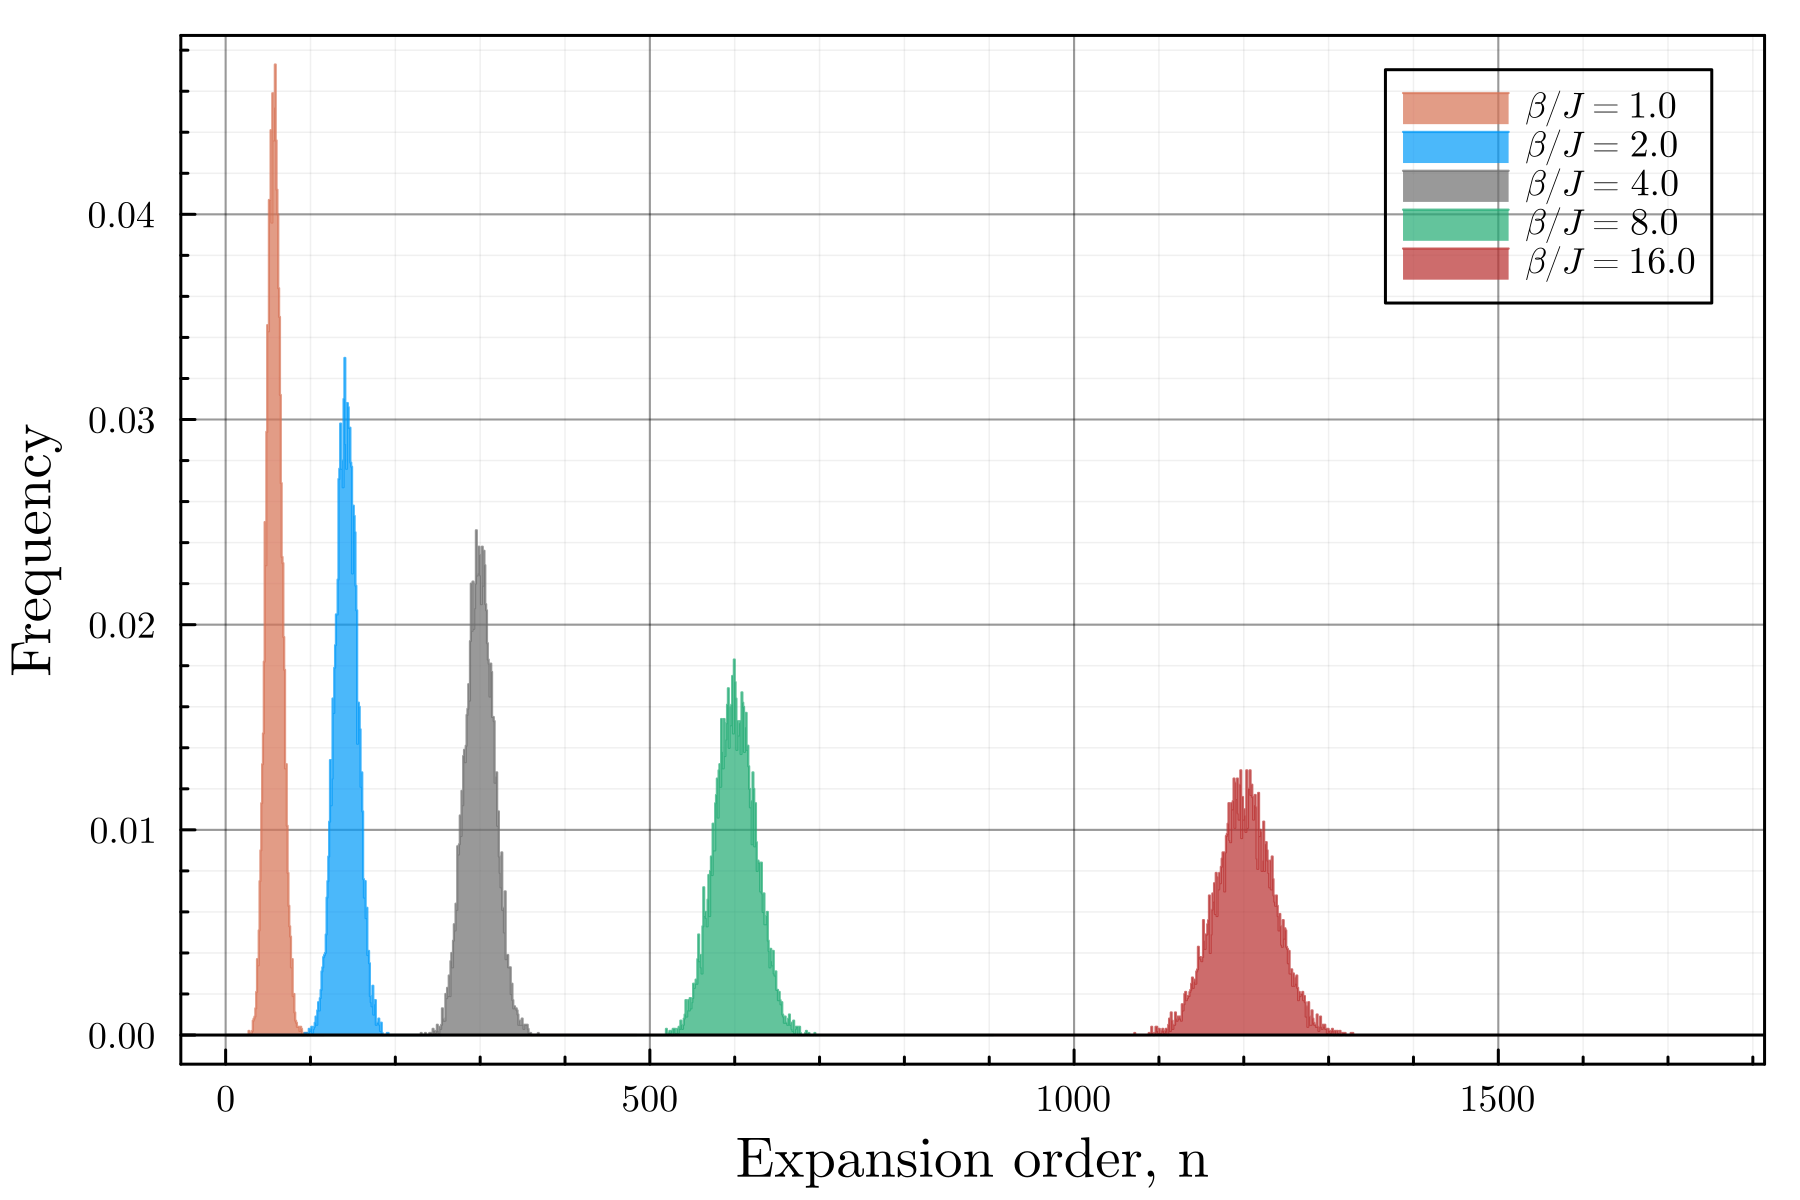
\includegraphics[width=\textwidth]{ch8/ndist.png}
    \end{subfigure}
    \caption{Distribution of expansion order in SSE}
    \label{}
\end{figure}
%%% FIG %%%
\FloatBarrier \!\!\!\!\!\!\!\!\!\!\!

\vspace{-0.5cm}
At this point, we note that computing the quantity $\bra{\alpha}H\ket{\alpha}$ is generally non trivial, and so we introduce an important idea that makes the SSE tractable. Generally, lattice Hamiltonians can be broken down as $H = -\sum_{a, b} H_{a, b}$, where $b$ indicates the "bond" connecting two sites $i(b)$ and $j(b)$, and $a$ indicates the class of the operator. Any power of the Hamiltonian can then be written in terms of a sum over 'operator strings' $\{H_{ab}\}$.
\begin{equation}
    (-H)^n = \sum_{\{H_{ab}\}} \prod_{p = 1}^n H_{a(p), b(p)}
\end{equation}
Putting this together with the fixed length scheme that was motivated above, we can write the partition function in the typical monte carlo format.
\begin{equation}
    Z = \sum_{\alpha, H_{ab}} \frac{\beta^n (L - n)!}{L!} \bra{\alpha}\prod_{p = 1}^n H_{a(p), b(p)}\ket{\alpha} \hspace{0.5cm} \leftrightarrow \hspace{0.5cm} Z = \sum_{C_i} W(C_i)    
\end{equation}

\begin{equation}
    \langle O \rangle = \frac{1}{Z}\sum_{\alpha, H_{ab}} \frac{\beta^n (L - n)!}{L!} \bra{\alpha}O\prod_{p = 1}^n H_{a(p), b(p)}\ket{\alpha} \hspace{0.5cm} \leftrightarrow \hspace{0.5cm} \langle A \rangle = \frac{\sum_{C_i} O(C_i)W(C_i)}{\sum_{C_i} W(C_i)}
\end{equation}
We have now introduced an abstract configuration which is a 2-tuple consisting of $\ket{\alpha}$, an element of the basis set, and $\{H_{ab}\}$ which is a string of $L$ bond operators. In order to work with the fixed-length scheme, we have also introduced $H_{0,0} = \mathbb{I}$ to pad the operator string, such that each string consists of $n$ non-identity bond operators and $(L-n)$ identities, thus sampling the expansion orders $n \in [1, L]$. 
\vspace{0.5cm}\\
The problem has now reduced to ergodically sampling this configuration space according to their weights (which can be computed with ease due to the bond decomposition). An issue arises when the weights are not positive, in which case they cannot be interpreted as probabilities, thus giving rise to the infamous \textit{sign problem}\cite{pan2022sign}. This is usually the case for fermionic systems and systems with non-bipartite lattices geometries. 

\subsection{S=1/2 Heisenberg model}
Let us now consider the spin-1/2 Heisenberg model with anti-ferromagnetic interactions ($J > 0$) on a square lattice. We choose this particular example since it is quite illustrative of the SSE technique while also having some relevance to the Bose-Hubbard model that we will discuss at the end of the chapter.  
\begin{equation}
    H = J\sum_{\langle i, j \rangle} S_i \cdot S_j
\end{equation}
A natural basis set to use in our expansion is the $S_z$-basis, $\ket{S_1^z, S_2^z, \cdots, S_N^z}$. We can now rewrite the Hamiltonian as a sum of bond operators:
\begin{equation}
    H_{1, b} = \frac{1}{4} - S_{i(b)}^z S_{j(b)}^z \hspace{1cm} H_{2, b} = \frac{1}{2}(S_{i(b)}^+ S_{j(b)}^- + S_{i(b)}^- S_{j(b)}^+)    
\end{equation}
\begin{equation}
    H = J\sum_{b = 1}^B [S_{i(b)}^z S_{j(b)}^z + \frac{1}{2}(S_{i(b)}^+ S_{j(b)}^- + S_{i(b)}^- S_{j(b)}^+)] = -J\sum_{b=1}^{N_B}(H_{1, b} - H_{2, b}) + \frac{JN_b}{4}
\end{equation}
Here, we have introduced two 'classes' of bond operators, that is, those that are diagonal ($H_{1, b}$) and off-diagonal ($H_{2, b}$) in the $S_z$-basis.
There is also an important restriction on the choice of the bond operators $H_{a,b}$, namely, that they must be non-branching, i.e, $H_{a,b}\ket{\alpha_i} = C_{a,b}^{i, j} \ket{\alpha_j}$ where $\ket{\alpha_i}$ and  $\ket{\alpha_j}$ are single elements of the chosen basis set. This implies that each configuration can equivalently be understood as a periodic sequence of basis elements (due to the cyclic nature of the trace).
\begin{equation}
    C \equiv \ket{\alpha_0} \rightarrow \ket{\alpha_1} \rightarrow \dots \rightarrow \ket{\alpha_{L-1}} \rightarrow \ket{\alpha_0} \hspace{1cm} \ket{\alpha_i} = \prod_{p=1}^iH_{a(p), b(p)}\ket{\alpha_0}
\end{equation}
Notice that we have also introduced a constant energy shift in order to force the matrix elements, and hence the configuration weights to be positive. Since the bond operators only act on two sites, we can list out all of these matrix elements:
\begin{align*}
    &\bra{\uparrow_{i(b)} \downarrow_{j(b)}}H_{1, b}\ket{\uparrow_{i(b)} \downarrow_{j(b)}} = \frac{1}{2}\hspace{1cm} \bra{\downarrow_{i(b)} \uparrow_{j(b)}}H_{2, b}\ket{\uparrow_{i(b)} \downarrow_{j(b)}} = \frac{1}{2} \\ 
    &\bra{\downarrow_{i(b)} \uparrow_{j(b)}}H_{1, b}\ket{\downarrow_{i(b)} \uparrow_{j(b)}} = \frac{1}{2} \hspace{1cm}     \bra{\uparrow_{i(b)} \downarrow_{j(b)}}H_{2, b}\ket{\downarrow_{i(b)} \uparrow_{j(b)}} = \frac{1}{2} 
\end{align*}
Note that any bond operator can only act on anti-parallel spins, since all other configurations have a vanishing matrix element. Further, we see that not only are the non-zero matrix elements positive but they are also equal. This greatly simplifies the algorithm, since the weight of any valid configuration is simply computed as follows.
\begin{equation}
    W(\alpha, \{H_{a, b}\}) = \left ( \frac{\beta}{2} \right )^n \frac{(L - n)!}{L!}
\end{equation}
The challenge now is to come up with a sampling scheme that generates operator strings that samples such periodic sequences of basis elements. There are usually three types of updates that are required to maintain ergodicity:
\begin{itemize}
    \item \textbf{Diagonal update:} This changes $n$, the number of non-identity bond operators in the operator string. Such an update simply replaces an identity operator with a diagonal one  (or vice versa) if the spin states it acts on is anti-parallel. 
    \item \textbf{Off-diagonal update: } Off-diagonal operators cannot be added or removed individually as was the case with the diagonal operators, since the periodicity of the basis state has to be preserved. As a result, one has to manipulate pairs of off-diagonal operators acting on the same sites, however such an update scheme is quite inefficient. Instead, another approach known as the operator loop update\cite{Sandvik_1999} is used wherein a loop is constructed across the entire configuration, connecting the spin sites at the base of several operators, which are then flipped simultaneously in an analogous manner to the cluster updates in the Ising model. This scheme is related to a broader class of loop algorithms\cite{evertz2003} applicable to general quantum monte carlo methods.
    \item \textbf{Spin-flip update: } Finally, if a particular spin is not acted upon by any operators, it can be flipped to sample a different basis state $\ket{\alpha}$. However, this update is not strictly required nor efficient since the off-diagonal updates already sample the basis states as well.
\end{itemize}

The probability of accepting these updates can then be computed by means of the usual constraint arising from detailed balance of the markov chain of configurations.
\begin{equation}
    P_{\text{accept}}(A \to B) = \min \left (\frac{W(B)P_{\text{select}}(B \to A)}{W(A)P_{\text{select}}(A \to B)}, 1\right )
\end{equation}
The interested reader may find the details of the sampling scheme as well as an ingenious way to visualize and implement the SSE in Sandvik's lecture notes\cite{Sandvik_2010}. 
\vspace{0.5cm}\\
Once we are able to sample the configurations ergodically, diagonal observables can be computed easily as they do not alter the sequence of basis states. On the other hand, off-diagonal observables are quite hard to compute, in general. However, any off-diagonal operator, $H_{2, b}$, which is a part of the Hamiltonian is found to be related to the expectation value of the number of occurences of the operator in the operator string\cite{Sandvik_2010}. For example, this is what we found for the energy in Eq. \eqref{eq:mc_energy}. Luckily, most of the observables that are required for our purposes fall within these two categories.

\subsection{Results}
We have performed the SSE for various lattice sizes and temperatures, recording $n=10000$ samples for computing each quantity. The results are shown as in Fig. \ref{fig:sse_res}. Although there are strong finite-size effects in most of the plots, we can see for $L=48$ that the (staggered) magnetization seems to undergo a transition somewhere between $J \cdot T \in [0.2, 0.6]$ indicating a shift from an anti-ferromagnet to a paramagnet. Peculiarly, the magnetic susceptibility $\chi$ seems to also have a continuous transition around the same region instead of a divergence as expected from a second order transition. On the other hand, we have some hint of divergence from the specific heat plot around $J\cdot T \approx 0.6$. 

%%% FIG %%%
\begin{figure}[!htb]
    \centering
    \begin{subfigure}[b]{\textwidth}  %keep total sum <1 to show in same line
        \centering
        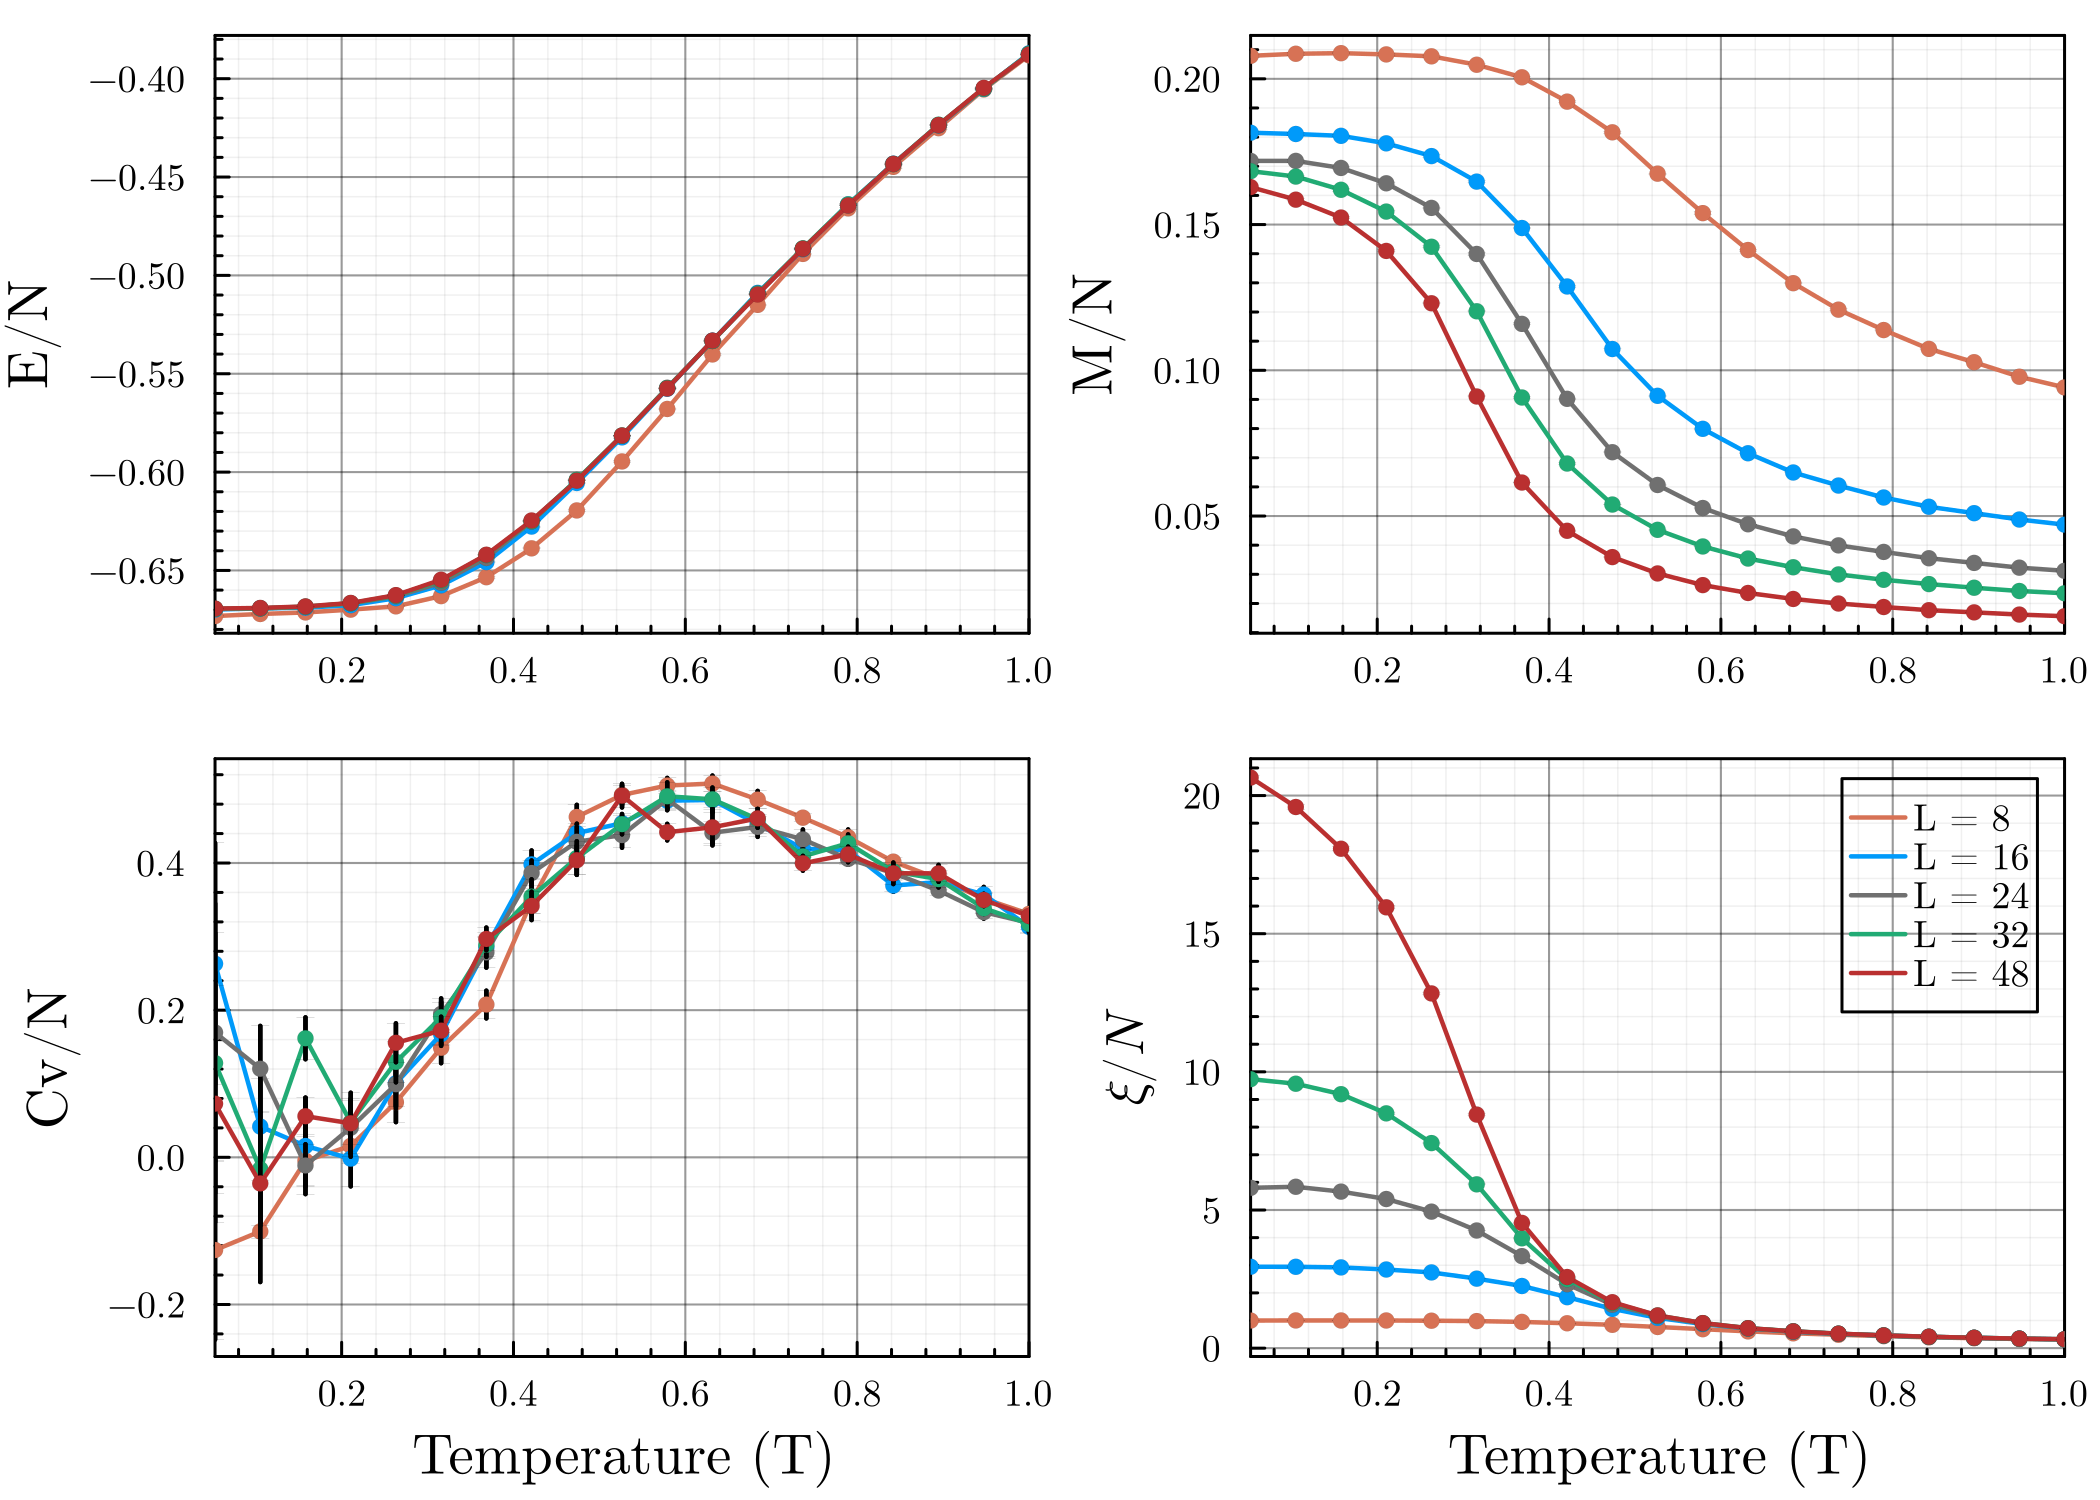
\includegraphics[width=\textwidth]{ch8/sse_stats.png}
    \end{subfigure}
    \caption{Tracking various quantities calculated using SSE}
    \label{fig:sse_res}
\end{figure}
%%% FIG %%%
\FloatBarrier \!\!\!\!\!\!\!\!\!\!\!

In order to extract a better estimate of the critical temperature by dealing with the finite size effects, we calculate the Binder cumulant for various lattice sizes in Fig. \ref{fig:sse_bc}. 
\begin{equation}
    U_L = 1 - \frac{\langle M^4 \rangle_L}{3\langle M^2 \rangle^2_L}
\end{equation}

%%% FIG %%%
\begin{figure}[!htb]
    \centering
    \begin{subfigure}[b]{\textwidth}  %keep total sum <1 to show in same line
        \centering
        \includegraphics[width=0.75\textwidth]{ch8/sse_binder.png}
    \end{subfigure}
    \caption{Binder cumulant curves for various lattice sizes}
    \label{fig:sse_bc}
\end{figure}
%%% FIG %%%
\FloatBarrier \!\!\!\!\!\!\!\!\!\!\!

\vspace{-0.3cm}
We see that the curves roughly intersect at $J\cdot T \approx 0.22$. As it stands, these results significantly contradict with each other and we have not been able to resolve this so far. 

\subsection{Mapping to bosons}
The discussion so far seems rather unrelated to the rest of the thesis, however, a closer look at the Heisenberg Hamiltonian reveals that this is not the case:
\begin{equation}
    H = J\sum_{\langle i, j \rangle} \vec{S}_i \cdot \vec{S}_j = J\sum_{\langle i, j \rangle} \left [\frac{1}{2}(S_i^+ S_j^- + S_i^- S_j^+) +  S_i^z S_j^z \right ]
\end{equation}
Consider the mapping $S^+_i \to a_i^{\dagger}$, $S_i^- \to a_i$ and $S^z_i = n_i - 1/2$. The Hamiltonian is then oddly reminiscent of the extended Bose-Hubbard model.
\begin{equation}
    H = \frac{J}{2} \sum_{\langle i, j \rangle}(a_i^{\dagger}a_j + a_j^{\dagger}a_i) + J \sum_{\langle i, j \rangle} n_i n_j
\end{equation}
where $t = -J/2$ and $V = J$. Note that the on-site interaction term is missing. This is because we have effectively mapped classical spin-1/2 particles to hardcore bosons, i.e, in the limit of $U \to \infty$ s.t. $\langle n_i \rangle \in \{0, 1\}$. Loosely we can think of states having $\langle S^z \rangle = -1/2$ and $\langle S^z \rangle = 1/2$ corresponding to $\langle n \rangle = 0$ and $\langle n \rangle = 1$ boson occupation, respectively. Note that the $a^{\dagger}$ ($a$) operators here are not general bosonic operators, but specifically ones that create (annihilate) hard-core bosons.

%%% FIG %%%
\begin{figure}[!htb]
    \centering
    \begin{subfigure}[b]{\textwidth}  %keep total sum <1 to show in same line
        \centering
        \includegraphics[width=\textwidth]{ch8/bosonspin.png}
    \end{subfigure}
    \caption{Mapping hard-core bosons to classical spin-1/2 particles}
    \label{}
\end{figure}
%%% FIG %%%
\FloatBarrier \!\!\!\!\!\!\!\!\!\!\!

In the most general case, we can map a spin-S anisotropic XXZ model to a semi-hardcore extended Bose-Hubbard model with maximum occupation of $2S$.

\begin{minipage}{0.7\textwidth}
\begin{align*}
    H &= J_x\sum_{\langle i, j \rangle} (S_i^+ S_j^- + S_i^- S_j^+) +  J_z\sum_{\langle i, j \rangle} S_i^z S_j^z + h_z \sum_i S_i^z\\
    H &= -t \sum_{\langle i, j \rangle}(a_i^{\dagger}a_j + a_j^{\dagger}a_i) + V \sum_{\langle i, j \rangle} n_i n_j - \mu \sum_i n_i
\end{align*}    
\end{minipage}
\begin{minipage}{0.25\textwidth}
    \begin{align*}
        t &\equiv J_x \\
        V &\equiv J_z \\ 
        \mu &\equiv J_z - h_z
    \end{align*}
\end{minipage}

However, in such a case, there are many more non-zero matrix elements that exist which are also not necessarily equal in magnitude. As a result, the operator loop update has to be redesigned since there is no unique deterministic loop that can be constructed for a given configuration. This can be remedied by utilizing the directed loop algorithm\cite{Syljusen_2002} which applies to the most general situations. 
\vspace{0.5cm}\\
Our implementation of the SSE for the isotropic spin-1/2 Heisenberg model can be found on \href{https://github.com/20akshay00/MSThesis}{github}. Although we intended to implement the directed loop algorithm as well, we were unable to do so within the constraint of the thesis and will not discuss its details here. 

\section{World-line QMC}
While the SSE is quite straightforward conceptually, it can efficiently generate samples only when the diagonal and off-diagonal terms are of comparable magnitude\cite{Sandvik_2010} ($t \sim U, t \sim V$ for e.g.). This is generally satisfied for spin systems, however, the interesting regions in bosonic systems occur for $t \ll U, t \ll V$. As a result, the SSE sampling scheme is not the best choice for our purposes. Instead, we turn to a related class of algorithms loosely termed as world-line QMC\cite{schneider2008}. We first discuss the discrete formulation.
\begin{equation}
    Z = \Tr{e^{-\beta H}}  = \Tr{\prod_{l = 1}^L e^{-\Delta\tau H}} \hspace{1cm} \Delta \tau = \beta/L
\end{equation}
Instead of expanding the exponential as a Taylor series, we utilize a Trotter decomposition to cast the sum in terms of the usual monte carlo language by inserting completeness relations of our prefered basis set, $\{\alpha \}$. We then have:
\begin{equation}
    Z = \sum_{\alpha_0}\sum_{\alpha_1}\dots\sum_{\alpha_L - 1} \bra{\alpha_0}e^{-\Delta\tau H}\ket{\alpha_{L-1}}\dots \bra{\alpha_2}e^{-\Delta\tau H}\ket{\alpha_1}\bra{\alpha_1}e^{-\Delta\tau H}\ket{\alpha_0}
\end{equation}
\begin{equation}
    Z \approx \sum_{\{\alpha\}}\bra{\alpha_0}1 - \Delta \tau H \ket{\alpha_{L-1}}\dots \bra{\alpha_2}1 - \Delta \tau H \ket{\alpha_1}\bra{\alpha_1}1 - \Delta \tau H \ket{\alpha_0}
\end{equation}
where, the error falls of as $\mathcal{O}(\Delta \tau)$ and vanishes in the limit $\Delta\tau \to 0$. The configurations here are quite similar to the idea we introduced in the SSE involving a cyclic sequence of basis states. While the diagonal parts of $H$ leave the basis state unaltered, the off-diagonal ones do not. Effectively, we can view this procedure as having introduced a new dimension, $\Delta \tau$ to our system. 
\vspace{0.5cm}\\
In principle, since the results of the above method are only exact when $\Delta \tau \to 0$, we must perform the simulation for various values of $\Delta \tau$ and extrapolate them to get the exact results. However, it turns out that such a technique is unnecessary as we can, infact, take the limit exactly to formulate a continuous time world-line approach\cite{schneider2008}. 
\begin{equation}
    Z = \Tr{e^{-\beta H}} = \Tr{\mathcal{T} e^{\beta H_0} \exp{-\int_0^{\beta} d\tau V(\tau)}}
\end{equation}
where, $V(\tau) = e^{\tau H_0}Ve^{-\tau H_0}$. The exponential can be expanded iteratively like so:
\begin{equation}
    Z = \Tr{e^{-\beta H_0} \sum_{n = 0}^{\infty} \int_0^{\beta} d\tau_1 \int_0^{\tau_1}d\tau_2\dots\int_0^{\tau_{n-1}} V(\tau_1)\dots V(\tau_n)}
\end{equation}
By inserting basis sets between the elements, this formulation becomes quite similar to the discrete case, except that the $d\tau$ dimension is now continuous. However, a naive sampling of these configurations would result in critical slowing down near the phase boundaries (among other issues)\cite{Prokofev1998}. There exists an analog of the directed loop updates for the continuous-time world-line approach, called the worm algorithm\cite{prokofev2010worm, Pollet_2007, sadoune2022efficient} which solves this issue. We intend to utilize this technique in our future studies to obtain more quantitative results.


% Choosing a relevant basis set $\{\ket{\alpha_i}\}$, we can then insert completeness relations to break down the expression for the partition function. 
% $$Z = \sum_{n=0}^{\infty} \frac{(-\beta)^n}{n!}\sum_{\{\alpha\}_n} \bra{\alpha_0}H\ket{\alpha_{n-1}}\dots\bra{\alpha_2}H\ket{\alpha_1}\bra{\alpha_1}H\ket{\alpha_0}$$

% The expectation value of the Hamiltonian can then be written like so:
% \begin{align*}
%     E &= \langle H \rangle = \frac{1}{Z}\Tr{He^{-\beta H}}\\
%      &= \frac{1}{Z}\sum_{n=0}^{\infty} \frac{(-\beta)^n}{n!}\sum_{\{\alpha\}_{n+1}} \bra{\alpha_0}H\ket{\alpha_{n+1}}\dots\bra{\alpha_2}H\ket{\alpha_1}\bra{\alpha_1}H\ket{\alpha_0}    \\
%      &= -\frac{1}{Z}\sum_{n=1}^{\infty} \frac{(-\beta)^n}{n!} \cdot \frac{n}{\beta} \cdot \sum_{\{\alpha\}_n} \bra{\alpha_0}H\ket{\alpha_n}\dots\bra{\alpha_2}H\ket{\alpha_1}\bra{\alpha_1}H\ket{\alpha_0}  = \frac{\langle n \rangle}{\beta}   
% \end{align*}

\chapter{Summary \& Future prospects}\label{ch8}
We started by setting up the formalism to describe the physics of interacting bosons in a periodic lattice. We then proceeded to generate the ground state phase diagram for bosons with contact interactions and successfully extracted the phase boundary for the Mott insulator to superfluid transition. This was done numerically using Mean-field and Cluster Mean-field techniques.
\vspace{0.5cm}\\
Upon deeming the latter to be impractical for our requirements, we moved on to study the ground state phases exhibited in the presence of long-range interactions at a mean-field level. As a result, we observed extended regions of two new phases, density waves and supersolids for any non-zero magnitude of the strength of nearest-neighbour interactions. We then introduced a spin-degree of freedom and analyzed its effect on the nature of the Mott insulator to superfluid transition. This directly led to a simple analysis of the phenomenon of mediation through bosons to induce effective interactions between non-interacting particles.
\vspace{0.5cm}\\
Finally, we presented a brief review of Variational QMC and Stochastic Series Expansion to study the Bose-Hubbard model beyond the mean-field level. While the basic framework was implemented and initial results were obtained, this line of work is still at an early stage and did not generate tangible insight. In the future, we plan to corroborate and extend the results obtained in this thesis using the state-of-the-art worm algorithm to study the finite temperature physics of the Bose-Hubbard model.



\fancyhead[L]{\appendixname\ \thechapter\ --\ \leftmark}

\begin{appendices}
\chapter{Implementation details}
\section{Exact Diagonalization}\label{sec:ed_imp}
The details to implement exact diagonalization for the canonical ensemble (CE) is described in great detail in Zhang et. al. (2010)\cite{Zhang_2010}. We will instead discuss a scheme to extend it to the grand canonical ensemble (GCE) as is required to implement the cluster mean field approximation.
\vspace{0.5cm}\\
Once we have written a function to compute the Hamiltonian $H(N, L)$ for a system of $N$ bosons on $L$ lattice sites, the GCE Hamiltonian is simply given by the direct sum $H_{\text{GCE}} = \oplus_{N = 1}^{\infty} H(N, L)$. For numerical feasibility, we will set an upper bound on the particle number, $N \leq N_{max}$. This effectively means that $H_{GCE}$ can be constructed as a block diagonal matrix using the set of CE Hamiltonians, $\{H(N, L)\}|_{N=1}^{N_{max}}$, since $\hat{H}_{BHM}$ commutes with $\hat{N} = \sum_{i} \hat{n}_i$. While the scheme outlined above is perfectly valid, we will also describe a different approach due to its similarity with the implementation rrquired for the mean-field approximation. 
\vspace{0.5cm}\\
Consider the local annihilation operator, $\tilde a_i$, on a particlar site $i$. Given a maximum particle occupation of $N_{max}$, we can write the operator in the local occupation basis $\{n_i\}$ as a sparse matrix with $\{ \sqrt{1}, \sqrt{2}, \dots, \sqrt{N_{max}}\}$ as the lower off-diagonal. We can then construct $\tilde a_i^{\dagger}$ as the conjugate transpose and $\tilde n_i$ as $\tilde a_i^{\dagger} \tilde a_i$. Note that the bosonic commutation relations imply a tensor product structure for the combined space of multiple bosonic particles (which is not the case for fermions). As a result, we can construct the global/lattice operators, $O_i$ using the local operators $\tilde O_i$ as follows.
\begin{equation}
    O_i = \underbrace{\mathbb{I} \otimes \dots \otimes \mathbb{I}}_{(i-1)\text{ times}} \otimes \tilde O_i \otimes \underbrace{\mathbb{I} \otimes \dots \otimes \mathbb{I}}_{(L - i) \text{ times}} 
\end{equation}
The GCE Hamiltonian can then be easily constructed using the constituent lattice operators $a_i$, $a_i^{\dagger}$ and $n_i$. 
\vspace{0.5cm}\\
A closer look reveals that the two schemes differ only in the choice of basis that we have utilized to construct the Hamiltonian. The first case uses a direct sum of basis sets of each fixed particle number subspace, $\ket{\Psi} = \oplus_{N=1}^{N_{max}}\ket{\Psi(N, L)}$, whereas the second case uses a tensor product of the local occupation basis, $\ket{\Psi'} = \otimes_{k=1}^{L}\ket{\Psi'(N_{max}, k)}$.

\section{Mean field theory}

\subsection{Bose Hubbard model}
In this case, we simply have to construct the single-site Hamiltonian in Eq. \eqref{eq:bhm_mft} given a maximum particle occupation of $N_{max}$. Since we are forced to work with the GCE within this mean-field decoupling, we note that we have already constructed the required local site operators as discussed in Sec. \ref{sec:ed_imp}. The local Hamiltonian is then easily constructed and the mean-field parameter is determined self-consistently using fixed point iteration. A combination of absolute and relative tolerances are used to set the convergence limit for the self-consistency loop, i.e, the condition is as follows; $(x^{(n + 1)} - x^{(n)})  \leq \epsilon_{\text{atol}} + \epsilon_{\text{rtol}} * x^{(n)}$. 

\subsection{Extended Bose Hubbard model}
In this case, we have to construct the Hamiltonian over a unit cell of lattice sites as shown in Eq. \eqref{eq:ebhm_mft}. The unit cell operators can be constructed using the tensor product structure discussed in Sec. \ref{sec:ed_imp} except that we use the number of sites in the unit cell, $L_{UC}$, instead of the total number of lattice sites, $L$. The Hamiltonian can then be constructed for an arbitrary unit cell by taking the connectivity matrix as an input and using the relation in Eq. \eqref{eq:unit_cell} to build the mean-field decoupled terms. The non-linearity introduced by the unit cell structure result in convergence issues during the self-consistency procedure. This has been discussed in depth in Sec. \ref{sec:caveats}.

\subsection{Spin-1 Bose Hubbard model}
This case is quite similar to the Bose Hubbard model, however, we must construct three kinds of creation/annihilation operators corresponding to each spin projection, $\sigma \in \{1, 0, \overline{1}\}$. Note that we have an important constraint to consider, namely, that $\sum_{\sigma} n_{i\sigma} \leq N_{max}$ on each lattice site. This can be enforced by enumerating the Fock-space basis set for a lattice with 3 sites and $N$ bosons such that $N \leq N_{max}$. The procedure is the same as the one used in constructing the CE Hamiltonian for exact diagonalization in Sec. \ref{sec:ed_imp}.
\vspace{0.5cm}\\
While it is tempting instead to utilize a tensor product structure as in the previous section, it becomes cumbersome since we require $\sum_{\sigma} n_{i\sigma} \leq N_{max}$ instead of the naturally imposed condition, $n_{i\sigma} \leq N_{max}$. The second case would effectively result in a maximum site occupation of $3N_{max}$, however, it only takes into account the lower energy states since each spin state occupation cannot exceed $N_{max}$. As a result, the tensor product technique would not enumerate the entire basis set consistently. Surprisingly, the phase boundary predicted by this method still matches the true result, although the nature of the phases are altered (for e.g. the net spin in Mott insulator lobes are capped at $N_{max}$ instead of $3N_{max}$).

\section{Code repository}

All code used in this project was written in \href{https://julialang.org/}{Julia 1.8}\cite{Julia-2017} and can be found at \url{https://github.com/20akshay00/MSThesis}. All figures and diagrams were generated using \href{https://github.com/JuliaPlots/Plots.jl}{Plots.jl}\cite{christ2022plotsjl} and \href{https://github.com/JuliaGraphics/Luxor.jl}{Luxor.jl}. The following packages were utilized in varying capacities for implementing the numerical techniques: \href{https://github.com/JuliaNLSolvers/Optim.jl}{Optim.jl}\cite{mogensen2018optim}, \href{https://github.com/francescoalemanno/FixedPoint.jl}{FixedPoint.jl} and \href{https://github.com/Jutho/KrylovKit.jl}{KrylovKit.jl}. 
\chapter{Diagonalizing spin interactions}\label{app:rotation}
Consider the following hamiltonian for a spin-1/2 particle.

\begin{equation}\label{eq:spin-half}
    H = \vec{S} \cdot \vec{\sigma} = \begin{pmatrix}
        \cos\theta & \sin\theta e^{i\phi} \\ 
        \sin\theta e^{i\phi} & -\cos\theta    
    \end{pmatrix}
\end{equation}

where $S \equiv (\cos\phi\sin\theta, \sin\phi\sin\theta, \cos\theta)$ is a classical spin with $|S| = 1$. 
\vspace{0.5cm}\\
It is easily seen that the hamiltonian can be diagonalized by the following unitary matrix.
\begin{equation}\label{eq:rot}
    U = \begin{pmatrix}
        \cos\frac{\theta}{2} & -\sin\frac{\theta}{2}e^{-i\phi} \\ 
        \sin\frac{\theta}{2}e^{i\phi} & \cos\frac{\theta}{2}
    \end{pmatrix}
\end{equation}
Generally such a matrix is only unique upto a permutation and scaling of the columns. We would like to find a simple scheme to find such a matrix for systems with spin $>$ 1/2 without having to compute the eigenvectors first. Thinking about this procedure from a different perspective, we simply want to find a matrix that rotates the spin quantization axis from $\hat{z}$ to align with $\vec{S}$.

%%% FIG %%%
\begin{figure}[!htb]
    \centering
    \begin{subfigure}[b]{\textwidth}  %keep total sum <1 to show in same line
        \centering
        \includegraphics[width=0.5\textwidth]{appendix/rotation.png}
    \end{subfigure}
    \caption{Rotating the quantization axis}
\end{figure}
%%% FIG %%%
\FloatBarrier \!\!\!\!\!\!\!\!\!\!\!

This can be achieved by rotating the system by an angle of $\theta$ about the axis $\hat{n} = \hat{z} \cross \vec{S} =  (-\sin\phi, \cos\phi, 0)$. For a spin-1/2 particle, the rotation matrix is given as follows.
\begin{equation}
    R_{\vec{n}}(\alpha) = \exp{-\frac{\alpha}{2}\vec{n}\cdot\vec{\sigma}} = \mathbb{I}\cos\frac{\alpha}{2} + i (\hat{n}\cdot \vec{\sigma})\sin\frac{\alpha}{2}
\end{equation}
For our choice of rotation axis, this gives us the following matrix which is exactly what we found earlier in Eq. \eqref{eq:rot}!
\begin{equation}
    U = \begin{pmatrix}
        \cos\frac{\alpha}{2} + in_z\sin\frac{\alpha}{2} & i\sin\frac{\alpha}{2}(n_x - in_y) \\ 
        i\sin\frac{\alpha}{2}(n_x + in_y) & \cos\frac{\alpha}{2} - in_z\sin\frac{\alpha}{2}
    \end{pmatrix} =
    \begin{pmatrix}
        \cos\frac{\theta}{2} & -\sin\frac{\theta}{2}e^{-i\phi} \\ 
        \sin\frac{\theta}{2}e^{i\phi} & \cos\frac{\theta}{2}
    \end{pmatrix}
\end{equation}

Similarly, let us now consider the same hamiltonian in Eq. \ref{eq:spin-half} for a spin-1 particle.

\begin{equation}\label{eq:spin-one}
    H = \vec{S} \cdot \vec{J} = \begin{pmatrix}
        \cos\theta & \frac{1}{\sqrt{2}}\sin\theta e^{-i\phi} & 0 \\
        \frac{1}{\sqrt{2}}\sin\theta e^{i\phi} & 0 & \frac{1}{\sqrt{2}}\sin\theta e^{-i\phi} \\ 
        0 & \frac{1}{\sqrt{2}}\sin\theta e^{i\phi} & -\cos\theta
    \end{pmatrix}
\end{equation}

where $\vec{J}$ are the spin-1 matrices. The rotation matrix can then be written as follows\cite{Curtright_2014}.
\begin{equation}
    R_{\vec{n}}(\alpha) = \exp{-i\alpha \hat{n}\cdot\vec{J}} = \mathbb{I} + i\hat{n}\cdot\vec{J}\sin\alpha + (\hat{n}\cdot\vec{J})^2 (\cos\alpha - 1)
\end{equation}
Expanding this for our choice of rotation angle and axis, we obtain:
\begin{equation}
    U = \begin{pmatrix}
        \cos^2\frac{\theta}{2} & -\frac{1}{\sqrt{2}}\sin\theta e^{-i\phi} & \sin^2\frac{\theta}{2} e^{-2i\phi} \\
        \frac{1}{\sqrt{2}}\sin\theta e^{i\phi} & \cos\theta &-\frac{1}{\sqrt{2}}\sin\theta e^{-i\phi}\\
        \sin^2\frac{\theta}{2}e^{2i\phi} & \frac{1}{\sqrt{2}}\sin\theta e^{i\phi} & \cos^2\frac{\theta}{2}
    \end{pmatrix}
\end{equation}

It can be easily checked that this matrix does indeed diagonalize the hamiltonian in Eq. \eqref{eq:spin-one}. Thus, in general, such a hamiltonian is diagonalized by the rotation matrix that aligns the quantization axis to $\vec{S}$. This nice structure emerges due to the relation between the group that governs spin transformations, $SU(2)$, and the group that governs rotations in euclidean space, $SO(3)$\cite{palash2019}.
\chapter{Computing vacuum expectations}\label{app:wick}
Consider the following situation. We have a degenerate subspace of doubly-occupied ground states and a perturbative hamiltonian, $V = \sum_{ii'\sigma\sigma'} g^{\sigma\sigma'}_{ii'} (d_{i\sigma}^{\dagger}d_{i'\sigma'} + h.c.)$. We are now required to compute matrix elements as follows.

\begin{equation}
    \bra{\phi}V\ket{\psi} = \sum_{\substack{ii'\\ \sigma\sigma'}} g^{\sigma\sigma'}_{ii'} \bra{0}d_{m'\beta'}d_{m\beta}d_{i\sigma}^{\dagger}d_{i'\sigma'}d_{l\alpha}^{\dagger}d_{l'\alpha'}^{\dagger}\ket{0}
\end{equation}
where $\ket{\psi} \equiv d_{l\alpha}^{\dagger}d_{l'\alpha'}^{\dagger}\ket{0}$ and $\ket{\phi} \equiv d_{m\beta}^{\dagger}d_{m'\beta'}^{\dagger}\ket{0}$. Such a general vacuum expectation can be resolved using the rules of Wick contractions\cite{Kvaal15} as shown below.

\begin{equation}
\wick{
\c1 d_{m'\beta'} 
\c2 d_{m\beta} 
\c1 d_{i\sigma}^{\dagger} 
\c3 d_{i'\sigma'} 
\c2 d_{l\alpha}^{\dagger}  
\c3 d_{l'\alpha'}^{\dagger} 
}
\hspace{0.5cm}
\longrightarrow
\hspace{0.5cm}
\delta_{m'i}
\delta_{\beta'\alpha}
\delta_{ml}
\delta_{\beta\alpha}
\delta_{i'l'}
\delta_{\sigma'\alpha'}
\end{equation}

\begin{equation}
\wick{
\c1 d_{m'\beta'} 
\c2 d_{m\beta} 
\c1 d_{i\sigma}^{\dagger} 
\c3 d_{i'\sigma'} 
\c3 d_{l\alpha}^{\dagger}  
\c2 d_{l'\alpha'}^{\dagger} 
}
\hspace{0.5cm}
\longrightarrow
\hspace{0.5cm}
\delta_{m'i}
\delta_{\beta'\sigma}
\delta_{ml'}
\delta_{\beta\alpha'}
\delta_{i'l}
\delta_{\sigma'\alpha}
\end{equation}

\begin{equation}
\wick{
\c1 d_{m'\beta'} 
\c2 d_{m\beta} 
\c2 d_{i\sigma}^{\dagger} 
\c3 d_{i'\sigma'} 
\c1 d_{l\alpha}^{\dagger}  
\c3 d_{l'\alpha'}^{\dagger} 
}
\hspace{0.5cm}
\longrightarrow
\hspace{0.5cm}
\delta_{m'l}
\delta_{\beta'\alpha}
\delta_{mi}
\delta_{\beta\sigma}
\delta_{i'l'}
\delta_{\sigma'\alpha'}
\end{equation}


\begin{equation}
\wick{
\c1 d_{m'\beta'} 
\c2 d_{m\beta} 
\c2 d_{i\sigma}^{\dagger} 
\c3 d_{i'\sigma'} 
\c3 d_{l\alpha}^{\dagger}  
\c1 d_{l'\alpha'}^{\dagger} 
}
\hspace{0.5cm}
\longrightarrow
\hspace{0.5cm}
\delta_{m'l'}
\delta_{\beta'\alpha'}
\delta_{mi}
\delta_{\beta\sigma}
\delta_{i'l}
\delta_{\sigma'\alpha}
\end{equation}
\vspace{0.5cm}\\
This gives us the following expression for the vacuum expectation value.
\begin{align}
    g_{ii'}^{\sigma\sigma'}\bra{0}d_{m'\beta'}d_{m\beta}d^{\dagger}_{i\sigma}d_{i'\sigma'}d^{\dagger}_{l,\alpha}d^{\dagger}_{l'\alpha'}\ket{0} = g_{ii'}^{\sigma\sigma'}(\delta_{m'i}
    \delta_{\beta'\alpha}
    \delta_{ml}
    \delta_{\beta\alpha}
    \delta_{i'l'}
    \delta_{\sigma'\alpha'} &+ 
    \delta_{m'i}
    \delta_{\beta'\sigma}
    \delta_{ml'}
    \delta_{\beta\alpha'}
    \delta_{i'l}
    \delta_{\sigma'\alpha}\nonumber\\ 
    +\delta_{m'l}
    \delta_{\beta'\alpha}
    \delta_{mi}
    \delta_{\beta\sigma}
    \delta_{i'l'}
    \delta_{\sigma'\alpha'} &+ 
    \delta_{m'l'}
    \delta_{\beta'\alpha'}
    \delta_{mi}
    \delta_{\beta\sigma}
    \delta_{i'l}
    \delta_{\sigma'\alpha})
\end{align}
It then follows that: 
\begin{align}
    \bra{\phi}V\ket{\psi} &= g_{m'l'}^{\beta'\alpha'} \delta_{lm}\delta_{\alpha\beta} + g_{m'l}^{\beta'\alpha}\delta_{l'm}\delta_{\alpha'\beta} + g_{ml'}^{\beta\alpha'}\delta_{lm'}\delta_{\alpha\beta'} + g_{ml}^{\beta\alpha} \delta_{l'm'}\delta_{\alpha'\beta'}
\end{align}
One can now diagonalize the perturbation in this subspace to obtain the first order energy correction.
\end{appendices}

\fancyhead[L]{Bibliography}
\setcitestyle{numbers}
% \bibliographystyle{unsrt}
\bibliographystyle{aipnum4-1}
\bibliography{./chapters/refs}

\end{document}